\documentclass[]{book}
\usepackage{lmodern}
\usepackage{amssymb,amsmath}
\usepackage{ifxetex,ifluatex}
\usepackage{fixltx2e} % provides \textsubscript
\ifnum 0\ifxetex 1\fi\ifluatex 1\fi=0 % if pdftex
  \usepackage[T1]{fontenc}
  \usepackage[utf8]{inputenc}
\else % if luatex or xelatex
  \ifxetex
    \usepackage{mathspec}
  \else
    \usepackage{fontspec}
  \fi
  \defaultfontfeatures{Ligatures=TeX,Scale=MatchLowercase}
\fi
% use upquote if available, for straight quotes in verbatim environments
\IfFileExists{upquote.sty}{\usepackage{upquote}}{}
% use microtype if available
\IfFileExists{microtype.sty}{%
\usepackage{microtype}
\UseMicrotypeSet[protrusion]{basicmath} % disable protrusion for tt fonts
}{}
\usepackage{hyperref}
\hypersetup{unicode=true,
            pdftitle={Se former au logiciel R : initiation et perfectionnement},
            pdfauthor={François Rebaudo},
            pdfborder={0 0 0},
            breaklinks=true}
\urlstyle{same}  % don't use monospace font for urls
\usepackage{natbib}
\bibliographystyle{apalike}
\usepackage{color}
\usepackage{fancyvrb}
\newcommand{\VerbBar}{|}
\newcommand{\VERB}{\Verb[commandchars=\\\{\}]}
\DefineVerbatimEnvironment{Highlighting}{Verbatim}{commandchars=\\\{\}}
% Add ',fontsize=\small' for more characters per line
\usepackage{framed}
\definecolor{shadecolor}{RGB}{248,248,248}
\newenvironment{Shaded}{\begin{snugshade}}{\end{snugshade}}
\newcommand{\AlertTok}[1]{\textcolor[rgb]{0.94,0.16,0.16}{#1}}
\newcommand{\AnnotationTok}[1]{\textcolor[rgb]{0.56,0.35,0.01}{\textbf{\textit{#1}}}}
\newcommand{\AttributeTok}[1]{\textcolor[rgb]{0.77,0.63,0.00}{#1}}
\newcommand{\BaseNTok}[1]{\textcolor[rgb]{0.00,0.00,0.81}{#1}}
\newcommand{\BuiltInTok}[1]{#1}
\newcommand{\CharTok}[1]{\textcolor[rgb]{0.31,0.60,0.02}{#1}}
\newcommand{\CommentTok}[1]{\textcolor[rgb]{0.56,0.35,0.01}{\textit{#1}}}
\newcommand{\CommentVarTok}[1]{\textcolor[rgb]{0.56,0.35,0.01}{\textbf{\textit{#1}}}}
\newcommand{\ConstantTok}[1]{\textcolor[rgb]{0.00,0.00,0.00}{#1}}
\newcommand{\ControlFlowTok}[1]{\textcolor[rgb]{0.13,0.29,0.53}{\textbf{#1}}}
\newcommand{\DataTypeTok}[1]{\textcolor[rgb]{0.13,0.29,0.53}{#1}}
\newcommand{\DecValTok}[1]{\textcolor[rgb]{0.00,0.00,0.81}{#1}}
\newcommand{\DocumentationTok}[1]{\textcolor[rgb]{0.56,0.35,0.01}{\textbf{\textit{#1}}}}
\newcommand{\ErrorTok}[1]{\textcolor[rgb]{0.64,0.00,0.00}{\textbf{#1}}}
\newcommand{\ExtensionTok}[1]{#1}
\newcommand{\FloatTok}[1]{\textcolor[rgb]{0.00,0.00,0.81}{#1}}
\newcommand{\FunctionTok}[1]{\textcolor[rgb]{0.00,0.00,0.00}{#1}}
\newcommand{\ImportTok}[1]{#1}
\newcommand{\InformationTok}[1]{\textcolor[rgb]{0.56,0.35,0.01}{\textbf{\textit{#1}}}}
\newcommand{\KeywordTok}[1]{\textcolor[rgb]{0.13,0.29,0.53}{\textbf{#1}}}
\newcommand{\NormalTok}[1]{#1}
\newcommand{\OperatorTok}[1]{\textcolor[rgb]{0.81,0.36,0.00}{\textbf{#1}}}
\newcommand{\OtherTok}[1]{\textcolor[rgb]{0.56,0.35,0.01}{#1}}
\newcommand{\PreprocessorTok}[1]{\textcolor[rgb]{0.56,0.35,0.01}{\textit{#1}}}
\newcommand{\RegionMarkerTok}[1]{#1}
\newcommand{\SpecialCharTok}[1]{\textcolor[rgb]{0.00,0.00,0.00}{#1}}
\newcommand{\SpecialStringTok}[1]{\textcolor[rgb]{0.31,0.60,0.02}{#1}}
\newcommand{\StringTok}[1]{\textcolor[rgb]{0.31,0.60,0.02}{#1}}
\newcommand{\VariableTok}[1]{\textcolor[rgb]{0.00,0.00,0.00}{#1}}
\newcommand{\VerbatimStringTok}[1]{\textcolor[rgb]{0.31,0.60,0.02}{#1}}
\newcommand{\WarningTok}[1]{\textcolor[rgb]{0.56,0.35,0.01}{\textbf{\textit{#1}}}}
\usepackage{longtable,booktabs}
\usepackage{graphicx,grffile}
\makeatletter
\def\maxwidth{\ifdim\Gin@nat@width>\linewidth\linewidth\else\Gin@nat@width\fi}
\def\maxheight{\ifdim\Gin@nat@height>\textheight\textheight\else\Gin@nat@height\fi}
\makeatother
% Scale images if necessary, so that they will not overflow the page
% margins by default, and it is still possible to overwrite the defaults
% using explicit options in \includegraphics[width, height, ...]{}
\setkeys{Gin}{width=\maxwidth,height=\maxheight,keepaspectratio}
\IfFileExists{parskip.sty}{%
\usepackage{parskip}
}{% else
\setlength{\parindent}{0pt}
\setlength{\parskip}{6pt plus 2pt minus 1pt}
}
\setlength{\emergencystretch}{3em}  % prevent overfull lines
\providecommand{\tightlist}{%
  \setlength{\itemsep}{0pt}\setlength{\parskip}{0pt}}
\setcounter{secnumdepth}{5}
% Redefines (sub)paragraphs to behave more like sections
\ifx\paragraph\undefined\else
\let\oldparagraph\paragraph
\renewcommand{\paragraph}[1]{\oldparagraph{#1}\mbox{}}
\fi
\ifx\subparagraph\undefined\else
\let\oldsubparagraph\subparagraph
\renewcommand{\subparagraph}[1]{\oldsubparagraph{#1}\mbox{}}
\fi

%%% Use protect on footnotes to avoid problems with footnotes in titles
\let\rmarkdownfootnote\footnote%
\def\footnote{\protect\rmarkdownfootnote}

%%% Change title format to be more compact
\usepackage{titling}

% Create subtitle command for use in maketitle
\providecommand{\subtitle}[1]{
  \posttitle{
    \begin{center}\large#1\end{center}
    }
}

\setlength{\droptitle}{-2em}

  \title{Se former au logiciel R : initiation et perfectionnement}
    \pretitle{\vspace{\droptitle}\centering\huge}
  \posttitle{\par}
    \author{François Rebaudo}
    \preauthor{\centering\large\emph}
  \postauthor{\par}
      \predate{\centering\large\emph}
  \postdate{\par}
    \date{2019-12-12}

\usepackage{booktabs}
\usepackage{longtable}
\usepackage[bf,singlelinecheck=off]{caption}

\setmainfont[UprightFeatures={SmallCapsFont=Arial}]{Arial} % AlegreyaSC-Regular % Alegreya

\usepackage{framed,color}
\definecolor{shadecolor}{RGB}{248,248,248}

\renewcommand{\textfraction}{0.05}
\renewcommand{\topfraction}{0.8}
\renewcommand{\bottomfraction}{0.8}
\renewcommand{\floatpagefraction}{0.75}

\renewenvironment{quote}{\begin{VF}}{\end{VF}}
\let\oldhref\href
\renewcommand{\href}[2]{#2\footnote{\url{#1}}}

\ifxetex
  \usepackage{letltxmacro}
  \setlength{\XeTeXLinkMargin}{1pt}
  \LetLtxMacro\SavedIncludeGraphics\includegraphics
  \def\includegraphics#1#{% #1 catches optional stuff (star/opt. arg.)
    \IncludeGraphicsAux{#1}%
  }%
  \newcommand*{\IncludeGraphicsAux}[2]{%
    \XeTeXLinkBox{%
      \SavedIncludeGraphics#1{#2}%
    }%
  }%
\fi

\makeatletter
\newenvironment{kframe}{%
\medskip{}
\setlength{\fboxsep}{.8em}
 \def\at@end@of@kframe{}%
 \ifinner\ifhmode%
  \def\at@end@of@kframe{\end{minipage}}%
  \begin{minipage}{\columnwidth}%
 \fi\fi%
 \def\FrameCommand##1{\hskip\@totalleftmargin \hskip-\fboxsep
 \colorbox{shadecolor}{##1}\hskip-\fboxsep
     % There is no \\@totalrightmargin, so:
     \hskip-\linewidth \hskip-\@totalleftmargin \hskip\columnwidth}%
 \MakeFramed {\advance\hsize-\width
   \@totalleftmargin\z@ \linewidth\hsize
   \@setminipage}}%
 {\par\unskip\endMakeFramed%
 \at@end@of@kframe}
\makeatother

\makeatletter
\@ifundefined{Shaded}{
}{\renewenvironment{Shaded}{\begin{kframe}}{\end{kframe}}}
\makeatother

\newenvironment{rmdblock}[1]
  {
  \begin{itemize}
  \renewcommand{\labelitemi}{
    \raisebox{-.7\height}[0pt][0pt]{
      {\setkeys{Gin}{width=3em,keepaspectratio}\includegraphics{myIcons/#1}} %FR
    }
  }
  \setlength{\fboxsep}{1em}
  \begin{kframe}
  \item
  }
  {
  \end{kframe}
  \end{itemize}
  }
\newenvironment{rmdnote}      %FR
  {\begin{rmdblock}{note}}    %FR
  {\end{rmdblock}}            %FR
\newenvironment{rmdstyle}     %FR
  {\begin{rmdblock}{style}}   %FR
  {\end{rmdblock}}            %FR
\newenvironment{rmdcaution}
  {\begin{rmdblock}{caution}}
  {\end{rmdblock}}
\newenvironment{rmdimportant}
  {\begin{rmdblock}{important}}
  {\end{rmdblock}}
\newenvironment{rmdtip}
  {\begin{rmdblock}{tip}}
  {\end{rmdblock}}
\newenvironment{rmdwarning}
  {\begin{rmdblock}{warning}}
  {\end{rmdblock}}

\usepackage{makeidx}
\makeindex

\urlstyle{tt}

\usepackage{amsthm}
\makeatletter
\def\thm@space@setup{%
  \thm@preskip=8pt plus 2pt minus 4pt
  \thm@postskip=\thm@preskip
}
\makeatother

\mainmatter %frontmatter

\begin{document}
\maketitle

{
\setcounter{tocdepth}{1}
\tableofcontents
}
\hypertarget{preambule}{%
\chapter{Préambule}\label{preambule}}

\hypertarget{remerciements}{%
\section{Remerciements}\label{remerciements}}

Je remercie tous les contributeurs qui ont participé à améliorer ce livre par leurs conseils, leurs suggestions de modifications et leurs corrections (par ordre alphabétique) :

\begin{verbatim}
## Contributeurs :
Camila Benavides Frias (Bolivia)
Marc Girondot (France ; UMR 8079 ESE)
Susi Loza Herrera (Bolivia)
Estefania Quenta Herrera (Bolivia)
Baptiste Régnier (France)
\end{verbatim}

Les versions gitbook, html et epub de ce livre utilisent les icônes open source de Font Awesome (\url{https://fontawesome.com}). La version PDF utilise les icônes issues du projet Tango disponibles depuis openclipart (\url{https://openclipart.org/}). Ce livre a été écrit avec le package R bookdown (\url{https://bookdown.org/}). Le code source est disponible sur GitHub (\url{https://github.com/frareb/myRBook_FR}). La version en ligne est hébergée et mise à jour grâce à Netlify (\url{http://myrbookfr.netlify.com/}).

Les diapositives du \href{http://myrbookfr.netlify.com/myHtmls/France_Montpellier_2019/R00_links.html}{module de formation IRD sur l'analyse de variance et le modèle linéaire sont disponibles ici}.

\hypertarget{licence}{%
\section{Licence}\label{licence}}

Licence Creative Commons Attribution - Pas d'Utilisation Commerciale - Pas de Modification 3.0 France (CC BY-NC-ND 3.0 FR ; \url{https://creativecommons.org/licenses/by-nc-nd/3.0/fr/})

C'est un résumé (et non pas un substitut) de la licence.

\textbf{Vous êtes autorisé à :}

\begin{itemize}
\tightlist
\item
  Partager --- copier, distribuer et communiquer le matériel par tous moyens et sous tous formats.
\item
  L'Offrant ne peut retirer les autorisations concédées par la licence tant que vous appliquez les termes de cette licence.
\end{itemize}

\textbf{Selon les conditions suivantes :}

\begin{itemize}
\item
  Attribution --- Vous devez créditer l'Œuvre, intégrer un lien vers la licence et indiquer si des modifications ont été effectuées à l'Oeuvre. Vous devez indiquer ces informations par tous les moyens raisonnables, sans toutefois suggérer que l'Offrant vous soutient ou soutient la façon dont vous avez utilisé son Oeuvre.
\item
  Pas d'Utilisation Commerciale --- Vous n'êtes pas autorisé à faire un usage commercial de cette Oeuvre, tout ou partie du matériel la composant.
\item
  Pas de modifications --- Dans le cas où vous effectuez un remix, que vous transformez, ou créez à partir du matériel composant l'Oeuvre originale, vous n'êtes pas autorisé à distribuer ou mettre à disposition l'Oeuvre modifiée.
\item
  Pas de restrictions complémentaires --- Vous n'êtes pas autorisé à appliquer des conditions légales ou des mesures techniques qui restreindraient légalement autrui à utiliser l'Oeuvre dans les conditions décrites par la licence.
\end{itemize}

\textbf{Notes :}

Vous n'êtes pas dans l'obligation de respecter la licence pour les éléments ou matériel appartenant au domaine public ou dans le cas où l'utilisation que vous souhaitez faire est couverte par une exception.
Aucune garantie n'est donnée. Il se peut que la licence ne vous donne pas toutes les permissions nécessaires pour votre utilisation. Par exemple, certains droits comme les droits moraux, le droit des données personnelles et le droit à l'image sont susceptibles de limiter votre utilisation.

\hypertarget{intro}{%
\chapter{Introduction}\label{intro}}

\hypertarget{pourquoi-se-former-a-r}{%
\section{Pourquoi se former à R}\label{pourquoi-se-former-a-r}}

Parce que R s'est imposé comme un incontournable outil pour l'analyse et la gestion des données scientifiques (et des données en général), et qu'il devient dans ce contexte indispensable d'en maîtriser à minima les bases. Le succès de R n'est pas un hasard : R est un logiciel que tout le monde peut se procurer librement assurant ainsi la transparence et la reproductibilité des résultats scientifiques (sous réserve de respecter quelques règles que ce livre abordera). R repose aussi sur une communauté très active avec plusieurs milliers de modules complémentaires (packages) pour effectuer les analyses statistiques les plus pointues.

\hypertarget{ce-livre}{%
\section{Ce livre}\label{ce-livre}}

L'objectif de ce livre est de fournir aux étudiants et aux personnes souhaitant s'initier à R une base solide pour ensuite mettre en oeuvre leurs propres projets scientifiques et la valorisation de leurs résultats. Il existe de nombreux livres dédiés à R, mais aucun ne couvre les éléments de base de ce langage dans un objectif de rendre les résultats scientifiques publiables et reproductibles.

Ce livre est né de la demande des étudiants des universités partenaires de l'IRD en Amérique du Sud que j'ai eu la chance de rencontrer et de former à R. Sa première version est donc rédigée en espagnol (il existe peu de documents de qualité sur R en espagnol). J'ai entamé sa traduction en français courant 2018 et aujourd'hui les deux versions coévoluent avec des contenus qui peuvent varier.

\hypertarget{lectures-complementaires-en-francais}{%
\section{Lectures complémentaires en français}\label{lectures-complementaires-en-francais}}

\begin{itemize}
\tightlist
\item
  R pour les débutants, Emmanuel Paradis (\url{https://cran.r-project.org/doc/contrib/Paradis-rdebuts_fr.pdf})
\item
  Introduction à la programmation avec R, Vincent Goulet (\url{https://cran.r-project.org/doc/contrib/Goulet_introduction_programmation_R.pdf})
\end{itemize}

\hypertarget{part-concepts-de-base}{%
\part{Concepts de base}\label{part-concepts-de-base}}

\hypertarget{premiersPas}{%
\chapter{Premiers pas}\label{premiersPas}}

\hypertarget{installation-de-r}{%
\section{Installation de R}\label{installation-de-r}}

Le programme permettant l'installation du logiciel R peut être téléchargé depuis le site web de R : \url{https://www.r-project.org/}. Sur le site de R il faut au préalable choisir un mirroir CRAN (serveur depuis lequel télécharger R ; sauf cas particulier le plus proche de sa localisation géographique), puis télécharger le fichier \emph{base}. Les utilisateurs de Linux pourront préférer un \texttt{sudo\ apt-get\ install\ r-base}.

Le logiciel R peut être téléchargé depuis de nombreux serveurs du CRAN (Comprehensive R Archive Network) à travers le monde. Ces serveurs s'appellent des miroirs. Le choix du miroir est manuel.

\hypertarget{r-comme-calculatrice}{%
\section{R comme calculatrice}\label{r-comme-calculatrice}}

Une fois le programme lancé, une fenêtre apparaît dont l'aspect peut varier en fonction de votre système d'exploitation (Figure \ref{fig:screenCapConsole}). Cette fenêtre est dénommée la \emph{console}.

\begin{figure}
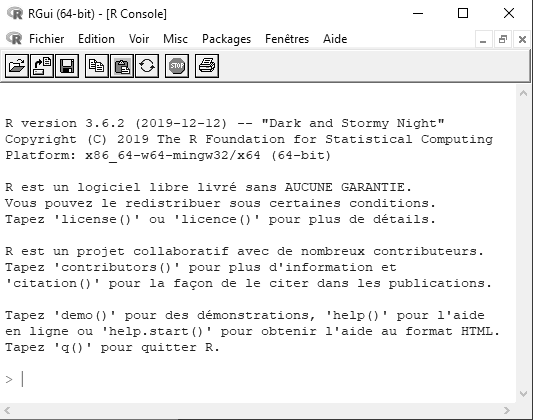
\includegraphics[width=7.53in]{myFigures/screencap_rConsoleFR} \caption{Capture d'écran de la console R sous Windows.\label{fig:screenCapConsole}}\label{fig:screenCapConsole}
\end{figure}

La console correspond à l'interface où va être interprété le code, c'est à dire à l'endroit où le code va être transformé en langage machine, exécuté par l'ordinateur, puis retransmis sous une forme lisible par des humains. Cela correspond à l'écran d'affichage d'une calculatrice (Figure \ref{fig:screenCapConsoleCal}). C'est de cette manière que R va être utilisé dans la suite de cette section.

Tout au long de ce livre, les exemples de code R apparaîtront sur fond en gris. Ils peuvent être copiés et collés directement dans la console, bien qu'il soit préférable de reproduire soit même les exemples dans la console (ou plus tard dans les scripts). Le résultat de ce qui est envoyé dans la console apparaîtra également sur fond en gris avec \texttt{\#\#} devant le code afin de bien faire la distinction entre le code et le résultat du code.

\begin{figure}
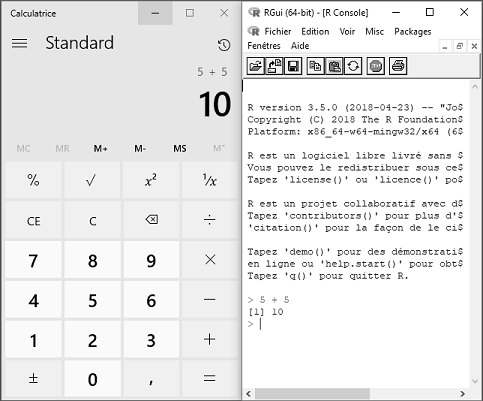
\includegraphics[width=6.71in]{myFigures/screencap_rConsoleCalculatrice} \caption{Capture d'écran de la console R sous Windows avec la calculatrice Windows.\label{fig:screenCapConsoleCal}}\label{fig:screenCapConsoleCal}
\end{figure}

\hypertarget{l011opari}{%
\subsection{Les opérateurs arithmétiques}\label{l011opari}}

\begin{Shaded}
\begin{Highlighting}[]
\DecValTok{5} \OperatorTok{+}\StringTok{ }\DecValTok{5}
\end{Highlighting}
\end{Shaded}

\begin{verbatim}
## [1] 10
\end{verbatim}

Si nous écrivons \texttt{5\ +\ 5} dans la console puis \texttt{Entrée}, le résultat apparaît précédé du chiffre {[}1{]} entre crochets. Ce chiffre correspond au numéro du résultat (dans notre cas, il n'y a qu'un seul résultat ; nous reviendrons sur cet aspect plus tard). Nous pouvons également noter dans cet exemple l'utilisation d'espaces avant et après le signe \texttt{+}. Ces espaces ne sont pas nécessaires mais permettent au code d'être plus lisible par les humains (i.e., plus agréable à lire pour nous comme pour les personnes avec qui nous serons amenés à partager notre code).
Les opérateurs aritmétiques disponibles sous R sont résumés dans la table \ref{tab:tabOpAri}.

\begin{table}[t]

\caption{\label{tab:tabOpAri}Opérateurs arithmétiques.\label{tab:tabOpAri}}
\centering
\begin{tabular}{l|l|l|l}
\hline
Label & Opérateur & Exemple & Résultat\\
\hline
Addition & + & 5 + 5 & 10\\
\hline
Soustraction & - & 5 - 5 & 0\\
\hline
Multiplication & * & 5*5 & 25\\
\hline
Division & / & 5/5 & 1\\
\hline
Puissance & \textasciicircum{} & 5\textasciicircum{}5 & 3125\\
\hline
Modulo & \%\% & 5 \%\% 5 & 0\\
\hline
Quotien Décimal & \%/\% & 5 \%/\% 5 & 1\\
\hline
\end{tabular}
\end{table}

Classiquement, les multiplications et les divisions sont prioritaires sur les additions et les soustractions. Au besoin nous pouvons utiliser des parenthèses.

\begin{Shaded}
\begin{Highlighting}[]
\DecValTok{5} \OperatorTok{+}\StringTok{ }\DecValTok{5} \OperatorTok{*}\StringTok{ }\DecValTok{2}
\end{Highlighting}
\end{Shaded}

\begin{verbatim}
## [1] 15
\end{verbatim}

\begin{Shaded}
\begin{Highlighting}[]
\NormalTok{(}\DecValTok{5} \OperatorTok{+}\StringTok{ }\DecValTok{5}\NormalTok{) }\OperatorTok{*}\StringTok{ }\DecValTok{2}
\end{Highlighting}
\end{Shaded}

\begin{verbatim}
## [1] 20
\end{verbatim}

L'opérateur modulo correspond au reste de la division euclidienne. Il est souvent utilisé en informatique par exemple pour savoir si un nombre est pair ou impair (un nombre modulo 2 va renvoyer 1 si il est impair et 0 si il est pair).

\begin{Shaded}
\begin{Highlighting}[]
\DecValTok{451} \OperatorTok\StringTok{ }\DecValTok{2}
\end{Highlighting}
\end{Shaded}

\begin{verbatim}
## [1] 1
\end{verbatim}

\begin{Shaded}
\begin{Highlighting}[]
\DecValTok{288} \OperatorTok\StringTok{ }\DecValTok{2}
\end{Highlighting}
\end{Shaded}

\begin{verbatim}
## [1] 0
\end{verbatim}

\begin{Shaded}
\begin{Highlighting}[]
\NormalTok{(}\DecValTok{5} \OperatorTok{+}\StringTok{ }\DecValTok{5} \OperatorTok{*}\StringTok{ }\DecValTok{2}\NormalTok{) }\OperatorTok\StringTok{ }\DecValTok{2}
\end{Highlighting}
\end{Shaded}

\begin{verbatim}
## [1] 1
\end{verbatim}

\begin{Shaded}
\begin{Highlighting}[]
\NormalTok{((}\DecValTok{5} \OperatorTok{+}\StringTok{ }\DecValTok{5}\NormalTok{) }\OperatorTok{*}\StringTok{ }\DecValTok{2}\NormalTok{) }\OperatorTok\StringTok{ }\DecValTok{2}
\end{Highlighting}
\end{Shaded}

\begin{verbatim}
## [1] 0
\end{verbatim}

R intègre également certaines constantes dont \texttt{pi}. Par ailleurs le signe infini est représenté par \texttt{Inf}

\begin{Shaded}
\begin{Highlighting}[]
\NormalTok{pi}
\end{Highlighting}
\end{Shaded}

\begin{verbatim}
## [1] 3.141593
\end{verbatim}

\begin{Shaded}
\begin{Highlighting}[]
\NormalTok{pi }\OperatorTok{*}\StringTok{ }\DecValTok{5}\OperatorTok{^}\DecValTok{2}
\end{Highlighting}
\end{Shaded}

\begin{verbatim}
## [1] 78.53982
\end{verbatim}

\begin{Shaded}
\begin{Highlighting}[]
\DecValTok{1}\OperatorTok{/}\DecValTok{0}
\end{Highlighting}
\end{Shaded}

\begin{verbatim}
## [1] Inf
\end{verbatim}

le \emph{style} du code est important car le code est destiné à être lisible par nous plus tard et par d'autres personnes de manière générale. Pour avoir un style lisible il est recommandé de mettre des espaces avant et après les opérateurs arithmétiques.

\hypertarget{l011opcomp}{%
\subsection{Les opérateurs de comparaison}\label{l011opcomp}}

R est cependant bien plus qu'une simple calculatrice puisque'il permet un autre type d'opérateurs : les opérateurs de comparaison. Ils servent comme leur nom l'indique à \emph{comparer} des valeurs entre elles (Table \ref{tab:tabOpCom}).

\begin{table}[t]

\caption{\label{tab:tabOpCom}Opérateurs de comparaison.\label{tab:tabOpCom}}
\centering
\begin{tabular}{l|l|l|l}
\hline
Label & Opérateur & Exemple & Résultat\\
\hline
plus petit que & < & 5 < 5 & FALSE\\
\hline
plus grand que & > & 5 > 5 & FALSE\\
\hline
plus petit ou égal à & <= & 5 <= 5 & TRUE\\
\hline
plus grand ou égal à & >= & 5 >= 5 & TRUE\\
\hline
égal à & == & 5 == 5 & TRUE\\
\hline
différent de & != & 5 != 5 & FALSE\\
\hline
\end{tabular}
\end{table}

Par exemple si nous voulons savoir si un chiffre est plus grand qu'un autre, nous pouvons écrire :

\begin{Shaded}
\begin{Highlighting}[]
\DecValTok{5} \OperatorTok{>}\StringTok{ }\DecValTok{3} 
\end{Highlighting}
\end{Shaded}

\begin{verbatim}
## [1] TRUE
\end{verbatim}

R renvoie la valeur \texttt{TRUE} si la comparasion est vraie et \texttt{FALSE} si la comparaison est fausse.

\begin{Shaded}
\begin{Highlighting}[]
\DecValTok{5} \OperatorTok{>}\StringTok{ }\DecValTok{3}
\end{Highlighting}
\end{Shaded}

\begin{verbatim}
## [1] TRUE
\end{verbatim}

\begin{Shaded}
\begin{Highlighting}[]
\DecValTok{2} \OperatorTok{<}\StringTok{ }\FloatTok{1.5}
\end{Highlighting}
\end{Shaded}

\begin{verbatim}
## [1] FALSE
\end{verbatim}

\begin{Shaded}
\begin{Highlighting}[]
\DecValTok{2} \OperatorTok{<=}\StringTok{ }\DecValTok{2}
\end{Highlighting}
\end{Shaded}

\begin{verbatim}
## [1] TRUE
\end{verbatim}

\begin{Shaded}
\begin{Highlighting}[]
\FloatTok{3.2} \OperatorTok{>=}\StringTok{ }\FloatTok{1.5}
\end{Highlighting}
\end{Shaded}

\begin{verbatim}
## [1] TRUE
\end{verbatim}

Nous pouvons combiner les opérateurs arithmétiques avec les opérateurs de comparasion.

\begin{Shaded}
\begin{Highlighting}[]
\NormalTok{(}\DecValTok{5} \OperatorTok{+}\StringTok{ }\DecValTok{8}\NormalTok{) }\OperatorTok{>}\StringTok{ }\NormalTok{(}\DecValTok{3} \OperatorTok{*}\StringTok{ }\DecValTok{45}\OperatorTok{/}\DecValTok{2}\NormalTok{) }
\end{Highlighting}
\end{Shaded}

\begin{verbatim}
## [1] FALSE
\end{verbatim}

Dans la comparasion \texttt{(5\ +\ 8)\ \textgreater{}\ (3\ *\ 45/2)} les parenthèses ne sont pas nécessaires mais elles permettent au code d'être plus facile à lire.

Un opérateur de comparaison particulier est \emph{égal à}. Nous verrons dans la section suivante que le signe \texttt{=} est réservé à un autre usage : il permet d'affecter une valeur à un objet. L'opérateur de comparaison \emph{égal à} doit donc être différent, c'est pour cela que R utilise \texttt{==}.

\begin{Shaded}
\begin{Highlighting}[]
\DecValTok{42} \OperatorTok{==}\StringTok{ }\DecValTok{53}
\end{Highlighting}
\end{Shaded}

\begin{verbatim}
## [1] FALSE
\end{verbatim}

\begin{Shaded}
\begin{Highlighting}[]
\DecValTok{58} \OperatorTok{==}\StringTok{ }\DecValTok{58}
\end{Highlighting}
\end{Shaded}

\begin{verbatim}
## [1] TRUE
\end{verbatim}

Un autre opérateur particulier est \emph{différent de}. Il est utilisé avec \emph{un point d'intérrogation} suivi de \emph{égal}, \texttt{!=}. Cet opérateur permet d'obtenir la réponse inverse à \texttt{==}.

\begin{Shaded}
\begin{Highlighting}[]
\DecValTok{42} \OperatorTok{==}\StringTok{ }\DecValTok{53}
\end{Highlighting}
\end{Shaded}

\begin{verbatim}
## [1] FALSE
\end{verbatim}

\begin{Shaded}
\begin{Highlighting}[]
\DecValTok{42} \OperatorTok{!=}\StringTok{ }\DecValTok{53}
\end{Highlighting}
\end{Shaded}

\begin{verbatim}
## [1] TRUE
\end{verbatim}

\begin{Shaded}
\begin{Highlighting}[]
\NormalTok{(}\DecValTok{3} \OperatorTok{+}\StringTok{ }\DecValTok{2}\NormalTok{) }\OperatorTok{!=}\StringTok{ }\DecValTok{5}
\end{Highlighting}
\end{Shaded}

\begin{verbatim}
## [1] FALSE
\end{verbatim}

\begin{Shaded}
\begin{Highlighting}[]
\DecValTok{10}\OperatorTok{/}\DecValTok{2} \OperatorTok{==}\StringTok{ }\DecValTok{5}
\end{Highlighting}
\end{Shaded}

\begin{verbatim}
## [1] TRUE
\end{verbatim}

R utilise \texttt{TRUE} et \texttt{FALSE} qui sont aussi des valeurs qui peuvent être testées avec les opérateurs de comparasion. Mais R attribue également une valeur à \texttt{TRUE} et \texttt{FALSE} :

\begin{Shaded}
\begin{Highlighting}[]
\OtherTok{TRUE} \OperatorTok{==}\StringTok{ }\OtherTok{TRUE}
\end{Highlighting}
\end{Shaded}

\begin{verbatim}
## [1] TRUE
\end{verbatim}

\begin{Shaded}
\begin{Highlighting}[]
\OtherTok{TRUE} \OperatorTok{>}\StringTok{ }\OtherTok{FALSE}
\end{Highlighting}
\end{Shaded}

\begin{verbatim}
## [1] TRUE
\end{verbatim}

\begin{Shaded}
\begin{Highlighting}[]
\DecValTok{1} \OperatorTok{==}\StringTok{ }\OtherTok{TRUE}
\end{Highlighting}
\end{Shaded}

\begin{verbatim}
## [1] TRUE
\end{verbatim}

\begin{Shaded}
\begin{Highlighting}[]
\DecValTok{0} \OperatorTok{==}\StringTok{ }\OtherTok{FALSE}
\end{Highlighting}
\end{Shaded}

\begin{verbatim}
## [1] TRUE
\end{verbatim}

\begin{Shaded}
\begin{Highlighting}[]
\OtherTok{TRUE} \OperatorTok{+}\StringTok{ }\DecValTok{1}
\end{Highlighting}
\end{Shaded}

\begin{verbatim}
## [1] 2
\end{verbatim}

\begin{Shaded}
\begin{Highlighting}[]
\OtherTok{FALSE} \OperatorTok{+}\StringTok{ }\DecValTok{1}
\end{Highlighting}
\end{Shaded}

\begin{verbatim}
## [1] 1
\end{verbatim}

\begin{Shaded}
\begin{Highlighting}[]
\NormalTok{(}\OtherTok{FALSE} \OperatorTok{+}\StringTok{ }\DecValTok{1}\NormalTok{) }\OperatorTok{==}\StringTok{ }\OtherTok{TRUE}
\end{Highlighting}
\end{Shaded}

\begin{verbatim}
## [1] TRUE
\end{verbatim}

La valeur de \texttt{TRUE} est de 1 et la valeur de \texttt{FALSE} est de 0. Nous verrons plus tard comment utiliser cette information dans les prochains chapitres.

R est aussi un langage relativement permissif, cela veut dire qu'il admet une certaine flexibilité dans la manière de rédiger le code. Débattre du bien fondé de cette flexibilité sort du cadre de ce livre mais nous pourrons trouver dans du code R sur Internet ou dans d'autres ouvrages le raccourcis \texttt{T} pour \texttt{TRUE} et \texttt{F} pour \texttt{FALSE}.

\begin{Shaded}
\begin{Highlighting}[]
\NormalTok{T }\OperatorTok{==}\StringTok{ }\OtherTok{TRUE}
\end{Highlighting}
\end{Shaded}

\begin{verbatim}
## [1] TRUE
\end{verbatim}

\begin{Shaded}
\begin{Highlighting}[]
\NormalTok{F }\OperatorTok{==}\StringTok{ }\OtherTok{FALSE}
\end{Highlighting}
\end{Shaded}

\begin{verbatim}
## [1] TRUE
\end{verbatim}

\begin{Shaded}
\begin{Highlighting}[]
\NormalTok{T }\OperatorTok{==}\StringTok{ }\DecValTok{1}
\end{Highlighting}
\end{Shaded}

\begin{verbatim}
## [1] TRUE
\end{verbatim}

\begin{Shaded}
\begin{Highlighting}[]
\NormalTok{F }\OperatorTok{==}\StringTok{ }\DecValTok{0}
\end{Highlighting}
\end{Shaded}

\begin{verbatim}
## [1] TRUE
\end{verbatim}

\begin{Shaded}
\begin{Highlighting}[]
\NormalTok{(F }\OperatorTok{+}\StringTok{ }\DecValTok{1}\NormalTok{) }\OperatorTok{==}\StringTok{ }\OtherTok{TRUE}
\end{Highlighting}
\end{Shaded}

\begin{verbatim}
## [1] TRUE
\end{verbatim}

Bien que cette façon de se référer à \texttt{TRUE} et \texttt{FALSE} par \texttt{T} et \texttt{F} soit assez répandue, dans ce livre nous utiliserons toujours \texttt{TRUE} et \texttt{FALSE} afin que le code soit plus facile à lire. Encore une fois l'objectif d'un code est de non seuleument être fonctionnel mais aussi d'être facile à lire et à relire.

\hypertarget{l011oplog}{%
\subsection{Les opérateurs logiques}\label{l011oplog}}

Il existe un dernier type d'opérateur, les opérateurs logiques. Ils sont utiles pour combiner des opérateurs de comparaison (Table \ref{tab:tabOpLog}).

\begin{table}[t]

\caption{\label{tab:tabOpLog}Opérateurs logiques.\label{tab:tabOpLog}}
\centering
\begin{tabular}{l|l}
\hline
Label & Operador\\
\hline
n'est pas & !\\
\hline
et & \&\\
\hline
ou & |\\
\hline
ou exclusif & xor()\\
\hline
\end{tabular}
\end{table}

\begin{Shaded}
\begin{Highlighting}[]
\OperatorTok{!}\OtherTok{TRUE}
\end{Highlighting}
\end{Shaded}

\begin{verbatim}
## [1] FALSE
\end{verbatim}

\begin{Shaded}
\begin{Highlighting}[]
\OperatorTok{!}\OtherTok{FALSE}
\end{Highlighting}
\end{Shaded}

\begin{verbatim}
## [1] TRUE
\end{verbatim}

\begin{Shaded}
\begin{Highlighting}[]
\NormalTok{((}\DecValTok{3} \OperatorTok{+}\StringTok{ }\DecValTok{2}\NormalTok{) }\OperatorTok{==}\StringTok{ }\DecValTok{5}\NormalTok{) }\OperatorTok{&}\StringTok{ }\NormalTok{((}\DecValTok{3} \OperatorTok{+}\StringTok{ }\DecValTok{3}\NormalTok{) }\OperatorTok{==}\StringTok{ }\DecValTok{5}\NormalTok{)}
\end{Highlighting}
\end{Shaded}

\begin{verbatim}
## [1] FALSE
\end{verbatim}

\begin{Shaded}
\begin{Highlighting}[]
\NormalTok{((}\DecValTok{3} \OperatorTok{+}\StringTok{ }\DecValTok{2}\NormalTok{) }\OperatorTok{==}\StringTok{ }\DecValTok{5}\NormalTok{) }\OperatorTok{&}\StringTok{ }\NormalTok{((}\DecValTok{3} \OperatorTok{+}\StringTok{ }\DecValTok{3}\NormalTok{) }\OperatorTok{==}\StringTok{ }\DecValTok{6}\NormalTok{)}
\end{Highlighting}
\end{Shaded}

\begin{verbatim}
## [1] TRUE
\end{verbatim}

\begin{Shaded}
\begin{Highlighting}[]
\NormalTok{(}\DecValTok{3} \OperatorTok{<}\StringTok{ }\DecValTok{5}\NormalTok{) }\OperatorTok{&}\StringTok{ }\NormalTok{(}\DecValTok{5} \OperatorTok{<}\StringTok{ }\DecValTok{5}\NormalTok{)}
\end{Highlighting}
\end{Shaded}

\begin{verbatim}
## [1] FALSE
\end{verbatim}

\begin{Shaded}
\begin{Highlighting}[]
\NormalTok{(}\DecValTok{3} \OperatorTok{<}\StringTok{ }\DecValTok{5}\NormalTok{) }\OperatorTok{&}\StringTok{ }\NormalTok{(}\DecValTok{5} \OperatorTok{<=}\StringTok{ }\DecValTok{5}\NormalTok{)}
\end{Highlighting}
\end{Shaded}

\begin{verbatim}
## [1] TRUE
\end{verbatim}

L'opérateur logique \texttt{xor()} correspond à un \emph{ou exclusif}. C'est à dire que l'un des deux \textbf{arguments} de la \textbf{fonction} \texttt{xor()} doit être vrai, mais pas les deux. Nous reviendrons plus tard sur les \textbf{fonctions} et leurs \textbf{arguments}, mais retenons que l'on identifie une fonction par ses parenthèses qui contiennent des arguments séparés par des virgules.

\begin{Shaded}
\begin{Highlighting}[]
\KeywordTok{xor}\NormalTok{((}\DecValTok{3} \OperatorTok{+}\StringTok{ }\DecValTok{2}\NormalTok{) }\OperatorTok{==}\StringTok{ }\DecValTok{5}\NormalTok{, (}\DecValTok{3} \OperatorTok{+}\StringTok{ }\DecValTok{3}\NormalTok{) }\OperatorTok{==}\StringTok{ }\DecValTok{6}\NormalTok{)}
\end{Highlighting}
\end{Shaded}

\begin{verbatim}
## [1] FALSE
\end{verbatim}

\begin{Shaded}
\begin{Highlighting}[]
\KeywordTok{xor}\NormalTok{((}\DecValTok{3} \OperatorTok{+}\StringTok{ }\DecValTok{2}\NormalTok{) }\OperatorTok{==}\StringTok{ }\DecValTok{5}\NormalTok{, (}\DecValTok{3} \OperatorTok{+}\StringTok{ }\DecValTok{2}\NormalTok{) }\OperatorTok{==}\StringTok{ }\DecValTok{6}\NormalTok{)}
\end{Highlighting}
\end{Shaded}

\begin{verbatim}
## [1] TRUE
\end{verbatim}

\begin{Shaded}
\begin{Highlighting}[]
\KeywordTok{xor}\NormalTok{((}\DecValTok{3} \OperatorTok{+}\StringTok{ }\DecValTok{3}\NormalTok{) }\OperatorTok{==}\StringTok{ }\DecValTok{5}\NormalTok{, (}\DecValTok{3} \OperatorTok{+}\StringTok{ }\DecValTok{2}\NormalTok{) }\OperatorTok{==}\StringTok{ }\DecValTok{6}\NormalTok{)}
\end{Highlighting}
\end{Shaded}

\begin{verbatim}
## [1] FALSE
\end{verbatim}

\begin{Shaded}
\begin{Highlighting}[]
\KeywordTok{xor}\NormalTok{((}\DecValTok{3} \OperatorTok{+}\StringTok{ }\DecValTok{3}\NormalTok{) }\OperatorTok{==}\StringTok{ }\DecValTok{5}\NormalTok{, (}\DecValTok{3} \OperatorTok{+}\StringTok{ }\DecValTok{3}\NormalTok{) }\OperatorTok{==}\StringTok{ }\DecValTok{6}\NormalTok{)}
\end{Highlighting}
\end{Shaded}

\begin{verbatim}
## [1] TRUE
\end{verbatim}

Il est recommandé que les virgules \texttt{,} soient suivies par un espace afin que le code soit plus agréable à lire.

\hypertarget{aide-sur-les-operateurs}{%
\subsection{Aide sur les opérateurs}\label{aide-sur-les-operateurs}}

Le fichier d'aide en anglais sur les opérateurs arithmétiques peut être obtenue avec la commande \texttt{?\textquotesingle{}+\textquotesingle{}} celui sur les opérateurs de comparaison avec la commande \texttt{?\textquotesingle{}==\textquotesingle{}} et celui sur les opérateurs logiques avec la commande \texttt{?\textquotesingle{}\&\textquotesingle{}}.

\hypertarget{l011object}{%
\section{La notion d'objet}\label{l011object}}

Un aspect important de la programmation avec R, mais aussi de la programmation en général est la notion d'objet. Comme indiqué sur la page web de wikipedia (\url{https://fr.wikipedia.org/wiki/Objet_(informatique)}), en informatique, un objet est un \emph{conteneur}, c'est à dire quelque chose qui va contenir de l'information. L'inforamtion contenue dans un objet peut être très diverse, mais pour le moment nous allons contenir dans un objet le chiffre 5. Pour ce faire (et pour pouvoir le réutiliser par la suite), il nous faut donner un nom à notre objet. Avec R le nom des objets ne doit pas comprendre de caractères spéciaux comme \emph{\^{}\$?\textbar+(){[}{]}\}\{}, ne doit pas commencer par un chiffre ni contenir d'espaces. Le nom de l'objet doit être représentatif de ce qu'il contient, tout en étant ni trop court ni trop long. Imaginons que notre chiffre 5 corresponde au nombre de répétitions d'une expérience. Nous voudrions lui donner un nom faisant référence à \emph{nombre} et à \emph{répétition}, que nous pourrions réduire à \emph{nbr} et \emph{rep}, respectivement. Il existe plusieurs possibilités qui sont toutes assez répandues sous R :

\begin{itemize}
\tightlist
\item
  la séparation au moyen du caractère \emph{tiret bas} : \texttt{nbr\_rep}
\item
  la séparation au moyen du caractère \emph{point} : \texttt{nbr.rep}
\item
  l'utilisation de lettres minuscules : \texttt{nbrrep}
\item
  le style \emph{lowerCamelCase} consistant en un premier mot en minuscules et des suivants avec une majuscule : \texttt{nbrRep}
\item
  le style \emph{UpperCamelCase} consistant à mettre une majuscule au début de chacun des mots : \texttt{NbrRep}
\end{itemize}

Toutes ces formes de nommer un objet sont équivalentes. Dans ce livre nous utiliserons le style \emph{lowerCamelCase}. De manière générale il faut éviter les noms trop longs comme \texttt{leNombreDeRepetitions} ou trop courts comme \texttt{nR}, et les noms ne permettant pas d'identifier le contenu comme \texttt{maVariable} ou \texttt{monChiffre}, mais aussi \texttt{a} ou \texttt{b}\ldots{}

Il existe différentes façons de définir un nom pour les objets que nous allons créer avec R. Dans ce livre nous utilisons le style \emph{lowerCamelCase}. L'important n'est pas le choix du style mais la consistence dans son choix. L'objectif est d'avoir un code fonctionnel mais également un code facile et agréable à lire.

Maintenant que nous avons choisi un nom pour notre objet, il faut le créer et faire comprendre à R que notre objet doit contenir le chiffre 5. Il existe trois façons de créer un objet sous R:

\begin{itemize}
\tightlist
\item
  avec le signe \texttt{\textless{}-}
\item
  avec le signe \texttt{=}
\item
  avec le signe \texttt{-\textgreater{}}
\end{itemize}

\begin{Shaded}
\begin{Highlighting}[]
\NormalTok{nbrRep <-}\StringTok{ }\DecValTok{5}
\NormalTok{nbrRep =}\StringTok{ }\DecValTok{5}
\DecValTok{5}\NormalTok{ ->}\StringTok{ }\NormalTok{nbrRep}
\end{Highlighting}
\end{Shaded}

Dans ce livre nous utiliserons toujours la forme \texttt{\textless{}-} par souci de consistance et aussi parce que c'est la forme la plus répandue.

\begin{Shaded}
\begin{Highlighting}[]
\NormalTok{nbrRep <-}\StringTok{ }\DecValTok{5}
\end{Highlighting}
\end{Shaded}

Nous venons de créer un objet \texttt{nbrRep} et de lui affecter la valeur 5. Cet objet est désormais disponible dans notre environnement de calcul et peut donc être utilisé. Voici quelques exemples :

\begin{Shaded}
\begin{Highlighting}[]
\NormalTok{nbrRep }\OperatorTok{+}\StringTok{ }\DecValTok{2}
\end{Highlighting}
\end{Shaded}

\begin{verbatim}
## [1] 7
\end{verbatim}

\begin{Shaded}
\begin{Highlighting}[]
\NormalTok{nbrRep }\OperatorTok{*}\StringTok{ }\DecValTok{5} \OperatorTok{-}\StringTok{ }\DecValTok{45}\OperatorTok{/}\DecValTok{56}
\end{Highlighting}
\end{Shaded}

\begin{verbatim}
## [1] 24.19643
\end{verbatim}

\begin{Shaded}
\begin{Highlighting}[]
\NormalTok{pi }\OperatorTok{*}\StringTok{ }\NormalTok{nbrRep}\OperatorTok{^}\DecValTok{2}
\end{Highlighting}
\end{Shaded}

\begin{verbatim}
## [1] 78.53982
\end{verbatim}

La valeur associée à notre objet \texttt{nbrRep} peut être modifiée de la même manière que lors de sa création :

\begin{Shaded}
\begin{Highlighting}[]
\NormalTok{nbrRep <-}\StringTok{ }\DecValTok{5}
\NormalTok{nbrRep }\OperatorTok{+}\StringTok{ }\DecValTok{2}
\end{Highlighting}
\end{Shaded}

\begin{verbatim}
## [1] 7
\end{verbatim}

\begin{Shaded}
\begin{Highlighting}[]
\NormalTok{nbrRep <-}\StringTok{ }\DecValTok{10}
\NormalTok{nbrRep }\OperatorTok{+}\StringTok{ }\DecValTok{2}
\end{Highlighting}
\end{Shaded}

\begin{verbatim}
## [1] 12
\end{verbatim}

\begin{Shaded}
\begin{Highlighting}[]
\NormalTok{nbrRep <-}\StringTok{ }\DecValTok{5} \OperatorTok{*}\StringTok{ }\DecValTok{2} \OperatorTok{+}\StringTok{ }\DecValTok{7}\OperatorTok{/}\DecValTok{3}
\NormalTok{nbrRep }\OperatorTok{+}\StringTok{ }\DecValTok{2}
\end{Highlighting}
\end{Shaded}

\begin{verbatim}
## [1] 14.33333
\end{verbatim}

L'utilisation des objets prend tout son sens lorsque nous avons des opérations complexes à réaliser et rend le code plus agréable à lire et à comprendre.

\begin{Shaded}
\begin{Highlighting}[]
\NormalTok{(}\DecValTok{5} \OperatorTok{+}\StringTok{ }\DecValTok{9}\OperatorTok{^}\DecValTok{2} \OperatorTok{-}\StringTok{ }\DecValTok{1}\OperatorTok{/}\DecValTok{18}\NormalTok{) }\OperatorTok{/}\StringTok{ }\NormalTok{(}\DecValTok{32} \OperatorTok{*}\StringTok{ }\DecValTok{45}\OperatorTok{/}\DecValTok{8} \OperatorTok{+}\StringTok{ }\DecValTok{3}\NormalTok{)}
\end{Highlighting}
\end{Shaded}

\begin{verbatim}
## [1] 0.4696418
\end{verbatim}

\begin{Shaded}
\begin{Highlighting}[]
\NormalTok{terme01 <-}\StringTok{ }\DecValTok{5} \OperatorTok{+}\StringTok{ }\DecValTok{9}\OperatorTok{^}\DecValTok{2} \OperatorTok{-}\StringTok{ }\DecValTok{1}\OperatorTok{/}\DecValTok{18}
\NormalTok{terme02 <-}\StringTok{ }\DecValTok{32} \OperatorTok{*}\StringTok{ }\DecValTok{45}\OperatorTok{/}\DecValTok{8} \OperatorTok{+}\StringTok{ }\DecValTok{3}
\NormalTok{terme01 }\OperatorTok{/}\StringTok{ }\NormalTok{terme02}
\end{Highlighting}
\end{Shaded}

\begin{verbatim}
## [1] 0.4696418
\end{verbatim}

\hypertarget{les-scripts}{%
\section{Les scripts}\label{les-scripts}}

R est un langage de programmation souvent dénommé \emph{langage de script}. Cela fait référence au fait que la plupart des utilisateurs vont écrire des petits bouts de code plutôt que des programmes entiers. R peut être utilisé comme une simple calculatrice, et dans ce cas il ne sera pas nécessaire de conserver un historique des opérations qui ont été réalisées. Mais si les opérations à réliser sont longues et complexes, il peut devenir nécessaire de pouvoir sauvegarder ce qui a été fait à un moment donné pour pouvoir poursuivre plus tard. Le fichier dans lequel seront conservées les opérations consitue ce que l'on appelle communement le script. Un script est donc un fichier contenant une succession d'informations compréhensibles par R et qu'il est possible d'exécuter.

\hypertarget{creer-un-script-et-le-documenter}{%
\subsection{Créer un script et le documenter}\label{creer-un-script-et-le-documenter}}

Pour ouvrir un nouveau script il suffit de créer un fichier texte vide qui sera édité par un éditeur de texte comme le bloc note sous Windows ou Mac OS, ou encore Gedit ou même nano sous Linux. Par convention ce fichier prend l'extension ``.r'' ou plus souvent ``.R''. C'est cette dernière convention qui sera utilisée dans ce livre. Depuis l'interface graphique de R il est possible de créer un nouveux script sous Mac OS et Windows via \emph{fichier} puis \emph{nouveau script} et \emph{enregistrer sous}.
Tout comme le nom des objets, le nom du script est important pour que nous puissions facilement identifier son contenu. Par exemple nous pourrions créer un fichier \texttt{formRConceptsBase.R} contenant les objets que nous venons de créer et les calculs effectués. Mais même avec des noms de variables et un nom de fichier bien définis, il sera difficile de se rappeler le sens de ce fichier sans une documentation accompagnant le script. Pour docummenter un script nous allons utiliser des \emph{commentaires}. Les commentaires sont des éléments qui seront identifiés par R et qui ne seront pas exécutés. Pour spécifier à R que nous allons faire un commentaire, il faut utiliser le caractère octothorpe (croisillon) \texttt{\#}. Les commentaires peuvent être insérés sur une nouvelle ligne ou en fin de ligne.

\begin{Shaded}
\begin{Highlighting}[]
\CommentTok{# creation objet nombre de repetitions}
\NormalTok{nbrRep <-}\StringTok{ }\DecValTok{5} \CommentTok{# commentaire de fin de ligne}
\end{Highlighting}
\end{Shaded}

Les commentaires peuvent aussi être utilisés pour qu'une ligne ne soit plus exécutée.

\begin{Shaded}
\begin{Highlighting}[]
\NormalTok{nbrRep <-}\StringTok{ }\DecValTok{5}
\CommentTok{# nbrRep + 5}
\end{Highlighting}
\end{Shaded}

Pour en revenir à la documentation du script, il est recommandé de commencer chacun de ses scripts par une brève description de son contenu, puis lorsque le script devient long, de le structurer en différentes parties pour faciliter sa lecture.

\begin{Shaded}
\begin{Highlighting}[]
\CommentTok{# ------------------------------------------------------------}
\CommentTok{# Voici un script pour acquérir les concepts de base }
\CommentTok{# avec R}
\CommentTok{# date de création : 25/06/2018}
\CommentTok{# auteur : François Rebaudo}
\CommentTok{# ------------------------------------------------------------}

\CommentTok{# [1] création de l'objet nombre de répétitions}
\CommentTok{# ------------------------------------------------------------}

\NormalTok{nbrRep <-}\StringTok{ }\DecValTok{5}

\CommentTok{# [2] calculs simples}
\CommentTok{# ------------------------------------------------------------}

\NormalTok{pi }\OperatorTok{*}\StringTok{ }\NormalTok{nbrRep}\OperatorTok{^}\DecValTok{2}
\end{Highlighting}
\end{Shaded}

\begin{verbatim}
## [1] 78.53982
\end{verbatim}

Pour aller plus loin sur le style de code, un guide complet de recommandations est disponible en ligne (en anglais ; \url{http://style.tidyverse.org/}).

\hypertarget{executer-un-script}{%
\subsection{Exécuter un script}\label{executer-un-script}}

Depuis que nous avons un script, nous ne travaillons plus directement dans la console. Or seule la console est capable d'interpérter le code R et de nous renvoyer les résultats que nous souhaitons obtenir. Pour l'instant la technique la plus simple consiste à copier-coller les lignes que nous souhaitons exécuter depuis notre script vers la console. A partir de maintenant nous n'allons plus utiliser les éditeurs de texte comme le bloc note mais des éditeurs spécialisés pour la confection de scripts R. C'est l'objet du chapitre suivant.

\hypertarget{conclusion}{%
\section{Conclusion}\label{conclusion}}

Félicitations, nous avons atteint la fin de ce premier chapitre sur les éléments de base de R. Nous savons:

\begin{itemize}
\tightlist
\item
  Installer R
\item
  Utiliser R comme une calculatrice
\item
  Créez des \textbf{objets} et les utiliser pour les calculs arithmétiques, les comparaisons et les tests logiques
\item
  Choisir des noms pertinents pour les objets
\item
  Créer de nouveaux \textbf{scripts}
\item
  Choisir un nom pertinent pour les fichiers de script
\item
  Exécuter le code d'un script
\item
  Documenter les scripts avec des \textbf{commentaires}
\item
  Utiliser un style de code pour le rendre agréable à lire et facile à comprendre
\end{itemize}

\hypertarget{IDE}{%
\chapter{Choisir un environnement de développement}\label{IDE}}

\hypertarget{editeurs-de-texte-et-environnement-de-developpement}{%
\section{Editeurs de texte et environnement de développement}\label{editeurs-de-texte-et-environnement-de-developpement}}

Il existe de très nombreux éditeurs de texte, le chapitre précédent a permis d'en introduire quelques uns parmi les plus simples comme le bloc note de Windows. Rapidement les limites de ces éditeurs ont rendu la tâche d'écrire un script fastidieuse. En effet, même en structurant son script avec des commentaires, il reste difficile de se répérer dans celui-ci. C'est là qu'interviennent les éditeurs de texte spécialisés qui vont permettre une écriture et une lecture agréable et simplifiée.
L'éditeur de texte pour R certainement le plus répandu est Rstudio, mais il en existe bien d'autres. Faire une liste exhaustive de toutes les solutions disponibles sort du cadre de ce livre, ainsi nous nous focaliserons sur les trois solutions que j'utilise au quotidien que sont \textbf{Notepad++}, \textbf{Rstudio}, et \textbf{Geany}.

\hypertarget{rstudio}{%
\section{RStudio}\label{rstudio}}

\begin{figure}

\includegraphics[width=7.78in]{myLogos/RStudio} \caption{Logo RStudio.\label{fig:logoRStudio}}\label{fig:logoRStudio}
\end{figure}

\hypertarget{installer-rstudio}{%
\subsection{Installer RStudio}\label{installer-rstudio}}

Le programme pour installer Rstudio se retrouve dans la partie \emph{Products} du site web de Rstudio (\url{https://www.rstudio.com/}). Nous allons installer RStudio pour un usage local (sur notre ordinateur), donc la version qui nous intéresse est \emph{Desktop}. Nous allons utiliser la version \emph{Open Source} qui est gratuite. Ensuite il nous suffit de sélectionner la version qui correspond à notre système d'exploitation, de télécharger le fichier correspondant et de l'exécuter pour lancer l'installation. Nous pouvons conserver les options par défaut tout au long de l'installation.

\hypertarget{un-script-avec-rstudio}{%
\subsection{Un script avec RStudio}\label{un-script-avec-rstudio}}

Nous pouvons alors ouvrir RStudio. Lors de la première ouverture, l'interface est divisée en deux avec à gauche la console R que nous avons vu au chapitre précédent (Figure \ref{fig:screenCapRStudio01}). Pour ouvrir un nouveau script, nous allons dans le menu \emph{File}, \emph{New File}, \emph{R script}. Par défaut ce fichier a comme nom \emph{Untitled1}. Nous avons vu au chapitre précédent l'importance de donner un nom pertinent à nos scripts, c'est pourquoi nous allons le renommer \emph{selecEnvDev.R}, dans le menu \emph{File}, avec l'option \emph{Save As\ldots{}}.
Nous avons pu noter que la partie gauche de RStudio est désormais séparée en deux, avec en bas de l'écran la console et en haut de l'écran le script.

\begin{figure}
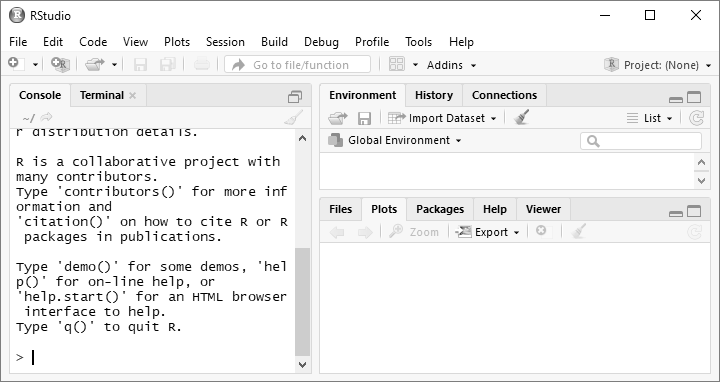
\includegraphics[width=10in]{myFigures/screencap_RStudio_01} \caption{Capture d'écran de RStudio sous Windows : fenêtre par défaut.\label{fig:screenCapRStudio01}}\label{fig:screenCapRStudio01}
\end{figure}

Nous pouvons alors commencer l'écriture de notre script avec les commentaires décrivant ce que nous allons y trouver, et y ajouter un calcul simple. Une fois que nous avons recopié le code suivant, nous pouvons sauver notre script avec la commande \texttt{CTRL\ +\ S} ou en se rendant dans \emph{File}, puis \emph{Save}.

\begin{Shaded}
\begin{Highlighting}[]
\CommentTok{# ------------------------------------------------------------}
\CommentTok{# Un script pour choisir son IDE}
\CommentTok{# créé le 27/06/2018}
\CommentTok{# modifié le 06/11/2018}
\CommentTok{# François Rebaudo}
\CommentTok{# ------------------------------------------------------------}

\CommentTok{# [1] calcul simple}
\CommentTok{# ------------------------------------------------------------}
\NormalTok{nbrRep <-}\StringTok{ }\DecValTok{5}
\NormalTok{pi }\OperatorTok{*}\StringTok{ }\NormalTok{nbrRep}\OperatorTok{^}\DecValTok{2}
\end{Highlighting}
\end{Shaded}

\begin{verbatim}
## [1] 78.53982
\end{verbatim}

Pour exécuter notre script, il suffit de sélectionner les lignes que nous souhaitons exécuter et d'utiliser la combinaison de touches \texttt{CTRL\ +\ ENTER}. Le résultat apparaît dans la console (Figure \ref{fig:screenCapRStudio02}).

\begin{figure}
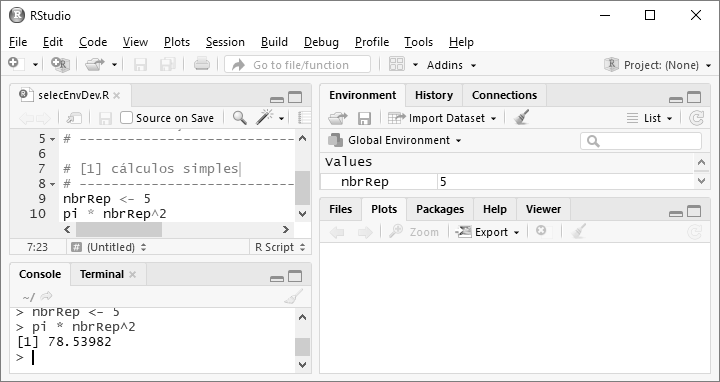
\includegraphics[width=10in]{myFigures/screencap_RStudio_02} \caption{Capture d'écran de RStudio sous Windows : exécuter un script avec CTRL + ENTER.\label{fig:screenCapRStudio02}}\label{fig:screenCapRStudio02}
\end{figure}

Nous pouvons voir que par défaut dans la partie du script les commentaires apparaissent en vert, les chiffres en bleu, et le reste du code en noir. Dans la partie de la console ce qui a été exécuté apparaît en bleu et les résultats de l'exécution en noir.
Nous pouvons également noter que dans la partie du code chaque ligne comporte un numéro correspondant au numéro de ligne à gauche sur fond gris. Il s'agit de la coloration syntaxique par défaut avec RStudio. Cette coloration syntaxique peut être modifiée en se rendant dans le menu \emph{Tools}, \emph{Global Options\ldots{}}, \emph{Appearance}, puis en choisissant un autre thème dans la liste \emph{Editor theme:}. Nous allons choisir le thème \emph{Cobalt}, puis \emph{OK} (Figure \ref{fig:screenCapRStudio03}).

\begin{figure}
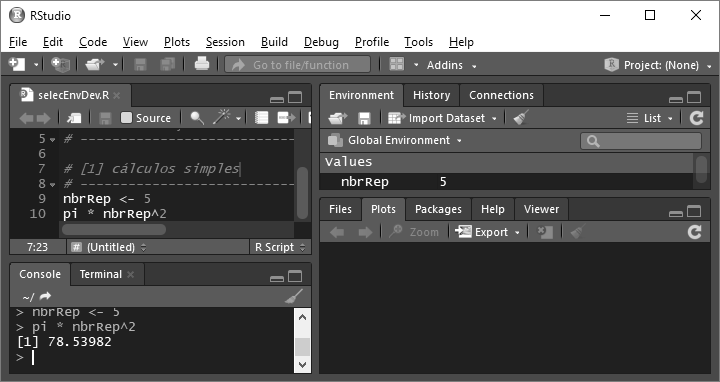
\includegraphics[width=10in]{myFigures/screencap_RStudio_03} \caption{Capture d'écran de RStudio sous Windows : changer les paramètres de coloration syntaxique.\label{fig:screenCapRStudio03}}\label{fig:screenCapRStudio03}
\end{figure}

Nous savons comment créer un nouveau script, le sauvegarder, exécuter son contenu, et changer l'apparence de RStudio. Nous verrons les nombreux autres avantages de RStudio tout au long de ce livre car c'est l'environnement de développement qui sera utilisé. Nous serons néanmois particulièrement vigilents à ce que tous les scripts développés tout au long de ce livre s'exécute de la même façon quel que soit l'environnement de développement utilisé.

\hypertarget{notepad-avec-npp2r}{%
\section{Notepad++ avec Npp2R}\label{notepad-avec-npp2r}}

\begin{figure}

\includegraphics[width=7.78in]{myLogos/Notepadpp} \caption{Logo Notepad++\label{fig:logoNotepad}}\label{fig:logoNotepad}
\end{figure}

\hypertarget{installer-notepad-pour-windows-uniquement}{%
\subsection{Installer Notepad++ (pour Windows uniquement)}\label{installer-notepad-pour-windows-uniquement}}

Le programme pour installer Notepad++ se trouve dans l'onglet \emph{Downloads} (\url{https://notepad-plus-plus.org/download/}). Vous pouvez choisir entre la version 32-bit et 64-bit (64-bit si vous ne savez pas quelle version choisir). Notepad++ seul est suffisant pour écrire un script, mais il est encore plus puissant avec \emph{Notepad to R} (\emph{Npp2R}) qui permet d'exécuter automatiquement nos script dans une console en local sur notre ordinateur ou à distance sur un serveur.

\hypertarget{installer-npp2r}{%
\subsection{Installer Npp2R}\label{installer-npp2r}}

Le programme pour installer Npp2R est hébergé sur le site de Sourceforge (\url{https://sourceforge.net/projects/npptor/}). Npp2R doit être installé après Notepad++.

\hypertarget{un-script-avec-notepad}{%
\subsection{Un script avec Notepad++}\label{un-script-avec-notepad}}

Lors de la première ouverture Notepad++ affiche un fichier vide \emph{new 1} (Figura \ref{fig:screenCapNpp01}).

\begin{figure}
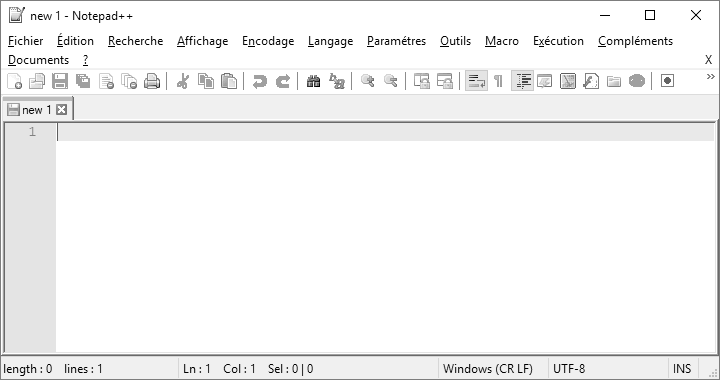
\includegraphics[width=10in]{myFigures/screencap_Npp_01} \caption{Capture d'écran de Notepad++ sous Windows : fenêtre par défaut.\label{fig:screenCapNpp01}}\label{fig:screenCapNpp01}
\end{figure}

Puisque nous avons déjà créer un script pour le tester avec RStudio, nous allons l'ouvrir à nouveau avec Notepad++. Dans \emph{Fichier}, selectionnons \emph{Ouvrir\ldots{}} puis choisir le script \emph{selecEnvDev.R} créé précédemment. Une fois le script ouvert, allons dans \emph{Langage}, puis \emph{R}, et encore une fois \emph{R}. La coloration syntaxique apparaît (Figura \ref{fig:screenCapNpp02}).

\begin{figure}
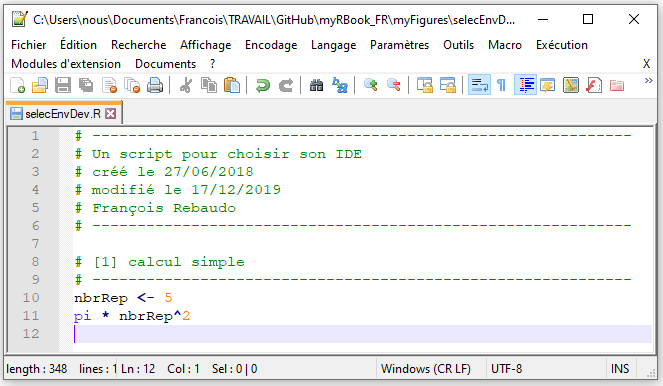
\includegraphics[width=10in]{myFigures/screencap_Npp_02} \caption{Capture d'écran de Notepad++ sous Windows : exécuter un script avec F8.\label{fig:screenCapNpp02}}\label{fig:screenCapNpp02}
\end{figure}

L'execution du script ne peut se faire que si Npp2R est en cours d'exécution. Pour se faire il est nécessaire de lancer le programme Npp2R depuis l'invite de Windows. Un icône devrait apparaître en bas de votre écran. L'exécution automatique du code depuis Notepad++ se fait en sélectionnant le code à exécuter puis en utilisant la commande \texttt{F8}. Si la commande ne fonctionne pas et que vous venez d'installer Notepad++, il est peut être nécessaire de redémarrer votre ordinateur. Si la commande fonctionne, une nouvelle fenêtre va s'ouvrir avec une consol exécutant les lignes souhaitées (Figura \ref{fig:screenCapNpp03}.

\begin{figure}
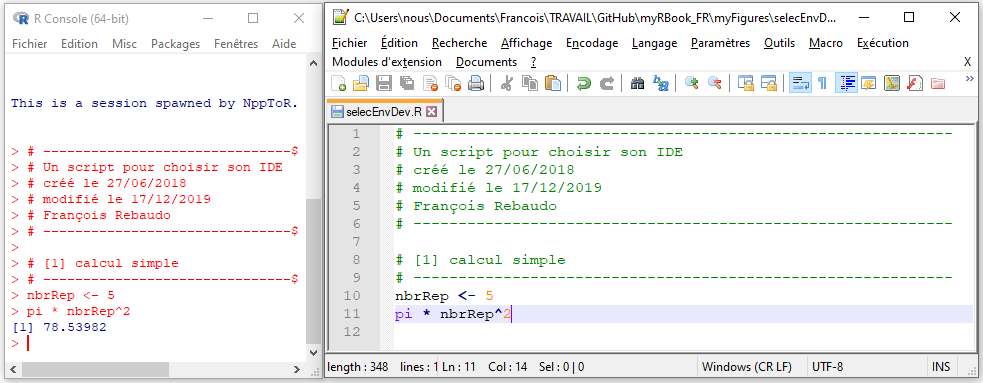
\includegraphics[width=14.83in]{myFigures/screencap_Npp_03} \caption{Capture d'écran de Notepad++ sous Windows : la console avec F8.\label{fig:screenCapNpp03}}\label{fig:screenCapNpp03}
\end{figure}

Comme pour RStudio, la coloration syntaxique peut être modifiée depuis le menu \emph{Paramètres}, et un nouveau thème peut être sélectionné (par exemple \emph{Solarized} dans la Figura \ref{fig:screenCapNpp04})

\begin{figure}
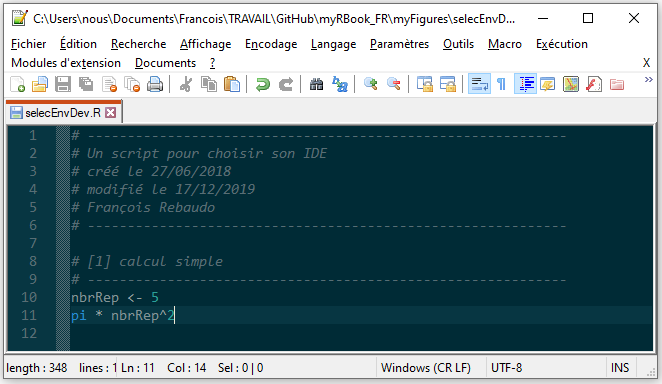
\includegraphics[width=10in]{myFigures/screencap_Npp_04} \caption{Capture d'écran de Notepad++ sous Windows : coloration syntaxique avec le thème Solarized.\label{fig:screenCapNpp04}}\label{fig:screenCapNpp04}
\end{figure}

Par rapport aux autres éditeurs de texte, Notepad++ a l'avantage d'être très léger et offre une vaste gamme d'options pour personnaliser l'écriture du code.

\hypertarget{geany-pour-linux-mac-osx-et-windows}{%
\section{Geany (pour Linux, Mac OSX et Windows)}\label{geany-pour-linux-mac-osx-et-windows}}

\begin{figure}

\includegraphics[width=7.78in]{myLogos/Geany} \caption{Logo Geany\label{fig:logoGeany}}\label{fig:logoGeany}
\end{figure}

\hypertarget{installer-geany}{%
\subsection{Installer Geany}\label{installer-geany}}

Le programme pour l'installation de Geany se trouve sous l'onglet \emph{Downloads} dans le menu de gauche \emph{Releases} de la page web (\url{https://www.geany.org/}). Ensuite il suffit de télécharger l'exécutable pour Windows ou le dmg pour Mac OSX. Les utilisateurs de Linux préfèrerons un \texttt{sudo\ apt-get\ install\ geany}.

\hypertarget{un-script-avec-geany}{%
\subsection{Un script avec Geany}\label{un-script-avec-geany}}

Lors de la première ouverture, comme pour RStudio et Notepad++, un fichier vide est créé (Figure \ref{fig:screenCapGeany01}).

\begin{figure}
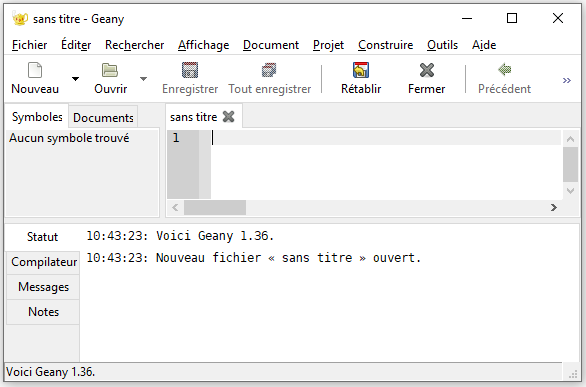
\includegraphics[width=10in]{myFigures/screencap_Geany_01} \caption{Capture d'écran de Geany sous Windows : fenêtre par défaut.\label{fig:screenCapGeany01}}\label{fig:screenCapGeany01}
\end{figure}

Nous pouvons ouvrir notre script avec \emph{Fichier}, \emph{Ouvrir} (Figure \ref{fig:screenCapGeany02}).

\begin{figure}
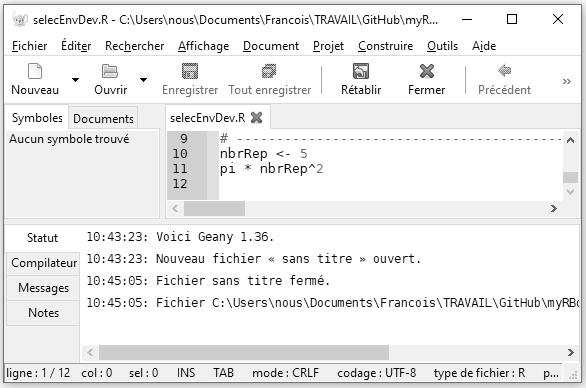
\includegraphics[width=10in]{myFigures/screencap_Geany_02} \caption{Capture d'écran de Geany sous Windows : ouvrir un script.\label{fig:screenCapGeany02}}\label{fig:screenCapGeany02}
\end{figure}

Pour exécuter notre script, la version de Geany pour Windows ne dispose pas d'un terminal intégré, ce qui rend son utilisation limitée sous ce système d'exploitation. L'exécution d'un script peut se faire en ouvrant R dans une fenêtre à part et en copiant et collant les lignes à exécuter. Sous Linux et Mac OSX, il suffit d'ouvrir R dans le terminal situé dans la partie basse de la fenêtre de Geany avec la commande \texttt{R}. Nous pouvons ensuite paramétré Geany pour qu'une combinaison de touches permette d'exécuter le code selectionné (par exemple \texttt{CTRL\ +\ R}). Pour cela il faut tout d'abord autoriser l'envoi de sélection vers le terminal (\texttt{send\_selection\_unsafe=true}) dans le fichier \texttt{geany.conf} puis choisir la commande d'envoi vers le terminal (dans \emph{Editar}, \emph{Preferencias}, \emph{Combinaciones}).
Pour changer le thème de Geany, il existe une collection de thèmes accessibles sur GitHub (\url{https://github.com/geany/geany-themes/}). Le thème peut ensuite être changé via le menu \emph{Ver}, \emph{Cambiar esquema de color\ldots{}} (un exemple avec le thème \emph{Solarized}, Figure \ref{fig:screenCapGeany03}).

\begin{figure}
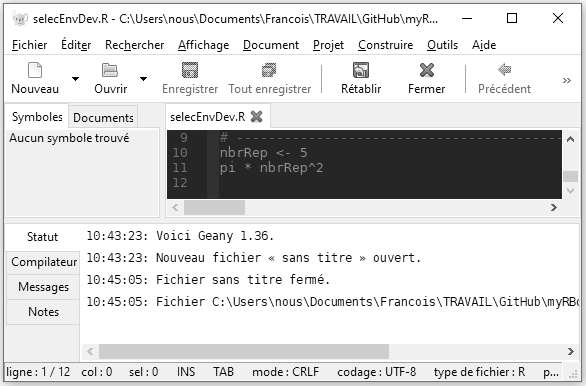
\includegraphics[width=10in]{myFigures/screencap_Geany_03} \caption{Capture d'écran de Geany sous Windows : changer les paramètres de coloration syntaxique.\label{fig:screenCapGeany03}}\label{fig:screenCapGeany03}
\end{figure}

\hypertarget{autres-solutions}{%
\section{Autres solutions}\label{autres-solutions}}

Il existe beaucoup d'autres solutions, certaines spécialisées pour R comme \textbf{Tinn-R} (\url{https://sourceforge.net/projects/tinn-r/}), et d'autres plus généralistes pour la programmation comme \textbf{Atom} (\url{https://atom.io/}), \textbf{Sublime Text} (\url{https://www.sublimetext.com/}), \textbf{Vim} (\url{https://www.vim.org/}), \textbf{Gedit} (\url{https://wiki.gnome.org/Apps/Gedit}), \textbf{GNU Emacs} (\url{https://www.gnu.org/software/emacs/}), \textbf{Jupyter} (\url{http://jupyter.org}) ou encore \textbf{Brackets} (\url{http://brackets.io/}) et \textbf{Eclipse} (\url{http://www.eclipse.org/}).

\hypertarget{conclusion-1}{%
\section{Conclusion}\label{conclusion-1}}

Felicitations, nous sommes arrivés au bout de ce chapitre sur environnements de développement pour utiliser R. Nous savons désormais :

\begin{itemize}
\tightlist
\item
  Installer RStudio, Geany ou Notepad++
\item
  Reconnaître et choisir notre environnement préféré
\end{itemize}

A partir d'ici nous allons pouvoir nous concentrer sur le language de programmation R dans un environnement facilitant le travail de lecture et d'écriture du code. C'est un grand pas en avant pour maîtriser R.

\hypertarget{dataType1}{%
\chapter{Les types de données}\label{dataType1}}

Nous avons vu précédement comment créer un objet. Un objet est comme une boîte dans laquelle nous allons \emph{stocker} de l'information. Jusqu'à présent nous n'avons stocké que des nombres mais dans ce chapitre nous allons voir qu'il est possible de stocker d'autres informations et nous allons nous attarder sur les types les plus courants. Dans ce chapitre nous allons utiliser des \textbf{fonctions} sur lesquelles nous reviendrons plus tard.

\hypertarget{le-type-numeric}{%
\section{\texorpdfstring{Le type \texttt{numeric}}{Le type numeric}}\label{le-type-numeric}}

Le type \texttt{numeric} correspond à ce que nous avons fait jusqu'à présent, stocker des nombres. Il existe deux principaux types de nombres avec R: les nombres entiers (\emph{integers}), et les nombres à virgule (\emph{double}). Par défaut R considère tous les nombres comme des nombres à virgule et attribue le type \texttt{double}.
Pour vérifier le type de données nous allons utiliser la fonction \texttt{typeof()} qui prend comme argument un objet (ou directement l'information que nous souhaitons tester). Nous pouvons également utiliser la fonction \texttt{is.double()} qui va renvoyer \texttt{TRUE} si le nombre est au format \texttt{double} et \texttt{FALSE} dans le cas contraire. La fonction générique \texttt{is.numeric()} va quant à elle renvoyer \texttt{TRUE} si l'objet est au format \texttt{numeric} et \texttt{FALSE} dans le cas contraire.

\begin{Shaded}
\begin{Highlighting}[]
\NormalTok{nbrRep <-}\StringTok{ }\DecValTok{5}
\KeywordTok{typeof}\NormalTok{(nbrRep)}
\end{Highlighting}
\end{Shaded}

\begin{verbatim}
## [1] "double"
\end{verbatim}

\begin{Shaded}
\begin{Highlighting}[]
\KeywordTok{typeof}\NormalTok{(}\FloatTok{5.32}\NormalTok{)}
\end{Highlighting}
\end{Shaded}

\begin{verbatim}
## [1] "double"
\end{verbatim}

\begin{Shaded}
\begin{Highlighting}[]
\KeywordTok{is.numeric}\NormalTok{(}\DecValTok{5}\NormalTok{)}
\end{Highlighting}
\end{Shaded}

\begin{verbatim}
## [1] TRUE
\end{verbatim}

\begin{Shaded}
\begin{Highlighting}[]
\KeywordTok{is.double}\NormalTok{(}\DecValTok{5}\NormalTok{)}
\end{Highlighting}
\end{Shaded}

\begin{verbatim}
## [1] TRUE
\end{verbatim}

Si nous voulons spécifier à R que nous allons travailler avec un nombre entier, alors il nous faut transformer notre nombre à virgule en nombre entier avec la fonction \texttt{as.integer()}. Nous pouvons également utiliser la fonction \texttt{is.integer()} qui va renvoyer \texttt{TRUE} si le nombre est au format \texttt{integer} et \texttt{FALSE} dans le cas contraire.

\begin{Shaded}
\begin{Highlighting}[]
\NormalTok{nbrRep <-}\StringTok{ }\KeywordTok{as.integer}\NormalTok{(}\DecValTok{5}\NormalTok{)}
\KeywordTok{typeof}\NormalTok{(nbrRep)}
\end{Highlighting}
\end{Shaded}

\begin{verbatim}
## [1] "integer"
\end{verbatim}

\begin{Shaded}
\begin{Highlighting}[]
\KeywordTok{typeof}\NormalTok{(}\FloatTok{5.32}\NormalTok{)}
\end{Highlighting}
\end{Shaded}

\begin{verbatim}
## [1] "double"
\end{verbatim}

\begin{Shaded}
\begin{Highlighting}[]
\KeywordTok{typeof}\NormalTok{(}\KeywordTok{as.integer}\NormalTok{(}\FloatTok{5.32}\NormalTok{))}
\end{Highlighting}
\end{Shaded}

\begin{verbatim}
## [1] "integer"
\end{verbatim}

\begin{Shaded}
\begin{Highlighting}[]
\KeywordTok{as.integer}\NormalTok{(}\FloatTok{5.32}\NormalTok{)}
\end{Highlighting}
\end{Shaded}

\begin{verbatim}
## [1] 5
\end{verbatim}

\begin{Shaded}
\begin{Highlighting}[]
\KeywordTok{as.integer}\NormalTok{(}\FloatTok{5.99}\NormalTok{)}
\end{Highlighting}
\end{Shaded}

\begin{verbatim}
## [1] 5
\end{verbatim}

\begin{Shaded}
\begin{Highlighting}[]
\KeywordTok{is.numeric}\NormalTok{(nbrRep)}
\end{Highlighting}
\end{Shaded}

\begin{verbatim}
## [1] TRUE
\end{verbatim}

Nous voyons ici que transformer un nombre comme \texttt{5.99} au format \texttt{integer} va renvoyer uniquement la partie entière, soit \texttt{5}.

\begin{Shaded}
\begin{Highlighting}[]
\KeywordTok{is.integer}\NormalTok{(}\DecValTok{5}\NormalTok{)}
\end{Highlighting}
\end{Shaded}

\begin{verbatim}
## [1] FALSE
\end{verbatim}

\begin{Shaded}
\begin{Highlighting}[]
\KeywordTok{is.numeric}\NormalTok{(}\DecValTok{5}\NormalTok{)}
\end{Highlighting}
\end{Shaded}

\begin{verbatim}
## [1] TRUE
\end{verbatim}

\begin{Shaded}
\begin{Highlighting}[]
\KeywordTok{is.integer}\NormalTok{(}\KeywordTok{as.integer}\NormalTok{(}\DecValTok{5}\NormalTok{))}
\end{Highlighting}
\end{Shaded}

\begin{verbatim}
## [1] TRUE
\end{verbatim}

\begin{Shaded}
\begin{Highlighting}[]
\KeywordTok{is.numeric}\NormalTok{(}\KeywordTok{as.integer}\NormalTok{(}\DecValTok{5}\NormalTok{))}
\end{Highlighting}
\end{Shaded}

\begin{verbatim}
## [1] TRUE
\end{verbatim}

La somme d'un nombre entier et d'un nombre à virgule renvoie un nombre à virgule.

\begin{Shaded}
\begin{Highlighting}[]
\NormalTok{sumIntDou <-}\StringTok{ }\KeywordTok{as.integer}\NormalTok{(}\DecValTok{5}\NormalTok{) }\OperatorTok{+}\StringTok{ }\FloatTok{5.2}
\KeywordTok{typeof}\NormalTok{(sumIntDou)}
\end{Highlighting}
\end{Shaded}

\begin{verbatim}
## [1] "double"
\end{verbatim}

\begin{Shaded}
\begin{Highlighting}[]
\NormalTok{sumIntInt <-}\StringTok{ }\KeywordTok{as.integer}\NormalTok{(}\DecValTok{5}\NormalTok{) }\OperatorTok{+}\StringTok{ }\KeywordTok{as.integer}\NormalTok{(}\DecValTok{5}\NormalTok{)}
\KeywordTok{typeof}\NormalTok{(sumIntInt)}
\end{Highlighting}
\end{Shaded}

\begin{verbatim}
## [1] "integer"
\end{verbatim}

Pour résumer, le type \texttt{numeric} contient deux sous-types, les types \texttt{integer} pour les nombres entiers et le type \texttt{double} pour les nombres à virgule. Par défaut R attribue le type \texttt{double} aux nombres.

Deux nombres particuliers doivent être considérés. \texttt{Inf} est un nombre de type \texttt{double}. Il désigne un nombre infini. Par exemple, \texttt{1/0} retourne \texttt{Inf} et aucun nombre ne peut être plus grand que \texttt{Inf}. \texttt{NaN} est une valeur qui signifie \texttt{Not\ a\ Number} : par exemple \texttt{0/0} retourne \texttt{NaN}. Cela peut être testé par \texttt{is.nan(0/0)}. Attention à ne pas confondre avec NA qui désigne une donnée absente (voir plus loin).

Attention, il y a un piège à l'utilisation de la fonction \texttt{is.integer()}. Elle ne nous dit pas si le nombre est un entier mais si il est du type \texttt{integer}. En effet, on peut très bien stocker un nombre entier dans une variable de type \texttt{double}.

Les nombres stockés dans une variable \texttt{integer} sont codés sur 32 bits et donc peuvent prendre des valeurs comprises entre 0 et 2\^{}32-1=4294967295. Il existe une autre façon d'indiquer à R qu'un nombre est un entier, en utilisant le suffixe L. Par exemple, \texttt{5L} est la même chose que \texttt{as.integer(5)}. L'origine de ce suffixe \texttt{L} date d'une époque où les ordinateurs utilisaient des mots de 16 bits et 32 bits étaient bien un type \texttt{Long}. Maintenant les ordinateurs utilisent des mots de 64 bits et 32 bits est plutôt court !

On ne peut pas quitter cette section sans mentionner les fonctions \protect\hyperlink{l015round}{\texttt{ceiling()}}, \protect\hyperlink{l015round}{\texttt{floor()}}, \protect\hyperlink{l015round}{\texttt{trunc()}} ou \protect\hyperlink{l015round}{\texttt{round()}} qui retournent la partie entière d'un nombre mais le laisse au type \texttt{double}. Pour en savoir plus, nous pouvons utiliser \protect\hyperlink{l015help}{l'aide de R} avec \texttt{?round}.

\begin{Shaded}
\begin{Highlighting}[]
\NormalTok{roundDou <-}\StringTok{ }\KeywordTok{round}\NormalTok{(}\FloatTok{5.2}\NormalTok{)}
\KeywordTok{typeof}\NormalTok{(roundDou)}
\end{Highlighting}
\end{Shaded}

\begin{verbatim}
## [1] "double"
\end{verbatim}

\hypertarget{le-type-character}{%
\section{\texorpdfstring{Le type \texttt{character}}{Le type character}}\label{le-type-character}}

Le type \texttt{character} correspond au texte. En effet, R permet de travailler avec du texte. pour spécifier à R que l'information contenue dans un objet est au format texte (ou de manière générale pour tous les textes), il faut utiliser les guillemets doubles (\texttt{"}), ou simples (\texttt{\textquotesingle{}}).

\begin{Shaded}
\begin{Highlighting}[]
\NormalTok{myText <-}\StringTok{ "azerty"}
\NormalTok{myText2 <-}\StringTok{ 'azerty'}
\NormalTok{myText3 <-}\StringTok{ 'azerty uiop qsdfg hjklm'}
\KeywordTok{typeof}\NormalTok{(myText3)}
\end{Highlighting}
\end{Shaded}

\begin{verbatim}
## [1] "character"
\end{verbatim}

Les guillemets doubles ou simples sont utiles si l'on souhaite mettre des guillemets dans notre texte. Nous pouvons également \emph{échapper} un caractère spécial comme un guillemet grâce au signe backslash \texttt{\textbackslash{}}.

\begin{Shaded}
\begin{Highlighting}[]
\NormalTok{myText <-}\StringTok{ "a 'ze' 'rt' y"}
\NormalTok{myText2 <-}\StringTok{ 'a "zert" y'}
\NormalTok{myText3 <-}\StringTok{ 'azerty uiop qsdfg hjklm'}
\NormalTok{myText4 <-}\StringTok{ "qwerty }\CharTok{\textbackslash{}"}\StringTok{ azerty "}
\NormalTok{myText5 <-}\StringTok{ "qwerty }\CharTok{\textbackslash{}\textbackslash{}}\StringTok{ azerty "}
\end{Highlighting}
\end{Shaded}

Par défaut lorsque nous créons un objet, son contenu n'est pas renvoyé par la console. Sur Internet ou dans de nombreux ouvrages nous pouvons retrouver le nom de l'objet sur une ligne pour renvoyer son contenu:

\begin{Shaded}
\begin{Highlighting}[]
\NormalTok{myText <-}\StringTok{ "a 'ze' 'rt' y"}
\NormalTok{myText}
\end{Highlighting}
\end{Shaded}

\begin{verbatim}
## [1] "a 'ze' 'rt' y"
\end{verbatim}

Dans ce livre nous n'utiliserons jamais cette façon de faire et préfèrerons l'utilisation de la fonction \texttt{print()}, qui permet d'afficher dans la console le contenu d'un objet. Le résultat est le même mais le code est alors plus facile à lire et plus explicite sur ce qui est fait.

\begin{Shaded}
\begin{Highlighting}[]
\NormalTok{myText <-}\StringTok{ "a 'ze' 'rt' y"}
\KeywordTok{print}\NormalTok{(myText)}
\end{Highlighting}
\end{Shaded}

\begin{verbatim}
## [1] "a 'ze' 'rt' y"
\end{verbatim}

\begin{Shaded}
\begin{Highlighting}[]
\NormalTok{nbrRep <-}\StringTok{ }\DecValTok{5}
\KeywordTok{print}\NormalTok{(nbrRep)}
\end{Highlighting}
\end{Shaded}

\begin{verbatim}
## [1] 5
\end{verbatim}

Nous pouvons également mettre des chiffres au format texte, mais il ne faut pas oublier de mettre des guillemets pour spécifier le type \texttt{character} ou utiliser la fonction \texttt{as.character()}. Une opération entre du texte et un nombre renvoie une erreur. Par exemple si l'on ajoute \texttt{10} à \texttt{"5"}, R nous signale qu'un \textbf{argument} de la \textbf{fonction} \texttt{+} n'est pas de type \texttt{numeric} et que donc l'opération n'est pas possible. Nous ne pouvons pas non plus ajouter du texte à du texte, mais verrons plus tard comment \emph{concaténer} deux \emph{chaines de texte}.

\begin{Shaded}
\begin{Highlighting}[]
\NormalTok{myText <-}\StringTok{ "qwerty"}
\KeywordTok{typeof}\NormalTok{(myText)}
\end{Highlighting}
\end{Shaded}

\begin{verbatim}
## [1] "character"
\end{verbatim}

\begin{Shaded}
\begin{Highlighting}[]
\NormalTok{myText2 <-}\StringTok{ }\DecValTok{5}
\KeywordTok{typeof}\NormalTok{(myText2)}
\end{Highlighting}
\end{Shaded}

\begin{verbatim}
## [1] "double"
\end{verbatim}

\begin{Shaded}
\begin{Highlighting}[]
\NormalTok{myText3 <-}\StringTok{ "5"}
\KeywordTok{typeof}\NormalTok{(myText3)}
\end{Highlighting}
\end{Shaded}

\begin{verbatim}
## [1] "character"
\end{verbatim}

\begin{Shaded}
\begin{Highlighting}[]
\NormalTok{myText2 }\OperatorTok{+}\StringTok{ }\DecValTok{10}
\end{Highlighting}
\end{Shaded}

\begin{verbatim}
## [1] 15
\end{verbatim}

\begin{Shaded}
\begin{Highlighting}[]
\KeywordTok{as.character}\NormalTok{(}\DecValTok{5}\NormalTok{)}
\end{Highlighting}
\end{Shaded}

\begin{verbatim}
## [1] "5"
\end{verbatim}

\begin{Shaded}
\begin{Highlighting}[]
\CommentTok{# myText3 + 10 # Error in myText3 + 10 : non-numeric argument to binary operator}
\CommentTok{# "a" + "b" # Error in "a" + "b" : non-numeric argument to binary operator}
\end{Highlighting}
\end{Shaded}

Pour résumer, le type \texttt{character} permet la saisie de texte, nous pouvons le reconnaître grâce aux guillemets simples ou doubles.

\hypertarget{le-type-factor}{%
\section{\texorpdfstring{Le type \texttt{factor}}{Le type factor}}\label{le-type-factor}}

Le type \texttt{factor} correspond aux facteurs. Les facteurs sont un choix parmi une liste finie de possibilités. Par exemple les pays sont des facteurs car il y a une liste finie de pays dans le monde à un temps donné. Un facteur peut être défini avec la fonction \texttt{factor()} ou transformé en utilisant la fonction \texttt{as.factor()}. Comme pour les autres types de donnée nous pouvons utiliser la fonction \texttt{is.factor()} pour vérifier le type de donnée. Pour avoir la liste de toutes les possibilités, il existe la fonction \texttt{levels()} (cette fonction prendra plus de sens quand nous aurons abordé les types de conteneur de l'information).

\begin{Shaded}
\begin{Highlighting}[]
\NormalTok{factor01 <-}\StringTok{ }\KeywordTok{factor}\NormalTok{(}\StringTok{"aaa"}\NormalTok{)}
\KeywordTok{print}\NormalTok{(factor01)}
\end{Highlighting}
\end{Shaded}

\begin{verbatim}
## [1] aaa
## Levels: aaa
\end{verbatim}

\begin{Shaded}
\begin{Highlighting}[]
\KeywordTok{typeof}\NormalTok{(factor01)}
\end{Highlighting}
\end{Shaded}

\begin{verbatim}
## [1] "integer"
\end{verbatim}

\begin{Shaded}
\begin{Highlighting}[]
\KeywordTok{is.factor}\NormalTok{(factor01)}
\end{Highlighting}
\end{Shaded}

\begin{verbatim}
## [1] TRUE
\end{verbatim}

\begin{Shaded}
\begin{Highlighting}[]
\KeywordTok{levels}\NormalTok{(factor01)}
\end{Highlighting}
\end{Shaded}

\begin{verbatim}
## [1] "aaa"
\end{verbatim}

Un facteur peut être transformé en texte avec la fonction \texttt{as.character()} mais également en nombre avec \texttt{as.numeric()}. Lors de la transformation en nombre chaque facteur prend la valeur de sa position dans la liste des possibilités. Dans notre cas il n'y a qu'une seule possibilité donc la fonction \texttt{as.numeric()} va renvoyer \texttt{1}:

\begin{Shaded}
\begin{Highlighting}[]
\NormalTok{factor01 <-}\StringTok{ }\KeywordTok{factor}\NormalTok{(}\StringTok{"aaa"}\NormalTok{)}
\KeywordTok{as.character}\NormalTok{(factor01)}
\end{Highlighting}
\end{Shaded}

\begin{verbatim}
## [1] "aaa"
\end{verbatim}

\begin{Shaded}
\begin{Highlighting}[]
\KeywordTok{as.numeric}\NormalTok{(factor01)}
\end{Highlighting}
\end{Shaded}

\begin{verbatim}
## [1] 1
\end{verbatim}

\hypertarget{l013logi}{%
\section{\texorpdfstring{Le type \texttt{logical}}{Le type logical}}\label{l013logi}}

Le type \texttt{logical} correspond aux valeurs \texttt{TRUE} et \texttt{FALSE} (et \texttt{NA}) que nous avons déjà vu avec les opérateurs de comparaison.

\begin{Shaded}
\begin{Highlighting}[]
\NormalTok{aLogic <-}\StringTok{ }\OtherTok{TRUE}
\KeywordTok{print}\NormalTok{(aLogic)}
\end{Highlighting}
\end{Shaded}

\begin{verbatim}
## [1] TRUE
\end{verbatim}

\begin{Shaded}
\begin{Highlighting}[]
\KeywordTok{typeof}\NormalTok{(aLogic)}
\end{Highlighting}
\end{Shaded}

\begin{verbatim}
## [1] "logical"
\end{verbatim}

\begin{Shaded}
\begin{Highlighting}[]
\KeywordTok{is.logical}\NormalTok{(aLogic)}
\end{Highlighting}
\end{Shaded}

\begin{verbatim}
## [1] TRUE
\end{verbatim}

\begin{Shaded}
\begin{Highlighting}[]
\NormalTok{aLogic }\OperatorTok{+}\StringTok{ }\DecValTok{1}
\end{Highlighting}
\end{Shaded}

\begin{verbatim}
## [1] 2
\end{verbatim}

\begin{Shaded}
\begin{Highlighting}[]
\KeywordTok{as.numeric}\NormalTok{(aLogic)}
\end{Highlighting}
\end{Shaded}

\begin{verbatim}
## [1] 1
\end{verbatim}

\begin{Shaded}
\begin{Highlighting}[]
\KeywordTok{as.character}\NormalTok{(aLogic)}
\end{Highlighting}
\end{Shaded}

\begin{verbatim}
## [1] "TRUE"
\end{verbatim}

\hypertarget{a-propos-de-na}{%
\section{\texorpdfstring{A propos de \texttt{NA}}{A propos de NA}}\label{a-propos-de-na}}

La valeur \texttt{NA} peut être utilisée pour spécifier l'absence de données ou les données manquantes. Par défaut \texttt{NA} est de type \texttt{logical} mais il peut être utilisé pour du texte, ou des nombres.

\begin{Shaded}
\begin{Highlighting}[]
\KeywordTok{print}\NormalTok{(}\OtherTok{NA}\NormalTok{)}
\end{Highlighting}
\end{Shaded}

\begin{verbatim}
## [1] NA
\end{verbatim}

\begin{Shaded}
\begin{Highlighting}[]
\KeywordTok{typeof}\NormalTok{(}\OtherTok{NA}\NormalTok{)}
\end{Highlighting}
\end{Shaded}

\begin{verbatim}
## [1] "logical"
\end{verbatim}

\begin{Shaded}
\begin{Highlighting}[]
\KeywordTok{typeof}\NormalTok{(}\KeywordTok{as.integer}\NormalTok{(}\OtherTok{NA}\NormalTok{))}
\end{Highlighting}
\end{Shaded}

\begin{verbatim}
## [1] "integer"
\end{verbatim}

\begin{Shaded}
\begin{Highlighting}[]
\KeywordTok{typeof}\NormalTok{(}\KeywordTok{as.character}\NormalTok{(}\OtherTok{NA}\NormalTok{))}
\end{Highlighting}
\end{Shaded}

\begin{verbatim}
## [1] "character"
\end{verbatim}

\begin{Shaded}
\begin{Highlighting}[]
\OtherTok{NA} \OperatorTok{==}\StringTok{ }\OtherTok{TRUE}
\end{Highlighting}
\end{Shaded}

\begin{verbatim}
## [1] NA
\end{verbatim}

\begin{Shaded}
\begin{Highlighting}[]
\OtherTok{NA} \OperatorTok{==}\StringTok{ }\OtherTok{FALSE}
\end{Highlighting}
\end{Shaded}

\begin{verbatim}
## [1] NA
\end{verbatim}

\begin{Shaded}
\begin{Highlighting}[]
\OtherTok{NA} \OperatorTok{>}\StringTok{ }\DecValTok{1}
\end{Highlighting}
\end{Shaded}

\begin{verbatim}
## [1] NA
\end{verbatim}

\begin{Shaded}
\begin{Highlighting}[]
\OtherTok{NA} \OperatorTok{+}\StringTok{ }\DecValTok{1}
\end{Highlighting}
\end{Shaded}

\begin{verbatim}
## [1] NA
\end{verbatim}

\hypertarget{conclusion-2}{%
\section{Conclusion}\label{conclusion-2}}

Felicitations, nous sommes arrivés au bout de ce chapitre sur les type de données. Nous savons désormais :

\begin{itemize}
\tightlist
\item
  Reconnaîte et faire des objets dans les principaux types de données
\item
  Transformer les types de données d'un type à un autre
\end{itemize}

Ce chapitre un peu fastidieux est la base pour aborder le prochain chapitre sur les conteneurs des données.

\hypertarget{dataType2}{%
\chapter{Les conteneurs de données}\label{dataType2}}

Jusqu'à présent nous avons fait des objets simples ne contenant qu'une seule valeur. Nous avons néanmoins pu voir qu'un objet avait différents attributs, comme sa valeur, mais aussi le type de donnée contenue. maintenant nous allons voir qu'il existe différents types de conteneurs permettant de stocker plusieurs données.

\hypertarget{l014vector}{%
\section{\texorpdfstring{Le conteneur \texttt{vector}}{Le conteneur vector}}\label{l014vector}}

Dans R, un \texttt{vector} est une combinaison de données avec la particularité que toutes les données contenues dans un \texttt{vector} sont du même type. Nous pouvons donc stocker plusieurs \texttt{numeric} ou \texttt{character} dans un \texttt{vector}, mais pas les deux. Le conteneur \texttt{vector} est important car c'est l'élément de base de R.

\hypertarget{creer-un-vector}{%
\subsection{\texorpdfstring{Créer un \texttt{vector}}{Créer un vector}}\label{creer-un-vector}}

Pour créer un \texttt{vector} nous allons utiliser la fonction \texttt{c()} qui permet de combiner des éléments en un \texttt{vector}. Les éléments à combiner doivent être séparés par des virgules.

\begin{Shaded}
\begin{Highlighting}[]
\NormalTok{miVec01 <-}\StringTok{ }\KeywordTok{c}\NormalTok{(}\DecValTok{1}\NormalTok{, }\DecValTok{2}\NormalTok{, }\DecValTok{3}\NormalTok{, }\DecValTok{4}\NormalTok{) }\CommentTok{# un vecteur de 4 éléments de type numeric ; double}
\KeywordTok{print}\NormalTok{(miVec01)}
\end{Highlighting}
\end{Shaded}

\begin{verbatim}
## [1] 1 2 3 4
\end{verbatim}

\begin{Shaded}
\begin{Highlighting}[]
\KeywordTok{typeof}\NormalTok{(miVec01)}
\end{Highlighting}
\end{Shaded}

\begin{verbatim}
## [1] "double"
\end{verbatim}

\begin{Shaded}
\begin{Highlighting}[]
\KeywordTok{is.vector}\NormalTok{(miVec01)}
\end{Highlighting}
\end{Shaded}

\begin{verbatim}
## [1] TRUE
\end{verbatim}

La fonction \texttt{is.vector()} permet de vérifier le type de conteneur.

\begin{Shaded}
\begin{Highlighting}[]
\NormalTok{miVec02 <-}\StringTok{ }\KeywordTok{c}\NormalTok{(}\StringTok{"a"}\NormalTok{, }\StringTok{"b"}\NormalTok{, }\StringTok{"c"}\NormalTok{) }
\KeywordTok{print}\NormalTok{(miVec02)}
\end{Highlighting}
\end{Shaded}

\begin{verbatim}
## [1] "a" "b" "c"
\end{verbatim}

\begin{Shaded}
\begin{Highlighting}[]
\KeywordTok{typeof}\NormalTok{(miVec02)}
\end{Highlighting}
\end{Shaded}

\begin{verbatim}
## [1] "character"
\end{verbatim}

\begin{Shaded}
\begin{Highlighting}[]
\KeywordTok{is.vector}\NormalTok{(miVec02)}
\end{Highlighting}
\end{Shaded}

\begin{verbatim}
## [1] TRUE
\end{verbatim}

\begin{Shaded}
\begin{Highlighting}[]
\NormalTok{miVec03 <-}\StringTok{ }\KeywordTok{c}\NormalTok{(}\OtherTok{TRUE}\NormalTok{, }\OtherTok{FALSE}\NormalTok{, }\OtherTok{FALSE}\NormalTok{, }\OtherTok{TRUE}\NormalTok{)}
\KeywordTok{print}\NormalTok{(miVec03)}
\end{Highlighting}
\end{Shaded}

\begin{verbatim}
## [1]  TRUE FALSE FALSE  TRUE
\end{verbatim}

\begin{Shaded}
\begin{Highlighting}[]
\KeywordTok{typeof}\NormalTok{(miVec03)}
\end{Highlighting}
\end{Shaded}

\begin{verbatim}
## [1] "logical"
\end{verbatim}

\begin{Shaded}
\begin{Highlighting}[]
\KeywordTok{is.vector}\NormalTok{(miVec03)}
\end{Highlighting}
\end{Shaded}

\begin{verbatim}
## [1] TRUE
\end{verbatim}

\begin{Shaded}
\begin{Highlighting}[]
\NormalTok{miVecNA <-}\StringTok{ }\KeywordTok{c}\NormalTok{(}\DecValTok{1}\NormalTok{, }\OtherTok{NA}\NormalTok{, }\DecValTok{3}\NormalTok{, }\OtherTok{NA}\NormalTok{, }\DecValTok{5}\NormalTok{)}
\KeywordTok{print}\NormalTok{(miVecNA)}
\end{Highlighting}
\end{Shaded}

\begin{verbatim}
## [1]  1 NA  3 NA  5
\end{verbatim}

\begin{Shaded}
\begin{Highlighting}[]
\KeywordTok{typeof}\NormalTok{(miVecNA)}
\end{Highlighting}
\end{Shaded}

\begin{verbatim}
## [1] "double"
\end{verbatim}

\begin{Shaded}
\begin{Highlighting}[]
\KeywordTok{is.vector}\NormalTok{(miVecNA)}
\end{Highlighting}
\end{Shaded}

\begin{verbatim}
## [1] TRUE
\end{verbatim}

\begin{Shaded}
\begin{Highlighting}[]
\NormalTok{miVec04 <-}\StringTok{ }\KeywordTok{c}\NormalTok{(}\DecValTok{1}\NormalTok{, }\StringTok{"a"}\NormalTok{)}
\KeywordTok{print}\NormalTok{(miVec04)}
\end{Highlighting}
\end{Shaded}

\begin{verbatim}
## [1] "1" "a"
\end{verbatim}

\begin{Shaded}
\begin{Highlighting}[]
\KeywordTok{typeof}\NormalTok{(miVec04)}
\end{Highlighting}
\end{Shaded}

\begin{verbatim}
## [1] "character"
\end{verbatim}

\begin{Shaded}
\begin{Highlighting}[]
\KeywordTok{is.vector}\NormalTok{(miVec04)}
\end{Highlighting}
\end{Shaded}

\begin{verbatim}
## [1] TRUE
\end{verbatim}

Si l'on combine différents types de données, par défaut R va chercher à transformer les éléments en un seul type. Si comme ici dans l'objet \texttt{miVec03} nous avons des \texttt{character} et des \texttt{numeric}, R va transformer tous les éléments en \texttt{character}.

\begin{Shaded}
\begin{Highlighting}[]
\NormalTok{miVec05 <-}\StringTok{ }\KeywordTok{c}\NormalTok{(}\KeywordTok{factor}\NormalTok{(}\StringTok{"abc"}\NormalTok{), }\StringTok{"def"}\NormalTok{)}
\KeywordTok{print}\NormalTok{(miVec05)}
\end{Highlighting}
\end{Shaded}

\begin{verbatim}
## [1] "1"   "def"
\end{verbatim}

\begin{Shaded}
\begin{Highlighting}[]
\KeywordTok{typeof}\NormalTok{(miVec05)}
\end{Highlighting}
\end{Shaded}

\begin{verbatim}
## [1] "character"
\end{verbatim}

\begin{Shaded}
\begin{Highlighting}[]
\NormalTok{miVec06 <-}\StringTok{ }\KeywordTok{c}\NormalTok{(}\OtherTok{TRUE}\NormalTok{, }\StringTok{"def"}\NormalTok{)}
\KeywordTok{print}\NormalTok{(miVec06)}
\end{Highlighting}
\end{Shaded}

\begin{verbatim}
## [1] "TRUE" "def"
\end{verbatim}

\begin{Shaded}
\begin{Highlighting}[]
\KeywordTok{typeof}\NormalTok{(miVec06)}
\end{Highlighting}
\end{Shaded}

\begin{verbatim}
## [1] "character"
\end{verbatim}

\begin{Shaded}
\begin{Highlighting}[]
\NormalTok{miVec07 <-}\StringTok{ }\KeywordTok{c}\NormalTok{(}\KeywordTok{factor}\NormalTok{(}\StringTok{"abc"}\NormalTok{), }\DecValTok{55}\NormalTok{)}
\KeywordTok{print}\NormalTok{(miVec07)}
\end{Highlighting}
\end{Shaded}

\begin{verbatim}
## [1]  1 55
\end{verbatim}

\begin{Shaded}
\begin{Highlighting}[]
\KeywordTok{typeof}\NormalTok{(miVec07)}
\end{Highlighting}
\end{Shaded}

\begin{verbatim}
## [1] "double"
\end{verbatim}

\begin{Shaded}
\begin{Highlighting}[]
\NormalTok{miVec08 <-}\StringTok{ }\KeywordTok{c}\NormalTok{(}\OtherTok{TRUE}\NormalTok{, }\DecValTok{55}\NormalTok{)}
\KeywordTok{print}\NormalTok{(miVec08)}
\end{Highlighting}
\end{Shaded}

\begin{verbatim}
## [1]  1 55
\end{verbatim}

\begin{Shaded}
\begin{Highlighting}[]
\KeywordTok{typeof}\NormalTok{(miVec08)}
\end{Highlighting}
\end{Shaded}

\begin{verbatim}
## [1] "double"
\end{verbatim}

Nous pouvons aussi combiner des objets existants au sein d'un \texttt{vector}.

\begin{Shaded}
\begin{Highlighting}[]
\NormalTok{miVec09 <-}\StringTok{ }\KeywordTok{c}\NormalTok{(miVec02, }\StringTok{"d"}\NormalTok{, }\StringTok{"e"}\NormalTok{, }\StringTok{"f"}\NormalTok{)}
\KeywordTok{print}\NormalTok{(miVec09)}
\end{Highlighting}
\end{Shaded}

\begin{verbatim}
## [1] "a" "b" "c" "d" "e" "f"
\end{verbatim}

\begin{Shaded}
\begin{Highlighting}[]
\NormalTok{miVec10 <-}\StringTok{ }\KeywordTok{c}\NormalTok{(}\StringTok{"aaa"}\NormalTok{, }\StringTok{"aa"}\NormalTok{, miVec09, }\StringTok{"d"}\NormalTok{, }\StringTok{"e"}\NormalTok{, }\StringTok{"f"}\NormalTok{)}
\KeywordTok{print}\NormalTok{(miVec10)}
\end{Highlighting}
\end{Shaded}

\begin{verbatim}
##  [1] "aaa" "aa"  "a"   "b"   "c"   "d"   "e"   "f"   "d"   "e"   "f"
\end{verbatim}

\begin{Shaded}
\begin{Highlighting}[]
\NormalTok{miVec11 <-}\StringTok{ }\KeywordTok{c}\NormalTok{(}\DecValTok{789}\NormalTok{, miVec01 , }\DecValTok{564}\NormalTok{)}
\KeywordTok{print}\NormalTok{(miVec11)}
\end{Highlighting}
\end{Shaded}

\begin{verbatim}
## [1] 789   1   2   3   4 564
\end{verbatim}

\hypertarget{operations-sur-un-vector}{%
\subsection{\texorpdfstring{Opérations sur un \texttt{vector}}{Opérations sur un vector}}\label{operations-sur-un-vector}}

Nous pouvons également effectuer des opération sur un \texttt{vector}.

\begin{Shaded}
\begin{Highlighting}[]
\KeywordTok{print}\NormalTok{(miVec01)}
\end{Highlighting}
\end{Shaded}

\begin{verbatim}
## [1] 1 2 3 4
\end{verbatim}

\begin{Shaded}
\begin{Highlighting}[]
\NormalTok{miVec01 }\OperatorTok{+}\StringTok{ }\DecValTok{1}
\end{Highlighting}
\end{Shaded}

\begin{verbatim}
## [1] 2 3 4 5
\end{verbatim}

\begin{Shaded}
\begin{Highlighting}[]
\NormalTok{miVec01 }\OperatorTok{-}\StringTok{ }\DecValTok{1}
\end{Highlighting}
\end{Shaded}

\begin{verbatim}
## [1] 0 1 2 3
\end{verbatim}

\begin{Shaded}
\begin{Highlighting}[]
\NormalTok{miVec01 }\OperatorTok{*}\StringTok{ }\DecValTok{2}
\end{Highlighting}
\end{Shaded}

\begin{verbatim}
## [1] 2 4 6 8
\end{verbatim}

\begin{Shaded}
\begin{Highlighting}[]
\NormalTok{miVec01 }\OperatorTok{/}\DecValTok{10}
\end{Highlighting}
\end{Shaded}

\begin{verbatim}
## [1] 0.1 0.2 0.3 0.4
\end{verbatim}

Les opérations d'un \texttt{vector} sur un autre sont aussi possibles, mais il faut veiller à ce que le nombre d'éléments d'un \texttt{vector} soit le même que l'autre, sinon R va effectuer le calcul en repartant du début. Voici un exemple pour illustrer ce que R fait:

\begin{Shaded}
\begin{Highlighting}[]
\NormalTok{miVec12 <-}\StringTok{ }\KeywordTok{c}\NormalTok{(}\DecValTok{1}\NormalTok{, }\DecValTok{1}\NormalTok{, }\DecValTok{1}\NormalTok{, }\DecValTok{1}\NormalTok{, }\DecValTok{1}\NormalTok{, }\DecValTok{1}\NormalTok{, }\DecValTok{1}\NormalTok{, }\DecValTok{1}\NormalTok{, }\DecValTok{1}\NormalTok{)}
\KeywordTok{print}\NormalTok{(miVec12)}
\end{Highlighting}
\end{Shaded}

\begin{verbatim}
## [1] 1 1 1 1 1 1 1 1 1
\end{verbatim}

\begin{Shaded}
\begin{Highlighting}[]
\NormalTok{miVec13 <-}\StringTok{ }\KeywordTok{c}\NormalTok{(}\DecValTok{10}\NormalTok{, }\DecValTok{20}\NormalTok{, }\DecValTok{30}\NormalTok{)}
\KeywordTok{print}\NormalTok{(miVec13)}
\end{Highlighting}
\end{Shaded}

\begin{verbatim}
## [1] 10 20 30
\end{verbatim}

\begin{Shaded}
\begin{Highlighting}[]
\NormalTok{miVec12 }\OperatorTok{+}\StringTok{ }\NormalTok{miVec13 }\CommentTok{# vecteurs de tailles différentes : attention au résultat}
\end{Highlighting}
\end{Shaded}

\begin{verbatim}
## [1] 11 21 31 11 21 31 11 21 31
\end{verbatim}

\begin{Shaded}
\begin{Highlighting}[]
\NormalTok{miVec14 <-}\StringTok{ }\KeywordTok{c}\NormalTok{(}\DecValTok{10}\NormalTok{, }\DecValTok{20}\NormalTok{, }\DecValTok{30}\NormalTok{, }\DecValTok{40}\NormalTok{, }\DecValTok{50}\NormalTok{, }\DecValTok{60}\NormalTok{, }\DecValTok{70}\NormalTok{, }\DecValTok{80}\NormalTok{, }\DecValTok{90}\NormalTok{)}
\KeywordTok{print}\NormalTok{(miVec14)}
\end{Highlighting}
\end{Shaded}

\begin{verbatim}
## [1] 10 20 30 40 50 60 70 80 90
\end{verbatim}

\begin{Shaded}
\begin{Highlighting}[]
\NormalTok{miVec12 }\OperatorTok{+}\StringTok{ }\NormalTok{miVec14 }\CommentTok{# les vecteurs sont de la même longueur}
\end{Highlighting}
\end{Shaded}

\begin{verbatim}
## [1] 11 21 31 41 51 61 71 81 91
\end{verbatim}

\begin{Shaded}
\begin{Highlighting}[]
\NormalTok{miVec15 <-}\StringTok{ }\KeywordTok{c}\NormalTok{(}\DecValTok{1}\NormalTok{, }\DecValTok{1}\NormalTok{, }\DecValTok{1}\NormalTok{, }\DecValTok{1}\NormalTok{)}
\KeywordTok{print}\NormalTok{(miVec15)}
\end{Highlighting}
\end{Shaded}

\begin{verbatim}
## [1] 1 1 1 1
\end{verbatim}

\begin{Shaded}
\begin{Highlighting}[]
\NormalTok{miVec15 }\OperatorTok{+}\StringTok{ }\NormalTok{miVec13 }\CommentTok{# vecteurs de tailles différentes et non multiples}
\end{Highlighting}
\end{Shaded}

\begin{verbatim}
## Warning in miVec15 + miVec13: la taille d'un objet plus long n'est pas
## multiple de la taille d'un objet plus court
\end{verbatim}

\begin{verbatim}
## [1] 11 21 31 11
\end{verbatim}

\hypertarget{acceder-aux-valeurs-dun-vector}{%
\subsection{\texorpdfstring{Accèder aux valeurs d'un \texttt{vector}}{Accèder aux valeurs d'un vector}}\label{acceder-aux-valeurs-dun-vector}}

Il souvent nécessaire de pouvoir accèder aux valeurs d'un \texttt{vector}, c'est à dire de récupérer une valeur ou un groupe de valeurs au sein d'un \texttt{vector}. Pour à un élément dans un \texttt{vector} nous utilisons les crochets \texttt{{[}{]}}. Entre les crochets, nous pouvons utiliser un numéro correspondant au numéro de l'élément dans le \texttt{vector}.

\begin{Shaded}
\begin{Highlighting}[]
\NormalTok{miVec20 <-}\StringTok{ }\KeywordTok{c}\NormalTok{(}\DecValTok{10}\NormalTok{, }\DecValTok{20}\NormalTok{, }\DecValTok{30}\NormalTok{, }\DecValTok{40}\NormalTok{, }\DecValTok{50}\NormalTok{, }\DecValTok{60}\NormalTok{, }\DecValTok{70}\NormalTok{, }\DecValTok{80}\NormalTok{, }\DecValTok{90}\NormalTok{)}
\NormalTok{miVec21 <-}\StringTok{ }\KeywordTok{c}\NormalTok{(}\StringTok{"a"}\NormalTok{, }\StringTok{"b"}\NormalTok{, }\StringTok{"c"}\NormalTok{, }\StringTok{"d"}\NormalTok{, }\StringTok{"e"}\NormalTok{, }\StringTok{"f"}\NormalTok{, }\StringTok{"g"}\NormalTok{, }\StringTok{"h"}\NormalTok{, }\StringTok{"i"}\NormalTok{)}
\KeywordTok{print}\NormalTok{(miVec20)}
\end{Highlighting}
\end{Shaded}

\begin{verbatim}
## [1] 10 20 30 40 50 60 70 80 90
\end{verbatim}

\begin{Shaded}
\begin{Highlighting}[]
\KeywordTok{print}\NormalTok{(miVec21)}
\end{Highlighting}
\end{Shaded}

\begin{verbatim}
## [1] "a" "b" "c" "d" "e" "f" "g" "h" "i"
\end{verbatim}

\begin{Shaded}
\begin{Highlighting}[]
\KeywordTok{print}\NormalTok{(miVec20[}\DecValTok{1}\NormalTok{])}
\end{Highlighting}
\end{Shaded}

\begin{verbatim}
## [1] 10
\end{verbatim}

\begin{Shaded}
\begin{Highlighting}[]
\KeywordTok{print}\NormalTok{(miVec21[}\DecValTok{3}\NormalTok{])}
\end{Highlighting}
\end{Shaded}

\begin{verbatim}
## [1] "c"
\end{verbatim}

Nous pouvons aussi utiliser la combinaison de différents éléments (un autre \texttt{vector}).

\begin{Shaded}
\begin{Highlighting}[]
\KeywordTok{print}\NormalTok{(miVec20[}\KeywordTok{c}\NormalTok{(}\DecValTok{1}\NormalTok{, }\DecValTok{5}\NormalTok{, }\DecValTok{9}\NormalTok{)])}
\end{Highlighting}
\end{Shaded}

\begin{verbatim}
## [1] 10 50 90
\end{verbatim}

\begin{Shaded}
\begin{Highlighting}[]
\KeywordTok{print}\NormalTok{(miVec21[}\KeywordTok{c}\NormalTok{(}\DecValTok{4}\NormalTok{, }\DecValTok{3}\NormalTok{, }\DecValTok{1}\NormalTok{)])}
\end{Highlighting}
\end{Shaded}

\begin{verbatim}
## [1] "d" "c" "a"
\end{verbatim}

\begin{Shaded}
\begin{Highlighting}[]
\KeywordTok{print}\NormalTok{(miVec21[}\KeywordTok{c}\NormalTok{(}\DecValTok{4}\NormalTok{, }\DecValTok{4}\NormalTok{, }\DecValTok{3}\NormalTok{, }\DecValTok{4}\NormalTok{, }\DecValTok{3}\NormalTok{, }\DecValTok{2}\NormalTok{, }\DecValTok{5}\NormalTok{)])}
\end{Highlighting}
\end{Shaded}

\begin{verbatim}
## [1] "d" "d" "c" "d" "c" "b" "e"
\end{verbatim}

Nous pouvons aussi selectionner des éléments en utilisant un opérateur de comparaison ou un opérateur logique.

\begin{Shaded}
\begin{Highlighting}[]
\KeywordTok{print}\NormalTok{(miVec20[miVec20 }\OperatorTok{>=}\StringTok{ }\DecValTok{50}\NormalTok{])}
\end{Highlighting}
\end{Shaded}

\begin{verbatim}
## [1] 50 60 70 80 90
\end{verbatim}

\begin{Shaded}
\begin{Highlighting}[]
\KeywordTok{print}\NormalTok{(miVec20[(miVec20 }\OperatorTok{>=}\StringTok{ }\DecValTok{50}\NormalTok{) }\OperatorTok{&}\StringTok{ }\NormalTok{((miVec20 }\OperatorTok{<}\StringTok{ }\DecValTok{80}\NormalTok{))])}
\end{Highlighting}
\end{Shaded}

\begin{verbatim}
## [1] 50 60 70
\end{verbatim}

\begin{Shaded}
\begin{Highlighting}[]
\KeywordTok{print}\NormalTok{(miVec20[miVec20 }\OperatorTok{!=}\StringTok{ }\DecValTok{50}\NormalTok{])}
\end{Highlighting}
\end{Shaded}

\begin{verbatim}
## [1] 10 20 30 40 60 70 80 90
\end{verbatim}

\begin{Shaded}
\begin{Highlighting}[]
\KeywordTok{print}\NormalTok{(miVec20[miVec20 }\OperatorTok{==}\StringTok{ }\DecValTok{30}\NormalTok{])}
\end{Highlighting}
\end{Shaded}

\begin{verbatim}
## [1] 30
\end{verbatim}

\begin{Shaded}
\begin{Highlighting}[]
\KeywordTok{print}\NormalTok{(miVec20[(miVec20 }\OperatorTok{==}\StringTok{ }\DecValTok{30}\NormalTok{) }\OperatorTok{|}\StringTok{ }\NormalTok{(miVec20 }\OperatorTok{==}\StringTok{ }\DecValTok{50}\NormalTok{)])}
\end{Highlighting}
\end{Shaded}

\begin{verbatim}
## [1] 30 50
\end{verbatim}

\begin{Shaded}
\begin{Highlighting}[]
\KeywordTok{print}\NormalTok{(miVec21[miVec21 }\OperatorTok{==}\StringTok{ "a"}\NormalTok{])}
\end{Highlighting}
\end{Shaded}

\begin{verbatim}
## [1] "a"
\end{verbatim}

Une autre fonctionnalité intéressante est de conditionner les éléments à sélectionner dans un \texttt{vector} en fonction d'un autre \texttt{vector}.

\begin{Shaded}
\begin{Highlighting}[]
\KeywordTok{print}\NormalTok{(miVec21[miVec20 }\OperatorTok{>=}\StringTok{ }\DecValTok{50}\NormalTok{])}
\end{Highlighting}
\end{Shaded}

\begin{verbatim}
## [1] "e" "f" "g" "h" "i"
\end{verbatim}

\begin{Shaded}
\begin{Highlighting}[]
\KeywordTok{print}\NormalTok{(miVec21[(miVec20 }\OperatorTok{>=}\StringTok{ }\DecValTok{50}\NormalTok{) }\OperatorTok{&}\StringTok{ }\NormalTok{((miVec20 }\OperatorTok{<}\StringTok{ }\DecValTok{80}\NormalTok{))])}
\end{Highlighting}
\end{Shaded}

\begin{verbatim}
## [1] "e" "f" "g"
\end{verbatim}

\begin{Shaded}
\begin{Highlighting}[]
\KeywordTok{print}\NormalTok{(miVec21[miVec20 }\OperatorTok{!=}\StringTok{ }\DecValTok{50}\NormalTok{])}
\end{Highlighting}
\end{Shaded}

\begin{verbatim}
## [1] "a" "b" "c" "d" "f" "g" "h" "i"
\end{verbatim}

\begin{Shaded}
\begin{Highlighting}[]
\KeywordTok{print}\NormalTok{(miVec21[miVec20 }\OperatorTok{==}\StringTok{ }\DecValTok{30}\NormalTok{])}
\end{Highlighting}
\end{Shaded}

\begin{verbatim}
## [1] "c"
\end{verbatim}

\begin{Shaded}
\begin{Highlighting}[]
\KeywordTok{print}\NormalTok{(miVec21[(miVec20 }\OperatorTok{==}\StringTok{ }\DecValTok{30}\NormalTok{) }\OperatorTok{|}\StringTok{ }\NormalTok{(miVec20 }\OperatorTok{==}\StringTok{ }\DecValTok{50}\NormalTok{)])}
\end{Highlighting}
\end{Shaded}

\begin{verbatim}
## [1] "c" "e"
\end{verbatim}

\begin{Shaded}
\begin{Highlighting}[]
\KeywordTok{print}\NormalTok{(miVec21[(miVec20 }\OperatorTok{==}\StringTok{ }\DecValTok{30}\NormalTok{) }\OperatorTok{|}\StringTok{ }\NormalTok{(miVec21 }\OperatorTok{==}\StringTok{ "h"}\NormalTok{)])}
\end{Highlighting}
\end{Shaded}

\begin{verbatim}
## [1] "c" "h"
\end{verbatim}

Il est aussi possible d'exclure certains éléments plutôt que de les sélectionner.

\begin{Shaded}
\begin{Highlighting}[]
\KeywordTok{print}\NormalTok{(miVec20[}\OperatorTok{-}\DecValTok{1}\NormalTok{])}
\end{Highlighting}
\end{Shaded}

\begin{verbatim}
## [1] 20 30 40 50 60 70 80 90
\end{verbatim}

\begin{Shaded}
\begin{Highlighting}[]
\KeywordTok{print}\NormalTok{(miVec21[}\OperatorTok{-}\DecValTok{5}\NormalTok{])}
\end{Highlighting}
\end{Shaded}

\begin{verbatim}
## [1] "a" "b" "c" "d" "f" "g" "h" "i"
\end{verbatim}

\begin{Shaded}
\begin{Highlighting}[]
\KeywordTok{print}\NormalTok{(miVec20[}\OperatorTok{-}\KeywordTok{c}\NormalTok{(}\DecValTok{1}\NormalTok{, }\DecValTok{2}\NormalTok{, }\DecValTok{5}\NormalTok{)])}
\end{Highlighting}
\end{Shaded}

\begin{verbatim}
## [1] 30 40 60 70 80 90
\end{verbatim}

\begin{Shaded}
\begin{Highlighting}[]
\KeywordTok{print}\NormalTok{(miVec21[}\OperatorTok{-}\KeywordTok{c}\NormalTok{(}\DecValTok{1}\NormalTok{, }\DecValTok{2}\NormalTok{, }\DecValTok{5}\NormalTok{)])}
\end{Highlighting}
\end{Shaded}

\begin{verbatim}
## [1] "c" "d" "f" "g" "h" "i"
\end{verbatim}

Les éléments d'un \texttt{vector} peuvent aussi être sélectionné sur la base d'un \texttt{vector} de type \texttt{logical}. Dans ce cas seuls les éléments avec une valeur \texttt{TRUE} seront sélectionnés.

\begin{Shaded}
\begin{Highlighting}[]
\NormalTok{miVec22 <-}\StringTok{ }\KeywordTok{c}\NormalTok{(}\OtherTok{TRUE}\NormalTok{, }\OtherTok{TRUE}\NormalTok{, }\OtherTok{FALSE}\NormalTok{, }\OtherTok{TRUE}\NormalTok{, }\OtherTok{FALSE}\NormalTok{, }\OtherTok{TRUE}\NormalTok{, }\OtherTok{FALSE}\NormalTok{, }\OtherTok{TRUE}\NormalTok{, }\OtherTok{TRUE}\NormalTok{)}
\KeywordTok{print}\NormalTok{(miVec21[miVec22])}
\end{Highlighting}
\end{Shaded}

\begin{verbatim}
## [1] "a" "b" "d" "f" "h" "i"
\end{verbatim}

\hypertarget{nommer-les-elements-dun-vector}{%
\subsection{\texorpdfstring{Nommer les éléments d'un \texttt{vector}}{Nommer les éléments d'un vector}}\label{nommer-les-elements-dun-vector}}

Les éléments d'un \texttt{vector} peuvent être nommé pour pouvoir s'y référer par la suite et opérer une sélection. La fonction \texttt{names()} permet de récupérer les noms des éléments d'un vecteur.

\begin{Shaded}
\begin{Highlighting}[]
\NormalTok{miVec23 <-}\StringTok{ }\KeywordTok{c}\NormalTok{(}\DataTypeTok{aaa =} \DecValTok{10}\NormalTok{, }\DataTypeTok{bbb =} \DecValTok{20}\NormalTok{, }\DataTypeTok{ccc =} \DecValTok{30}\NormalTok{, }\DataTypeTok{ddd =} \DecValTok{40}\NormalTok{, }\DataTypeTok{eee =} \DecValTok{50}\NormalTok{)}
\KeywordTok{print}\NormalTok{(miVec23)}
\end{Highlighting}
\end{Shaded}

\begin{verbatim}
## aaa bbb ccc ddd eee 
##  10  20  30  40  50
\end{verbatim}

\begin{Shaded}
\begin{Highlighting}[]
\KeywordTok{print}\NormalTok{(miVec23[}\StringTok{"bbb"}\NormalTok{])}
\end{Highlighting}
\end{Shaded}

\begin{verbatim}
## bbb 
##  20
\end{verbatim}

\begin{Shaded}
\begin{Highlighting}[]
\KeywordTok{print}\NormalTok{(miVec23[}\KeywordTok{c}\NormalTok{(}\StringTok{"bbb"}\NormalTok{, }\StringTok{"ccc"}\NormalTok{, }\StringTok{"bbb"}\NormalTok{)])}
\end{Highlighting}
\end{Shaded}

\begin{verbatim}
## bbb ccc bbb 
##  20  30  20
\end{verbatim}

\begin{Shaded}
\begin{Highlighting}[]
\KeywordTok{names}\NormalTok{(miVec23)}
\end{Highlighting}
\end{Shaded}

\begin{verbatim}
## [1] "aaa" "bbb" "ccc" "ddd" "eee"
\end{verbatim}

\hypertarget{modifier-les-elements-dun-vector}{%
\subsection{\texorpdfstring{Modifier les éléments d'un \texttt{vector}}{Modifier les éléments d'un vector}}\label{modifier-les-elements-dun-vector}}

Pour modifier un vecteur, nous opérons de la même façon que pour modifier un objet simple, avec le signe \texttt{\textless{}-} et l'élément ou les éléments à modifier entre crochets.

\begin{Shaded}
\begin{Highlighting}[]
\KeywordTok{print}\NormalTok{(miVec21)}
\end{Highlighting}
\end{Shaded}

\begin{verbatim}
## [1] "a" "b" "c" "d" "e" "f" "g" "h" "i"
\end{verbatim}

\begin{Shaded}
\begin{Highlighting}[]
\NormalTok{miVec21[}\DecValTok{3}\NormalTok{] <-}\StringTok{ "zzz"}
\KeywordTok{print}\NormalTok{(miVec21)}
\end{Highlighting}
\end{Shaded}

\begin{verbatim}
## [1] "a"   "b"   "zzz" "d"   "e"   "f"   "g"   "h"   "i"
\end{verbatim}

\begin{Shaded}
\begin{Highlighting}[]
\NormalTok{miVec21[(miVec20 }\OperatorTok{>=}\StringTok{ }\DecValTok{50}\NormalTok{) }\OperatorTok{&}\StringTok{ }\NormalTok{((miVec20 }\OperatorTok{<}\StringTok{ }\DecValTok{80}\NormalTok{))] <-}\StringTok{ "qwerty"}
\KeywordTok{print}\NormalTok{(miVec21)}
\end{Highlighting}
\end{Shaded}

\begin{verbatim}
## [1] "a"      "b"      "zzz"    "d"      "qwerty" "qwerty" "qwerty" "h"     
## [9] "i"
\end{verbatim}

\begin{Shaded}
\begin{Highlighting}[]
\KeywordTok{print}\NormalTok{(miVec23)}
\end{Highlighting}
\end{Shaded}

\begin{verbatim}
## aaa bbb ccc ddd eee 
##  10  20  30  40  50
\end{verbatim}

\begin{Shaded}
\begin{Highlighting}[]
\NormalTok{miVec23[}\StringTok{"ccc"}\NormalTok{] <-}\StringTok{ }\NormalTok{miVec23[}\StringTok{"ccc"}\NormalTok{] }\OperatorTok{+}\StringTok{ }\DecValTok{100}
\KeywordTok{print}\NormalTok{(miVec23)}
\end{Highlighting}
\end{Shaded}

\begin{verbatim}
## aaa bbb ccc ddd eee 
##  10  20 130  40  50
\end{verbatim}

Nous pouvons aussi changer les noms associés aux éléments d'un \texttt{vector}.

\begin{Shaded}
\begin{Highlighting}[]
\KeywordTok{print}\NormalTok{(miVec23)}
\end{Highlighting}
\end{Shaded}

\begin{verbatim}
## aaa bbb ccc ddd eee 
##  10  20 130  40  50
\end{verbatim}

\begin{Shaded}
\begin{Highlighting}[]
\KeywordTok{names}\NormalTok{(miVec23)[}\DecValTok{2}\NormalTok{] <-}\StringTok{ "bb_bb"}
\KeywordTok{print}\NormalTok{(miVec23)}
\end{Highlighting}
\end{Shaded}

\begin{verbatim}
##   aaa bb_bb   ccc   ddd   eee 
##    10    20   130    40    50
\end{verbatim}

Nous pouvons faire bien plus avec un \texttt{vector} et reviendrons sur leur manipulations et les opérations lors du chapitre sur les fonctions.

\hypertarget{l014list}{%
\section{\texorpdfstring{Le conteneur \texttt{list}}{Le conteneur list}}\label{l014list}}

Le deuxième type de conteneur que nous allons introduire est le conteneur \texttt{list}, qui est également le deuxième conteneur après le type \texttt{vector} de part son importance dans la programmation avec R. Le conteneur de type \texttt{list} permet de stocker une \textbf{liste} d'éléments. Contrairement à ce que nous avons vu précédement avec le type \texttt{vector}, les éléments du type \texttt{list} peuvent être différents (par exemple un \texttt{vector} de type \texttt{numeric}, puis un vecteur de type \texttt{character}). Les éléments du type \texttt{list} peuvent aussi être des conteneurs différents (par exemple un \texttt{vector}, puis une \texttt{list}). Le type de conteneur \texttt{list} prendra tout son sens lorsque nous aurons étudié les \textbf{boucles} et les \textbf{fonctions} de la famille \texttt{apply}.

\hypertarget{creer-une-list}{%
\subsection{\texorpdfstring{Créer une \texttt{list}}{Créer une list}}\label{creer-une-list}}

Pour créer une \texttt{list} nous allons utiliser la fonction \texttt{list()} qui prend comme argument des éléments (objets).

\begin{Shaded}
\begin{Highlighting}[]
\NormalTok{miList01 <-}\StringTok{ }\KeywordTok{list}\NormalTok{()}
\KeywordTok{print}\NormalTok{(miList01)}
\end{Highlighting}
\end{Shaded}

\begin{verbatim}
## list()
\end{verbatim}

\begin{Shaded}
\begin{Highlighting}[]
\NormalTok{miList02 <-}\StringTok{ }\KeywordTok{list}\NormalTok{(}\DecValTok{5}\NormalTok{, }\StringTok{"qwerty"}\NormalTok{, }\KeywordTok{c}\NormalTok{(}\DecValTok{4}\NormalTok{, }\DecValTok{5}\NormalTok{, }\DecValTok{6}\NormalTok{), }\KeywordTok{c}\NormalTok{(}\StringTok{"a"}\NormalTok{, }\StringTok{"b"}\NormalTok{, }\StringTok{"c"}\NormalTok{))}
\KeywordTok{print}\NormalTok{(miList02)}
\end{Highlighting}
\end{Shaded}

\begin{verbatim}
## [[1]]
## [1] 5
## 
## [[2]]
## [1] "qwerty"
## 
## [[3]]
## [1] 4 5 6
## 
## [[4]]
## [1] "a" "b" "c"
\end{verbatim}

\begin{Shaded}
\begin{Highlighting}[]
\NormalTok{miList03 <-}\StringTok{ }\KeywordTok{list}\NormalTok{(}\DecValTok{5}\NormalTok{, }\StringTok{"qwerty"}\NormalTok{, }\KeywordTok{list}\NormalTok{(}\KeywordTok{c}\NormalTok{(}\DecValTok{4}\NormalTok{, }\DecValTok{5}\NormalTok{, }\DecValTok{6}\NormalTok{), }\KeywordTok{c}\NormalTok{(}\StringTok{"a"}\NormalTok{, }\StringTok{"b"}\NormalTok{, }\StringTok{"c"}\NormalTok{)))}
\KeywordTok{print}\NormalTok{(miList03)}
\end{Highlighting}
\end{Shaded}

\begin{verbatim}
## [[1]]
## [1] 5
## 
## [[2]]
## [1] "qwerty"
## 
## [[3]]
## [[3]][[1]]
## [1] 4 5 6
## 
## [[3]][[2]]
## [1] "a" "b" "c"
\end{verbatim}

La fonction \texttt{is.list()} permet de tester si nous avons bien créer un objet de type \texttt{list}.

\begin{Shaded}
\begin{Highlighting}[]
\KeywordTok{is.list}\NormalTok{(miList02)}
\end{Highlighting}
\end{Shaded}

\begin{verbatim}
## [1] TRUE
\end{verbatim}

\begin{Shaded}
\begin{Highlighting}[]
\KeywordTok{typeof}\NormalTok{(miList02)}
\end{Highlighting}
\end{Shaded}

\begin{verbatim}
## [1] "list"
\end{verbatim}

\hypertarget{acceder-aux-valeurs-dune-list}{%
\subsection{\texorpdfstring{Accéder aux valeurs d'une \texttt{list}}{Accéder aux valeurs d'une list}}\label{acceder-aux-valeurs-dune-list}}

Les éléments du conteneur \texttt{list} sont identifiables grâce aux double crochets \texttt{{[}{[}\ {]}{]}}.

\begin{Shaded}
\begin{Highlighting}[]
\KeywordTok{print}\NormalTok{(miList02)}
\end{Highlighting}
\end{Shaded}

\begin{verbatim}
## [[1]]
## [1] 5
## 
## [[2]]
## [1] "qwerty"
## 
## [[3]]
## [1] 4 5 6
## 
## [[4]]
## [1] "a" "b" "c"
\end{verbatim}

Dans l'objet \texttt{miList02} de type \texttt{list}, il y a quatre éléments identifiables avec \texttt{{[}{[}1{]}{]}}, \texttt{{[}{[}2{]}{]}}, \texttt{{[}{[}3{]}{]}}, et \texttt{{[}{[}4{]}{]}}. Chacun des éléments est de type \texttt{vector} de taille 1 et de type \texttt{double} pour le premier élément, de taille 1 et de type \texttt{character} pour le deuxième élément, de taille 3 et de type \texttt{double} pour le troisième élément, et de taille 3 et de type \texttt{character} pour le quatrième élément.

\begin{Shaded}
\begin{Highlighting}[]
\KeywordTok{typeof}\NormalTok{(miList02)}
\end{Highlighting}
\end{Shaded}

\begin{verbatim}
## [1] "list"
\end{verbatim}

\begin{Shaded}
\begin{Highlighting}[]
\KeywordTok{print}\NormalTok{(miList02[[}\DecValTok{1}\NormalTok{]])}
\end{Highlighting}
\end{Shaded}

\begin{verbatim}
## [1] 5
\end{verbatim}

\begin{Shaded}
\begin{Highlighting}[]
\KeywordTok{typeof}\NormalTok{(miList02[[}\DecValTok{1}\NormalTok{]])}
\end{Highlighting}
\end{Shaded}

\begin{verbatim}
## [1] "double"
\end{verbatim}

\begin{Shaded}
\begin{Highlighting}[]
\KeywordTok{print}\NormalTok{(miList02[[}\DecValTok{2}\NormalTok{]])}
\end{Highlighting}
\end{Shaded}

\begin{verbatim}
## [1] "qwerty"
\end{verbatim}

\begin{Shaded}
\begin{Highlighting}[]
\KeywordTok{typeof}\NormalTok{(miList02[[}\DecValTok{2}\NormalTok{]])}
\end{Highlighting}
\end{Shaded}

\begin{verbatim}
## [1] "character"
\end{verbatim}

\begin{Shaded}
\begin{Highlighting}[]
\KeywordTok{print}\NormalTok{(miList02[[}\DecValTok{3}\NormalTok{]])}
\end{Highlighting}
\end{Shaded}

\begin{verbatim}
## [1] 4 5 6
\end{verbatim}

\begin{Shaded}
\begin{Highlighting}[]
\KeywordTok{typeof}\NormalTok{(miList02[[}\DecValTok{3}\NormalTok{]])}
\end{Highlighting}
\end{Shaded}

\begin{verbatim}
## [1] "double"
\end{verbatim}

\begin{Shaded}
\begin{Highlighting}[]
\KeywordTok{print}\NormalTok{(miList02[[}\DecValTok{4}\NormalTok{]])}
\end{Highlighting}
\end{Shaded}

\begin{verbatim}
## [1] "a" "b" "c"
\end{verbatim}

\begin{Shaded}
\begin{Highlighting}[]
\KeywordTok{typeof}\NormalTok{(miList02[[}\DecValTok{4}\NormalTok{]])}
\end{Highlighting}
\end{Shaded}

\begin{verbatim}
## [1] "character"
\end{verbatim}

L'accès au deuxième élément du \texttt{vector} situé en quatrième position de la liste se fait donc avec \texttt{miList02{[}{[}4{]}{]}{[}2{]}}. Nous utilisons un double crochet pour le quatrième élément de la \texttt{list}, puis un simple crochet pour le deuxième élément du \texttt{vector}.

\begin{Shaded}
\begin{Highlighting}[]
\KeywordTok{print}\NormalTok{(miList02[[}\DecValTok{4}\NormalTok{]][}\DecValTok{2}\NormalTok{])}
\end{Highlighting}
\end{Shaded}

\begin{verbatim}
## [1] "b"
\end{verbatim}

Comme une \texttt{list} peut contenir elle même une ou plusieurs \texttt{list}, nous pouvons accéder à l'information recherchée en combinant les doubles crochets. l'objet \texttt{miList04} est une \texttt{list} de deux éléments, les \texttt{list} \texttt{miList02} et \texttt{miList03}. L'objet \texttt{miList03} contient lui même une \texttt{list} comme élément en troisième position. Pour accéder au premier élément du \texttt{vector} en première position de l'élément en troisième position du deuxième élément de la \texttt{list} \texttt{miList04}, nous pouvons utiliser \texttt{miList04{[}{[}2{]}{]}{[}{[}3{]}{]}{[}{[}1{]}{]}{[}1{]}}. Il n'y a pas de limite quant à la profondeur des \texttt{list} mais dans la pratique il n'y que rarement besoin de faire des \texttt{list} de \texttt{list} de \texttt{list}.

\begin{Shaded}
\begin{Highlighting}[]
\NormalTok{miList04 <-}\StringTok{ }\KeywordTok{list}\NormalTok{(miList02, miList03)}
\KeywordTok{print}\NormalTok{(miList04)}
\end{Highlighting}
\end{Shaded}

\begin{verbatim}
## [[1]]
## [[1]][[1]]
## [1] 5
## 
## [[1]][[2]]
## [1] "qwerty"
## 
## [[1]][[3]]
## [1] 4 5 6
## 
## [[1]][[4]]
## [1] "a" "b" "c"
## 
## 
## [[2]]
## [[2]][[1]]
## [1] 5
## 
## [[2]][[2]]
## [1] "qwerty"
## 
## [[2]][[3]]
## [[2]][[3]][[1]]
## [1] 4 5 6
## 
## [[2]][[3]][[2]]
## [1] "a" "b" "c"
\end{verbatim}

\begin{Shaded}
\begin{Highlighting}[]
\KeywordTok{print}\NormalTok{(miList04[[}\DecValTok{2}\NormalTok{]][[}\DecValTok{3}\NormalTok{]][[}\DecValTok{1}\NormalTok{]][}\DecValTok{1}\NormalTok{])}
\end{Highlighting}
\end{Shaded}

\begin{verbatim}
## [1] 4
\end{verbatim}

Pour rendre concret l'exemple précédent, nous pouvons imaginer des espèces de foreurs de maïs (\emph{Sesamia nonagrioides} et \emph{Ostrinia nubilalis}), échantillonées dans différents sites, avec différentes abondances à quatre dates. Ici nous allons donner des noms aux éléments des listes.

\begin{Shaded}
\begin{Highlighting}[]
\NormalTok{bddInsect <-}\StringTok{ }\KeywordTok{list}\NormalTok{(}\DataTypeTok{Snonagrioides =} \KeywordTok{list}\NormalTok{(}\DataTypeTok{site01 =} \KeywordTok{c}\NormalTok{(}\DecValTok{12}\NormalTok{, }\DecValTok{5}\NormalTok{, }\DecValTok{8}\NormalTok{, }\DecValTok{7}\NormalTok{), }\DataTypeTok{site02 =} \KeywordTok{c}\NormalTok{(}\DecValTok{5}\NormalTok{, }\DecValTok{23}\NormalTok{, }\DecValTok{4}\NormalTok{, }\DecValTok{41}\NormalTok{), }\DataTypeTok{site03 =} \KeywordTok{c}\NormalTok{(}\DecValTok{12}\NormalTok{, }\DecValTok{0}\NormalTok{, }\DecValTok{0}\NormalTok{, }\DecValTok{0}\NormalTok{)), }\DataTypeTok{Onubilalis =} \KeywordTok{list}\NormalTok{(}\DataTypeTok{site01 =} \KeywordTok{c}\NormalTok{(}\DecValTok{12}\NormalTok{, }\DecValTok{1}\NormalTok{, }\DecValTok{2}\NormalTok{, }\DecValTok{3}\NormalTok{), }\DataTypeTok{site02 =} \KeywordTok{c}\NormalTok{(}\DecValTok{0}\NormalTok{, }\DecValTok{0}\NormalTok{, }\DecValTok{0}\NormalTok{, }\DecValTok{1}\NormalTok{), }\DataTypeTok{site03 =} \KeywordTok{c}\NormalTok{(}\DecValTok{1}\NormalTok{, }\DecValTok{1}\NormalTok{, }\DecValTok{2}\NormalTok{, }\DecValTok{3}\NormalTok{)))}
\KeywordTok{print}\NormalTok{(bddInsect)}
\end{Highlighting}
\end{Shaded}

\begin{verbatim}
## $Snonagrioides
## $Snonagrioides$site01
## [1] 12  5  8  7
## 
## $Snonagrioides$site02
## [1]  5 23  4 41
## 
## $Snonagrioides$site03
## [1] 12  0  0  0
## 
## 
## $Onubilalis
## $Onubilalis$site01
## [1] 12  1  2  3
## 
## $Onubilalis$site02
## [1] 0 0 0 1
## 
## $Onubilalis$site03
## [1] 1 1 2 3
\end{verbatim}

La lecture d'une ligne de code longue comme celle de la création de l'objet \texttt{bddInsect} est difficile à lire car la profondeur des éléments ne peut se déduire que grâce aux parenthèses. C'est pourquoi nous allons reorganiser le code pour lui donner plus de lisibilité grâce à l'\textbf{indentation}. L'indentation consiste à mettre l'information à des niveaux différents de telle manière que nous puissions rapidement identifier les différents niveaux d'un code. L'indentation se fait au moyen de la touche de tabulation du clavier. Nous reviendrons sur l'indentation avec plus de précisions lors du chapitre sur les \textbf{boucles}. Nous retiendrons pour le moment que si une ligne de code est trop longue, nous gagnons en lisibilité en passant à la ligne et que R va lire l'ensemble comme une seule ligne de code.

\begin{Shaded}
\begin{Highlighting}[]
\NormalTok{bddInsect <-}\StringTok{ }\KeywordTok{list}\NormalTok{(}
  \DataTypeTok{Snonagrioides =} \KeywordTok{list}\NormalTok{(}
    \DataTypeTok{site01 =} \KeywordTok{c}\NormalTok{(}\DecValTok{12}\NormalTok{, }\DecValTok{5}\NormalTok{, }\DecValTok{8}\NormalTok{, }\DecValTok{7}\NormalTok{), }
    \DataTypeTok{site02 =} \KeywordTok{c}\NormalTok{(}\DecValTok{5}\NormalTok{, }\DecValTok{23}\NormalTok{, }\DecValTok{4}\NormalTok{, }\DecValTok{41}\NormalTok{), }
    \DataTypeTok{site03 =} \KeywordTok{c}\NormalTok{(}\DecValTok{12}\NormalTok{, }\DecValTok{0}\NormalTok{, }\DecValTok{0}\NormalTok{, }\DecValTok{0}\NormalTok{)}
\NormalTok{  ), }
  \DataTypeTok{Onubilalis =} \KeywordTok{list}\NormalTok{(}
    \DataTypeTok{site01 =} \KeywordTok{c}\NormalTok{(}\DecValTok{12}\NormalTok{, }\DecValTok{1}\NormalTok{, }\DecValTok{2}\NormalTok{, }\DecValTok{3}\NormalTok{), }
    \DataTypeTok{site02 =} \KeywordTok{c}\NormalTok{(}\DecValTok{0}\NormalTok{, }\DecValTok{0}\NormalTok{, }\DecValTok{0}\NormalTok{, }\DecValTok{1}\NormalTok{), }
    \DataTypeTok{site03 =} \KeywordTok{c}\NormalTok{(}\DecValTok{1}\NormalTok{, }\DecValTok{1}\NormalTok{, }\DecValTok{2}\NormalTok{, }\DecValTok{3}\NormalTok{)}
\NormalTok{  )}
\NormalTok{)}
\end{Highlighting}
\end{Shaded}

Nous pouvons sélectionner les données d'abondance du deuxième site de la première espèce comme précédemment \texttt{bddInsect{[}{[}1{]}{]}{[}{[}2{]}{]}}, ou alternativement en utilisant les noms des éléments \texttt{bddInsect\$Snonagrioides\$site02}. Pour ce faire nous utilisons le signe \texttt{\$}, ou alors le nom des éléments avec des guillemets simples ou doubles \texttt{bddInsect{[}{[}\textquotesingle{}Snonagrioides\textquotesingle{}{]}{]}{[}{[}\textquotesingle{}site02\textquotesingle{}{]}{]}}.

\begin{Shaded}
\begin{Highlighting}[]
\KeywordTok{print}\NormalTok{(bddInsect[[}\DecValTok{1}\NormalTok{]][[}\DecValTok{2}\NormalTok{]])}
\end{Highlighting}
\end{Shaded}

\begin{verbatim}
## [1]  5 23  4 41
\end{verbatim}

\begin{Shaded}
\begin{Highlighting}[]
\KeywordTok{print}\NormalTok{(bddInsect}\OperatorTok{$}\NormalTok{Snonagrioides}\OperatorTok{$}\NormalTok{site02)}
\end{Highlighting}
\end{Shaded}

\begin{verbatim}
## [1]  5 23  4 41
\end{verbatim}

\begin{Shaded}
\begin{Highlighting}[]
\KeywordTok{print}\NormalTok{(bddInsect[[}\StringTok{'Snonagrioides'}\NormalTok{]][[}\StringTok{'site02'}\NormalTok{]])}
\end{Highlighting}
\end{Shaded}

\begin{verbatim}
## [1]  5 23  4 41
\end{verbatim}

Comme pour les vecteurs nous pouvons récupérer les noms des éléments avec la fonction \texttt{names()}.

\begin{Shaded}
\begin{Highlighting}[]
\KeywordTok{names}\NormalTok{(bddInsect)}
\end{Highlighting}
\end{Shaded}

\begin{verbatim}
## [1] "Snonagrioides" "Onubilalis"
\end{verbatim}

\begin{Shaded}
\begin{Highlighting}[]
\KeywordTok{names}\NormalTok{(bddInsect[[}\DecValTok{1}\NormalTok{]])}
\end{Highlighting}
\end{Shaded}

\begin{verbatim}
## [1] "site01" "site02" "site03"
\end{verbatim}

Lorsque nous utilisons les doubles crochets \texttt{{[}{[}{]}{]}} ou le signe \texttt{\$}, R renvoie le contenu de l'élément sélectionné. Dans notre exemple les données d'abondance sont contenues sous la forme d'un \texttt{vector}, donc R renvoie un élément de type \texttt{vector}. Si nous souhaitons sélectionner un élément d'une \texttt{list} mais en conservant le format \texttt{list}, alors nous pouvons utiliser les crochets simples \texttt{{[}{]}}.

\begin{Shaded}
\begin{Highlighting}[]
\KeywordTok{print}\NormalTok{(bddInsect[[}\DecValTok{1}\NormalTok{]][[}\DecValTok{2}\NormalTok{]])}
\end{Highlighting}
\end{Shaded}

\begin{verbatim}
## [1]  5 23  4 41
\end{verbatim}

\begin{Shaded}
\begin{Highlighting}[]
\KeywordTok{typeof}\NormalTok{(bddInsect[[}\DecValTok{1}\NormalTok{]][[}\DecValTok{2}\NormalTok{]])}
\end{Highlighting}
\end{Shaded}

\begin{verbatim}
## [1] "double"
\end{verbatim}

\begin{Shaded}
\begin{Highlighting}[]
\KeywordTok{is.list}\NormalTok{(bddInsect[[}\DecValTok{1}\NormalTok{]][[}\DecValTok{2}\NormalTok{]])}
\end{Highlighting}
\end{Shaded}

\begin{verbatim}
## [1] FALSE
\end{verbatim}

\begin{Shaded}
\begin{Highlighting}[]
\KeywordTok{print}\NormalTok{(bddInsect[[}\DecValTok{1}\NormalTok{]][}\DecValTok{2}\NormalTok{])}
\end{Highlighting}
\end{Shaded}

\begin{verbatim}
## $site02
## [1]  5 23  4 41
\end{verbatim}

\begin{Shaded}
\begin{Highlighting}[]
\KeywordTok{typeof}\NormalTok{(bddInsect[[}\DecValTok{1}\NormalTok{]][}\DecValTok{2}\NormalTok{])}
\end{Highlighting}
\end{Shaded}

\begin{verbatim}
## [1] "list"
\end{verbatim}

\begin{Shaded}
\begin{Highlighting}[]
\KeywordTok{is.list}\NormalTok{(bddInsect[[}\DecValTok{1}\NormalTok{]][}\DecValTok{2}\NormalTok{])}
\end{Highlighting}
\end{Shaded}

\begin{verbatim}
## [1] TRUE
\end{verbatim}

L'utilisation des crochets simples \texttt{{[}{]}} est utile lorsque nous souhaitons récupérer plusieurs éléments d'une \texttt{list}. Par exemple pour sélectionner les abondances d'insectes des deux premiers sites de la première espèce, nous utiliserons \texttt{bddInsect{[}{[}1{]}{]}{[}c(1,\ 2){]}} ou alternativement \texttt{bddInsect{[}{[}1{]}{]}{[}c("site01",\ "site02"){]}}.

\begin{Shaded}
\begin{Highlighting}[]
\KeywordTok{print}\NormalTok{(bddInsect[[}\DecValTok{1}\NormalTok{]][}\KeywordTok{c}\NormalTok{(}\DecValTok{1}\NormalTok{, }\DecValTok{2}\NormalTok{)])}
\end{Highlighting}
\end{Shaded}

\begin{verbatim}
## $site01
## [1] 12  5  8  7
## 
## $site02
## [1]  5 23  4 41
\end{verbatim}

\begin{Shaded}
\begin{Highlighting}[]
\KeywordTok{print}\NormalTok{(bddInsect[[}\DecValTok{1}\NormalTok{]][}\KeywordTok{c}\NormalTok{(}\StringTok{"site01"}\NormalTok{, }\StringTok{"site02"}\NormalTok{)])}
\end{Highlighting}
\end{Shaded}

\begin{verbatim}
## $site01
## [1] 12  5  8  7
## 
## $site02
## [1]  5 23  4 41
\end{verbatim}

\hypertarget{modification-dune-list}{%
\subsection{\texorpdfstring{Modification d'une \texttt{list}}{Modification d'une list}}\label{modification-dune-list}}

Une \texttt{list} peut être modifiée de la même façon que pour le conteneur \texttt{vector}, c'est à dire en se réferrant avec des crochets à l'élément que nous souhaitons modifier.

\begin{Shaded}
\begin{Highlighting}[]
\KeywordTok{print}\NormalTok{(miList02)}
\end{Highlighting}
\end{Shaded}

\begin{verbatim}
## [[1]]
## [1] 5
## 
## [[2]]
## [1] "qwerty"
## 
## [[3]]
## [1] 4 5 6
## 
## [[4]]
## [1] "a" "b" "c"
\end{verbatim}

\begin{Shaded}
\begin{Highlighting}[]
\NormalTok{miList02[[}\DecValTok{1}\NormalTok{]] <-}\StringTok{ }\DecValTok{12}
\KeywordTok{print}\NormalTok{(miList02)}
\end{Highlighting}
\end{Shaded}

\begin{verbatim}
## [[1]]
## [1] 12
## 
## [[2]]
## [1] "qwerty"
## 
## [[3]]
## [1] 4 5 6
## 
## [[4]]
## [1] "a" "b" "c"
\end{verbatim}

\begin{Shaded}
\begin{Highlighting}[]
\NormalTok{miList02[[}\DecValTok{4}\NormalTok{]] <-}\StringTok{ }\KeywordTok{c}\NormalTok{(}\StringTok{"d"}\NormalTok{, }\StringTok{"e"}\NormalTok{, }\StringTok{"f"}\NormalTok{)}
\KeywordTok{print}\NormalTok{(miList02)}
\end{Highlighting}
\end{Shaded}

\begin{verbatim}
## [[1]]
## [1] 12
## 
## [[2]]
## [1] "qwerty"
## 
## [[3]]
## [1] 4 5 6
## 
## [[4]]
## [1] "d" "e" "f"
\end{verbatim}

\begin{Shaded}
\begin{Highlighting}[]
\NormalTok{miList02[[}\DecValTok{4}\NormalTok{]] <-}\StringTok{ }\KeywordTok{c}\NormalTok{(}\StringTok{"a"}\NormalTok{, }\StringTok{"b"}\NormalTok{, }\StringTok{"c"}\NormalTok{, miList02[[}\DecValTok{4}\NormalTok{]], }\StringTok{"g"}\NormalTok{, }\StringTok{"h"}\NormalTok{, }\StringTok{"i"}\NormalTok{)}
\KeywordTok{print}\NormalTok{(miList02)}
\end{Highlighting}
\end{Shaded}

\begin{verbatim}
## [[1]]
## [1] 12
## 
## [[2]]
## [1] "qwerty"
## 
## [[3]]
## [1] 4 5 6
## 
## [[4]]
## [1] "a" "b" "c" "d" "e" "f" "g" "h" "i"
\end{verbatim}

\begin{Shaded}
\begin{Highlighting}[]
\NormalTok{miList02[[}\DecValTok{4}\NormalTok{]][}\DecValTok{5}\NormalTok{] <-}\StringTok{ "eee"}
\KeywordTok{print}\NormalTok{(miList02)}
\end{Highlighting}
\end{Shaded}

\begin{verbatim}
## [[1]]
## [1] 12
## 
## [[2]]
## [1] "qwerty"
## 
## [[3]]
## [1] 4 5 6
## 
## [[4]]
## [1] "a"   "b"   "c"   "d"   "eee" "f"   "g"   "h"   "i"
\end{verbatim}

\begin{Shaded}
\begin{Highlighting}[]
\NormalTok{miList02[[}\DecValTok{3}\NormalTok{]] <-}\StringTok{ }\NormalTok{miList02[[}\DecValTok{3}\NormalTok{]] }\OperatorTok{*}\StringTok{ }\DecValTok{10} \OperatorTok{-}\StringTok{ }\DecValTok{1}
\KeywordTok{print}\NormalTok{(miList02)}
\end{Highlighting}
\end{Shaded}

\begin{verbatim}
## [[1]]
## [1] 12
## 
## [[2]]
## [1] "qwerty"
## 
## [[3]]
## [1] 39 49 59
## 
## [[4]]
## [1] "a"   "b"   "c"   "d"   "eee" "f"   "g"   "h"   "i"
\end{verbatim}

\begin{Shaded}
\begin{Highlighting}[]
\NormalTok{miList02[[}\DecValTok{3}\NormalTok{]][}\DecValTok{2}\NormalTok{] <-}\StringTok{ }\NormalTok{miList02[[}\DecValTok{1}\NormalTok{]] }\OperatorTok{*}\StringTok{ }\DecValTok{100}
\KeywordTok{print}\NormalTok{(miList02)}
\end{Highlighting}
\end{Shaded}

\begin{verbatim}
## [[1]]
## [1] 12
## 
## [[2]]
## [1] "qwerty"
## 
## [[3]]
## [1]   39 1200   59
## 
## [[4]]
## [1] "a"   "b"   "c"   "d"   "eee" "f"   "g"   "h"   "i"
\end{verbatim}

\begin{Shaded}
\begin{Highlighting}[]
\KeywordTok{print}\NormalTok{(bddInsect)}
\end{Highlighting}
\end{Shaded}

\begin{verbatim}
## $Snonagrioides
## $Snonagrioides$site01
## [1] 12  5  8  7
## 
## $Snonagrioides$site02
## [1]  5 23  4 41
## 
## $Snonagrioides$site03
## [1] 12  0  0  0
## 
## 
## $Onubilalis
## $Onubilalis$site01
## [1] 12  1  2  3
## 
## $Onubilalis$site02
## [1] 0 0 0 1
## 
## $Onubilalis$site03
## [1] 1 1 2 3
\end{verbatim}

\begin{Shaded}
\begin{Highlighting}[]
\NormalTok{bddInsect[[}\StringTok{'Snonagrioides'}\NormalTok{]][[}\StringTok{'site02'}\NormalTok{]] <-}\StringTok{ }\KeywordTok{c}\NormalTok{(}\DecValTok{2}\NormalTok{, }\DecValTok{4}\NormalTok{, }\DecValTok{6}\NormalTok{, }\DecValTok{8}\NormalTok{)}
\KeywordTok{print}\NormalTok{(bddInsect)}
\end{Highlighting}
\end{Shaded}

\begin{verbatim}
## $Snonagrioides
## $Snonagrioides$site01
## [1] 12  5  8  7
## 
## $Snonagrioides$site02
## [1] 2 4 6 8
## 
## $Snonagrioides$site03
## [1] 12  0  0  0
## 
## 
## $Onubilalis
## $Onubilalis$site01
## [1] 12  1  2  3
## 
## $Onubilalis$site02
## [1] 0 0 0 1
## 
## $Onubilalis$site03
## [1] 1 1 2 3
\end{verbatim}

Pour combiner deux \texttt{list}, il suffit d'utiliser la fonction \texttt{c()} que nous avions utilisée pour créer un \texttt{vector}.

\begin{Shaded}
\begin{Highlighting}[]
\NormalTok{miList0203 <-}\StringTok{ }\KeywordTok{c}\NormalTok{(miList02, miList03)}
\KeywordTok{print}\NormalTok{(miList0203)}
\end{Highlighting}
\end{Shaded}

\begin{verbatim}
## [[1]]
## [1] 12
## 
## [[2]]
## [1] "qwerty"
## 
## [[3]]
## [1]   39 1200   59
## 
## [[4]]
## [1] "a"   "b"   "c"   "d"   "eee" "f"   "g"   "h"   "i"  
## 
## [[5]]
## [1] 5
## 
## [[6]]
## [1] "qwerty"
## 
## [[7]]
## [[7]][[1]]
## [1] 4 5 6
## 
## [[7]][[2]]
## [1] "a" "b" "c"
\end{verbatim}

Un objet de type \texttt{list} peut être transformé en \texttt{vector} avec la fonction \texttt{unlist()} si le format des éléments de la \texttt{list} le permet (un \texttt{vector} ne peut contenir que des élément du même type).

\begin{Shaded}
\begin{Highlighting}[]
\NormalTok{miList05 <-}\StringTok{ }\KeywordTok{list}\NormalTok{(}\StringTok{"a"}\NormalTok{, }\KeywordTok{c}\NormalTok{(}\StringTok{"b"}\NormalTok{, }\StringTok{"c"}\NormalTok{), }\StringTok{"d"}\NormalTok{)}
\KeywordTok{print}\NormalTok{(miList05)}
\end{Highlighting}
\end{Shaded}

\begin{verbatim}
## [[1]]
## [1] "a"
## 
## [[2]]
## [1] "b" "c"
## 
## [[3]]
## [1] "d"
\end{verbatim}

\begin{Shaded}
\begin{Highlighting}[]
\NormalTok{miVec24 <-}\StringTok{ }\KeywordTok{unlist}\NormalTok{(miList05)}
\KeywordTok{print}\NormalTok{(miVec24)}
\end{Highlighting}
\end{Shaded}

\begin{verbatim}
## [1] "a" "b" "c" "d"
\end{verbatim}

\begin{Shaded}
\begin{Highlighting}[]
\NormalTok{miList06 <-}\StringTok{ }\KeywordTok{list}\NormalTok{(}\KeywordTok{c}\NormalTok{(}\DecValTok{1}\NormalTok{, }\DecValTok{2}\NormalTok{, }\DecValTok{3}\NormalTok{), }\KeywordTok{c}\NormalTok{(}\DecValTok{4}\NormalTok{, }\DecValTok{5}\NormalTok{, }\DecValTok{6}\NormalTok{, }\DecValTok{7}\NormalTok{), }\DecValTok{8}\NormalTok{, }\DecValTok{9}\NormalTok{, }\KeywordTok{c}\NormalTok{(}\DecValTok{10}\NormalTok{, }\DecValTok{11}\NormalTok{))}
\KeywordTok{print}\NormalTok{(miList06)}
\end{Highlighting}
\end{Shaded}

\begin{verbatim}
## [[1]]
## [1] 1 2 3
## 
## [[2]]
## [1] 4 5 6 7
## 
## [[3]]
## [1] 8
## 
## [[4]]
## [1] 9
## 
## [[5]]
## [1] 10 11
\end{verbatim}

\begin{Shaded}
\begin{Highlighting}[]
\NormalTok{miVec25 <-}\StringTok{ }\KeywordTok{unlist}\NormalTok{(miList06)}
\KeywordTok{print}\NormalTok{(miVec25)}
\end{Highlighting}
\end{Shaded}

\begin{verbatim}
##  [1]  1  2  3  4  5  6  7  8  9 10 11
\end{verbatim}

Pour ajouter un élément à une \texttt{list}, nous pouvons utiliser la fonction \texttt{c()} ou alors les crochets doubles \texttt{{[}{[}{]}{]}}.

\begin{Shaded}
\begin{Highlighting}[]
\KeywordTok{print}\NormalTok{(miList05)}
\end{Highlighting}
\end{Shaded}

\begin{verbatim}
## [[1]]
## [1] "a"
## 
## [[2]]
## [1] "b" "c"
## 
## [[3]]
## [1] "d"
\end{verbatim}

\begin{Shaded}
\begin{Highlighting}[]
\NormalTok{miList05 <-}\StringTok{ }\KeywordTok{c}\NormalTok{(miList05, }\StringTok{"e"}\NormalTok{)}
\KeywordTok{print}\NormalTok{(miList05)}
\end{Highlighting}
\end{Shaded}

\begin{verbatim}
## [[1]]
## [1] "a"
## 
## [[2]]
## [1] "b" "c"
## 
## [[3]]
## [1] "d"
## 
## [[4]]
## [1] "e"
\end{verbatim}

\begin{Shaded}
\begin{Highlighting}[]
\NormalTok{miList05[[}\DecValTok{5}\NormalTok{]] <-}\StringTok{ }\KeywordTok{c}\NormalTok{(}\StringTok{"fgh"}\NormalTok{, }\StringTok{"ijk"}\NormalTok{)}
\KeywordTok{print}\NormalTok{(miList05)}
\end{Highlighting}
\end{Shaded}

\begin{verbatim}
## [[1]]
## [1] "a"
## 
## [[2]]
## [1] "b" "c"
## 
## [[3]]
## [1] "d"
## 
## [[4]]
## [1] "e"
## 
## [[5]]
## [1] "fgh" "ijk"
\end{verbatim}

Pour supprimer un élément à une \texttt{list}, la technique la plus rapide consiste à attribuer la valeur \texttt{NULL} à l'élément à supprimer.

\begin{Shaded}
\begin{Highlighting}[]
\KeywordTok{print}\NormalTok{(miList05)}
\end{Highlighting}
\end{Shaded}

\begin{verbatim}
## [[1]]
## [1] "a"
## 
## [[2]]
## [1] "b" "c"
## 
## [[3]]
## [1] "d"
## 
## [[4]]
## [1] "e"
## 
## [[5]]
## [1] "fgh" "ijk"
\end{verbatim}

\begin{Shaded}
\begin{Highlighting}[]
\NormalTok{miList05[[}\DecValTok{2}\NormalTok{]] <-}\StringTok{ }\OtherTok{NULL}
\KeywordTok{print}\NormalTok{(miList05)}
\end{Highlighting}
\end{Shaded}

\begin{verbatim}
## [[1]]
## [1] "a"
## 
## [[2]]
## [1] "d"
## 
## [[3]]
## [1] "e"
## 
## [[4]]
## [1] "fgh" "ijk"
\end{verbatim}

\hypertarget{l014dataframe}{%
\section{\texorpdfstring{Le conteneur \texttt{data.frame}}{Le conteneur data.frame}}\label{l014dataframe}}

Le conteneur \texttt{data.frame} peut être assimilé à un \emph{tableau}. Il s'agit en fait d'un cas particulier de \texttt{list} où tous les éléments de la \texttt{list} ont la même longueur.

\hypertarget{creer-un-data.frame}{%
\subsection{\texorpdfstring{Créer un \texttt{data.frame}}{Créer un data.frame}}\label{creer-un-data.frame}}

Pour créer un \texttt{data.frame} nous allons utiliser la fonction \texttt{data.frame()} qui prend comme arguments les éléments du tableau que nous souhaitons créer. Les éléments sont de type \texttt{vector} et font tous la même taille. Nous pouvons donner un nom à chaque \emph{colonne} (\texttt{vector}) de notre \emph{tableau} (\texttt{data.frame}).

\begin{Shaded}
\begin{Highlighting}[]
\CommentTok{# création d'un data.frame }
\NormalTok{miDf01 <-}\StringTok{ }\KeywordTok{data.frame}\NormalTok{(}
  \DataTypeTok{numbers =} \KeywordTok{c}\NormalTok{(}\DecValTok{1}\NormalTok{, }\DecValTok{2}\NormalTok{, }\DecValTok{3}\NormalTok{, }\DecValTok{4}\NormalTok{), }
  \DataTypeTok{logicals =} \KeywordTok{c}\NormalTok{(}\OtherTok{TRUE}\NormalTok{, }\OtherTok{TRUE}\NormalTok{, }\OtherTok{FALSE}\NormalTok{, }\OtherTok{TRUE}\NormalTok{), }
  \DataTypeTok{characters =} \KeywordTok{c}\NormalTok{(}\StringTok{"a"}\NormalTok{, }\StringTok{"b"}\NormalTok{, }\StringTok{"c"}\NormalTok{, }\StringTok{"d"}\NormalTok{)}
\NormalTok{)}
\KeywordTok{print}\NormalTok{(miDf01)}
\end{Highlighting}
\end{Shaded}

\begin{verbatim}
##   numbers logicals characters
## 1       1     TRUE          a
## 2       2     TRUE          b
## 3       3    FALSE          c
## 4       4     TRUE          d
\end{verbatim}

\begin{Shaded}
\begin{Highlighting}[]
\CommentTok{# création des vecteurs, puis du data.frame}
\NormalTok{numbers <-}\StringTok{ }\KeywordTok{c}\NormalTok{(}\DecValTok{1}\NormalTok{, }\DecValTok{2}\NormalTok{, }\DecValTok{3}\NormalTok{, }\DecValTok{4}\NormalTok{)}
\NormalTok{logicals <-}\StringTok{ }\KeywordTok{c}\NormalTok{(}\OtherTok{TRUE}\NormalTok{, }\OtherTok{TRUE}\NormalTok{, }\OtherTok{FALSE}\NormalTok{, }\OtherTok{TRUE}\NormalTok{)}
\NormalTok{characters <-}\StringTok{ }\KeywordTok{c}\NormalTok{(}\StringTok{"a"}\NormalTok{, }\StringTok{"b"}\NormalTok{, }\StringTok{"c"}\NormalTok{, }\StringTok{"d"}\NormalTok{)}
\NormalTok{miDf01 <-}\StringTok{ }\KeywordTok{data.frame}\NormalTok{(numbers, logicals, characters)}
\KeywordTok{print}\NormalTok{(miDf01)}
\end{Highlighting}
\end{Shaded}

\begin{verbatim}
##   numbers logicals characters
## 1       1     TRUE          a
## 2       2     TRUE          b
## 3       3    FALSE          c
## 4       4     TRUE          d
\end{verbatim}

\hypertarget{acceder-aux-valeurs-dun-data.frame}{%
\subsection{\texorpdfstring{Accèder aux valeurs d'un \texttt{data.frame}}{Accèder aux valeurs d'un data.frame}}\label{acceder-aux-valeurs-dun-data.frame}}

L'accès aux différentes valeurs d'un \texttt{data.frame} peut se faire de la même façon que pour un conteneur de type \texttt{list}.

\begin{Shaded}
\begin{Highlighting}[]
\KeywordTok{print}\NormalTok{(miDf01}\OperatorTok{$}\NormalTok{numbers) }\CommentTok{# vector}
\end{Highlighting}
\end{Shaded}

\begin{verbatim}
## [1] 1 2 3 4
\end{verbatim}

\begin{Shaded}
\begin{Highlighting}[]
\KeywordTok{print}\NormalTok{(miDf01[[}\DecValTok{1}\NormalTok{]]) }\CommentTok{# vector}
\end{Highlighting}
\end{Shaded}

\begin{verbatim}
## [1] 1 2 3 4
\end{verbatim}

\begin{Shaded}
\begin{Highlighting}[]
\KeywordTok{print}\NormalTok{(miDf01[}\DecValTok{1}\NormalTok{]) }\CommentTok{# list}
\end{Highlighting}
\end{Shaded}

\begin{verbatim}
##   numbers
## 1       1
## 2       2
## 3       3
## 4       4
\end{verbatim}

\begin{Shaded}
\begin{Highlighting}[]
\KeywordTok{print}\NormalTok{(miDf01[}\StringTok{"numbers"}\NormalTok{]) }\CommentTok{# list}
\end{Highlighting}
\end{Shaded}

\begin{verbatim}
##   numbers
## 1       1
## 2       2
## 3       3
## 4       4
\end{verbatim}

\begin{Shaded}
\begin{Highlighting}[]
\KeywordTok{print}\NormalTok{(miDf01[[}\StringTok{"numbers"}\NormalTok{]]) }\CommentTok{# vector}
\end{Highlighting}
\end{Shaded}

\begin{verbatim}
## [1] 1 2 3 4
\end{verbatim}

Nous pouvons aussi utiliser une aute forme qui consiste à spécifier le ou les lignes suivi d'une virgule (et donc d'un espace après la virgule), puis le ou les colonnes entre crochets simples. Si l'information ligne ou colonne est omise, R affichera toutes les lignes ou toutes les colonnes. Là encore nous pouvons utiliser le numéro correspondant à un élément ou alors le nom de l'élément que nous souhaitons sélectionner.

\begin{Shaded}
\begin{Highlighting}[]
\NormalTok{myRow <-}\StringTok{ }\DecValTok{2}
\NormalTok{myCol <-}\StringTok{ }\DecValTok{1}
\KeywordTok{print}\NormalTok{(miDf01[myRow, myCol])}
\end{Highlighting}
\end{Shaded}

\begin{verbatim}
## [1] 2
\end{verbatim}

\begin{Shaded}
\begin{Highlighting}[]
\KeywordTok{print}\NormalTok{(miDf01[myRow, ])}
\end{Highlighting}
\end{Shaded}

\begin{verbatim}
##   numbers logicals characters
## 2       2     TRUE          b
\end{verbatim}

\begin{Shaded}
\begin{Highlighting}[]
\KeywordTok{print}\NormalTok{(miDf01[, myCol])}
\end{Highlighting}
\end{Shaded}

\begin{verbatim}
## [1] 1 2 3 4
\end{verbatim}

\begin{Shaded}
\begin{Highlighting}[]
\NormalTok{myCol <-}\StringTok{ "numbers"}
\KeywordTok{print}\NormalTok{(miDf01[, myCol])}
\end{Highlighting}
\end{Shaded}

\begin{verbatim}
## [1] 1 2 3 4
\end{verbatim}

Il est possible de sélectionner plusieurs lignes ou plusieurs colonnes.

\begin{Shaded}
\begin{Highlighting}[]
\KeywordTok{print}\NormalTok{(miDf01[, }\KeywordTok{c}\NormalTok{(}\DecValTok{1}\NormalTok{, }\DecValTok{2}\NormalTok{)])}
\end{Highlighting}
\end{Shaded}

\begin{verbatim}
##   numbers logicals
## 1       1     TRUE
## 2       2     TRUE
## 3       3    FALSE
## 4       4     TRUE
\end{verbatim}

\begin{Shaded}
\begin{Highlighting}[]
\KeywordTok{print}\NormalTok{(miDf01[}\KeywordTok{c}\NormalTok{(}\DecValTok{2}\NormalTok{, }\DecValTok{1}\NormalTok{), ])}
\end{Highlighting}
\end{Shaded}

\begin{verbatim}
##   numbers logicals characters
## 2       2     TRUE          b
## 1       1     TRUE          a
\end{verbatim}

Puisque chaque colonne est au format \texttt{vector}, nous pouvons également faire une sélection qui dépendra du contenu avec les opérateurs de comparaison et les opérateurs logiques.

\begin{Shaded}
\begin{Highlighting}[]
\NormalTok{miDfSub01 <-}\StringTok{ }\NormalTok{miDf01[miDf01}\OperatorTok{$}\NormalTok{numbers }\OperatorTok{>}\StringTok{ }\DecValTok{2}\NormalTok{, ]}
\KeywordTok{print}\NormalTok{(miDfSub01)}
\end{Highlighting}
\end{Shaded}

\begin{verbatim}
##   numbers logicals characters
## 3       3    FALSE          c
## 4       4     TRUE          d
\end{verbatim}

\begin{Shaded}
\begin{Highlighting}[]
\NormalTok{miDfSub02 <-}\StringTok{ }\NormalTok{miDf01[(miDf01}\OperatorTok{$}\NormalTok{logicals }\OperatorTok{==}\StringTok{ }\OtherTok{TRUE}\NormalTok{) }\OperatorTok{&}\StringTok{ }\NormalTok{(miDf01}\OperatorTok{$}\NormalTok{numbers }\OperatorTok{<}\StringTok{ }\DecValTok{2}\NormalTok{), ]}
\KeywordTok{print}\NormalTok{(miDfSub02)}
\end{Highlighting}
\end{Shaded}

\begin{verbatim}
##   numbers logicals characters
## 1       1     TRUE          a
\end{verbatim}

\begin{Shaded}
\begin{Highlighting}[]
\NormalTok{miDfSub03 <-}\StringTok{ }\NormalTok{miDf01[(miDf01}\OperatorTok{$}\NormalTok{numbers }\OperatorTok\StringTok{ }\DecValTok{2}\NormalTok{) }\OperatorTok{==}\StringTok{ }\DecValTok{0}\NormalTok{, ]}
\KeywordTok{print}\NormalTok{(miDfSub03)}
\end{Highlighting}
\end{Shaded}

\begin{verbatim}
##   numbers logicals characters
## 2       2     TRUE          b
## 4       4     TRUE          d
\end{verbatim}

\begin{Shaded}
\begin{Highlighting}[]
\NormalTok{miDfSub04 <-}\StringTok{ }\NormalTok{miDf01[((miDf01}\OperatorTok{$}\NormalTok{numbers }\OperatorTok\StringTok{ }\DecValTok{2}\NormalTok{) }\OperatorTok{==}\StringTok{ }\DecValTok{0}\NormalTok{) }\OperatorTok{|}\StringTok{ }\NormalTok{(miDf01}\OperatorTok{$}\NormalTok{logicals }\OperatorTok{==}\StringTok{ }\OtherTok{TRUE}\NormalTok{), ]}
\KeywordTok{print}\NormalTok{(miDfSub04)}
\end{Highlighting}
\end{Shaded}

\begin{verbatim}
##   numbers logicals characters
## 1       1     TRUE          a
## 2       2     TRUE          b
## 4       4     TRUE          d
\end{verbatim}

\hypertarget{modifier-un-data.frame}{%
\subsection{\texorpdfstring{Modifier un \texttt{data.frame}}{Modifier un data.frame}}\label{modifier-un-data.frame}}

Pour ajouter un élément à un \texttt{data.frame}, nous allons procéder comme pour un conteneur de type \texttt{list}. Il faudra veiller à ce que le nouvel éléménet soit de la même taille que les autres éléments de notre \texttt{data.frame}. Par défaut un nouvel élément dans un \texttt{data.frame} prend comme nom la lettre \emph{V} suivie du numéro de la colonne. Nous pouvons changer les noms de colonne avec la fonction \texttt{colnames()}. Nous avons la possibilité de donner un nom aux lignes avec la fonction \texttt{rownames()}

\begin{Shaded}
\begin{Highlighting}[]
\NormalTok{newVec <-}\StringTok{ }\KeywordTok{c}\NormalTok{(}\DecValTok{4}\NormalTok{, }\DecValTok{5}\NormalTok{, }\DecValTok{6}\NormalTok{, }\DecValTok{7}\NormalTok{)}
\NormalTok{miDf01[[}\DecValTok{4}\NormalTok{]] <-}\StringTok{ }\NormalTok{newVec}
\KeywordTok{print}\NormalTok{(miDf01)}
\end{Highlighting}
\end{Shaded}

\begin{verbatim}
##   numbers logicals characters V4
## 1       1     TRUE          a  4
## 2       2     TRUE          b  5
## 3       3    FALSE          c  6
## 4       4     TRUE          d  7
\end{verbatim}

\begin{Shaded}
\begin{Highlighting}[]
\KeywordTok{print}\NormalTok{(}\KeywordTok{colnames}\NormalTok{(miDf01))}
\end{Highlighting}
\end{Shaded}

\begin{verbatim}
## [1] "numbers"    "logicals"   "characters" "V4"
\end{verbatim}

\begin{Shaded}
\begin{Highlighting}[]
\KeywordTok{colnames}\NormalTok{(miDf01)[}\DecValTok{4}\NormalTok{] <-}\StringTok{ "newVec"}
\KeywordTok{print}\NormalTok{(miDf01)}
\end{Highlighting}
\end{Shaded}

\begin{verbatim}
##   numbers logicals characters newVec
## 1       1     TRUE          a      4
## 2       2     TRUE          b      5
## 3       3    FALSE          c      6
## 4       4     TRUE          d      7
\end{verbatim}

\begin{Shaded}
\begin{Highlighting}[]
\KeywordTok{print}\NormalTok{(}\KeywordTok{rownames}\NormalTok{(miDf01))}
\end{Highlighting}
\end{Shaded}

\begin{verbatim}
## [1] "1" "2" "3" "4"
\end{verbatim}

\begin{Shaded}
\begin{Highlighting}[]
\KeywordTok{rownames}\NormalTok{(miDf01) <-}\StringTok{ }\KeywordTok{c}\NormalTok{(}\StringTok{"row1"}\NormalTok{, }\StringTok{"row2"}\NormalTok{, }\StringTok{"row3"}\NormalTok{, }\StringTok{"row4"}\NormalTok{)}
\KeywordTok{print}\NormalTok{(miDf01)}
\end{Highlighting}
\end{Shaded}

\begin{verbatim}
##      numbers logicals characters newVec
## row1       1     TRUE          a      4
## row2       2     TRUE          b      5
## row3       3    FALSE          c      6
## row4       4     TRUE          d      7
\end{verbatim}

\begin{Shaded}
\begin{Highlighting}[]
\NormalTok{newVec2 <-}\StringTok{ }\KeywordTok{c}\NormalTok{(}\DecValTok{40}\NormalTok{, }\DecValTok{50}\NormalTok{, }\DecValTok{60}\NormalTok{, }\DecValTok{70}\NormalTok{)}
\NormalTok{miDf01}\OperatorTok{$}\NormalTok{newVec2 <-}\StringTok{ }\NormalTok{newVec2}
\KeywordTok{print}\NormalTok{(miDf01)}
\end{Highlighting}
\end{Shaded}

\begin{verbatim}
##      numbers logicals characters newVec newVec2
## row1       1     TRUE          a      4      40
## row2       2     TRUE          b      5      50
## row3       3    FALSE          c      6      60
## row4       4     TRUE          d      7      70
\end{verbatim}

Comme le type de conteneur \texttt{data.frame} est un cas particulier de \texttt{list}, la sélection et la modification se fait comme pour un conteneur de type \texttt{list}. Comme les éléments d'un \texttt{data.frame} sont de type \texttt{vector}, la sélection et la modification des éléments d'un \texttt{data.frame} se fait comme pour un conteneur de type \texttt{vector}.

\begin{Shaded}
\begin{Highlighting}[]
\NormalTok{miDf01}\OperatorTok{$}\NormalTok{newVec2 <-}\StringTok{ }\NormalTok{miDf01}\OperatorTok{$}\NormalTok{newVec2 }\OperatorTok{*}\StringTok{ }\DecValTok{2}
\KeywordTok{print}\NormalTok{(miDf01)}
\end{Highlighting}
\end{Shaded}

\begin{verbatim}
##      numbers logicals characters newVec newVec2
## row1       1     TRUE          a      4      80
## row2       2     TRUE          b      5     100
## row3       3    FALSE          c      6     120
## row4       4     TRUE          d      7     140
\end{verbatim}

\begin{Shaded}
\begin{Highlighting}[]
\NormalTok{miDf01}\OperatorTok{$}\NormalTok{newVec2 }\OperatorTok{+}\StringTok{ }\NormalTok{miDf01}\OperatorTok{$}\NormalTok{newVec}
\end{Highlighting}
\end{Shaded}

\begin{verbatim}
## [1]  84 105 126 147
\end{verbatim}

\begin{Shaded}
\begin{Highlighting}[]
\NormalTok{miDf01}\OperatorTok{$}\NormalTok{newVec2[}\DecValTok{2}\NormalTok{] <-}\StringTok{ }\DecValTok{0}
\KeywordTok{print}\NormalTok{(miDf01)}
\end{Highlighting}
\end{Shaded}

\begin{verbatim}
##      numbers logicals characters newVec newVec2
## row1       1     TRUE          a      4      80
## row2       2     TRUE          b      5       0
## row3       3    FALSE          c      6     120
## row4       4     TRUE          d      7     140
\end{verbatim}

Un \texttt{vector} peut être transformé en \texttt{data.frame} avec la fonction \texttt{as.data.frame()}.

\begin{Shaded}
\begin{Highlighting}[]
\KeywordTok{print}\NormalTok{(newVec2)}
\end{Highlighting}
\end{Shaded}

\begin{verbatim}
## [1] 40 50 60 70
\end{verbatim}

\begin{Shaded}
\begin{Highlighting}[]
\KeywordTok{print}\NormalTok{(}\KeywordTok{as.data.frame}\NormalTok{(newVec2))}
\end{Highlighting}
\end{Shaded}

\begin{verbatim}
##   newVec2
## 1      40
## 2      50
## 3      60
## 4      70
\end{verbatim}

\begin{Shaded}
\begin{Highlighting}[]
\KeywordTok{is.data.frame}\NormalTok{(newVec2)}
\end{Highlighting}
\end{Shaded}

\begin{verbatim}
## [1] FALSE
\end{verbatim}

\begin{Shaded}
\begin{Highlighting}[]
\KeywordTok{is.data.frame}\NormalTok{(}\KeywordTok{as.data.frame}\NormalTok{(newVec2))}
\end{Highlighting}
\end{Shaded}

\begin{verbatim}
## [1] TRUE
\end{verbatim}

\hypertarget{l014matrix}{%
\section{\texorpdfstring{Le conteneur \texttt{matrix}}{Le conteneur matrix}}\label{l014matrix}}

Le conteneur \texttt{matrix} peut être vu comme un \texttt{vector} à deux dimensions, les lignes et les colonnes. Il correspond à une matrice en mathématique, et ne peut contenir qu'un seul type de données (\texttt{logical}, \texttt{numeric}, \texttt{character}, \ldots).

\hypertarget{creer-une-matrix}{%
\subsection{\texorpdfstring{Créer une \texttt{matrix}}{Créer une matrix}}\label{creer-une-matrix}}

Pour créer une \texttt{matrix} nous allons tout d'abord créer un \texttt{vector}, puis spécifier le nombre souhaité de lignes et de colonnes dans la fonction \texttt{matrix()}.

\begin{Shaded}
\begin{Highlighting}[]
\NormalTok{vecForMatrix <-}\StringTok{ }\KeywordTok{c}\NormalTok{(}\DecValTok{1}\NormalTok{, }\DecValTok{2}\NormalTok{, }\DecValTok{3}\NormalTok{, }\DecValTok{4}\NormalTok{, }\DecValTok{5}\NormalTok{, }\DecValTok{6}\NormalTok{, }\DecValTok{7}\NormalTok{, }\DecValTok{8}\NormalTok{, }\DecValTok{9}\NormalTok{, }\DecValTok{10}\NormalTok{, }\DecValTok{11}\NormalTok{, }\DecValTok{12}\NormalTok{)}
\NormalTok{miMat <-}\StringTok{ }\KeywordTok{matrix}\NormalTok{(vecForMatrix, }\DataTypeTok{nrow =} \DecValTok{3}\NormalTok{, }\DataTypeTok{ncol =} \DecValTok{4}\NormalTok{)}
\KeywordTok{print}\NormalTok{(miMat)}
\end{Highlighting}
\end{Shaded}

\begin{verbatim}
##      [,1] [,2] [,3] [,4]
## [1,]    1    4    7   10
## [2,]    2    5    8   11
## [3,]    3    6    9   12
\end{verbatim}

Il n'est pas nécessaire de spécifier le nombre de lignes \texttt{nrow} et le nombre de colonnes \texttt{ncol}. Si nous utilisons l'un ou l'autre de ces arguments, R va automatiquement calculer le nombre correspondant.

\begin{Shaded}
\begin{Highlighting}[]
\NormalTok{miMat <-}\StringTok{ }\KeywordTok{matrix}\NormalTok{(vecForMatrix, }\DataTypeTok{nrow =} \DecValTok{3}\NormalTok{)}
\KeywordTok{print}\NormalTok{(miMat)}
\end{Highlighting}
\end{Shaded}

\begin{verbatim}
##      [,1] [,2] [,3] [,4]
## [1,]    1    4    7   10
## [2,]    2    5    8   11
## [3,]    3    6    9   12
\end{verbatim}

\begin{Shaded}
\begin{Highlighting}[]
\NormalTok{miMat <-}\StringTok{ }\KeywordTok{matrix}\NormalTok{(vecForMatrix, }\DataTypeTok{ncol =} \DecValTok{4}\NormalTok{)}
\KeywordTok{print}\NormalTok{(miMat)}
\end{Highlighting}
\end{Shaded}

\begin{verbatim}
##      [,1] [,2] [,3] [,4]
## [1,]    1    4    7   10
## [2,]    2    5    8   11
## [3,]    3    6    9   12
\end{verbatim}

Nous observons que les différents éléments du \texttt{vector} initial sont renseignés par colonne. Si nous souhaitons renseigner la \texttt{matrix} par lignes alors il faut donner la valeur \texttt{TRUE} à l'argument \texttt{byrow}.

\begin{Shaded}
\begin{Highlighting}[]
\NormalTok{miMat <-}\StringTok{ }\KeywordTok{matrix}\NormalTok{(vecForMatrix, }\DataTypeTok{nrow =} \DecValTok{3}\NormalTok{, }\DataTypeTok{byrow =} \OtherTok{TRUE}\NormalTok{)}
\KeywordTok{print}\NormalTok{(miMat)}
\end{Highlighting}
\end{Shaded}

\begin{verbatim}
##      [,1] [,2] [,3] [,4]
## [1,]    1    2    3    4
## [2,]    5    6    7    8
## [3,]    9   10   11   12
\end{verbatim}

Nous pouvons également donner un nom aux lignes et aux colonnes de notre \texttt{matrix} lors de sa création avec l'argument \texttt{dimnames} qui prend comme valeur une \texttt{list} de deux éléments : le nom des lignes puis le nom des colonnes. Nous pouvons aussi changer le nom des lignes et des colonnes a posteriori avec les fonctions \texttt{rownames()} et \texttt{colnames()}.

\begin{Shaded}
\begin{Highlighting}[]
\NormalTok{miMat <-}\StringTok{ }\KeywordTok{matrix}\NormalTok{(}
\NormalTok{  vecForMatrix, }
  \DataTypeTok{nrow =} \DecValTok{3}\NormalTok{, }
  \DataTypeTok{byrow =} \OtherTok{TRUE}\NormalTok{, }
  \DataTypeTok{dimnames =} \KeywordTok{list}\NormalTok{(}\KeywordTok{c}\NormalTok{(}\StringTok{"r1"}\NormalTok{, }\StringTok{"r2"}\NormalTok{, }\StringTok{"r3"}\NormalTok{), }\KeywordTok{c}\NormalTok{(}\StringTok{"c1"}\NormalTok{, }\StringTok{"c2"}\NormalTok{, }\StringTok{"c3"}\NormalTok{, }\StringTok{"c4"}\NormalTok{))}
\NormalTok{)}
\KeywordTok{print}\NormalTok{(miMat)}
\end{Highlighting}
\end{Shaded}

\begin{verbatim}
##    c1 c2 c3 c4
## r1  1  2  3  4
## r2  5  6  7  8
## r3  9 10 11 12
\end{verbatim}

\begin{Shaded}
\begin{Highlighting}[]
\KeywordTok{colnames}\NormalTok{(miMat) <-}\StringTok{ }\KeywordTok{c}\NormalTok{(}\StringTok{"col1"}\NormalTok{, }\StringTok{"col2"}\NormalTok{, }\StringTok{"col3"}\NormalTok{, }\StringTok{"col4"}\NormalTok{)}
\KeywordTok{rownames}\NormalTok{(miMat) <-}\StringTok{ }\KeywordTok{c}\NormalTok{(}\StringTok{"row1"}\NormalTok{, }\StringTok{"row2"}\NormalTok{, }\StringTok{"row3"}\NormalTok{)}
\KeywordTok{print}\NormalTok{(miMat)}
\end{Highlighting}
\end{Shaded}

\begin{verbatim}
##      col1 col2 col3 col4
## row1    1    2    3    4
## row2    5    6    7    8
## row3    9   10   11   12
\end{verbatim}

Il est possible de créer une \texttt{matrix} à partir d'un \texttt{data.frame} avec la fonction \texttt{as.matrix()} sous réserve que le \texttt{data.frame} ne contienne que des élément de même type (par exemple que des éléments de type \texttt{numeric}).

\begin{Shaded}
\begin{Highlighting}[]
\NormalTok{vecForMat01 <-}\StringTok{ }\KeywordTok{c}\NormalTok{(}\DecValTok{1}\NormalTok{, }\DecValTok{2}\NormalTok{, }\DecValTok{3}\NormalTok{, }\DecValTok{4}\NormalTok{, }\DecValTok{5}\NormalTok{, }\DecValTok{6}\NormalTok{, }\DecValTok{7}\NormalTok{, }\DecValTok{8}\NormalTok{, }\DecValTok{9}\NormalTok{, }\DecValTok{10}\NormalTok{, }\DecValTok{11}\NormalTok{, }\DecValTok{12}\NormalTok{)}
\NormalTok{vecForMat02 <-}\StringTok{ }\NormalTok{vecForMat01 }\OperatorTok{*}\StringTok{ }\DecValTok{10}
\NormalTok{vecForMat03 <-}\StringTok{ }\NormalTok{vecForMat01 }\OperatorTok{/}\StringTok{ }\DecValTok{10}
\NormalTok{dfForMat <-}\StringTok{ }\KeywordTok{data.frame}\NormalTok{(vecForMat01, vecForMat02, vecForMat03)}
\KeywordTok{print}\NormalTok{(dfForMat)}
\end{Highlighting}
\end{Shaded}

\begin{verbatim}
##    vecForMat01 vecForMat02 vecForMat03
## 1            1          10         0.1
## 2            2          20         0.2
## 3            3          30         0.3
## 4            4          40         0.4
## 5            5          50         0.5
## 6            6          60         0.6
## 7            7          70         0.7
## 8            8          80         0.8
## 9            9          90         0.9
## 10          10         100         1.0
## 11          11         110         1.1
## 12          12         120         1.2
\end{verbatim}

\begin{Shaded}
\begin{Highlighting}[]
\KeywordTok{is.matrix}\NormalTok{(dfForMat)}
\end{Highlighting}
\end{Shaded}

\begin{verbatim}
## [1] FALSE
\end{verbatim}

\begin{Shaded}
\begin{Highlighting}[]
\KeywordTok{as.matrix}\NormalTok{(dfForMat)}
\end{Highlighting}
\end{Shaded}

\begin{verbatim}
##       vecForMat01 vecForMat02 vecForMat03
##  [1,]           1          10         0.1
##  [2,]           2          20         0.2
##  [3,]           3          30         0.3
##  [4,]           4          40         0.4
##  [5,]           5          50         0.5
##  [6,]           6          60         0.6
##  [7,]           7          70         0.7
##  [8,]           8          80         0.8
##  [9,]           9          90         0.9
## [10,]          10         100         1.0
## [11,]          11         110         1.1
## [12,]          12         120         1.2
\end{verbatim}

\begin{Shaded}
\begin{Highlighting}[]
\KeywordTok{is.matrix}\NormalTok{(}\KeywordTok{as.matrix}\NormalTok{(dfForMat))}
\end{Highlighting}
\end{Shaded}

\begin{verbatim}
## [1] TRUE
\end{verbatim}

Nous pouvons aussi créer une \texttt{matrix} à partir d'un \texttt{vector} avec la fonction \texttt{as.matrix()} (matrice de une seule colonne).

\begin{Shaded}
\begin{Highlighting}[]
\KeywordTok{as.matrix}\NormalTok{(vecForMat01)}
\end{Highlighting}
\end{Shaded}

\begin{verbatim}
##       [,1]
##  [1,]    1
##  [2,]    2
##  [3,]    3
##  [4,]    4
##  [5,]    5
##  [6,]    6
##  [7,]    7
##  [8,]    8
##  [9,]    9
## [10,]   10
## [11,]   11
## [12,]   12
\end{verbatim}

\hypertarget{manipuler-et-faire-des-operations-sur-une-matrix}{%
\subsection{\texorpdfstring{Manipuler et faire des opérations sur une \texttt{matrix}}{Manipuler et faire des opérations sur une matrix}}\label{manipuler-et-faire-des-operations-sur-une-matrix}}

Toutes les opérations terme à terme sont possibles sur les \texttt{matrix}.

\begin{Shaded}
\begin{Highlighting}[]
\CommentTok{# opérations terme à terme}
\NormalTok{miMat01 <-}\StringTok{ }\KeywordTok{matrix}\NormalTok{(vecForMat01, }\DataTypeTok{ncol =} \DecValTok{3}\NormalTok{)}
\NormalTok{miVecOp <-}\StringTok{ }\KeywordTok{c}\NormalTok{(}\DecValTok{1}\NormalTok{, }\DecValTok{10}\NormalTok{, }\DecValTok{100}\NormalTok{, }\DecValTok{1000}\NormalTok{)}
\NormalTok{miMat01 }\OperatorTok{*}\StringTok{ }\NormalTok{miVecOp}
\end{Highlighting}
\end{Shaded}

\begin{verbatim}
##      [,1] [,2]  [,3]
## [1,]    1    5     9
## [2,]   20   60   100
## [3,]  300  700  1100
## [4,] 4000 8000 12000
\end{verbatim}

\begin{Shaded}
\begin{Highlighting}[]
\NormalTok{miMat01 }\OperatorTok{+}\StringTok{ }\NormalTok{miVecOp}
\end{Highlighting}
\end{Shaded}

\begin{verbatim}
##      [,1] [,2] [,3]
## [1,]    2    6   10
## [2,]   12   16   20
## [3,]  103  107  111
## [4,] 1004 1008 1012
\end{verbatim}

\begin{Shaded}
\begin{Highlighting}[]
\NormalTok{miMat01 }\OperatorTok{/}\StringTok{ }\NormalTok{miMat01}
\end{Highlighting}
\end{Shaded}

\begin{verbatim}
##      [,1] [,2] [,3]
## [1,]    1    1    1
## [2,]    1    1    1
## [3,]    1    1    1
## [4,]    1    1    1
\end{verbatim}

\begin{Shaded}
\begin{Highlighting}[]
\NormalTok{miMat01 }\OperatorTok{-}\StringTok{ }\DecValTok{10}
\end{Highlighting}
\end{Shaded}

\begin{verbatim}
##      [,1] [,2] [,3]
## [1,]   -9   -5   -1
## [2,]   -8   -4    0
## [3,]   -7   -3    1
## [4,]   -6   -2    2
\end{verbatim}

Pour effectuer des opérations algébriques nous pouvons utiliser la fonction \texttt{\%*\%}.

\begin{Shaded}
\begin{Highlighting}[]
\CommentTok{# opérations algébriques}
\NormalTok{miVecConf <-}\StringTok{ }\KeywordTok{c}\NormalTok{(}\DecValTok{1}\NormalTok{, }\DecValTok{10}\NormalTok{, }\DecValTok{100}\NormalTok{)}
\NormalTok{miMat01 }\OperatorTok\StringTok{ }\NormalTok{miVecConf}
\end{Highlighting}
\end{Shaded}

\begin{verbatim}
##      [,1]
## [1,]  951
## [2,] 1062
## [3,] 1173
## [4,] 1284
\end{verbatim}

\begin{Shaded}
\begin{Highlighting}[]
\NormalTok{miMat02 <-}\StringTok{ }\KeywordTok{matrix}\NormalTok{(}\KeywordTok{c}\NormalTok{(}\DecValTok{1}\NormalTok{, }\DecValTok{2}\NormalTok{, }\DecValTok{3}\NormalTok{, }\DecValTok{4}\NormalTok{, }\DecValTok{5}\NormalTok{, }\DecValTok{6}\NormalTok{, }\DecValTok{7}\NormalTok{, }\DecValTok{8}\NormalTok{, }\DecValTok{9}\NormalTok{), }\DataTypeTok{ncol =} \DecValTok{3}\NormalTok{)}
\KeywordTok{print}\NormalTok{(miMat02)}
\end{Highlighting}
\end{Shaded}

\begin{verbatim}
##      [,1] [,2] [,3]
## [1,]    1    4    7
## [2,]    2    5    8
## [3,]    3    6    9
\end{verbatim}

\begin{Shaded}
\begin{Highlighting}[]
\NormalTok{miMat02 }\OperatorTok\StringTok{ }\NormalTok{miMat02}
\end{Highlighting}
\end{Shaded}

\begin{verbatim}
##      [,1] [,2] [,3]
## [1,]   30   66  102
## [2,]   36   81  126
## [3,]   42   96  150
\end{verbatim}

La diagonale d'une \texttt{matrix} peut être obtenue avec la fonction \texttt{diag()}, et le déterminant d'une \texttt{matrix} avec la fonction \texttt{det()}.

\begin{Shaded}
\begin{Highlighting}[]
\KeywordTok{print}\NormalTok{(miMat02)}
\end{Highlighting}
\end{Shaded}

\begin{verbatim}
##      [,1] [,2] [,3]
## [1,]    1    4    7
## [2,]    2    5    8
## [3,]    3    6    9
\end{verbatim}

\begin{Shaded}
\begin{Highlighting}[]
\KeywordTok{diag}\NormalTok{(miMat02)}
\end{Highlighting}
\end{Shaded}

\begin{verbatim}
## [1] 1 5 9
\end{verbatim}

\begin{Shaded}
\begin{Highlighting}[]
\KeywordTok{det}\NormalTok{(miMat02)}
\end{Highlighting}
\end{Shaded}

\begin{verbatim}
## [1] 0
\end{verbatim}

Il est souvent utile de pouvoir tansposer une \texttt{matrix} (colonnes en lignes ou lignes en colonnes). Pour cela il existe les fonctions \texttt{aperm()} ou \texttt{t()}. la fonction \texttt{t()} est plus générique et fonctionne aussi sur les \texttt{data.frame}.

\begin{Shaded}
\begin{Highlighting}[]
\KeywordTok{aperm}\NormalTok{(miMat01)}
\end{Highlighting}
\end{Shaded}

\begin{verbatim}
##      [,1] [,2] [,3] [,4]
## [1,]    1    2    3    4
## [2,]    5    6    7    8
## [3,]    9   10   11   12
\end{verbatim}

\begin{Shaded}
\begin{Highlighting}[]
\KeywordTok{t}\NormalTok{(miMat01)}
\end{Highlighting}
\end{Shaded}

\begin{verbatim}
##      [,1] [,2] [,3] [,4]
## [1,]    1    2    3    4
## [2,]    5    6    7    8
## [3,]    9   10   11   12
\end{verbatim}

\hypertarget{acceder-aux-elements-dune-matrix}{%
\subsection{\texorpdfstring{Accèder aux éléments d'une \texttt{matrix}}{Accèder aux éléments d'une matrix}}\label{acceder-aux-elements-dune-matrix}}

Comme pour un \texttt{data.frame}, nous pouvons accèder aux éléments d'une matrice en spécifiant un numéro de ligne et un numéro de colonne entre crochets simples \texttt{{[}\ {]}}, et séparés par une virgule. Si \texttt{i} est le numéro de ligne et \texttt{j} le numéro de colonne, alors \texttt{miMat01{[}i,\ j{]}} renvoie l'élément situé à la ligne \texttt{i} et à la colonne \texttt{j}. \texttt{miMat01{[}i,\ {]}} renvoie tous les éléments de la ligne \texttt{i}, et \texttt{miMat01{[},\ j{]}} tous les éléments de la colonne \texttt{j}. Les sélections multiples sont possibles. Nous pouvons également accèder à un élément en fonction de sa position dans la matrice entre crochets simples \texttt{{[}\ {]}} en comptant par colonne puis par ligne. Dans notre exemple la valeur du dixième élément est 10.

\begin{Shaded}
\begin{Highlighting}[]
\NormalTok{i <-}\StringTok{ }\DecValTok{2}
\NormalTok{j <-}\StringTok{ }\DecValTok{1}
\KeywordTok{print}\NormalTok{(miMat01[i, j])}
\end{Highlighting}
\end{Shaded}

\begin{verbatim}
## [1] 2
\end{verbatim}

\begin{Shaded}
\begin{Highlighting}[]
\KeywordTok{print}\NormalTok{(miMat01[i, ])}
\end{Highlighting}
\end{Shaded}

\begin{verbatim}
## [1]  2  6 10
\end{verbatim}

\begin{Shaded}
\begin{Highlighting}[]
\KeywordTok{print}\NormalTok{(miMat01[, j])}
\end{Highlighting}
\end{Shaded}

\begin{verbatim}
## [1] 1 2 3 4
\end{verbatim}

\begin{Shaded}
\begin{Highlighting}[]
\KeywordTok{print}\NormalTok{(miMat01[}\KeywordTok{c}\NormalTok{(}\DecValTok{1}\NormalTok{, }\DecValTok{2}\NormalTok{), }\KeywordTok{c}\NormalTok{(}\DecValTok{2}\NormalTok{, }\DecValTok{3}\NormalTok{)])}
\end{Highlighting}
\end{Shaded}

\begin{verbatim}
##      [,1] [,2]
## [1,]    5    9
## [2,]    6   10
\end{verbatim}

\begin{Shaded}
\begin{Highlighting}[]
\KeywordTok{print}\NormalTok{(miMat01[}\DecValTok{10}\NormalTok{])}
\end{Highlighting}
\end{Shaded}

\begin{verbatim}
## [1] 10
\end{verbatim}

\hypertarget{l014array}{%
\section{\texorpdfstring{Le conteneur \texttt{array}}{Le conteneur array}}\label{l014array}}

Le conteneur de type \texttt{array} est une généralisation du conteneur de type \texttt{matrix}. Là où le type \texttt{matrix} a deux dimensions (les lignes et les colonnes), le type \texttt{array} a un nombre indéfini de dimensions. Nous pouvons connaître le nombre de dimensions d'un \texttt{array} (et donc d'une \texttt{matrix}) avec la fonction \texttt{dim()}.

\begin{Shaded}
\begin{Highlighting}[]
\KeywordTok{dim}\NormalTok{(miMat01)}
\end{Highlighting}
\end{Shaded}

\begin{verbatim}
## [1] 4 3
\end{verbatim}

\hypertarget{creer-un-array}{%
\subsection{\texorpdfstring{Créer un \texttt{array}}{Créer un array}}\label{creer-un-array}}

La création d'un \texttt{array} est similaire à celle d'une \texttt{matrix} avec une dimension supplémentaire.

\begin{Shaded}
\begin{Highlighting}[]
\NormalTok{miVecArr <-}\StringTok{ }\KeywordTok{c}\NormalTok{(}\DecValTok{1}\NormalTok{, }\DecValTok{2}\NormalTok{, }\DecValTok{3}\NormalTok{, }\DecValTok{4}\NormalTok{, }\DecValTok{5}\NormalTok{, }\DecValTok{6}\NormalTok{, }\DecValTok{7}\NormalTok{, }\DecValTok{8}\NormalTok{, }\DecValTok{9}\NormalTok{)}
\NormalTok{miArray <-}\StringTok{ }\KeywordTok{array}\NormalTok{(miVecArr, }\DataTypeTok{dim =} \KeywordTok{c}\NormalTok{(}\DecValTok{3}\NormalTok{, }\DecValTok{3}\NormalTok{, }\DecValTok{2}\NormalTok{))}
\KeywordTok{print}\NormalTok{(miArray)}
\end{Highlighting}
\end{Shaded}

\begin{verbatim}
## , , 1
## 
##      [,1] [,2] [,3]
## [1,]    1    4    7
## [2,]    2    5    8
## [3,]    3    6    9
## 
## , , 2
## 
##      [,1] [,2] [,3]
## [1,]    1    4    7
## [2,]    2    5    8
## [3,]    3    6    9
\end{verbatim}

\begin{Shaded}
\begin{Highlighting}[]
\KeywordTok{dim}\NormalTok{(miArray)}
\end{Highlighting}
\end{Shaded}

\begin{verbatim}
## [1] 3 3 2
\end{verbatim}

\begin{Shaded}
\begin{Highlighting}[]
\KeywordTok{is.array}\NormalTok{(miArray)}
\end{Highlighting}
\end{Shaded}

\begin{verbatim}
## [1] TRUE
\end{verbatim}

\begin{Shaded}
\begin{Highlighting}[]
\NormalTok{miVecArr02 <-}\StringTok{ }\DecValTok{10} \OperatorTok{*}\StringTok{ }\NormalTok{miVecArr}
\NormalTok{miArray02 <-}\StringTok{ }\KeywordTok{array}\NormalTok{(}\KeywordTok{c}\NormalTok{(miVecArr, miVecArr02), }\DataTypeTok{dim =} \KeywordTok{c}\NormalTok{(}\DecValTok{3}\NormalTok{, }\DecValTok{3}\NormalTok{, }\DecValTok{2}\NormalTok{))}
\KeywordTok{print}\NormalTok{(miArray02)}
\end{Highlighting}
\end{Shaded}

\begin{verbatim}
## , , 1
## 
##      [,1] [,2] [,3]
## [1,]    1    4    7
## [2,]    2    5    8
## [3,]    3    6    9
## 
## , , 2
## 
##      [,1] [,2] [,3]
## [1,]   10   40   70
## [2,]   20   50   80
## [3,]   30   60   90
\end{verbatim}

\begin{Shaded}
\begin{Highlighting}[]
\KeywordTok{dim}\NormalTok{(miArray02)}
\end{Highlighting}
\end{Shaded}

\begin{verbatim}
## [1] 3 3 2
\end{verbatim}

\begin{Shaded}
\begin{Highlighting}[]
\KeywordTok{is.array}\NormalTok{(miArray02)}
\end{Highlighting}
\end{Shaded}

\begin{verbatim}
## [1] TRUE
\end{verbatim}

Nous pouvons donner des noms aux lignes et aux colonnes, mais aussi aux éléments.

\begin{Shaded}
\begin{Highlighting}[]
\NormalTok{miArray02 <-}\StringTok{ }\KeywordTok{array}\NormalTok{(}
  \KeywordTok{c}\NormalTok{(miVecArr, miVecArr02), }
  \DataTypeTok{dim =} \KeywordTok{c}\NormalTok{(}\DecValTok{3}\NormalTok{, }\DecValTok{3}\NormalTok{, }\DecValTok{2}\NormalTok{), }
  \DataTypeTok{dimnames =} \KeywordTok{list}\NormalTok{(}
    \KeywordTok{c}\NormalTok{(}\StringTok{"r1"}\NormalTok{, }\StringTok{"r2"}\NormalTok{, }\StringTok{"r3"}\NormalTok{), }
    \KeywordTok{c}\NormalTok{(}\StringTok{"c1"}\NormalTok{, }\StringTok{"c2"}\NormalTok{, }\StringTok{"c3"}\NormalTok{), }
    \KeywordTok{c}\NormalTok{(}\StringTok{"matrix1"}\NormalTok{, }\StringTok{"matrix2"}\NormalTok{)}
\NormalTok{  )}
\NormalTok{)}
\KeywordTok{print}\NormalTok{(miArray02)}
\end{Highlighting}
\end{Shaded}

\begin{verbatim}
## , , matrix1
## 
##    c1 c2 c3
## r1  1  4  7
## r2  2  5  8
## r3  3  6  9
## 
## , , matrix2
## 
##    c1 c2 c3
## r1 10 40 70
## r2 20 50 80
## r3 30 60 90
\end{verbatim}

\hypertarget{manipuler-un-array}{%
\subsection{\texorpdfstring{Manipuler un \texttt{array}}{Manipuler un array}}\label{manipuler-un-array}}

La manipulation d'un \texttt{array} se fait de la même façon que pour une \texttt{matrix}. pour accèder aux différents éléments d'un \texttt{array}, il suffit de spécifier la ligne \texttt{i}, la colonne \texttt{j}, et la \texttt{matrix} \texttt{k}.

\begin{Shaded}
\begin{Highlighting}[]
\NormalTok{i <-}\StringTok{ }\DecValTok{2}
\NormalTok{j <-}\StringTok{ }\DecValTok{1}
\NormalTok{k <-}\StringTok{ }\DecValTok{1}
\KeywordTok{print}\NormalTok{(miArray02[i, j, k])}
\end{Highlighting}
\end{Shaded}

\begin{verbatim}
## [1] 2
\end{verbatim}

\begin{Shaded}
\begin{Highlighting}[]
\KeywordTok{print}\NormalTok{(miArray02[, j, k])}
\end{Highlighting}
\end{Shaded}

\begin{verbatim}
## r1 r2 r3 
##  1  2  3
\end{verbatim}

\begin{Shaded}
\begin{Highlighting}[]
\KeywordTok{print}\NormalTok{(miArray02[i, , k])}
\end{Highlighting}
\end{Shaded}

\begin{verbatim}
## c1 c2 c3 
##  2  5  8
\end{verbatim}

\begin{Shaded}
\begin{Highlighting}[]
\KeywordTok{print}\NormalTok{(miArray02[i, j, ])}
\end{Highlighting}
\end{Shaded}

\begin{verbatim}
## matrix1 matrix2 
##       2      20
\end{verbatim}

\hypertarget{conclusion-3}{%
\section{Conclusion}\label{conclusion-3}}

Félicitations ! Nous connaissons à présent les principaux types d'objets que nous allons utiliser avec R. Un objet se caractérise par ses attributs :

\begin{itemize}
\tightlist
\item
  le type de conteneur (\texttt{vector}, \texttt{data.frame}, \texttt{matrix}, \texttt{array})
\item
  le type de contenu de chacun des éléments (\texttt{numeric}, \texttt{logical}, \texttt{character}, \ldots)
\item
  la valeur de chacun des éléments (5, ``qwerty'', TRUE, \ldots)
\end{itemize}

Tous ces objets sont stockés temporairement dans l'environnement global de R (dans la RAM de notre ordinateur). Le prochain chapitre va traiter des fonctions, et mettra en lumière un des aspects qui rend R si puissant pour analyser et gérer nos données.

\hypertarget{fonctions}{%
\chapter{Les fonctions}\label{fonctions}}

\hypertarget{quest-ce-quune-fonction}{%
\section{Qu'est-ce qu'une fonction}\label{quest-ce-quune-fonction}}

Avec ce chapitre nous allons avoir un premier apperçu de la puissance de R grâce aux fonctions. Une fonction est un ensemble de lignes de code permettant d'exécuter une tâche particulière. Nous avons vu de nombreuses fonctions lors des précédents chapitres, la plus simple étant la fonction \texttt{+} permettant d'ajouter deux nombres entre eux, ou d'autres plus complexes comme \texttt{c()} ou \texttt{data.frame()} permettant de créer un \texttt{vector} ou un \texttt{data.frame}. Dans tous les cas une fonction se reconnait grâce aux parenthèses qui la suive dans laquelle nous allons renseigner des \textbf{arguments}. Les arguments correspondent aux informations que nous souhaitons transmettre à notre fonction pour qu'elle exécute la tâche que nous souhaitons réaliser.

Pour les fonctions les plus simples comme \texttt{+}, les parenthèses ont été supprimés pour que le code soit plus facile à lire, mais il s'agit bien d'une fonction qui peut s'utiliser avec des parenthèses si nous utilisons le signe \texttt{+} entre guillemets. Les arguments sont les chiffres que nous souhaitons ajouter.

\begin{Shaded}
\begin{Highlighting}[]
\DecValTok{5} \OperatorTok{+}\StringTok{ }\DecValTok{2}
\end{Highlighting}
\end{Shaded}

\begin{verbatim}
## [1] 7
\end{verbatim}

\begin{Shaded}
\begin{Highlighting}[]
\StringTok{'+'}\NormalTok{(}\DecValTok{5}\NormalTok{, }\DecValTok{2}\NormalTok{)}
\end{Highlighting}
\end{Shaded}

\begin{verbatim}
## [1] 7
\end{verbatim}

Dans ce chapitre nous allons nous focaliser sur les fonctions les plus courantes de façon à ce que ce chapitre soit consultable comme un dictionnaire. Il ne s'agit donc pas de tout apprendre par coeur mais bien de savoir que ces fonctions existent et de pouvoir consulter ce chapitre plus tard comme référence. Avec le temps et la pratique nous finirons par les connaître par coeur ! Il y a plus de 1000 fonctions à ce jour dans la version de base de R, et plus de 10000 packages complémentaires pouvant être installés, chacun contenant plusieurs dizaines de fonctions. Avant de nous lancer dans l'écriture d'une nouvelle fonction, il faudra toujours vérifier qu'elle n'existe pas déjà.

\hypertarget{l015mainfun}{%
\section{Les fonctions les plus courantes}\label{l015mainfun}}

Pour travailler avec les fonctions nous allons utiliser le jeu de données \texttt{iris} qui est inclu avec la version de base de R et qui correspond à la longeur et à la largeur des sépales et des pétales de différentes espèces d'iris. Le jeu de données est sous la forme d'un \texttt{data.frame} de 5 colonnes et de 150 lignes. Pour plus d'information sur le jeu de données \texttt{iris} nous pouvons consulter la documentation de R avec la fonction \texttt{help(iris)}. L'accès à la documentation est l'objet de la section ci-dessous.

\hypertarget{lacces-a-la-documentation}{%
\subsection{L'accès à la documentation}\label{lacces-a-la-documentation}}

\hypertarget{l015help}{%
\subsubsection{\texorpdfstring{\texttt{help()}}{help()}}\label{l015help}}

La fonction indispensable de R est celle permettant d'accèder à la documentation. Toutes les fonctions et tous les jeux de données de R possèdent une documentation. Nous pouvons accéder à la documentation avec la fonction \texttt{help()} ou en utilisant le raccourci \texttt{?}.

\begin{Shaded}
\begin{Highlighting}[]
\KeywordTok{help}\NormalTok{(matrix) }\CommentTok{# équivalent à ?matrix}
\end{Highlighting}
\end{Shaded}

La documentation est toujours structurée de la même manière. Tout d'abord nous avons le nom de la fonction recherchée \texttt{matrix}, suivie entre accolades par le nom du package R dont la fonction dépend. Nous verrons comment installer des packages additionnels plus tard. Pour l'instant nous disposons de ceux fournis avec la version de base de R. Ici nous pouvons voir que la fonction \texttt{matrix()} dépend du package \texttt{base}.

Ensuite nous pouvons voir le libellé de la fonction (\texttt{Matrices}), suivi des paragraphes \texttt{Description}, \texttt{Usage}, et \texttt{Arguments}. Parfois vient s'ajouter les paragraphes \texttt{Details}, \texttt{Note}, \texttt{References}, et \texttt{See\ also}. Le dernier paragraphe est \texttt{Examples}. La dernière ligne de la documentation permet de revenir à l'index du package dont dépend la fonction consultée.

En copiant collant \texttt{help(matrix)} dans notre console R, nous pouvons voir que le paragraphe \texttt{Description} indique ce que fait la fonction. Dans le cas de \texttt{help(matrix)}, il y a trois fonctions qui sont présentées : \texttt{matrix()}, \texttt{as.matrix()}, et \texttt{is.matrix()}.

\begin{Shaded}
\begin{Highlighting}[]
\CommentTok{# Description}
\CommentTok{# matrix creates a matrix from the given set of values.}
\CommentTok{# as.matrix attempts to turn its argument into a matrix.}
\CommentTok{# is.matrix tests if its argument is a (strict) matrix.}
\end{Highlighting}
\end{Shaded}

Le paragraphe \texttt{Usage} explique comment utiliser la fonction et quels sont les valeurs par défaut éventuelles pour chacun des paramètres.

\begin{Shaded}
\begin{Highlighting}[]
\CommentTok{# Usage}
\CommentTok{# matrix(data = NA, nrow = 1, ncol = 1, byrow = FALSE,}
\CommentTok{#        dimnames = NULL)}
\end{Highlighting}
\end{Shaded}

La fonction \texttt{matrix()} peut prendre 5 arguments : \texttt{data}, \texttt{nrow}, \texttt{ncol}, \texttt{byrow}, et \texttt{dimnames}. Nous pouvons voir que par défaut une \texttt{matrix} sera composée d'une seule ligne et d'une seule colonne, et que les informations serons renseignées par colonne.

Le paragraphe \texttt{Arguments} détaille les valeurs et le type de conteneur de chacun des arguments de notre fonction. Par exemple nous pouvons voir que l'argument \texttt{dimnames} doit être de type \texttt{list}. C'est pouquoi nous avons utilisé ce format lors de la section sur les \protect\hyperlink{l014matrix}{\texttt{matrix}}.

\begin{Shaded}
\begin{Highlighting}[]
\CommentTok{# Arguments}
\CommentTok{# data      an optional data vector (including a list or expression vector). }
\CommentTok{#           Non-atomic classed R objects are coerced by as.vector and all }
\CommentTok{#           attributes discarded.}
\CommentTok{# nrow      the desired number of rows.}
\CommentTok{# ncol      the desired number of columns.}
\CommentTok{# byrow     logical. If FALSE (the default) the matrix is filled by columns, }
\CommentTok{#           otherwise the matrix is filled by rows.}
\CommentTok{# dimnames  A dimnames attribute for the matrix: NULL or a list of length 2 }
\CommentTok{#           giving the row and column names respectively. An empty list is }
\CommentTok{#           treated as NULL, and a list of length one as row names. The }
\CommentTok{#           list can be named, and the list names will be used as names for }
\CommentTok{#           the dimensions.}
\end{Highlighting}
\end{Shaded}

Le paragraphe \texttt{Details} apporte des éléments complémentaires sur la fonction. Le paragraphe \texttt{Examples} procure des exemples reproductibles dans la console.

\begin{Shaded}
\begin{Highlighting}[]
\CommentTok{## Example of setting row and column names}
\NormalTok{mdat <-}\StringTok{ }\KeywordTok{matrix}\NormalTok{(}\KeywordTok{c}\NormalTok{(}\DecValTok{1}\NormalTok{,}\DecValTok{2}\NormalTok{,}\DecValTok{3}\NormalTok{, }\DecValTok{11}\NormalTok{,}\DecValTok{12}\NormalTok{,}\DecValTok{13}\NormalTok{), }\DataTypeTok{nrow =} \DecValTok{2}\NormalTok{, }\DataTypeTok{ncol =} \DecValTok{3}\NormalTok{, }\DataTypeTok{byrow =} \OtherTok{TRUE}\NormalTok{,}
               \DataTypeTok{dimnames =} \KeywordTok{list}\NormalTok{(}\KeywordTok{c}\NormalTok{(}\StringTok{"row1"}\NormalTok{, }\StringTok{"row2"}\NormalTok{),}
                               \KeywordTok{c}\NormalTok{(}\StringTok{"C.1"}\NormalTok{, }\StringTok{"C.2"}\NormalTok{, }\StringTok{"C.3"}\NormalTok{)))}
\NormalTok{mdat}
\end{Highlighting}
\end{Shaded}

\begin{verbatim}
##      C.1 C.2 C.3
## row1   1   2   3
## row2  11  12  13
\end{verbatim}

Le nom des arguments n'est pas nécessaire pour qu'une fonction soit correctement interprété par R. Néanmoins par soucis de clarté il est préférable d'utiliser le nom des arguments suivi du signe \texttt{=} pour que le code soit plus lisible.

\begin{Shaded}
\begin{Highlighting}[]
\CommentTok{# bon exemple}
\NormalTok{mdat <-}\StringTok{ }\KeywordTok{matrix}\NormalTok{(}\KeywordTok{c}\NormalTok{(}\DecValTok{1}\NormalTok{,}\DecValTok{2}\NormalTok{,}\DecValTok{3}\NormalTok{, }\DecValTok{11}\NormalTok{,}\DecValTok{12}\NormalTok{,}\DecValTok{13}\NormalTok{), }\DataTypeTok{nrow =} \DecValTok{2}\NormalTok{, }\DataTypeTok{ncol =} \DecValTok{3}\NormalTok{, }\DataTypeTok{byrow =} \OtherTok{TRUE}\NormalTok{)}
\CommentTok{# mauvais exemple}
\NormalTok{mdat <-}\StringTok{ }\KeywordTok{matrix}\NormalTok{(}\KeywordTok{c}\NormalTok{(}\DecValTok{1}\NormalTok{,}\DecValTok{2}\NormalTok{,}\DecValTok{3}\NormalTok{, }\DecValTok{11}\NormalTok{,}\DecValTok{12}\NormalTok{,}\DecValTok{13}\NormalTok{), }\DecValTok{2}\NormalTok{, }\DecValTok{3}\NormalTok{, }\OtherTok{TRUE}\NormalTok{)}
\end{Highlighting}
\end{Shaded}

\hypertarget{l015helpsearch}{%
\subsubsection{\texorpdfstring{\texttt{help.search()}}{help.search()}}\label{l015helpsearch}}

La fonction \texttt{help.search()} ou \texttt{??} permet de rechercher une expression dans l'ensemble de la documentation. Elle est utile lorsque l'on cherche une fonctionnalité sans connaître le nom de la fonction sous R.

\begin{Shaded}
\begin{Highlighting}[]
\KeywordTok{help.search}\NormalTok{(}\StringTok{"average"}\NormalTok{)}
\end{Highlighting}
\end{Shaded}

La fonction \texttt{help.search()} renvoie vers une page contenant la liste des pages où l'expression a été retrouvée sous la forme \texttt{nom-du-package::nom-de-la-fonction}.

\hypertarget{visualiser-les-donnees}{%
\subsection{Visualiser les données}\label{visualiser-les-donnees}}

\hypertarget{l015str}{%
\subsubsection{\texorpdfstring{\texttt{str()}}{str()}}\label{l015str}}

La fonction \texttt{str()} permet de visualiser la structure interne d'un objet, comme indiqué dans la documentation que nous pouvons consulter avec \texttt{help(str)}.

\begin{Shaded}
\begin{Highlighting}[]
\KeywordTok{str}\NormalTok{(iris)}
\end{Highlighting}
\end{Shaded}

\begin{verbatim}
## 'data.frame':    150 obs. of  5 variables:
##  $ Sepal.Length: num  5.1 4.9 4.7 4.6 5 5.4 4.6 5 4.4 4.9 ...
##  $ Sepal.Width : num  3.5 3 3.2 3.1 3.6 3.9 3.4 3.4 2.9 3.1 ...
##  $ Petal.Length: num  1.4 1.4 1.3 1.5 1.4 1.7 1.4 1.5 1.4 1.5 ...
##  $ Petal.Width : num  0.2 0.2 0.2 0.2 0.2 0.4 0.3 0.2 0.2 0.1 ...
##  $ Species     : Factor w/ 3 levels "setosa","versicolor",..: 1 1 1 1 1 1 1 1 1 1 ...
\end{verbatim}

La fonction \texttt{str()} renvoie le type d'objet (\texttt{data.frame}), le nombre d'observations (150), le nombre de variables (5), le nom de chacune des variables (\texttt{Sepal.Length}, \texttt{Sepal.Width}, \texttt{Petal.Length}, \texttt{Petal.Width}, et \texttt{Species}), le type de chacune des variables (\texttt{num}, \texttt{Factor}), et les premières valeurs de chacunes des variables. C'est une fonction utile pour avoir un apperçu d'un jeu de données, mais aussi pour contrôler que les données sont du type voulu avant de procéder à des analyses statistiques.

\hypertarget{l015head}{%
\subsubsection{\texorpdfstring{\texttt{head()} et \texttt{tail()}}{head() et tail()}}\label{l015head}}

La fonction \texttt{head()} renvoie les premières valeurs d'un objet, et la fonction \texttt{tail()} les dernières valeurs d'un objet. Par défaut six valeurs sont retournées, l'argument \texttt{n} contrôle le nombre de valeurs à retourner.

\begin{Shaded}
\begin{Highlighting}[]
\KeywordTok{head}\NormalTok{(iris)}
\end{Highlighting}
\end{Shaded}

\begin{verbatim}
##   Sepal.Length Sepal.Width Petal.Length Petal.Width Species
## 1          5.1         3.5          1.4         0.2  setosa
## 2          4.9         3.0          1.4         0.2  setosa
## 3          4.7         3.2          1.3         0.2  setosa
## 4          4.6         3.1          1.5         0.2  setosa
## 5          5.0         3.6          1.4         0.2  setosa
## 6          5.4         3.9          1.7         0.4  setosa
\end{verbatim}

\begin{Shaded}
\begin{Highlighting}[]
\KeywordTok{tail}\NormalTok{(iris)}
\end{Highlighting}
\end{Shaded}

\begin{verbatim}
##     Sepal.Length Sepal.Width Petal.Length Petal.Width   Species
## 145          6.7         3.3          5.7         2.5 virginica
## 146          6.7         3.0          5.2         2.3 virginica
## 147          6.3         2.5          5.0         1.9 virginica
## 148          6.5         3.0          5.2         2.0 virginica
## 149          6.2         3.4          5.4         2.3 virginica
## 150          5.9         3.0          5.1         1.8 virginica
\end{verbatim}

\begin{Shaded}
\begin{Highlighting}[]
\KeywordTok{head}\NormalTok{(iris, }\DataTypeTok{n =} \DecValTok{2}\NormalTok{)}
\end{Highlighting}
\end{Shaded}

\begin{verbatim}
##   Sepal.Length Sepal.Width Petal.Length Petal.Width Species
## 1          5.1         3.5          1.4         0.2  setosa
## 2          4.9         3.0          1.4         0.2  setosa
\end{verbatim}

\hypertarget{l015names}{%
\subsubsection{\texorpdfstring{\texttt{names()}}{names()}}\label{l015names}}

Nous avons déjà vu la fonction \texttt{names()} qui permet à la fois de connaître le nom des éléments d'un objet, mais aussi d'assigner des noms aux éléments d'un objet comme une \protect\hyperlink{l014matrix}{\texttt{matrix}}, une \protect\hyperlink{l014list}{\texttt{list}} ou un \protect\hyperlink{l014dataframe}{\texttt{data.frame}}.

\begin{Shaded}
\begin{Highlighting}[]
\KeywordTok{names}\NormalTok{(iris)}
\end{Highlighting}
\end{Shaded}

\begin{verbatim}
## [1] "Sepal.Length" "Sepal.Width"  "Petal.Length" "Petal.Width" 
## [5] "Species"
\end{verbatim}

\begin{Shaded}
\begin{Highlighting}[]
\NormalTok{irisCopy <-}\StringTok{ }\NormalTok{iris}
\KeywordTok{names}\NormalTok{(irisCopy) <-}\StringTok{ }\KeywordTok{c}\NormalTok{(}\StringTok{"a"}\NormalTok{, }\StringTok{"b"}\NormalTok{, }\StringTok{"c"}\NormalTok{, }\StringTok{"d"}\NormalTok{, }\StringTok{"e"}\NormalTok{)}
\KeywordTok{names}\NormalTok{(irisCopy)}
\end{Highlighting}
\end{Shaded}

\begin{verbatim}
## [1] "a" "b" "c" "d" "e"
\end{verbatim}

\hypertarget{l015print}{%
\subsubsection{\texorpdfstring{\texttt{cat()} et \texttt{print()}}{cat() et print()}}\label{l015print}}

La fonction \texttt{cat()} permet d'afficher le contenu d'un objet alors que la fonction \texttt{print()} retourne la valeur d'un objet avec la possibilité d'effectuer des conversions.

\begin{Shaded}
\begin{Highlighting}[]
\KeywordTok{cat}\NormalTok{(}\KeywordTok{names}\NormalTok{(iris))}
\end{Highlighting}
\end{Shaded}

\begin{verbatim}
## Sepal.Length Sepal.Width Petal.Length Petal.Width Species
\end{verbatim}

\begin{Shaded}
\begin{Highlighting}[]
\KeywordTok{print}\NormalTok{(}\KeywordTok{names}\NormalTok{(iris))}
\end{Highlighting}
\end{Shaded}

\begin{verbatim}
## [1] "Sepal.Length" "Sepal.Width"  "Petal.Length" "Petal.Width" 
## [5] "Species"
\end{verbatim}

\begin{Shaded}
\begin{Highlighting}[]
\KeywordTok{cat}\NormalTok{(iris[}\DecValTok{1}\NormalTok{, }\DecValTok{1}\NormalTok{])}
\end{Highlighting}
\end{Shaded}

\begin{verbatim}
## 5.1
\end{verbatim}

\begin{Shaded}
\begin{Highlighting}[]
\KeywordTok{print}\NormalTok{(iris[}\DecValTok{1}\NormalTok{, }\DecValTok{1}\NormalTok{])}
\end{Highlighting}
\end{Shaded}

\begin{verbatim}
## [1] 5.1
\end{verbatim}

\begin{Shaded}
\begin{Highlighting}[]
\KeywordTok{print}\NormalTok{(iris[}\DecValTok{1}\NormalTok{, }\DecValTok{1}\NormalTok{], }\DataTypeTok{digits =} \DecValTok{0}\NormalTok{)}
\end{Highlighting}
\end{Shaded}

\begin{verbatim}
## [1] 5
\end{verbatim}

\hypertarget{manipuler-les-donnees}{%
\subsection{Manipuler les données}\label{manipuler-les-donnees}}

\hypertarget{l015rank}{%
\subsubsection{\texorpdfstring{\texttt{rank()}}{rank()}}\label{l015rank}}

La fonction \texttt{rank()} renvoie pour un ensemble d'éléments le numéro de la position de chacun des éléments. En cas d'éléments de même valeur, l'argument \texttt{ties.method} permet de faire un choix sur le classement. Comme pour toutes les fonctions, les détails sont présents dans la documentation.

\begin{Shaded}
\begin{Highlighting}[]
\NormalTok{vecManip <-}\StringTok{ }\KeywordTok{c}\NormalTok{(}\DecValTok{10}\NormalTok{, }\DecValTok{20}\NormalTok{, }\DecValTok{30}\NormalTok{, }\DecValTok{70}\NormalTok{, }\DecValTok{60}\NormalTok{, }\DecValTok{50}\NormalTok{, }\DecValTok{40}\NormalTok{)}
\KeywordTok{rank}\NormalTok{(vecManip)}
\end{Highlighting}
\end{Shaded}

\begin{verbatim}
## [1] 1 2 3 7 6 5 4
\end{verbatim}

\begin{Shaded}
\begin{Highlighting}[]
\NormalTok{vecManip2 <-}\StringTok{ }\KeywordTok{c}\NormalTok{(}\DecValTok{10}\NormalTok{, }\DecValTok{20}\NormalTok{, }\DecValTok{30}\NormalTok{, }\DecValTok{10}\NormalTok{, }\DecValTok{50}\NormalTok{, }\DecValTok{10}\NormalTok{, }\DecValTok{40}\NormalTok{)}
\KeywordTok{rank}\NormalTok{(vecManip2)}
\end{Highlighting}
\end{Shaded}

\begin{verbatim}
## [1] 2 4 5 2 7 2 6
\end{verbatim}

\begin{Shaded}
\begin{Highlighting}[]
\KeywordTok{rank}\NormalTok{(vecManip2, }\DataTypeTok{ties.method =} \StringTok{"first"}\NormalTok{)}
\end{Highlighting}
\end{Shaded}

\begin{verbatim}
## [1] 1 4 5 2 7 3 6
\end{verbatim}

\begin{Shaded}
\begin{Highlighting}[]
\KeywordTok{rank}\NormalTok{(vecManip2, }\DataTypeTok{ties.method =} \StringTok{"min"}\NormalTok{)}
\end{Highlighting}
\end{Shaded}

\begin{verbatim}
## [1] 1 4 5 1 7 1 6
\end{verbatim}

\begin{Shaded}
\begin{Highlighting}[]
\KeywordTok{print}\NormalTok{(iris[, }\DecValTok{1}\NormalTok{])}
\end{Highlighting}
\end{Shaded}

\begin{verbatim}
##   [1] 5.1 4.9 4.7 4.6 5.0 5.4 4.6 5.0 4.4 4.9 5.4 4.8 4.8 4.3 5.8 5.7 5.4
##  [18] 5.1 5.7 5.1 5.4 5.1 4.6 5.1 4.8 5.0 5.0 5.2 5.2 4.7 4.8 5.4 5.2 5.5
##  [35] 4.9 5.0 5.5 4.9 4.4 5.1 5.0 4.5 4.4 5.0 5.1 4.8 5.1 4.6 5.3 5.0 7.0
##  [52] 6.4 6.9 5.5 6.5 5.7 6.3 4.9 6.6 5.2 5.0 5.9 6.0 6.1 5.6 6.7 5.6 5.8
##  [69] 6.2 5.6 5.9 6.1 6.3 6.1 6.4 6.6 6.8 6.7 6.0 5.7 5.5 5.5 5.8 6.0 5.4
##  [86] 6.0 6.7 6.3 5.6 5.5 5.5 6.1 5.8 5.0 5.6 5.7 5.7 6.2 5.1 5.7 6.3 5.8
## [103] 7.1 6.3 6.5 7.6 4.9 7.3 6.7 7.2 6.5 6.4 6.8 5.7 5.8 6.4 6.5 7.7 7.7
## [120] 6.0 6.9 5.6 7.7 6.3 6.7 7.2 6.2 6.1 6.4 7.2 7.4 7.9 6.4 6.3 6.1 7.7
## [137] 6.3 6.4 6.0 6.9 6.7 6.9 5.8 6.8 6.7 6.7 6.3 6.5 6.2 5.9
\end{verbatim}

\begin{Shaded}
\begin{Highlighting}[]
\KeywordTok{rank}\NormalTok{(iris[, }\DecValTok{1}\NormalTok{], }\DataTypeTok{ties.method =} \StringTok{"average"}\NormalTok{)}
\end{Highlighting}
\end{Shaded}

\begin{verbatim}
##   [1]  37.0  19.5  10.5   7.5  27.5  49.5   7.5  27.5   3.0  19.5  49.5
##  [12]  14.0  14.0   1.0  77.0  69.5  49.5  37.0  69.5  37.0  49.5  37.0
##  [23]   7.5  37.0  14.0  27.5  27.5  43.5  43.5  10.5  14.0  49.5  43.5
##  [34]  56.0  19.5  27.5  56.0  19.5   3.0  37.0  27.5   5.0   3.0  27.5
##  [45]  37.0  14.0  37.0   7.5  46.0  27.5 138.0 112.0 135.5  56.0 118.0
##  [56]  69.5 104.0  19.5 121.5  43.5  27.5  82.0  86.5  92.5  62.5 126.5
##  [67]  62.5  77.0  97.5  62.5  82.0  92.5 104.0  92.5 112.0 121.5 132.0
##  [78] 126.5  86.5  69.5  56.0  56.0  77.0  86.5  49.5  86.5 126.5 104.0
##  [89]  62.5  56.0  56.0  92.5  77.0  27.5  62.5  69.5  69.5  97.5  37.0
## [100]  69.5 104.0  77.0 139.0 104.0 118.0 145.0  19.5 143.0 126.5 141.0
## [111] 118.0 112.0 132.0  69.5  77.0 112.0 118.0 147.5 147.5  86.5 135.5
## [122]  62.5 147.5 104.0 126.5 141.0  97.5  92.5 112.0 141.0 144.0 150.0
## [133] 112.0 104.0  92.5 147.5 104.0 112.0  86.5 135.5 126.5 135.5  77.0
## [144] 132.0 126.5 126.5 104.0 118.0  97.5  82.0
\end{verbatim}

\begin{Shaded}
\begin{Highlighting}[]
\CommentTok{# help(rank)}
\CommentTok{# ...}
\CommentTok{# Usage}
\CommentTok{# rank(x, na.last = TRUE,}
\CommentTok{#     ties.method = c("average", "first", "last", }
\CommentTok{#       "random", "max", "min"))}
\end{Highlighting}
\end{Shaded}

\hypertarget{l015order}{%
\subsubsection{\texorpdfstring{\texttt{order()}}{order()}}\label{l015order}}

La fonction \texttt{order()} retourne le numéro du réarrangement des éléments en focntion de leur position. Elle est très utile par exemple pour trier un \texttt{data.frame} en focntion d'une colonne.

\begin{Shaded}
\begin{Highlighting}[]
\KeywordTok{print}\NormalTok{(vecManip2)}
\end{Highlighting}
\end{Shaded}

\begin{verbatim}
## [1] 10 20 30 10 50 10 40
\end{verbatim}

\begin{Shaded}
\begin{Highlighting}[]
\KeywordTok{rank}\NormalTok{(vecManip2)}
\end{Highlighting}
\end{Shaded}

\begin{verbatim}
## [1] 2 4 5 2 7 2 6
\end{verbatim}

\begin{Shaded}
\begin{Highlighting}[]
\KeywordTok{order}\NormalTok{(vecManip2)}
\end{Highlighting}
\end{Shaded}

\begin{verbatim}
## [1] 1 4 6 2 3 7 5
\end{verbatim}

\begin{Shaded}
\begin{Highlighting}[]
\KeywordTok{print}\NormalTok{(iris[, }\DecValTok{1}\NormalTok{])}
\end{Highlighting}
\end{Shaded}

\begin{verbatim}
##   [1] 5.1 4.9 4.7 4.6 5.0 5.4 4.6 5.0 4.4 4.9 5.4 4.8 4.8 4.3 5.8 5.7 5.4
##  [18] 5.1 5.7 5.1 5.4 5.1 4.6 5.1 4.8 5.0 5.0 5.2 5.2 4.7 4.8 5.4 5.2 5.5
##  [35] 4.9 5.0 5.5 4.9 4.4 5.1 5.0 4.5 4.4 5.0 5.1 4.8 5.1 4.6 5.3 5.0 7.0
##  [52] 6.4 6.9 5.5 6.5 5.7 6.3 4.9 6.6 5.2 5.0 5.9 6.0 6.1 5.6 6.7 5.6 5.8
##  [69] 6.2 5.6 5.9 6.1 6.3 6.1 6.4 6.6 6.8 6.7 6.0 5.7 5.5 5.5 5.8 6.0 5.4
##  [86] 6.0 6.7 6.3 5.6 5.5 5.5 6.1 5.8 5.0 5.6 5.7 5.7 6.2 5.1 5.7 6.3 5.8
## [103] 7.1 6.3 6.5 7.6 4.9 7.3 6.7 7.2 6.5 6.4 6.8 5.7 5.8 6.4 6.5 7.7 7.7
## [120] 6.0 6.9 5.6 7.7 6.3 6.7 7.2 6.2 6.1 6.4 7.2 7.4 7.9 6.4 6.3 6.1 7.7
## [137] 6.3 6.4 6.0 6.9 6.7 6.9 5.8 6.8 6.7 6.7 6.3 6.5 6.2 5.9
\end{verbatim}

\begin{Shaded}
\begin{Highlighting}[]
\KeywordTok{rank}\NormalTok{(iris[, }\DecValTok{1}\NormalTok{])}
\end{Highlighting}
\end{Shaded}

\begin{verbatim}
##   [1]  37.0  19.5  10.5   7.5  27.5  49.5   7.5  27.5   3.0  19.5  49.5
##  [12]  14.0  14.0   1.0  77.0  69.5  49.5  37.0  69.5  37.0  49.5  37.0
##  [23]   7.5  37.0  14.0  27.5  27.5  43.5  43.5  10.5  14.0  49.5  43.5
##  [34]  56.0  19.5  27.5  56.0  19.5   3.0  37.0  27.5   5.0   3.0  27.5
##  [45]  37.0  14.0  37.0   7.5  46.0  27.5 138.0 112.0 135.5  56.0 118.0
##  [56]  69.5 104.0  19.5 121.5  43.5  27.5  82.0  86.5  92.5  62.5 126.5
##  [67]  62.5  77.0  97.5  62.5  82.0  92.5 104.0  92.5 112.0 121.5 132.0
##  [78] 126.5  86.5  69.5  56.0  56.0  77.0  86.5  49.5  86.5 126.5 104.0
##  [89]  62.5  56.0  56.0  92.5  77.0  27.5  62.5  69.5  69.5  97.5  37.0
## [100]  69.5 104.0  77.0 139.0 104.0 118.0 145.0  19.5 143.0 126.5 141.0
## [111] 118.0 112.0 132.0  69.5  77.0 112.0 118.0 147.5 147.5  86.5 135.5
## [122]  62.5 147.5 104.0 126.5 141.0  97.5  92.5 112.0 141.0 144.0 150.0
## [133] 112.0 104.0  92.5 147.5 104.0 112.0  86.5 135.5 126.5 135.5  77.0
## [144] 132.0 126.5 126.5 104.0 118.0  97.5  82.0
\end{verbatim}

\begin{Shaded}
\begin{Highlighting}[]
\KeywordTok{order}\NormalTok{(iris[, }\DecValTok{1}\NormalTok{])}
\end{Highlighting}
\end{Shaded}

\begin{verbatim}
##   [1]  14   9  39  43  42   4   7  23  48   3  30  12  13  25  31  46   2
##  [18]  10  35  38  58 107   5   8  26  27  36  41  44  50  61  94   1  18
##  [35]  20  22  24  40  45  47  99  28  29  33  60  49   6  11  17  21  32
##  [52]  85  34  37  54  81  82  90  91  65  67  70  89  95 122  16  19  56
##  [69]  80  96  97 100 114  15  68  83  93 102 115 143  62  71 150  63  79
##  [86]  84  86 120 139  64  72  74  92 128 135  69  98 127 149  57  73  88
## [103] 101 104 124 134 137 147  52  75 112 116 129 133 138  55 105 111 117
## [120] 148  59  76  66  78  87 109 125 141 145 146  77 113 144  53 121 140
## [137] 142  51 103 110 126 130 108 131 106 118 119 123 136 132
\end{verbatim}

\begin{Shaded}
\begin{Highlighting}[]
\KeywordTok{head}\NormalTok{(iris[}\KeywordTok{order}\NormalTok{(iris[, }\DecValTok{1}\NormalTok{]),], }\DataTypeTok{n =} \DecValTok{10}\NormalTok{)}
\end{Highlighting}
\end{Shaded}

\begin{verbatim}
##    Sepal.Length Sepal.Width Petal.Length Petal.Width Species
## 14          4.3         3.0          1.1         0.1  setosa
## 9           4.4         2.9          1.4         0.2  setosa
## 39          4.4         3.0          1.3         0.2  setosa
## 43          4.4         3.2          1.3         0.2  setosa
## 42          4.5         2.3          1.3         0.3  setosa
## 4           4.6         3.1          1.5         0.2  setosa
## 7           4.6         3.4          1.4         0.3  setosa
## 23          4.6         3.6          1.0         0.2  setosa
## 48          4.6         3.2          1.4         0.2  setosa
## 3           4.7         3.2          1.3         0.2  setosa
\end{verbatim}

\hypertarget{l015sort}{%
\subsubsection{\texorpdfstring{\texttt{sort()}}{sort()}}\label{l015sort}}

La fonction \texttt{sort()} permet de trier les éléments d'un objet. Elle ne permet pas de trier selon plusieurs variables comme c'est le cas avec \texttt{order()}.

\begin{Shaded}
\begin{Highlighting}[]
\KeywordTok{print}\NormalTok{(vecManip2)}
\end{Highlighting}
\end{Shaded}

\begin{verbatim}
## [1] 10 20 30 10 50 10 40
\end{verbatim}

\begin{Shaded}
\begin{Highlighting}[]
\KeywordTok{sort}\NormalTok{(vecManip2)}
\end{Highlighting}
\end{Shaded}

\begin{verbatim}
## [1] 10 10 10 20 30 40 50
\end{verbatim}

\begin{Shaded}
\begin{Highlighting}[]
\KeywordTok{print}\NormalTok{(iris[, }\DecValTok{1}\NormalTok{])}
\end{Highlighting}
\end{Shaded}

\begin{verbatim}
##   [1] 5.1 4.9 4.7 4.6 5.0 5.4 4.6 5.0 4.4 4.9 5.4 4.8 4.8 4.3 5.8 5.7 5.4
##  [18] 5.1 5.7 5.1 5.4 5.1 4.6 5.1 4.8 5.0 5.0 5.2 5.2 4.7 4.8 5.4 5.2 5.5
##  [35] 4.9 5.0 5.5 4.9 4.4 5.1 5.0 4.5 4.4 5.0 5.1 4.8 5.1 4.6 5.3 5.0 7.0
##  [52] 6.4 6.9 5.5 6.5 5.7 6.3 4.9 6.6 5.2 5.0 5.9 6.0 6.1 5.6 6.7 5.6 5.8
##  [69] 6.2 5.6 5.9 6.1 6.3 6.1 6.4 6.6 6.8 6.7 6.0 5.7 5.5 5.5 5.8 6.0 5.4
##  [86] 6.0 6.7 6.3 5.6 5.5 5.5 6.1 5.8 5.0 5.6 5.7 5.7 6.2 5.1 5.7 6.3 5.8
## [103] 7.1 6.3 6.5 7.6 4.9 7.3 6.7 7.2 6.5 6.4 6.8 5.7 5.8 6.4 6.5 7.7 7.7
## [120] 6.0 6.9 5.6 7.7 6.3 6.7 7.2 6.2 6.1 6.4 7.2 7.4 7.9 6.4 6.3 6.1 7.7
## [137] 6.3 6.4 6.0 6.9 6.7 6.9 5.8 6.8 6.7 6.7 6.3 6.5 6.2 5.9
\end{verbatim}

\begin{Shaded}
\begin{Highlighting}[]
\KeywordTok{sort}\NormalTok{(iris[, }\DecValTok{1}\NormalTok{])}
\end{Highlighting}
\end{Shaded}

\begin{verbatim}
##   [1] 4.3 4.4 4.4 4.4 4.5 4.6 4.6 4.6 4.6 4.7 4.7 4.8 4.8 4.8 4.8 4.8 4.9
##  [18] 4.9 4.9 4.9 4.9 4.9 5.0 5.0 5.0 5.0 5.0 5.0 5.0 5.0 5.0 5.0 5.1 5.1
##  [35] 5.1 5.1 5.1 5.1 5.1 5.1 5.1 5.2 5.2 5.2 5.2 5.3 5.4 5.4 5.4 5.4 5.4
##  [52] 5.4 5.5 5.5 5.5 5.5 5.5 5.5 5.5 5.6 5.6 5.6 5.6 5.6 5.6 5.7 5.7 5.7
##  [69] 5.7 5.7 5.7 5.7 5.7 5.8 5.8 5.8 5.8 5.8 5.8 5.8 5.9 5.9 5.9 6.0 6.0
##  [86] 6.0 6.0 6.0 6.0 6.1 6.1 6.1 6.1 6.1 6.1 6.2 6.2 6.2 6.2 6.3 6.3 6.3
## [103] 6.3 6.3 6.3 6.3 6.3 6.3 6.4 6.4 6.4 6.4 6.4 6.4 6.4 6.5 6.5 6.5 6.5
## [120] 6.5 6.6 6.6 6.7 6.7 6.7 6.7 6.7 6.7 6.7 6.7 6.8 6.8 6.8 6.9 6.9 6.9
## [137] 6.9 7.0 7.1 7.2 7.2 7.2 7.3 7.4 7.6 7.7 7.7 7.7 7.7 7.9
\end{verbatim}

\hypertarget{l015append}{%
\subsubsection{\texorpdfstring{\texttt{append()}}{append()}}\label{l015append}}

Cette fonction permet d'ajouter un élément à un \texttt{vector} à une position déterminée par l'argument \texttt{after}. Cette fonction est aussi plus rapide que son alternative consistant à utiliser la fonction \protect\hyperlink{l014vector}{\texttt{c()}}.

\begin{Shaded}
\begin{Highlighting}[]
\KeywordTok{print}\NormalTok{(vecManip2)}
\end{Highlighting}
\end{Shaded}

\begin{verbatim}
## [1] 10 20 30 10 50 10 40
\end{verbatim}

\begin{Shaded}
\begin{Highlighting}[]
\KeywordTok{append}\NormalTok{(vecManip2, }\DecValTok{5}\NormalTok{)}
\end{Highlighting}
\end{Shaded}

\begin{verbatim}
## [1] 10 20 30 10 50 10 40  5
\end{verbatim}

\begin{Shaded}
\begin{Highlighting}[]
\KeywordTok{append}\NormalTok{(vecManip2, }\DecValTok{5}\NormalTok{, }\DataTypeTok{after =} \DecValTok{2}\NormalTok{)}
\end{Highlighting}
\end{Shaded}

\begin{verbatim}
## [1] 10 20  5 30 10 50 10 40
\end{verbatim}

\hypertarget{l015cbind}{%
\subsubsection{\texorpdfstring{\texttt{cbind()} et \texttt{rbind()}}{cbind() et rbind()}}\label{l015cbind}}

Les fonctions \texttt{cbind()} et \texttt{rbind()} permettent de combiner des éléments par colonne ou par ligne.

\begin{Shaded}
\begin{Highlighting}[]
\KeywordTok{cbind}\NormalTok{(vecManip2, vecManip2)}
\end{Highlighting}
\end{Shaded}

\begin{verbatim}
##      vecManip2 vecManip2
## [1,]        10        10
## [2,]        20        20
## [3,]        30        30
## [4,]        10        10
## [5,]        50        50
## [6,]        10        10
## [7,]        40        40
\end{verbatim}

\begin{Shaded}
\begin{Highlighting}[]
\KeywordTok{rbind}\NormalTok{(vecManip2, vecManip2)}
\end{Highlighting}
\end{Shaded}

\begin{verbatim}
##           [,1] [,2] [,3] [,4] [,5] [,6] [,7]
## vecManip2   10   20   30   10   50   10   40
## vecManip2   10   20   30   10   50   10   40
\end{verbatim}

\hypertarget{l015paste}{%
\subsubsection{\texorpdfstring{\texttt{paste()} et \texttt{paste0()}}{paste() et paste0()}}\label{l015paste}}

Voilà deux fonctions que nous allons beaucoup utiliser par la suite. Les fonctions \texttt{paste()} et \texttt{paste0()} permettent de concaténer des chaines de caractère. La fonction \texttt{paste0()} est équivalente à \texttt{paste()} sans proposer de séparateur entre les éléments à concaténer. Elle est aussi plus rapide.

\begin{Shaded}
\begin{Highlighting}[]
\KeywordTok{paste}\NormalTok{(}\DecValTok{1}\NormalTok{, }\StringTok{"a"}\NormalTok{)}
\end{Highlighting}
\end{Shaded}

\begin{verbatim}
## [1] "1 a"
\end{verbatim}

\begin{Shaded}
\begin{Highlighting}[]
\KeywordTok{paste0}\NormalTok{(}\DecValTok{1}\NormalTok{, }\StringTok{"a"}\NormalTok{)}
\end{Highlighting}
\end{Shaded}

\begin{verbatim}
## [1] "1a"
\end{verbatim}

\begin{Shaded}
\begin{Highlighting}[]
\KeywordTok{paste}\NormalTok{(}\DecValTok{1}\NormalTok{, }\StringTok{"a"}\NormalTok{, }\DataTypeTok{sep =} \StringTok{"_"}\NormalTok{)}
\end{Highlighting}
\end{Shaded}

\begin{verbatim}
## [1] "1_a"
\end{verbatim}

\begin{Shaded}
\begin{Highlighting}[]
\KeywordTok{paste0}\NormalTok{(}\StringTok{"prefix_"}\NormalTok{, vecManip2, }\StringTok{"_suffix"}\NormalTok{)}
\end{Highlighting}
\end{Shaded}

\begin{verbatim}
## [1] "prefix_10_suffix" "prefix_20_suffix" "prefix_30_suffix"
## [4] "prefix_10_suffix" "prefix_50_suffix" "prefix_10_suffix"
## [7] "prefix_40_suffix"
\end{verbatim}

\begin{Shaded}
\begin{Highlighting}[]
\KeywordTok{paste}\NormalTok{(vecManip2, }\KeywordTok{rank}\NormalTok{(vecManip2), }\DataTypeTok{sep =} \StringTok{"_"}\NormalTok{)}
\end{Highlighting}
\end{Shaded}

\begin{verbatim}
## [1] "10_2" "20_4" "30_5" "10_2" "50_7" "10_2" "40_6"
\end{verbatim}

\hypertarget{l015rev}{%
\subsubsection{\texorpdfstring{\texttt{rev()}}{rev()}}\label{l015rev}}

La fonction \texttt{rev()} renvoie les éléments d'un objet dans l'ordre inverse.

\begin{Shaded}
\begin{Highlighting}[]
\KeywordTok{print}\NormalTok{(vecManip2)}
\end{Highlighting}
\end{Shaded}

\begin{verbatim}
## [1] 10 20 30 10 50 10 40
\end{verbatim}

\begin{Shaded}
\begin{Highlighting}[]
\KeywordTok{rev}\NormalTok{(vecManip2)}
\end{Highlighting}
\end{Shaded}

\begin{verbatim}
## [1] 40 10 50 10 30 20 10
\end{verbatim}

\hypertarget{l015in}{%
\subsubsection{\texorpdfstring{\texttt{\%in\%}}{\%in\%}}\label{l015in}}

La fonction \texttt{\%in\%} peut être assimilée à un \protect\hyperlink{l011opcomp}{opérateur de comparaison}. Cette fonction prend deux objets comme arguments et renvoie \texttt{TRUE} ou \texttt{FALSE} pour chacun des éléments du premier objet en fonction de leur présence ou absence dans le second objet. Pour accéder à la documentation de la fonction, il faut utiliser des guillemets \texttt{help(\textquotesingle{}\%in\%\textquotesingle{})}.

\begin{Shaded}
\begin{Highlighting}[]
\KeywordTok{print}\NormalTok{(vecManip)}
\end{Highlighting}
\end{Shaded}

\begin{verbatim}
## [1] 10 20 30 70 60 50 40
\end{verbatim}

\begin{Shaded}
\begin{Highlighting}[]
\KeywordTok{print}\NormalTok{(vecManip2)}
\end{Highlighting}
\end{Shaded}

\begin{verbatim}
## [1] 10 20 30 10 50 10 40
\end{verbatim}

\begin{Shaded}
\begin{Highlighting}[]
\NormalTok{vecManip }\OperatorTok\StringTok{ }\NormalTok{vecManip2}
\end{Highlighting}
\end{Shaded}

\begin{verbatim}
## [1]  TRUE  TRUE  TRUE FALSE FALSE  TRUE  TRUE
\end{verbatim}

\begin{Shaded}
\begin{Highlighting}[]
\NormalTok{vecManip2 }\OperatorTok\StringTok{ }\NormalTok{vecManip}
\end{Highlighting}
\end{Shaded}

\begin{verbatim}
## [1] TRUE TRUE TRUE TRUE TRUE TRUE TRUE
\end{verbatim}

\hypertarget{fonctions-mathematiques}{%
\subsection{Fonctions mathématiques}\label{fonctions-mathematiques}}

Nous avons déjà vu les fonctions \texttt{+}, \texttt{-}, \texttt{*}, \texttt{/}, \texttt{\^{}}, \texttt{\%\%} et autres \protect\hyperlink{l011opari}{opérateurs arithmétiques}. R possède également les fonctions mathématiques de base comme exponetielle \texttt{exp()}, racine carrée \texttt{sqrt()}, valeur absolue \texttt{abs()}, sinus \texttt{sin()}, cosinus \texttt{cos()}, tangente \texttt{tan()}, logarithme népérien \texttt{log()}, logarithme décimal \texttt{log10()}, arc cosinus \texttt{acos()}, arc sinus \texttt{asin()}, et arc tangente \texttt{atan()}.

\begin{Shaded}
\begin{Highlighting}[]
\KeywordTok{print}\NormalTok{(vecManip2)}
\end{Highlighting}
\end{Shaded}

\begin{verbatim}
## [1] 10 20 30 10 50 10 40
\end{verbatim}

\begin{Shaded}
\begin{Highlighting}[]
\KeywordTok{exp}\NormalTok{(vecManip2)}
\end{Highlighting}
\end{Shaded}

\begin{verbatim}
## [1] 2.202647e+04 4.851652e+08 1.068647e+13 2.202647e+04 5.184706e+21
## [6] 2.202647e+04 2.353853e+17
\end{verbatim}

\begin{Shaded}
\begin{Highlighting}[]
\KeywordTok{sqrt}\NormalTok{(vecManip2)}
\end{Highlighting}
\end{Shaded}

\begin{verbatim}
## [1] 3.162278 4.472136 5.477226 3.162278 7.071068 3.162278 6.324555
\end{verbatim}

\begin{Shaded}
\begin{Highlighting}[]
\KeywordTok{abs}\NormalTok{(}\OperatorTok{-}\NormalTok{vecManip2)}
\end{Highlighting}
\end{Shaded}

\begin{verbatim}
## [1] 10 20 30 10 50 10 40
\end{verbatim}

\begin{Shaded}
\begin{Highlighting}[]
\KeywordTok{sin}\NormalTok{(vecManip2)}
\end{Highlighting}
\end{Shaded}

\begin{verbatim}
## [1] -0.5440211  0.9129453 -0.9880316 -0.5440211 -0.2623749 -0.5440211
## [7]  0.7451132
\end{verbatim}

\begin{Shaded}
\begin{Highlighting}[]
\KeywordTok{cos}\NormalTok{(vecManip2)}
\end{Highlighting}
\end{Shaded}

\begin{verbatim}
## [1] -0.8390715  0.4080821  0.1542514 -0.8390715  0.9649660 -0.8390715
## [7] -0.6669381
\end{verbatim}

\begin{Shaded}
\begin{Highlighting}[]
\KeywordTok{tan}\NormalTok{(vecManip2)}
\end{Highlighting}
\end{Shaded}

\begin{verbatim}
## [1]  0.6483608  2.2371609 -6.4053312  0.6483608 -0.2719006  0.6483608
## [7] -1.1172149
\end{verbatim}

\begin{Shaded}
\begin{Highlighting}[]
\KeywordTok{log}\NormalTok{(vecManip2)}
\end{Highlighting}
\end{Shaded}

\begin{verbatim}
## [1] 2.302585 2.995732 3.401197 2.302585 3.912023 2.302585 3.688879
\end{verbatim}

\begin{Shaded}
\begin{Highlighting}[]
\KeywordTok{log10}\NormalTok{(vecManip2)}
\end{Highlighting}
\end{Shaded}

\begin{verbatim}
## [1] 1.000000 1.301030 1.477121 1.000000 1.698970 1.000000 1.602060
\end{verbatim}

\begin{Shaded}
\begin{Highlighting}[]
\KeywordTok{acos}\NormalTok{(vecManip2}\OperatorTok{/}\DecValTok{100}\NormalTok{)}
\end{Highlighting}
\end{Shaded}

\begin{verbatim}
## [1] 1.470629 1.369438 1.266104 1.470629 1.047198 1.470629 1.159279
\end{verbatim}

\begin{Shaded}
\begin{Highlighting}[]
\KeywordTok{asin}\NormalTok{(vecManip2}\OperatorTok{/}\DecValTok{100}\NormalTok{)}
\end{Highlighting}
\end{Shaded}

\begin{verbatim}
## [1] 0.1001674 0.2013579 0.3046927 0.1001674 0.5235988 0.1001674 0.4115168
\end{verbatim}

\begin{Shaded}
\begin{Highlighting}[]
\KeywordTok{atan}\NormalTok{(vecManip2}\OperatorTok{/}\DecValTok{100}\NormalTok{)}
\end{Highlighting}
\end{Shaded}

\begin{verbatim}
## [1] 0.09966865 0.19739556 0.29145679 0.09966865 0.46364761 0.09966865
## [7] 0.38050638
\end{verbatim}

\hypertarget{statistiques-descriptives}{%
\subsection{Statistiques descriptives}\label{statistiques-descriptives}}

Nous pouvons également effectuer des statistiques descriptives très simplement à partir d'un jeu de données.

\hypertarget{l015mean}{%
\subsubsection{\texorpdfstring{\texttt{mean()}}{mean()}}\label{l015mean}}

La fonction \texttt{mean()} renvoie la moyenne. Pour ignorer les valeurs manquantes \texttt{NA}, il faut donner la valeur \texttt{TRUE} à l'argument \texttt{na.rm()}.

\begin{Shaded}
\begin{Highlighting}[]
\KeywordTok{mean}\NormalTok{(iris[, }\DecValTok{1}\NormalTok{])}
\end{Highlighting}
\end{Shaded}

\begin{verbatim}
## [1] 5.843333
\end{verbatim}

\begin{Shaded}
\begin{Highlighting}[]
\NormalTok{vecManip3 <-}\StringTok{ }\KeywordTok{c}\NormalTok{(}\DecValTok{1}\NormalTok{, }\DecValTok{5}\NormalTok{, }\DecValTok{6}\NormalTok{, }\DecValTok{8}\NormalTok{, }\OtherTok{NA}\NormalTok{, }\DecValTok{45}\NormalTok{, }\OtherTok{NA}\NormalTok{, }\DecValTok{14}\NormalTok{)}
\KeywordTok{mean}\NormalTok{(vecManip3)}
\end{Highlighting}
\end{Shaded}

\begin{verbatim}
## [1] NA
\end{verbatim}

\begin{Shaded}
\begin{Highlighting}[]
\KeywordTok{mean}\NormalTok{(vecManip3, }\DataTypeTok{na.rm =} \OtherTok{TRUE}\NormalTok{)}
\end{Highlighting}
\end{Shaded}

\begin{verbatim}
## [1] 13.16667
\end{verbatim}

\hypertarget{l015sd}{%
\subsubsection{\texorpdfstring{\texttt{sd()}}{sd()}}\label{l015sd}}

La fonction \texttt{sd()} renvoie l'écart type.

\begin{Shaded}
\begin{Highlighting}[]
\KeywordTok{sd}\NormalTok{(iris[, }\DecValTok{1}\NormalTok{])}
\end{Highlighting}
\end{Shaded}

\begin{verbatim}
## [1] 0.8280661
\end{verbatim}

\begin{Shaded}
\begin{Highlighting}[]
\KeywordTok{print}\NormalTok{(vecManip3)}
\end{Highlighting}
\end{Shaded}

\begin{verbatim}
## [1]  1  5  6  8 NA 45 NA 14
\end{verbatim}

\begin{Shaded}
\begin{Highlighting}[]
\KeywordTok{sd}\NormalTok{(vecManip3)}
\end{Highlighting}
\end{Shaded}

\begin{verbatim}
## [1] NA
\end{verbatim}

\begin{Shaded}
\begin{Highlighting}[]
\KeywordTok{sd}\NormalTok{(vecManip3, }\DataTypeTok{na.rm =} \OtherTok{TRUE}\NormalTok{)}
\end{Highlighting}
\end{Shaded}

\begin{verbatim}
## [1] 16.16684
\end{verbatim}

\hypertarget{l015max}{%
\subsubsection{\texorpdfstring{\texttt{max()} et \texttt{min()}}{max() et min()}}\label{l015max}}

La fonction \texttt{max()} renvoie la valeur maximale et \texttt{min()} la valeur minimale.

\begin{Shaded}
\begin{Highlighting}[]
\KeywordTok{max}\NormalTok{(iris[, }\DecValTok{1}\NormalTok{])}
\end{Highlighting}
\end{Shaded}

\begin{verbatim}
## [1] 7.9
\end{verbatim}

\begin{Shaded}
\begin{Highlighting}[]
\KeywordTok{print}\NormalTok{(vecManip3)}
\end{Highlighting}
\end{Shaded}

\begin{verbatim}
## [1]  1  5  6  8 NA 45 NA 14
\end{verbatim}

\begin{Shaded}
\begin{Highlighting}[]
\KeywordTok{max}\NormalTok{(vecManip3)}
\end{Highlighting}
\end{Shaded}

\begin{verbatim}
## [1] NA
\end{verbatim}

\begin{Shaded}
\begin{Highlighting}[]
\KeywordTok{max}\NormalTok{(vecManip3, }\DataTypeTok{na.rm =} \OtherTok{TRUE}\NormalTok{)}
\end{Highlighting}
\end{Shaded}

\begin{verbatim}
## [1] 45
\end{verbatim}

\begin{Shaded}
\begin{Highlighting}[]
\KeywordTok{min}\NormalTok{(iris[, }\DecValTok{1}\NormalTok{])}
\end{Highlighting}
\end{Shaded}

\begin{verbatim}
## [1] 4.3
\end{verbatim}

\begin{Shaded}
\begin{Highlighting}[]
\KeywordTok{min}\NormalTok{(vecManip3)}
\end{Highlighting}
\end{Shaded}

\begin{verbatim}
## [1] NA
\end{verbatim}

\begin{Shaded}
\begin{Highlighting}[]
\KeywordTok{min}\NormalTok{(vecManip3, }\DataTypeTok{na.rm =} \OtherTok{TRUE}\NormalTok{)}
\end{Highlighting}
\end{Shaded}

\begin{verbatim}
## [1] 1
\end{verbatim}

\hypertarget{l015quantile}{%
\subsubsection{\texorpdfstring{\texttt{quantile()}}{quantile()}}\label{l015quantile}}

La fonction \texttt{quantile()} renvoie le quantile défini par l'argument \texttt{probs}.

\begin{Shaded}
\begin{Highlighting}[]
\KeywordTok{quantile}\NormalTok{(iris[, }\DecValTok{1}\NormalTok{])}
\end{Highlighting}
\end{Shaded}

\begin{verbatim}
##   0%  25%  50%  75% 100% 
##  4.3  5.1  5.8  6.4  7.9
\end{verbatim}

\begin{Shaded}
\begin{Highlighting}[]
\KeywordTok{quantile}\NormalTok{(iris[, }\DecValTok{1}\NormalTok{], }\DataTypeTok{probs =} \KeywordTok{c}\NormalTok{(}\DecValTok{0}\NormalTok{, }\FloatTok{0.25}\NormalTok{, }\FloatTok{0.5}\NormalTok{, }\FloatTok{0.75}\NormalTok{, }\DecValTok{1}\NormalTok{))}
\end{Highlighting}
\end{Shaded}

\begin{verbatim}
##   0%  25%  50%  75% 100% 
##  4.3  5.1  5.8  6.4  7.9
\end{verbatim}

\begin{Shaded}
\begin{Highlighting}[]
\KeywordTok{quantile}\NormalTok{(iris[, }\DecValTok{1}\NormalTok{], }\DataTypeTok{probs =} \KeywordTok{c}\NormalTok{(}\DecValTok{0}\NormalTok{, }\FloatTok{0.1}\NormalTok{, }\FloatTok{0.5}\NormalTok{, }\FloatTok{0.9}\NormalTok{, }\DecValTok{1}\NormalTok{))}
\end{Highlighting}
\end{Shaded}

\begin{verbatim}
##   0%  10%  50%  90% 100% 
##  4.3  4.8  5.8  6.9  7.9
\end{verbatim}

\hypertarget{l015summary}{%
\subsubsection{\texorpdfstring{\texttt{summary()}}{summary()}}\label{l015summary}}

La fonction \texttt{summary()} renvoie un résumé composé du minimum, premier quartile, médiane, moyenne, troisième quartile et maximum.

\begin{Shaded}
\begin{Highlighting}[]
\KeywordTok{summary}\NormalTok{(iris[, }\DecValTok{1}\NormalTok{])}
\end{Highlighting}
\end{Shaded}

\begin{verbatim}
##    Min. 1st Qu.  Median    Mean 3rd Qu.    Max. 
##   4.300   5.100   5.800   5.843   6.400   7.900
\end{verbatim}

\hypertarget{l015median}{%
\subsubsection{\texorpdfstring{\texttt{median()}}{median()}}\label{l015median}}

La fonction \texttt{median()} renvoie la médiane.

\begin{Shaded}
\begin{Highlighting}[]
\KeywordTok{median}\NormalTok{(iris[, }\DecValTok{1}\NormalTok{])}
\end{Highlighting}
\end{Shaded}

\begin{verbatim}
## [1] 5.8
\end{verbatim}

\begin{Shaded}
\begin{Highlighting}[]
\KeywordTok{print}\NormalTok{(vecManip3)}
\end{Highlighting}
\end{Shaded}

\begin{verbatim}
## [1]  1  5  6  8 NA 45 NA 14
\end{verbatim}

\begin{Shaded}
\begin{Highlighting}[]
\KeywordTok{median}\NormalTok{(vecManip3)}
\end{Highlighting}
\end{Shaded}

\begin{verbatim}
## [1] NA
\end{verbatim}

\begin{Shaded}
\begin{Highlighting}[]
\KeywordTok{median}\NormalTok{(vecManip3, }\DataTypeTok{na.rm =} \OtherTok{TRUE}\NormalTok{)}
\end{Highlighting}
\end{Shaded}

\begin{verbatim}
## [1] 7
\end{verbatim}

\hypertarget{l015length}{%
\subsubsection{\texorpdfstring{\texttt{length()}}{length()}}\label{l015length}}

La fonction \texttt{length()} renvoie la taille d'un objet (nombre d'éléments).

\begin{Shaded}
\begin{Highlighting}[]
\KeywordTok{length}\NormalTok{(iris[, }\DecValTok{1}\NormalTok{])}
\end{Highlighting}
\end{Shaded}

\begin{verbatim}
## [1] 150
\end{verbatim}

\begin{Shaded}
\begin{Highlighting}[]
\KeywordTok{print}\NormalTok{(vecManip3)}
\end{Highlighting}
\end{Shaded}

\begin{verbatim}
## [1]  1  5  6  8 NA 45 NA 14
\end{verbatim}

\begin{Shaded}
\begin{Highlighting}[]
\KeywordTok{length}\NormalTok{(vecManip3)}
\end{Highlighting}
\end{Shaded}

\begin{verbatim}
## [1] 8
\end{verbatim}

\hypertarget{l015nrow}{%
\subsubsection{\texorpdfstring{\texttt{nrow()} et \texttt{ncol()}}{nrow() et ncol()}}\label{l015nrow}}

La fonction \texttt{nrow()} renvoie le nombre de lignes et la fonction \texttt{ncol()} le nombre de colonnes d'un objet.

\begin{Shaded}
\begin{Highlighting}[]
\KeywordTok{nrow}\NormalTok{(iris)}
\end{Highlighting}
\end{Shaded}

\begin{verbatim}
## [1] 150
\end{verbatim}

\begin{Shaded}
\begin{Highlighting}[]
\KeywordTok{ncol}\NormalTok{(iris)}
\end{Highlighting}
\end{Shaded}

\begin{verbatim}
## [1] 5
\end{verbatim}

\hypertarget{l015round}{%
\subsubsection{\texorpdfstring{\texttt{round()}, \texttt{ceiling()}, \texttt{floor()}, et \texttt{trunc()}}{round(), ceiling(), floor(), et trunc()}}\label{l015round}}

La fonction \texttt{round()} permet de sélectionner un certain nombre de décimales (0 par défaut)

\begin{Shaded}
\begin{Highlighting}[]
\KeywordTok{round}\NormalTok{(}\FloatTok{5.56874258564}\NormalTok{)}
\end{Highlighting}
\end{Shaded}

\begin{verbatim}
## [1] 6
\end{verbatim}

\begin{Shaded}
\begin{Highlighting}[]
\KeywordTok{round}\NormalTok{(}\FloatTok{5.56874258564}\NormalTok{, }\DataTypeTok{digits =} \DecValTok{2}\NormalTok{)}
\end{Highlighting}
\end{Shaded}

\begin{verbatim}
## [1] 5.57
\end{verbatim}

La fonction \texttt{ceiling()} renvoie le plus petit nombre entier qui ne soit pas inférieure à la valeur rensignée.

\begin{Shaded}
\begin{Highlighting}[]
\KeywordTok{ceiling}\NormalTok{(}\FloatTok{5.9999}\NormalTok{)}
\end{Highlighting}
\end{Shaded}

\begin{verbatim}
## [1] 6
\end{verbatim}

\begin{Shaded}
\begin{Highlighting}[]
\KeywordTok{ceiling}\NormalTok{(}\FloatTok{5.0001}\NormalTok{)}
\end{Highlighting}
\end{Shaded}

\begin{verbatim}
## [1] 6
\end{verbatim}

La fonction \texttt{floor()} renvoie le plus grand nombre entier qui ne soit pas supérieure à la valeur renseignée.

\begin{Shaded}
\begin{Highlighting}[]
\KeywordTok{floor}\NormalTok{(}\FloatTok{5.9999}\NormalTok{)}
\end{Highlighting}
\end{Shaded}

\begin{verbatim}
## [1] 5
\end{verbatim}

\begin{Shaded}
\begin{Highlighting}[]
\KeywordTok{floor}\NormalTok{(}\FloatTok{5.0001}\NormalTok{)}
\end{Highlighting}
\end{Shaded}

\begin{verbatim}
## [1] 5
\end{verbatim}

La fonction \texttt{trunc()} renvoie la partie entière de la valeur rensignée.

\begin{Shaded}
\begin{Highlighting}[]
\KeywordTok{trunc}\NormalTok{(}\FloatTok{5.9999}\NormalTok{)}
\end{Highlighting}
\end{Shaded}

\begin{verbatim}
## [1] 5
\end{verbatim}

\begin{Shaded}
\begin{Highlighting}[]
\KeywordTok{trunc}\NormalTok{(}\FloatTok{5.0001}\NormalTok{)}
\end{Highlighting}
\end{Shaded}

\begin{verbatim}
## [1] 5
\end{verbatim}

\hypertarget{l015rowsums}{%
\subsubsection{\texorpdfstring{\texttt{rowSums()} et \texttt{colSums()}}{rowSums() et colSums()}}\label{l015rowsums}}

Les fonctions \texttt{rowSums()} et \texttt{colSums()} calculent la somme des lignes et des colonnes.

\begin{Shaded}
\begin{Highlighting}[]
\KeywordTok{rowSums}\NormalTok{(iris[, }\KeywordTok{c}\NormalTok{(}\DecValTok{1}\NormalTok{, }\DecValTok{2}\NormalTok{, }\DecValTok{3}\NormalTok{, }\DecValTok{4}\NormalTok{)])}
\end{Highlighting}
\end{Shaded}

\begin{verbatim}
##   [1] 10.2  9.5  9.4  9.4 10.2 11.4  9.7 10.1  8.9  9.6 10.8 10.0  9.3  8.5
##  [15] 11.2 12.0 11.0 10.3 11.5 10.7 10.7 10.7  9.4 10.6 10.3  9.8 10.4 10.4
##  [29] 10.2  9.7  9.7 10.7 10.9 11.3  9.7  9.6 10.5 10.0  8.9 10.2 10.1  8.4
##  [43]  9.1 10.7 11.2  9.5 10.7  9.4 10.7  9.9 16.3 15.6 16.4 13.1 15.4 14.3
##  [57] 15.9 11.6 15.4 13.2 11.5 14.6 13.2 15.1 13.4 15.6 14.6 13.6 14.4 13.1
##  [71] 15.7 14.2 15.2 14.8 14.9 15.4 15.8 16.4 14.9 12.8 12.8 12.6 13.6 15.4
##  [85] 14.4 15.5 16.0 14.3 14.0 13.3 13.7 15.1 13.6 11.6 13.8 14.1 14.1 14.7
##  [99] 11.7 13.9 18.1 15.5 18.1 16.6 17.5 19.3 13.6 18.3 16.8 19.4 16.8 16.3
## [113] 17.4 15.2 16.1 17.2 16.8 20.4 19.5 14.7 18.1 15.3 19.2 15.7 17.8 18.2
## [127] 15.6 15.8 16.9 17.6 18.2 20.1 17.0 15.7 15.7 19.1 17.7 16.8 15.6 17.5
## [141] 17.8 17.4 15.5 18.2 18.2 17.2 15.7 16.7 17.3 15.8
\end{verbatim}

\begin{Shaded}
\begin{Highlighting}[]
\KeywordTok{colSums}\NormalTok{(iris[, }\KeywordTok{c}\NormalTok{(}\DecValTok{1}\NormalTok{, }\DecValTok{2}\NormalTok{, }\DecValTok{3}\NormalTok{, }\DecValTok{4}\NormalTok{)])}
\end{Highlighting}
\end{Shaded}

\begin{verbatim}
## Sepal.Length  Sepal.Width Petal.Length  Petal.Width 
##        876.5        458.6        563.7        179.9
\end{verbatim}

\hypertarget{l015rowmeans}{%
\subsubsection{\texorpdfstring{\texttt{rowMeans()} et \texttt{colMeans()}}{rowMeans() et colMeans()}}\label{l015rowmeans}}

Les fonctions \texttt{rowMeans()} et \texttt{colMeans()} calculent la moyenne des lignes et des colonnes.

\begin{Shaded}
\begin{Highlighting}[]
\KeywordTok{rowMeans}\NormalTok{(iris[, }\KeywordTok{c}\NormalTok{(}\DecValTok{1}\NormalTok{, }\DecValTok{2}\NormalTok{, }\DecValTok{3}\NormalTok{, }\DecValTok{4}\NormalTok{)])}
\end{Highlighting}
\end{Shaded}

\begin{verbatim}
##   [1] 2.550 2.375 2.350 2.350 2.550 2.850 2.425 2.525 2.225 2.400 2.700
##  [12] 2.500 2.325 2.125 2.800 3.000 2.750 2.575 2.875 2.675 2.675 2.675
##  [23] 2.350 2.650 2.575 2.450 2.600 2.600 2.550 2.425 2.425 2.675 2.725
##  [34] 2.825 2.425 2.400 2.625 2.500 2.225 2.550 2.525 2.100 2.275 2.675
##  [45] 2.800 2.375 2.675 2.350 2.675 2.475 4.075 3.900 4.100 3.275 3.850
##  [56] 3.575 3.975 2.900 3.850 3.300 2.875 3.650 3.300 3.775 3.350 3.900
##  [67] 3.650 3.400 3.600 3.275 3.925 3.550 3.800 3.700 3.725 3.850 3.950
##  [78] 4.100 3.725 3.200 3.200 3.150 3.400 3.850 3.600 3.875 4.000 3.575
##  [89] 3.500 3.325 3.425 3.775 3.400 2.900 3.450 3.525 3.525 3.675 2.925
## [100] 3.475 4.525 3.875 4.525 4.150 4.375 4.825 3.400 4.575 4.200 4.850
## [111] 4.200 4.075 4.350 3.800 4.025 4.300 4.200 5.100 4.875 3.675 4.525
## [122] 3.825 4.800 3.925 4.450 4.550 3.900 3.950 4.225 4.400 4.550 5.025
## [133] 4.250 3.925 3.925 4.775 4.425 4.200 3.900 4.375 4.450 4.350 3.875
## [144] 4.550 4.550 4.300 3.925 4.175 4.325 3.950
\end{verbatim}

\begin{Shaded}
\begin{Highlighting}[]
\KeywordTok{colMeans}\NormalTok{(iris[, }\KeywordTok{c}\NormalTok{(}\DecValTok{1}\NormalTok{, }\DecValTok{2}\NormalTok{, }\DecValTok{3}\NormalTok{, }\DecValTok{4}\NormalTok{)])}
\end{Highlighting}
\end{Shaded}

\begin{verbatim}
## Sepal.Length  Sepal.Width Petal.Length  Petal.Width 
##     5.843333     3.057333     3.758000     1.199333
\end{verbatim}

\hypertarget{l015aggregate}{%
\subsubsection{\texorpdfstring{\texttt{aggregate()}}{aggregate()}}\label{l015aggregate}}

La fonction \texttt{aggregate()} permet de grouper les éléments d'un objet en fonction d'une valeur. L'argument \texttt{by} définit l'élément sur lequel est effectué le regroupement. Il doit être de type \protect\hyperlink{l014list}{\texttt{list}}.

\begin{Shaded}
\begin{Highlighting}[]
\KeywordTok{aggregate}\NormalTok{(iris[, }\KeywordTok{c}\NormalTok{(}\DecValTok{1}\NormalTok{, }\DecValTok{2}\NormalTok{, }\DecValTok{3}\NormalTok{, }\DecValTok{4}\NormalTok{)], }\DataTypeTok{by =} \KeywordTok{list}\NormalTok{(iris}\OperatorTok{$}\NormalTok{Species), }\DataTypeTok{FUN =}\NormalTok{ mean)}
\end{Highlighting}
\end{Shaded}

\begin{verbatim}
##      Group.1 Sepal.Length Sepal.Width Petal.Length Petal.Width
## 1     setosa        5.006       3.428        1.462       0.246
## 2 versicolor        5.936       2.770        4.260       1.326
## 3  virginica        6.588       2.974        5.552       2.026
\end{verbatim}

\begin{Shaded}
\begin{Highlighting}[]
\KeywordTok{aggregate}\NormalTok{(iris[, }\KeywordTok{c}\NormalTok{(}\DecValTok{1}\NormalTok{, }\DecValTok{2}\NormalTok{)], }\DataTypeTok{by =} \KeywordTok{list}\NormalTok{(iris}\OperatorTok{$}\NormalTok{Species), }\DataTypeTok{FUN =}\NormalTok{ summary)}
\end{Highlighting}
\end{Shaded}

\begin{verbatim}
##      Group.1 Sepal.Length.Min. Sepal.Length.1st Qu. Sepal.Length.Median
## 1     setosa             4.300                4.800               5.000
## 2 versicolor             4.900                5.600               5.900
## 3  virginica             4.900                6.225               6.500
##   Sepal.Length.Mean Sepal.Length.3rd Qu. Sepal.Length.Max.
## 1             5.006                5.200             5.800
## 2             5.936                6.300             7.000
## 3             6.588                6.900             7.900
##   Sepal.Width.Min. Sepal.Width.1st Qu. Sepal.Width.Median Sepal.Width.Mean
## 1            2.300               3.200              3.400            3.428
## 2            2.000               2.525              2.800            2.770
## 3            2.200               2.800              3.000            2.974
##   Sepal.Width.3rd Qu. Sepal.Width.Max.
## 1               3.675            4.400
## 2               3.000            3.400
## 3               3.175            3.800
\end{verbatim}

\hypertarget{l015range}{%
\subsubsection{\texorpdfstring{\texttt{range()}}{range()}}\label{l015range}}

La fonction \texttt{range()} renvoie le minimum et le maximum.

\begin{Shaded}
\begin{Highlighting}[]
\KeywordTok{range}\NormalTok{(iris[, }\DecValTok{1}\NormalTok{])}
\end{Highlighting}
\end{Shaded}

\begin{verbatim}
## [1] 4.3 7.9
\end{verbatim}

\begin{Shaded}
\begin{Highlighting}[]
\KeywordTok{print}\NormalTok{(vecManip3)}
\end{Highlighting}
\end{Shaded}

\begin{verbatim}
## [1]  1  5  6  8 NA 45 NA 14
\end{verbatim}

\begin{Shaded}
\begin{Highlighting}[]
\KeywordTok{range}\NormalTok{(vecManip3)}
\end{Highlighting}
\end{Shaded}

\begin{verbatim}
## [1] NA NA
\end{verbatim}

\begin{Shaded}
\begin{Highlighting}[]
\KeywordTok{range}\NormalTok{(vecManip3, }\DataTypeTok{na.rm =} \OtherTok{TRUE}\NormalTok{)}
\end{Highlighting}
\end{Shaded}

\begin{verbatim}
## [1]  1 45
\end{verbatim}

\hypertarget{l015unique}{%
\subsubsection{\texorpdfstring{\texttt{unique()}}{unique()}}\label{l015unique}}

La fonction \texttt{unique()} renvoie les valeurs uniques d'un objet (sans les doublons).

\begin{Shaded}
\begin{Highlighting}[]
\KeywordTok{unique}\NormalTok{(iris[, }\DecValTok{1}\NormalTok{])}
\end{Highlighting}
\end{Shaded}

\begin{verbatim}
##  [1] 5.1 4.9 4.7 4.6 5.0 5.4 4.4 4.8 4.3 5.8 5.7 5.2 5.5 4.5 5.3 7.0 6.4
## [18] 6.9 6.5 6.3 6.6 5.9 6.0 6.1 5.6 6.7 6.2 6.8 7.1 7.6 7.3 7.2 7.7 7.4
## [35] 7.9
\end{verbatim}

\begin{Shaded}
\begin{Highlighting}[]
\KeywordTok{print}\NormalTok{(vecManip3)}
\end{Highlighting}
\end{Shaded}

\begin{verbatim}
## [1]  1  5  6  8 NA 45 NA 14
\end{verbatim}

\begin{Shaded}
\begin{Highlighting}[]
\KeywordTok{unique}\NormalTok{(vecManip3)}
\end{Highlighting}
\end{Shaded}

\begin{verbatim}
## [1]  1  5  6  8 NA 45 14
\end{verbatim}

\hypertarget{autres-fonctions-utiles}{%
\section{Autres fonctions utiles}\label{autres-fonctions-utiles}}

Nous ne pouvons aborder toutes les fonctions utiles, ici nous ne ferons qu'aborder certaines fonctions. Tout au long de ce livre de nouvelles fonctions seront utilisées. Lorsqu'une nouvelle fonction est utilisée, notre réflexe doit être toujours le même : \textbf{consulter la documentation} avec la fonction \texttt{help()}.

\hypertarget{l015seqalong}{%
\subsection{\texorpdfstring{\texttt{seq\_along()}}{seq\_along()}}\label{l015seqalong}}

La fonction \texttt{seq\_along()} permet de créer un \texttt{vector} de la taille de l'objet renseigné et prenant comme valeurs les chiffres de 1 à N (N correspondant aux nombres d'éléments de l'objet). Cette fonction nous servira beaucoup lors du chapitre sur les boucles.

\begin{Shaded}
\begin{Highlighting}[]
\KeywordTok{print}\NormalTok{(vecManip3)}
\end{Highlighting}
\end{Shaded}

\begin{verbatim}
## [1]  1  5  6  8 NA 45 NA 14
\end{verbatim}

\begin{Shaded}
\begin{Highlighting}[]
\KeywordTok{seq_along}\NormalTok{(vecManip3)}
\end{Highlighting}
\end{Shaded}

\begin{verbatim}
## [1] 1 2 3 4 5 6 7 8
\end{verbatim}

\hypertarget{l0152points}{%
\subsection{\texorpdfstring{\texttt{:}}{:}}\label{l0152points}}

La fonction \texttt{:} permet de créer une séquence de \texttt{a} à \texttt{b} par pas de 1, avec \texttt{a} et \texttt{b} le début et la fin de la séquence souhaitée. Il a été difficile d'écrire les chapitres précédents sans y avoir recours tant cette fonction est utile. Voici quelques exemples.

\begin{Shaded}
\begin{Highlighting}[]
\DecValTok{5}\OperatorTok{:}\DecValTok{10}
\end{Highlighting}
\end{Shaded}

\begin{verbatim}
## [1]  5  6  7  8  9 10
\end{verbatim}

\begin{Shaded}
\begin{Highlighting}[]
\KeywordTok{head}\NormalTok{(iris[, }\KeywordTok{c}\NormalTok{(}\DecValTok{1}\NormalTok{, }\DecValTok{2}\NormalTok{, }\DecValTok{3}\NormalTok{, }\DecValTok{4}\NormalTok{)])}
\end{Highlighting}
\end{Shaded}

\begin{verbatim}
##   Sepal.Length Sepal.Width Petal.Length Petal.Width
## 1          5.1         3.5          1.4         0.2
## 2          4.9         3.0          1.4         0.2
## 3          4.7         3.2          1.3         0.2
## 4          4.6         3.1          1.5         0.2
## 5          5.0         3.6          1.4         0.2
## 6          5.4         3.9          1.7         0.4
\end{verbatim}

\begin{Shaded}
\begin{Highlighting}[]
\KeywordTok{head}\NormalTok{(iris[, }\DecValTok{1}\OperatorTok{:}\DecValTok{4}\NormalTok{]) }\CommentTok{# ;-)}
\end{Highlighting}
\end{Shaded}

\begin{verbatim}
##   Sepal.Length Sepal.Width Petal.Length Petal.Width
## 1          5.1         3.5          1.4         0.2
## 2          4.9         3.0          1.4         0.2
## 3          4.7         3.2          1.3         0.2
## 4          4.6         3.1          1.5         0.2
## 5          5.0         3.6          1.4         0.2
## 6          5.4         3.9          1.7         0.4
\end{verbatim}

\begin{Shaded}
\begin{Highlighting}[]
\NormalTok{miVec01 <-}\StringTok{ }\KeywordTok{c}\NormalTok{(}\DecValTok{1}\NormalTok{, }\DecValTok{2}\NormalTok{, }\DecValTok{3}\NormalTok{, }\DecValTok{4}\NormalTok{)}
\NormalTok{miVec01 <-}\StringTok{ }\DecValTok{1}\OperatorTok{:}\DecValTok{4} \CommentTok{# ;-)}
\DecValTok{-10}\OperatorTok{:}\DecValTok{12}
\end{Highlighting}
\end{Shaded}

\begin{verbatim}
##  [1] -10  -9  -8  -7  -6  -5  -4  -3  -2  -1   0   1   2   3   4   5   6
## [18]   7   8   9  10  11  12
\end{verbatim}

\begin{Shaded}
\begin{Highlighting}[]
\DecValTok{5}\OperatorTok{:-}\DecValTok{5}
\end{Highlighting}
\end{Shaded}

\begin{verbatim}
##  [1]  5  4  3  2  1  0 -1 -2 -3 -4 -5
\end{verbatim}

\begin{Shaded}
\begin{Highlighting}[]
\KeywordTok{paste}\NormalTok{(}\StringTok{"X"}\NormalTok{, }\DecValTok{1}\OperatorTok{:}\DecValTok{10}\NormalTok{, }\DataTypeTok{sep =} \StringTok{"_"}\NormalTok{)}
\end{Highlighting}
\end{Shaded}

\begin{verbatim}
##  [1] "X_1"  "X_2"  "X_3"  "X_4"  "X_5"  "X_6"  "X_7"  "X_8"  "X_9"  "X_10"
\end{verbatim}

\hypertarget{l015rep}{%
\subsection{\texorpdfstring{\texttt{rep()}}{rep()}}\label{l015rep}}

La fonction \texttt{rep()} permet de répéter des éléments.

\begin{Shaded}
\begin{Highlighting}[]
\NormalTok{miVec12 <-}\StringTok{ }\KeywordTok{c}\NormalTok{(}\DecValTok{1}\NormalTok{, }\DecValTok{1}\NormalTok{, }\DecValTok{1}\NormalTok{, }\DecValTok{1}\NormalTok{, }\DecValTok{1}\NormalTok{, }\DecValTok{1}\NormalTok{, }\DecValTok{1}\NormalTok{, }\DecValTok{1}\NormalTok{, }\DecValTok{1}\NormalTok{)}
\NormalTok{miVec12 <-}\StringTok{ }\KeywordTok{rep}\NormalTok{(}\DecValTok{1}\NormalTok{, }\DataTypeTok{times =} \DecValTok{9}\NormalTok{) }\CommentTok{# ;-)}
\KeywordTok{rep}\NormalTok{(}\StringTok{"Hola"}\NormalTok{, }\DataTypeTok{times =} \DecValTok{3}\NormalTok{)}
\end{Highlighting}
\end{Shaded}

\begin{verbatim}
## [1] "Hola" "Hola" "Hola"
\end{verbatim}

\begin{Shaded}
\begin{Highlighting}[]
\KeywordTok{rep}\NormalTok{(}\DecValTok{1}\OperatorTok{:}\DecValTok{3}\NormalTok{, }\DataTypeTok{time =} \DecValTok{3}\NormalTok{)}
\end{Highlighting}
\end{Shaded}

\begin{verbatim}
## [1] 1 2 3 1 2 3 1 2 3
\end{verbatim}

\begin{Shaded}
\begin{Highlighting}[]
\KeywordTok{rep}\NormalTok{(}\DecValTok{1}\OperatorTok{:}\DecValTok{3}\NormalTok{, }\DataTypeTok{length.out =} \DecValTok{10}\NormalTok{)}
\end{Highlighting}
\end{Shaded}

\begin{verbatim}
##  [1] 1 2 3 1 2 3 1 2 3 1
\end{verbatim}

\begin{Shaded}
\begin{Highlighting}[]
\KeywordTok{rep}\NormalTok{(}\DecValTok{1}\OperatorTok{:}\DecValTok{3}\NormalTok{, }\DataTypeTok{each =} \DecValTok{3}\NormalTok{)}
\end{Highlighting}
\end{Shaded}

\begin{verbatim}
## [1] 1 1 1 2 2 2 3 3 3
\end{verbatim}

\hypertarget{l015seq}{%
\subsection{\texorpdfstring{\texttt{seq()}}{seq()}}\label{l015seq}}

La fonction \texttt{seq()} permet de créer une séquence personnalisée.

\begin{Shaded}
\begin{Highlighting}[]
\KeywordTok{seq}\NormalTok{(}\DataTypeTok{from =} \DecValTok{0}\NormalTok{, }\DataTypeTok{to =} \DecValTok{1}\NormalTok{, }\DataTypeTok{by =} \FloatTok{0.2}\NormalTok{)}
\end{Highlighting}
\end{Shaded}

\begin{verbatim}
## [1] 0.0 0.2 0.4 0.6 0.8 1.0
\end{verbatim}

\begin{Shaded}
\begin{Highlighting}[]
\KeywordTok{seq}\NormalTok{(}\DataTypeTok{from =} \DecValTok{20}\NormalTok{, }\DataTypeTok{to =} \DecValTok{10}\NormalTok{, }\DataTypeTok{length.out =} \DecValTok{10}\NormalTok{)}
\end{Highlighting}
\end{Shaded}

\begin{verbatim}
##  [1] 20.00000 18.88889 17.77778 16.66667 15.55556 14.44444 13.33333
##  [8] 12.22222 11.11111 10.00000
\end{verbatim}

\begin{Shaded}
\begin{Highlighting}[]
\NormalTok{letters[}\KeywordTok{seq}\NormalTok{(}\DataTypeTok{from =} \DecValTok{1}\NormalTok{, }\DataTypeTok{to =} \DecValTok{26}\NormalTok{, }\DataTypeTok{by =} \DecValTok{2}\NormalTok{)]}
\end{Highlighting}
\end{Shaded}

\begin{verbatim}
##  [1] "a" "c" "e" "g" "i" "k" "m" "o" "q" "s" "u" "w" "y"
\end{verbatim}

\begin{Shaded}
\begin{Highlighting}[]
\KeywordTok{rep}\NormalTok{(}\KeywordTok{seq}\NormalTok{(}\DataTypeTok{from =} \DecValTok{1}\NormalTok{, }\DataTypeTok{to =} \DecValTok{2}\NormalTok{, }\DataTypeTok{by =} \FloatTok{0.5}\NormalTok{), }\DataTypeTok{times =} \DecValTok{3}\NormalTok{)}
\end{Highlighting}
\end{Shaded}

\begin{verbatim}
## [1] 1.0 1.5 2.0 1.0 1.5 2.0 1.0 1.5 2.0
\end{verbatim}

\hypertarget{l015getwd}{%
\subsection{\texorpdfstring{\texttt{getwd()}}{getwd()}}\label{l015getwd}}

La fonction \texttt{getwd()} définit le répertoire de travail. Cela correspond à l'endroit relatif à partir duquel R se positionne pour identifier les fichiers. Ce concept prendra son sens lorsque nous verrons comment importer et exporter des données.

\begin{Shaded}
\begin{Highlighting}[]
\KeywordTok{getwd}\NormalTok{()}
\end{Highlighting}
\end{Shaded}

\begin{verbatim}
## [1] "C:/Users/nous/Documents/Francois/TRAVAIL/GitHub/myRBook_FR"
\end{verbatim}

\hypertarget{l015setwd}{%
\subsection{\texorpdfstring{\texttt{setwd()}}{setwd()}}\label{l015setwd}}

La fonction \texttt{setwd()} permet de définir un nouveau répertoire de travail.

\begin{Shaded}
\begin{Highlighting}[]
\NormalTok{oldWd <-}\StringTok{ }\KeywordTok{getwd}\NormalTok{()}
\KeywordTok{print}\NormalTok{(oldWd)}
\end{Highlighting}
\end{Shaded}

\begin{verbatim}
## [1] "C:/Users/nous/Documents/Francois/TRAVAIL/GitHub/myRBook_FR"
\end{verbatim}

\begin{Shaded}
\begin{Highlighting}[]
\KeywordTok{setwd}\NormalTok{(}\StringTok{".."}\NormalTok{)}
\KeywordTok{getwd}\NormalTok{()}
\end{Highlighting}
\end{Shaded}

\begin{verbatim}
## [1] "C:/Users/nous/Documents/Francois/TRAVAIL/GitHub"
\end{verbatim}

\begin{Shaded}
\begin{Highlighting}[]
\KeywordTok{setwd}\NormalTok{(oldWd)}
\KeywordTok{getwd}\NormalTok{()}
\end{Highlighting}
\end{Shaded}

\begin{verbatim}
## [1] "C:/Users/nous/Documents/Francois/TRAVAIL/GitHub/myRBook_FR"
\end{verbatim}

\hypertarget{l015listfiles}{%
\subsection{\texorpdfstring{\texttt{list.files()}}{list.files()}}\label{l015listfiles}}

La fonction \texttt{list.files()} permet de faire la liste de tous les fichiers présents dans le répertoire de travail.

\begin{Shaded}
\begin{Highlighting}[]
\KeywordTok{list.files}\NormalTok{(}\DataTypeTok{pattern =} \StringTok{"(html)$"}\NormalTok{) }\CommentTok{# html}
\end{Highlighting}
\end{Shaded}

\begin{verbatim}
## [1] "google_analytics_FR.html"
\end{verbatim}

\begin{Shaded}
\begin{Highlighting}[]
\KeywordTok{list.files}\NormalTok{(}\DataTypeTok{pattern =} \StringTok{"(pdf)$"}\NormalTok{) }\CommentTok{# pdf}
\end{Highlighting}
\end{Shaded}

\begin{verbatim}
## character(0)
\end{verbatim}

\hypertarget{l015ls}{%
\subsection{\texorpdfstring{\texttt{ls()}}{ls()}}\label{l015ls}}

Tout comme la fonction \texttt{list.files()} permet de faire la liste de tous les fichiers présents dans le répertoire de travail, la fonction \texttt{ls()} permet de faire la liste de tous les objets présents dans l'environnement de travail de R.

\begin{Shaded}
\begin{Highlighting}[]
\KeywordTok{ls}\NormalTok{()}
\end{Highlighting}
\end{Shaded}

\begin{verbatim}
##  [1] "aLogic"       "bddInsect"    "characters"   "contrib"     
##  [5] "dfForMat"     "factor01"     "i"            "irisCopy"    
##  [9] "j"            "k"            "logicals"     "mdat"        
## [13] "miArray"      "miArray02"    "miDf01"       "miDfSub01"   
## [17] "miDfSub02"    "miDfSub03"    "miDfSub04"    "miList01"    
## [21] "miList02"     "miList0203"   "miList03"     "miList04"    
## [25] "miList05"     "miList06"     "miMat"        "miMat01"     
## [29] "miMat02"      "miVec01"      "miVec02"      "miVec03"     
## [33] "miVec04"      "miVec05"      "miVec06"      "miVec07"     
## [37] "miVec08"      "miVec09"      "miVec10"      "miVec11"     
## [41] "miVec12"      "miVec13"      "miVec14"      "miVec15"     
## [45] "miVec20"      "miVec21"      "miVec22"      "miVec23"     
## [49] "miVec24"      "miVec25"      "miVecArr"     "miVecArr02"  
## [53] "miVecConf"    "miVecNA"      "miVecOp"      "msg"         
## [57] "myCol"        "myRow"        "myText"       "myText2"     
## [61] "myText3"      "myText4"      "myText5"      "nbrRep"      
## [65] "newVec"       "newVec2"      "numbers"      "oldWd"       
## [69] "opAriDf"      "roundDou"     "sumIntDou"    "sumIntInt"   
## [73] "terme01"      "terme02"      "vecForMat01"  "vecForMat02" 
## [77] "vecForMat03"  "vecForMatrix" "vecManip"     "vecManip2"   
## [81] "vecManip3"
\end{verbatim}

\begin{Shaded}
\begin{Highlighting}[]
\NormalTok{zzz <-}\StringTok{ "a new object"}
\KeywordTok{ls}\NormalTok{()}
\end{Highlighting}
\end{Shaded}

\begin{verbatim}
##  [1] "aLogic"       "bddInsect"    "characters"   "contrib"     
##  [5] "dfForMat"     "factor01"     "i"            "irisCopy"    
##  [9] "j"            "k"            "logicals"     "mdat"        
## [13] "miArray"      "miArray02"    "miDf01"       "miDfSub01"   
## [17] "miDfSub02"    "miDfSub03"    "miDfSub04"    "miList01"    
## [21] "miList02"     "miList0203"   "miList03"     "miList04"    
## [25] "miList05"     "miList06"     "miMat"        "miMat01"     
## [29] "miMat02"      "miVec01"      "miVec02"      "miVec03"     
## [33] "miVec04"      "miVec05"      "miVec06"      "miVec07"     
## [37] "miVec08"      "miVec09"      "miVec10"      "miVec11"     
## [41] "miVec12"      "miVec13"      "miVec14"      "miVec15"     
## [45] "miVec20"      "miVec21"      "miVec22"      "miVec23"     
## [49] "miVec24"      "miVec25"      "miVecArr"     "miVecArr02"  
## [53] "miVecConf"    "miVecNA"      "miVecOp"      "msg"         
## [57] "myCol"        "myRow"        "myText"       "myText2"     
## [61] "myText3"      "myText4"      "myText5"      "nbrRep"      
## [65] "newVec"       "newVec2"      "numbers"      "oldWd"       
## [69] "opAriDf"      "roundDou"     "sumIntDou"    "sumIntInt"   
## [73] "terme01"      "terme02"      "vecForMat01"  "vecForMat02" 
## [77] "vecForMat03"  "vecForMatrix" "vecManip"     "vecManip2"   
## [81] "vecManip3"    "zzz"
\end{verbatim}

\hypertarget{l015rm}{%
\subsection{\texorpdfstring{\texttt{rm()}}{rm()}}\label{l015rm}}

La fonction \texttt{rm()} permet de supprimer un objet présent dans l'environnement de travail de R.

\begin{Shaded}
\begin{Highlighting}[]
\KeywordTok{rm}\NormalTok{(zzz)}
\KeywordTok{ls}\NormalTok{()}
\end{Highlighting}
\end{Shaded}

\begin{verbatim}
##  [1] "aLogic"       "bddInsect"    "characters"   "contrib"     
##  [5] "dfForMat"     "factor01"     "i"            "irisCopy"    
##  [9] "j"            "k"            "logicals"     "mdat"        
## [13] "miArray"      "miArray02"    "miDf01"       "miDfSub01"   
## [17] "miDfSub02"    "miDfSub03"    "miDfSub04"    "miList01"    
## [21] "miList02"     "miList0203"   "miList03"     "miList04"    
## [25] "miList05"     "miList06"     "miMat"        "miMat01"     
## [29] "miMat02"      "miVec01"      "miVec02"      "miVec03"     
## [33] "miVec04"      "miVec05"      "miVec06"      "miVec07"     
## [37] "miVec08"      "miVec09"      "miVec10"      "miVec11"     
## [41] "miVec12"      "miVec13"      "miVec14"      "miVec15"     
## [45] "miVec20"      "miVec21"      "miVec22"      "miVec23"     
## [49] "miVec24"      "miVec25"      "miVecArr"     "miVecArr02"  
## [53] "miVecConf"    "miVecNA"      "miVecOp"      "msg"         
## [57] "myCol"        "myRow"        "myText"       "myText2"     
## [61] "myText3"      "myText4"      "myText5"      "nbrRep"      
## [65] "newVec"       "newVec2"      "numbers"      "oldWd"       
## [69] "opAriDf"      "roundDou"     "sumIntDou"    "sumIntInt"   
## [73] "terme01"      "terme02"      "vecForMat01"  "vecForMat02" 
## [77] "vecForMat03"  "vecForMatrix" "vecManip"     "vecManip2"   
## [81] "vecManip3"
\end{verbatim}

\hypertarget{quelques-exercices}{%
\section{Quelques exercices}\label{quelques-exercices}}

Voici quelques exercices pour se perfectionner dans l'usage des fonctions et en apprendre de nouvelles grâce à la documentation. Certains exercices sont difficiles, nous pourrons y revenir plus tard.

\hypertarget{sequences}{%
\subsection{Séquences}\label{sequences}}

\hypertarget{reproduisons-les-sequences-suivantes}{%
\subsubsection{Reproduisons les séquences suivantes :}\label{reproduisons-les-sequences-suivantes}}

-3 -4 -5 -6 -7 -8 -9 -10 --11

-3 -1 1 3 5 7 9 11

3.0 3.2 3.4 3.6 3.8 4.0

20 18 16 14 12 10 8 6

``a'' ``f'' ``k'' ``p'' ``u'' ``z''

``a'' ``a'' ``a'' ``a'' ``a'' ``f'' ``f'' ``f'' ``f'' ``f'' ``k'' ``k'' ``k'' ``k'' ``k'' ``p'' ``p'' ``p'' ``p'' ``p'' ``u'' ``u'' ``u'' ``u'' ``u'' ``z'' ``z'' ``z'' ``z'' ``z''

\hypertarget{solutions-possibles-car-il-y-a-toujours-plusieurs-solutions}{%
\subsubsection{Solutions possibles (car il y a toujours plusieurs solutions) :}\label{solutions-possibles-car-il-y-a-toujours-plusieurs-solutions}}

\begin{Shaded}
\begin{Highlighting}[]
\DecValTok{-3}\OperatorTok{:-}\DecValTok{11}
\end{Highlighting}
\end{Shaded}

\begin{verbatim}
## [1]  -3  -4  -5  -6  -7  -8  -9 -10 -11
\end{verbatim}

\begin{Shaded}
\begin{Highlighting}[]
\KeywordTok{seq}\NormalTok{(}\DataTypeTok{from =} \DecValTok{-3}\NormalTok{, }\DataTypeTok{to =} \DecValTok{11}\NormalTok{, }\DataTypeTok{by =} \DecValTok{2}\NormalTok{)}
\end{Highlighting}
\end{Shaded}

\begin{verbatim}
## [1] -3 -1  1  3  5  7  9 11
\end{verbatim}

\begin{Shaded}
\begin{Highlighting}[]
\KeywordTok{seq}\NormalTok{(}\DataTypeTok{from =} \FloatTok{3.0}\NormalTok{, }\DataTypeTok{to =} \FloatTok{4.0}\NormalTok{, }\DataTypeTok{by =} \FloatTok{0.2}\NormalTok{)}
\end{Highlighting}
\end{Shaded}

\begin{verbatim}
## [1] 3.0 3.2 3.4 3.6 3.8 4.0
\end{verbatim}

\begin{Shaded}
\begin{Highlighting}[]
\NormalTok{letters[}\KeywordTok{seq}\NormalTok{(}\DataTypeTok{from =} \DecValTok{1}\NormalTok{, }\DataTypeTok{to =} \DecValTok{26}\NormalTok{, }\DataTypeTok{by =} \DecValTok{5}\NormalTok{)]}
\end{Highlighting}
\end{Shaded}

\begin{verbatim}
## [1] "a" "f" "k" "p" "u" "z"
\end{verbatim}

\begin{Shaded}
\begin{Highlighting}[]
\NormalTok{letters[}\KeywordTok{rep}\NormalTok{(}\KeywordTok{seq}\NormalTok{(}\DataTypeTok{from =} \DecValTok{1}\NormalTok{, }\DataTypeTok{to =} \DecValTok{26}\NormalTok{, }\DataTypeTok{by =} \DecValTok{5}\NormalTok{), }\DataTypeTok{each =} \DecValTok{5}\NormalTok{)]}
\end{Highlighting}
\end{Shaded}

\begin{verbatim}
##  [1] "a" "a" "a" "a" "a" "f" "f" "f" "f" "f" "k" "k" "k" "k" "k" "p" "p"
## [18] "p" "p" "p" "u" "u" "u" "u" "u" "z" "z" "z" "z" "z"
\end{verbatim}

\hypertarget{statistiques-descriptives-1}{%
\subsection{Statistiques descriptives}\label{statistiques-descriptives-1}}

Dans le jeu de données \texttt{iris}, combien de valeurs de largeur de sépales sont supérieures à 3 ? Entre 2.8 et 3.2 ?

Comment peut-on visualiser la distribution des données (fonction \texttt{table()}) ?

Quelles sont les 10 valeurs les plus petites ?

Comment calculer un intervalle contenant 90\% des valeurs ?

Si la distribution des données était Normale, quelle serait la valeur théorique de cet intervalle de 90\% (fonction \texttt{qnorm()}) ?

Solutions :

\begin{Shaded}
\begin{Highlighting}[]
\KeywordTok{length}\NormalTok{(iris}\OperatorTok{$}\NormalTok{Sepal.Width[iris}\OperatorTok{$}\NormalTok{Sepal.Width }\OperatorTok{>}\StringTok{ }\DecValTok{3}\NormalTok{])}
\end{Highlighting}
\end{Shaded}

\begin{verbatim}
## [1] 67
\end{verbatim}

\begin{Shaded}
\begin{Highlighting}[]
\KeywordTok{length}\NormalTok{(iris}\OperatorTok{$}\NormalTok{Sepal.Width[iris}\OperatorTok{$}\NormalTok{Sepal.Width }\OperatorTok{>}\StringTok{ }\FloatTok{2.8} \OperatorTok{&}\StringTok{ }
\StringTok{  }\NormalTok{iris}\OperatorTok{$}\NormalTok{Sepal.Width }\OperatorTok{<}\StringTok{ }\FloatTok{3.2}\NormalTok{])}
\end{Highlighting}
\end{Shaded}

\begin{verbatim}
## [1] 47
\end{verbatim}

\begin{Shaded}
\begin{Highlighting}[]
\KeywordTok{table}\NormalTok{(iris}\OperatorTok{$}\NormalTok{Sepal.Width)}
\end{Highlighting}
\end{Shaded}

\begin{verbatim}
## 
##   2 2.2 2.3 2.4 2.5 2.6 2.7 2.8 2.9   3 3.1 3.2 3.3 3.4 3.5 3.6 3.7 3.8 
##   1   3   4   3   8   5   9  14  10  26  11  13   6  12   6   4   3   6 
## 3.9   4 4.1 4.2 4.4 
##   2   1   1   1   1
\end{verbatim}

\begin{Shaded}
\begin{Highlighting}[]
\KeywordTok{table}\NormalTok{(}\KeywordTok{round}\NormalTok{(iris}\OperatorTok{$}\NormalTok{Sepal.Width))}
\end{Highlighting}
\end{Shaded}

\begin{verbatim}
## 
##   2   3   4 
##  19 106  25
\end{verbatim}

\begin{Shaded}
\begin{Highlighting}[]
\NormalTok{irisSepWCopy <-}\StringTok{ }\NormalTok{iris}\OperatorTok{$}\NormalTok{Sepal.Width}
\NormalTok{irisSepWCopy <-}\StringTok{ }\NormalTok{irisSepWCopy[}\KeywordTok{order}\NormalTok{(irisSepWCopy)]}
\KeywordTok{head}\NormalTok{(irisSepWCopy, }\DataTypeTok{n =} \DecValTok{10}\NormalTok{)}
\end{Highlighting}
\end{Shaded}

\begin{verbatim}
##  [1] 2.0 2.2 2.2 2.2 2.3 2.3 2.3 2.3 2.4 2.4
\end{verbatim}

\begin{Shaded}
\begin{Highlighting}[]
\KeywordTok{quantile}\NormalTok{(irisSepWCopy, }\DataTypeTok{probs =} \KeywordTok{c}\NormalTok{(}\FloatTok{0.05}\NormalTok{, }\FloatTok{0.95}\NormalTok{))}
\end{Highlighting}
\end{Shaded}

\begin{verbatim}
##    5%   95% 
## 2.345 3.800
\end{verbatim}

\begin{Shaded}
\begin{Highlighting}[]
\KeywordTok{qnorm}\NormalTok{(}
  \DataTypeTok{p =} \KeywordTok{c}\NormalTok{(}\FloatTok{0.05}\NormalTok{, }\FloatTok{0.95}\NormalTok{), }
  \DataTypeTok{mean =} \KeywordTok{mean}\NormalTok{(irisSepWCopy), }
  \DataTypeTok{sd =} \KeywordTok{sd}\NormalTok{(irisSepWCopy)}
\NormalTok{)}
\end{Highlighting}
\end{Shaded}

\begin{verbatim}
## [1] 2.340397 3.774270
\end{verbatim}

\hypertarget{l015function}{%
\section{Ecrire une fonction}\label{l015function}}

Lorsque nous reproduisons plusieurs fois les mêmes opérations, le code devient fastidieux à écrire, et plus difficile à maintenir car si nous devons effectuer une modification, il faudra la répéter chaque fois que nous l'avons utilisée. C'est un signe indiquant la nécesité de recourir à une \textbf{fonction}. Dans l'exemple qui suit, il est fastidieux de modifier le code si nous souhaitons ajouter +45 au lieu de +20 à chaque ligne.

\begin{Shaded}
\begin{Highlighting}[]
\DecValTok{35} \OperatorTok{+}\StringTok{ }\DecValTok{20}
\end{Highlighting}
\end{Shaded}

\begin{verbatim}
## [1] 55
\end{verbatim}

\begin{Shaded}
\begin{Highlighting}[]
\DecValTok{758} \OperatorTok{+}\StringTok{ }\DecValTok{20}
\end{Highlighting}
\end{Shaded}

\begin{verbatim}
## [1] 778
\end{verbatim}

\begin{Shaded}
\begin{Highlighting}[]
\DecValTok{862} \OperatorTok{+}\StringTok{ }\DecValTok{20}
\end{Highlighting}
\end{Shaded}

\begin{verbatim}
## [1] 882
\end{verbatim}

\begin{Shaded}
\begin{Highlighting}[]
\DecValTok{782} \OperatorTok{+}\StringTok{ }\DecValTok{20}
\end{Highlighting}
\end{Shaded}

\begin{verbatim}
## [1] 802
\end{verbatim}

Comme pour les fonctions de base de R, nos fonction vont avoir un \textbf{nom}, et des \textbf{arguments}. Comme pour les noms des objets et les noms des fichiers, il est important de bien choisir le nom de notre fonction (cf.~\protect\hyperlink{l011object}{section sur les objets}). Pour créer une fonction nous allons utiliser la fonction \texttt{function()} qui prend comme arguments les arguments de notre fonction. La fonction va retourner le résultat souhaité. Par défaut le résultat renvoyé est le dernier utilisé, mais il est préférable de l'expliciter avec la fonction \texttt{return()}. La fonction suivante \texttt{addX} prend comme argument \texttt{x} et renvoie \texttt{x\ +\ 20}.

\begin{Shaded}
\begin{Highlighting}[]
\NormalTok{addX <-}\StringTok{ }\ControlFlowTok{function}\NormalTok{(x)\{}
  \KeywordTok{return}\NormalTok{(x }\OperatorTok{+}\StringTok{ }\DecValTok{20}\NormalTok{)}
\NormalTok{\}}
\end{Highlighting}
\end{Shaded}

Notre code devient :

\begin{Shaded}
\begin{Highlighting}[]
\KeywordTok{addX}\NormalTok{(}\DecValTok{35}\NormalTok{)}
\end{Highlighting}
\end{Shaded}

\begin{verbatim}
## [1] 55
\end{verbatim}

\begin{Shaded}
\begin{Highlighting}[]
\KeywordTok{addX}\NormalTok{(}\DecValTok{758}\NormalTok{)}
\end{Highlighting}
\end{Shaded}

\begin{verbatim}
## [1] 778
\end{verbatim}

\begin{Shaded}
\begin{Highlighting}[]
\KeywordTok{addX}\NormalTok{(}\DecValTok{862}\NormalTok{)}
\end{Highlighting}
\end{Shaded}

\begin{verbatim}
## [1] 882
\end{verbatim}

\begin{Shaded}
\begin{Highlighting}[]
\KeywordTok{addX}\NormalTok{(}\DecValTok{782}\NormalTok{)}
\end{Highlighting}
\end{Shaded}

\begin{verbatim}
## [1] 802
\end{verbatim}

Si nous souhaitons modifier le code pour ajouter 45 plutôt que 20, il suffit alors de modifier la fonction \texttt{addX()}.

\begin{Shaded}
\begin{Highlighting}[]
\NormalTok{addX <-}\StringTok{ }\ControlFlowTok{function}\NormalTok{(x)\{}
  \KeywordTok{return}\NormalTok{(x }\OperatorTok{+}\StringTok{ }\DecValTok{45}\NormalTok{)}
\NormalTok{\}}
\KeywordTok{addX}\NormalTok{(}\DecValTok{35}\NormalTok{)}
\end{Highlighting}
\end{Shaded}

\begin{verbatim}
## [1] 80
\end{verbatim}

\begin{Shaded}
\begin{Highlighting}[]
\KeywordTok{addX}\NormalTok{(}\DecValTok{758}\NormalTok{)}
\end{Highlighting}
\end{Shaded}

\begin{verbatim}
## [1] 803
\end{verbatim}

\begin{Shaded}
\begin{Highlighting}[]
\KeywordTok{addX}\NormalTok{(}\DecValTok{862}\NormalTok{)}
\end{Highlighting}
\end{Shaded}

\begin{verbatim}
## [1] 907
\end{verbatim}

\begin{Shaded}
\begin{Highlighting}[]
\KeywordTok{addX}\NormalTok{(}\DecValTok{782}\NormalTok{)}
\end{Highlighting}
\end{Shaded}

\begin{verbatim}
## [1] 827
\end{verbatim}

Ici nous aurions pu utiliser le format \texttt{vector} pour éviter les répétitions, mais ce n'est pas toujours possible.

\begin{Shaded}
\begin{Highlighting}[]
\KeywordTok{c}\NormalTok{(}\DecValTok{35}\NormalTok{, }\DecValTok{758}\NormalTok{, }\DecValTok{862}\NormalTok{, }\DecValTok{782}\NormalTok{) }\OperatorTok{+}\StringTok{ }\DecValTok{20}
\end{Highlighting}
\end{Shaded}

\begin{verbatim}
## [1]  55 778 882 802
\end{verbatim}

Voyons cette fonction qui va compter le nombre de consonnes et de voyelles en minuscule dans un mot. Tout d'abord nous allons séparer toutes les lettres avec la fonction \texttt{strsplit} (nous pouvons consulter l'aide pour en savoir plus sur cette fonction). Ensuite nous allons compter les voyelles et les consonnes avec la fonction \protect\hyperlink{l015length}{\texttt{length()}}. Pour avoir la liste des lettres nous allons utiliser la constante \texttt{letters} (consulter l'aide).

\begin{Shaded}
\begin{Highlighting}[]
\NormalTok{countVowelConso <-}\StringTok{ }\ControlFlowTok{function}\NormalTok{(word)\{}
\NormalTok{  wordSplit <-}\StringTok{ }\KeywordTok{strsplit}\NormalTok{(word, }\DataTypeTok{split =} \StringTok{""}\NormalTok{)[[}\DecValTok{1}\NormalTok{]]}
\NormalTok{  vowels <-}\StringTok{ }\KeywordTok{c}\NormalTok{(}\StringTok{"a"}\NormalTok{, }\StringTok{"e"}\NormalTok{, }\StringTok{"i"}\NormalTok{, }\StringTok{"o"}\NormalTok{, }\StringTok{"u"}\NormalTok{, }\StringTok{"y"}\NormalTok{)}
\NormalTok{  numVowel <-}\StringTok{ }\KeywordTok{length}\NormalTok{(wordSplit[wordSplit }\OperatorTok\StringTok{ }\NormalTok{vowels])}
\NormalTok{  consonants <-}\StringTok{ }\NormalTok{letters[}\OperatorTok{!}\NormalTok{letters }\OperatorTok\StringTok{ }\NormalTok{vowels]}
\NormalTok{  numConso <-}\StringTok{ }\KeywordTok{length}\NormalTok{(wordSplit[wordSplit }\OperatorTok\StringTok{ }\NormalTok{consonants])}
  \KeywordTok{return}\NormalTok{(}\KeywordTok{c}\NormalTok{(numVowel, numConso))}
\NormalTok{\}}
\end{Highlighting}
\end{Shaded}

Nous pouvons maintenant utiliser notre fonction.

\begin{Shaded}
\begin{Highlighting}[]
\KeywordTok{countVowelConso}\NormalTok{(}\DataTypeTok{word =} \StringTok{"qwertyuiop azertyuiop"}\NormalTok{)}
\end{Highlighting}
\end{Shaded}

\begin{verbatim}
## [1] 11  9
\end{verbatim}

Cette fonction peut être modifiée en affichant un message plus explicite. Même si en général ce genre de message est à éviter pour ne pas surcharger les fonctions, il peut être utile pour vérifier que tout se déroule correctement (nous le supprimerons ensuite).

\begin{Shaded}
\begin{Highlighting}[]
\NormalTok{countVowelConso <-}\StringTok{ }\ControlFlowTok{function}\NormalTok{(word)\{}
\NormalTok{  wordSplit <-}\StringTok{ }\KeywordTok{strsplit}\NormalTok{(word, }\DataTypeTok{split =} \StringTok{""}\NormalTok{)[[}\DecValTok{1}\NormalTok{]]}
\NormalTok{  vowels <-}\StringTok{ }\KeywordTok{c}\NormalTok{(}\StringTok{"a"}\NormalTok{, }\StringTok{"e"}\NormalTok{, }\StringTok{"i"}\NormalTok{, }\StringTok{"o"}\NormalTok{, }\StringTok{"u"}\NormalTok{, }\StringTok{"y"}\NormalTok{)}
\NormalTok{  numVowel <-}\StringTok{ }\KeywordTok{length}\NormalTok{(wordSplit[wordSplit }\OperatorTok\StringTok{ }\NormalTok{vowels])}
\NormalTok{  consonants <-}\StringTok{ }\NormalTok{letters[}\OperatorTok{!}\NormalTok{letters }\OperatorTok\StringTok{ }\NormalTok{vowels]}
\NormalTok{  numConso <-}\StringTok{ }\KeywordTok{length}\NormalTok{(wordSplit[wordSplit }\OperatorTok\StringTok{ }\NormalTok{consonants])}
  \KeywordTok{print}\NormalTok{(}\KeywordTok{paste0}\NormalTok{(}\StringTok{"Il y a "}\NormalTok{, numVowel, }\StringTok{" voyelles et "}\NormalTok{, }
\NormalTok{    numConso, }\StringTok{" consonnes dans le mot '"}\NormalTok{, word, }\StringTok{"'."}\NormalTok{))}
  \KeywordTok{return}\NormalTok{(}\KeywordTok{c}\NormalTok{(numVowel, numConso))}
\NormalTok{\}}
\KeywordTok{countVowelConso}\NormalTok{(}\DataTypeTok{word =} \StringTok{"qwertyuiop azertyuiop"}\NormalTok{)}
\end{Highlighting}
\end{Shaded}

\begin{verbatim}
## [1] "Il y a 11 voyelles et 9 consonnes dans le mot 'qwertyuiop azertyuiop'."
\end{verbatim}

\begin{verbatim}
## [1] 11  9
\end{verbatim}

Par contre si nous utilisons \texttt{countVowelConso(word\ =\ 5)}, une erreur va être renvoyée car notre fonction attend un objet de type \texttt{character}. De manière générale il est recommandée de gérer les erreurs renvoyées par nos fonctions afin que notre code soit plus facile à débogger. Ici nous allons simplement vérifier que l'argument est de type \texttt{character}, dans un \texttt{vector} de taille 1. Nous allons aussi commenter notre fonction pour rapidement retrouver ce qu'elle réalise (commentaire inséré sur la première ligne, que l'on retrouve aussi parfois sur la dernière ligne des fonctions).

\begin{Shaded}
\begin{Highlighting}[]
\NormalTok{countVowelConso <-}\StringTok{ }\ControlFlowTok{function}\NormalTok{(word)\{ }\CommentTok{# compte les voyelles et les consonnes}
  \ControlFlowTok{if}\NormalTok{(}\KeywordTok{is.vector}\NormalTok{(word) }\OperatorTok{&}\StringTok{ }\KeywordTok{is.character}\NormalTok{(word) }\OperatorTok{&}\StringTok{ }\KeywordTok{length}\NormalTok{(word) }\OperatorTok{==}\StringTok{ }\DecValTok{1}\NormalTok{)\{}
\NormalTok{    wordSplit <-}\StringTok{ }\KeywordTok{strsplit}\NormalTok{(word, }\DataTypeTok{split =} \StringTok{""}\NormalTok{)[[}\DecValTok{1}\NormalTok{]]}
\NormalTok{    vowels <-}\StringTok{ }\KeywordTok{c}\NormalTok{(}\StringTok{"a"}\NormalTok{, }\StringTok{"e"}\NormalTok{, }\StringTok{"i"}\NormalTok{, }\StringTok{"o"}\NormalTok{, }\StringTok{"u"}\NormalTok{, }\StringTok{"y"}\NormalTok{)}
\NormalTok{    numVowel <-}\StringTok{ }\KeywordTok{length}\NormalTok{(wordSplit[wordSplit }\OperatorTok\StringTok{ }\NormalTok{vowels])}
\NormalTok{    consonants <-}\StringTok{ }\NormalTok{letters[}\OperatorTok{!}\NormalTok{letters }\OperatorTok\StringTok{ }\NormalTok{vowels]}
\NormalTok{    numConso <-}\StringTok{ }\KeywordTok{length}\NormalTok{(wordSplit[wordSplit }\OperatorTok\StringTok{ }\NormalTok{consonants])}
    \KeywordTok{return}\NormalTok{(}\KeywordTok{c}\NormalTok{(numVowel, numConso))}
\NormalTok{  \} }\ControlFlowTok{else}\NormalTok{ \{}
    \KeywordTok{print}\NormalTok{(}\KeywordTok{paste0}\NormalTok{(}\StringTok{"Erreur dans la fonction countVowelConso, "}\NormalTok{, }
      \StringTok{"argument 'word' incorrect ("}\NormalTok{, word, }\StringTok{")"}\NormalTok{))}
\NormalTok{  \}}
\NormalTok{\} }
\KeywordTok{countVowelConso}\NormalTok{(}\DataTypeTok{word =} \StringTok{"qwertyuiop azertyuiop"}\NormalTok{)}
\end{Highlighting}
\end{Shaded}

\begin{verbatim}
## [1] 11  9
\end{verbatim}

\begin{Shaded}
\begin{Highlighting}[]
\KeywordTok{countVowelConso}\NormalTok{(}\DataTypeTok{word =} \DecValTok{5}\NormalTok{)}
\end{Highlighting}
\end{Shaded}

\begin{verbatim}
## [1] "Erreur dans la fonction countVowelConso, argument 'word' incorrect (5)"
\end{verbatim}

Avec R comme pour tout langage de programmation, pour un problème il existe toujours de multiples solutions. Nous nous souvenons de la section sur les types de données (\protect\hyperlink{l013logi}{type de données \texttt{logical}}), ainsi que de la section sur les \protect\hyperlink{l011opcomp}{opérateurs de comparaison} que la valeur de \texttt{TRUE} est de 1 et la valeur de \texttt{FALSE} est de 0. Nous venons de voir ci-dessus que la fonction \protect\hyperlink{l015in}{\texttt{\%in\%}} renvoie \texttt{TRUE} ou \texttt{FALSE} pour chacun des éléments du premier objet en fonction de leur présence ou absence dans le second objet. Notre fonction aurait pu donc se passer de la fonction \texttt{length()} pour le comptage des voyelles et des consonnes et utiliser la fonction \texttt{sum()}.

\begin{Shaded}
\begin{Highlighting}[]
\NormalTok{countVowelConsoAlt <-}\StringTok{ }\ControlFlowTok{function}\NormalTok{(word)\{ }\CommentTok{# compte les voyelles et les consonnes}
  \ControlFlowTok{if}\NormalTok{(}\KeywordTok{is.vector}\NormalTok{(word) }\OperatorTok{&}\StringTok{ }\KeywordTok{is.character}\NormalTok{(word) }\OperatorTok{&}\StringTok{ }\KeywordTok{length}\NormalTok{(word) }\OperatorTok{==}\StringTok{ }\DecValTok{1}\NormalTok{)\{}
\NormalTok{    wordSplit <-}\StringTok{ }\KeywordTok{strsplit}\NormalTok{(word, }\DataTypeTok{split =} \StringTok{""}\NormalTok{)[[}\DecValTok{1}\NormalTok{]]}
\NormalTok{    vowels <-}\StringTok{ }\KeywordTok{c}\NormalTok{(}\StringTok{"a"}\NormalTok{, }\StringTok{"e"}\NormalTok{, }\StringTok{"i"}\NormalTok{, }\StringTok{"o"}\NormalTok{, }\StringTok{"u"}\NormalTok{, }\StringTok{"y"}\NormalTok{)}
\NormalTok{    numVowel <-}\StringTok{ }\KeywordTok{sum}\NormalTok{(wordSplit }\OperatorTok\StringTok{ }\NormalTok{vowels)}
\NormalTok{    consonants <-}\StringTok{ }\NormalTok{letters[}\OperatorTok{!}\NormalTok{letters }\OperatorTok\StringTok{ }\NormalTok{vowels]}
\NormalTok{    numConso <-}\StringTok{ }\KeywordTok{sum}\NormalTok{(wordSplit }\OperatorTok\StringTok{ }\NormalTok{consonants)}
    \KeywordTok{return}\NormalTok{(}\KeywordTok{c}\NormalTok{(numVowel, numConso))}
\NormalTok{  \} }\ControlFlowTok{else}\NormalTok{ \{}
    \KeywordTok{print}\NormalTok{(}\KeywordTok{paste0}\NormalTok{(}\StringTok{"Erreur dans la fonction countVowelConso, "}\NormalTok{, }
      \StringTok{"argument 'word' incorrect ("}\NormalTok{, word, }\StringTok{")"}\NormalTok{))}
\NormalTok{  \}}
\NormalTok{\} }
\KeywordTok{countVowelConsoAlt}\NormalTok{(}\DataTypeTok{word =} \StringTok{"qwertyuiop azertyuiop"}\NormalTok{)}
\end{Highlighting}
\end{Shaded}

\begin{verbatim}
## [1] 11  9
\end{verbatim}

Il n'y a pas de solution optimale dans l'absolu, tout dépend des objectifs recherchés. La première solution est peut être plus facile à comprendre, et la seconde peut être plus rapide en terme de vitesse d'exécution (même en répétant l'utilisation de la fonction 10000 fois, le gain de temps est presque nul dans notre cas).

\begin{Shaded}
\begin{Highlighting}[]
\KeywordTok{system.time}\NormalTok{(}\KeywordTok{replicate}\NormalTok{(}\DataTypeTok{n =} \DecValTok{10000}\NormalTok{, }\KeywordTok{countVowelConso}\NormalTok{(}\DataTypeTok{word =} \StringTok{"qwertyuiop azertyuiop"}\NormalTok{)))}
\end{Highlighting}
\end{Shaded}

\begin{verbatim}
##    user  system elapsed 
##    0.19    0.00    0.19
\end{verbatim}

\begin{Shaded}
\begin{Highlighting}[]
\KeywordTok{system.time}\NormalTok{(}\KeywordTok{replicate}\NormalTok{(}\DataTypeTok{n =} \DecValTok{10000}\NormalTok{, }\KeywordTok{countVowelConsoAlt}\NormalTok{(}\DataTypeTok{word =} \StringTok{"qwertyuiop azertyuiop"}\NormalTok{)))}
\end{Highlighting}
\end{Shaded}

\begin{verbatim}
##    user  system elapsed 
##    0.22    0.00    0.22
\end{verbatim}

Une fonction peut avoir des valeurs par défaut pour ses arguments. C'est le cas de la plupart des fonctions existantes. Par défaut, notre fonction va désormais compter le nombre de voyelles et de consonnes dans le mot \texttt{qwerty} (les parenthèses restent nécessaires même en l'absence d'arguments).

\begin{Shaded}
\begin{Highlighting}[]
\NormalTok{countVowelConsoAlt <-}\StringTok{ }\ControlFlowTok{function}\NormalTok{(}\DataTypeTok{word =} \StringTok{"qwerty"}\NormalTok{)\{ }\CommentTok{# compte les voyelles et les consonnes}
  \ControlFlowTok{if}\NormalTok{(}\KeywordTok{is.vector}\NormalTok{(word) }\OperatorTok{&}\StringTok{ }\KeywordTok{is.character}\NormalTok{(word) }\OperatorTok{&}\StringTok{ }\KeywordTok{length}\NormalTok{(word) }\OperatorTok{==}\StringTok{ }\DecValTok{1}\NormalTok{)\{}
\NormalTok{    wordSplit <-}\StringTok{ }\KeywordTok{strsplit}\NormalTok{(word, }\DataTypeTok{split =} \StringTok{""}\NormalTok{)[[}\DecValTok{1}\NormalTok{]]}
\NormalTok{    vowels <-}\StringTok{ }\KeywordTok{c}\NormalTok{(}\StringTok{"a"}\NormalTok{, }\StringTok{"e"}\NormalTok{, }\StringTok{"i"}\NormalTok{, }\StringTok{"o"}\NormalTok{, }\StringTok{"u"}\NormalTok{, }\StringTok{"y"}\NormalTok{)}
\NormalTok{    numVowel <-}\StringTok{ }\KeywordTok{sum}\NormalTok{(wordSplit }\OperatorTok\StringTok{ }\NormalTok{vowels)}
\NormalTok{    consonants <-}\StringTok{ }\NormalTok{letters[}\OperatorTok{!}\NormalTok{letters }\OperatorTok\StringTok{ }\NormalTok{vowels]}
\NormalTok{    numConso <-}\StringTok{ }\KeywordTok{sum}\NormalTok{(wordSplit }\OperatorTok\StringTok{ }\NormalTok{consonants)}
    \KeywordTok{return}\NormalTok{(}\KeywordTok{c}\NormalTok{(numVowel, numConso))}
\NormalTok{  \} }\ControlFlowTok{else}\NormalTok{ \{}
    \KeywordTok{print}\NormalTok{(}\KeywordTok{paste0}\NormalTok{(}\StringTok{"Erreur dans la fonction countVowelConso, "}\NormalTok{, }
      \StringTok{"argument 'word' incorrect ("}\NormalTok{, word, }\StringTok{")"}\NormalTok{))}
\NormalTok{  \}}
\NormalTok{\} }
\KeywordTok{countVowelConsoAlt}\NormalTok{()}
\end{Highlighting}
\end{Shaded}

\begin{verbatim}
## [1] 2 4
\end{verbatim}

R compte de nombreuses fonctions, donc avant de vous lancer dans l'écriture d'une nouvelle fonction, il faut toujours vérifier que celle-ci n'existe pas déjà soit dans la version de base de R, soit dans des \textbf{packages} développés par la communauté des utilisateurs. Pour cela nous pouvons utiliser l'aide et la fonction \texttt{??}, mais aussi notre navigateur Internet.

\hypertarget{autres-fonctions-developpees-par-la-communaute-des-utilisateurs-les-packages}{%
\section{Autres fonctions développées par la communauté des utilisateurs : les packages}\label{autres-fonctions-developpees-par-la-communaute-des-utilisateurs-les-packages}}

Un package est un ensemble de fichiers que l'on va ajouter à R pour pouvoir utiliser des fonctions (ou des jeux de données) que d'autres personnes ont développés. Il ya à ce jour plus de 10000 packages sur les serveurs de R (CRAN ; \url{https://cran.r-project.org/web/packages/}), plus de 1000 sur les serveurs de BioConductor (pour l'analyse génomique), et plusieurs centaines sur GitHub. Chaque package permet de mettre à disposition des fonctions pour à peu près tout faire\ldots{} Il peut donc être difficile de trouver le package adapté à ce que nous souhaitons réaliser, et il est important de consacrer du temps sa recherche, et de tester plusieurs solutions.

Pour utiliser un package il nous faut tout d'abord l'\textbf{installer}, puis le \textbf{charger} dans notre session de R.

\hypertarget{installer-un-package}{%
\subsection{Installer un package}\label{installer-un-package}}

Une fois notre package sélectionné, nous pouvons le télécharger et l'installer avec la fonction \texttt{install.packages()} qui prend comme argument le nom du package entre guillemets (la fonction tolère l'absence de guillemets mais il est préférable de les utiliser pour que le code soit plus lisible). Certains packages sont installés par défault avec R, c'est le cas par exemple de \texttt{stats} (qui est aussi chargé par défaut).

\begin{Shaded}
\begin{Highlighting}[]
\KeywordTok{install.packages}\NormalTok{(}\StringTok{"stats"}\NormalTok{) }\CommentTok{# R statistical functions}
\end{Highlighting}
\end{Shaded}

L'installation d'un package est à réaliser une seule fois, ensuite le package est sur notre ordinateur.

\hypertarget{charger-un-package}{%
\subsection{Charger un package}\label{charger-un-package}}

Pour pouvoir utiliser les fonctions d'un package, nous devons le charger dans notre session de R. Il y a tellement de packages disponibles que R ne va pas charger par défault tous ceux que nous avons installé, mais seulement ceux dont nous allons avoir besoin pour notre étude en cours. Pour charger un package nous utilisons la fonction \texttt{library()}.

\begin{Shaded}
\begin{Highlighting}[]
\KeywordTok{library}\NormalTok{(}\StringTok{"stats"}\NormalTok{)}
\end{Highlighting}
\end{Shaded}

Le chargement du package est à réaliser à chaque fois que nous souhaitons exécuter notre code, il fait donc partie intégrante de notre script.

\hypertarget{portabilite-du-code}{%
\subsection{Portabilité du code}\label{portabilite-du-code}}

Nous venons de voir que l'installation d'un package est à faire une seule fois par ordinateur, et que par contre le chargement d'un package est à réaliser pour chaque nouvelle session de R. Si l'on change d'ordinateur ou si l'on partage un script avec un collègue, il peut donc y avoir des erreurs à l'exécution liées à l'absence de l'installation d'un package. Pour pallier à ce problème, il est recommandé d'utiliser une fonction qui va vérifier si les packages nécessaires à l'exécution d'un script sont installés, si besoin les installer, puis les charger. Il existe de nombreuses fonctions pour faire cela sur Internet. La solution que nous proposons ici est un mélange adapté de différentes sources. Il n'est pas nécessaire de comprendre les détails de ce script pour le moment, mais simplement de comprendre ce qu'il fait. Voici un exemple pour les packages \texttt{stats} et \texttt{graphics} qui sont deux packages déjà présents avec la version de base de R, mais nous pouvons essayer avec tous les packages disponibles sur le CRAN, dont la liste se trouve ici : \url{https://cran.r-project.org/web/packages/available_packages_by_name.html}.

\begin{Shaded}
\begin{Highlighting}[]
\NormalTok{pkgCheck <-}\StringTok{ }\ControlFlowTok{function}\NormalTok{(packages)\{}
    \ControlFlowTok{for}\NormalTok{(x }\ControlFlowTok{in}\NormalTok{ packages)\{}
        \KeywordTok{try}\NormalTok{(}\ControlFlowTok{if}\NormalTok{(}\OperatorTok{!}\KeywordTok{require}\NormalTok{(x, }\DataTypeTok{character.only =} \OtherTok{TRUE}\NormalTok{))\{}
            \KeywordTok{install.packages}\NormalTok{(x, }\DataTypeTok{dependencies =} \OtherTok{TRUE}\NormalTok{)}
            \ControlFlowTok{if}\NormalTok{(}\OperatorTok{!}\KeywordTok{require}\NormalTok{(x, }\DataTypeTok{character.only =} \OtherTok{TRUE}\NormalTok{))\{}
                \KeywordTok{stop}\NormalTok{()}
\NormalTok{            \}}
\NormalTok{        \})}
\NormalTok{    \}}
\NormalTok{\}}
\KeywordTok{pkgCheck}\NormalTok{(}\KeywordTok{c}\NormalTok{(}\StringTok{"stats"}\NormalTok{, }\StringTok{"graphics"}\NormalTok{))}
\end{Highlighting}
\end{Shaded}

Alternativement nous pouvons utiliser la fonction \texttt{.packages()} pour lister les packages disponibles sur le CRAN par ordre alphabétique.

\begin{Shaded}
\begin{Highlighting}[]
\KeywordTok{head}\NormalTok{(}\KeywordTok{.packages}\NormalTok{(}\DataTypeTok{all.available =} \OtherTok{TRUE}\NormalTok{), }\DataTypeTok{n =} \DecValTok{30}\NormalTok{)}
\end{Highlighting}
\end{Shaded}

\begin{verbatim}
##  [1] "abind"       "acepack"     "ade4"        "agricolae"   "AlgDesign"  
##  [6] "alr4"        "ape"         "askpass"     "assertthat"  "backports"  
## [11] "base64enc"   "bdsmatrix"   "BH"          "bibtex"      "bindr"      
## [16] "bindrcpp"    "BioFTF"      "bitops"      "bold"        "bookdown"   
## [21] "brew"        "broom"       "ca"          "callr"       "car"        
## [26] "carData"     "caret"       "cartography" "caTools"     "cellranger"
\end{verbatim}

La fonction \texttt{pkgCheck()} assure la \textbf{portabilité} de nos scripts : ils fonctionneront sur tous les ordinateurs sans avoir à effectuer de modification. Ainsi nos scipts pourront par exemple être joints à nos articles scientifiques et assurer ainsi la \textbf{reproductibilité} de nos résultats.

\hypertarget{conclusion-4}{%
\section{Conclusion}\label{conclusion-4}}

Félicitations ! Nous savons à présent ce qu'est une fonction, comment chercher de l'aide sur une fonction, et même écrire ses propres fonctions. Nous savons aussi qu'il existe de nombreuses fonctions développées par la communauté des utilisateurs de R au sein de packages que nous savons installer et charger, et s'assurer de la portabilité de nos script d'un ordinateur à un autre (important pour la reproductibilité des résultats). Le prochain chapitre va s'intéresser à la lecture et à l'écriture de fichiers car bien souvent, nos données sont sur des fichiers de texte ou de tableurs.

\hypertarget{import}{%
\chapter{Importer et exporter des données}\label{import}}

\hypertarget{l016read}{%
\section{Lire des données depuis un fichier}\label{l016read}}

\hypertarget{l016transfo}{%
\subsection{Transformer ses données au format TXT ou CSV}\label{l016transfo}}

Il existe de nombreuses façons de lire le contenu d'un fichier avec R. Cependant nous nous focaliserons sur la lecture des fichiers TXT et CSV qui sont les plus communs et les plus fiables. A de rares exceptions près tous les fichiers de données peuvent très facilement être transformés aux formats TXT et CSV. C'est la pratique à préférer pour une analyse des données avec R.

Concrètement, depuis Microsoft Excel, il suffit d'aller dans \emph{Fichier}, puis \emph{Enregistrer sous}, de sélectionner l'endroit où nous souhaitons sauvegarder notre fichier (cf.~chapitre suivant sur la gestion d'un projet R) puis dans la fenêtre de sauvegarde changer le \emph{Type} depuis XLSX vers CSV. Depuis LibreOffice Calc, il suffit d'aller dans \emph{Fichier}, puis \emph{Enregistrer sous}, puis de sélectionner le \emph{Type} CSV. Il est important de savoir que le fichier CSV ne supporte pas la mise en forme des fichiers tableurs avec par exemple des couleurs, et que le fichier CSV ne contient qu'un seul onglet. Si nous avons un fichier tableur avec plusieurs onglets, il faudra sauvegarder autant de fichiers CSV que d'onglets.

CSV vient de l'anglais \emph{Comma-separated values} (\url{https://fr.wikipedia.org/wiki/Comma-separated_values}), et représente des données de tableur au format texte séparées par des virgules (ou des points virgules suivant les pays). Un fichier CSV pourra toujours s'ouvrir avec notre logiciel de tableur, mais aussi avec un simple éditeur de texte comme le bloc notes de Windows ou encore avec Notepad++. Il est d'ailleurs préférables d'ouvrir les fichiers CSV avec un éditeur de texte car les tableurs ont la facheuse tendance à vouloir modifier automatiquement les fichiers CSV et cela a pour conséquence de les rendre difficiles à lire.

Une fois le fichier TXT ou CSV obtenu, la lecture du contenu depuis R est facile, même si elle demande un peu de rigueur.

\hypertarget{l016readCSV}{%
\subsection{Lire un fichier CSV}\label{l016readCSV}}

C'est la source d'erreur la plus commune chez les débutants en R. C'est pourquoi il est important de lire et de relire ce chapitre et celui sur la gestion d'un projet R avec beaucoup d'attention.

Commençons par préciser que R travaille dans un répertoire défini par défaut. Les utilisateurs de Rstudio ou autre \protect\hyperlink{IDE}{environnement de développement} spécialisés pour R seront tenter d'utiliser les options disponibles via les menus pour définir leur répertoire de travail ou pour charger le contenu d'un fichier. Dans ce livre ces techniques ne seront jamais utilisées car elles ne permettent pas la reproductibilité des résultats. Un script doit toujours pouvoir fonctionner pour tous les systèmes d'exploitation et quel que soit \protect\hyperlink{IDE}{l'environnement de développement} de l'utilisateur.

Le répertoire de travail par défaut peut être obtenu avec la fonction \protect\hyperlink{l015getwd}{\texttt{getwd()}} et spécifier avec la fonction \protect\hyperlink{l015setwd}{\texttt{setwd()}}.

\begin{Shaded}
\begin{Highlighting}[]
\NormalTok{oldWd <-}\StringTok{ }\KeywordTok{getwd}\NormalTok{()}
\KeywordTok{print}\NormalTok{(oldWd)}
\end{Highlighting}
\end{Shaded}

\begin{verbatim}
## [1] "C:/Users/nous/Documents/Francois/TRAVAIL/GitHub/myRBook_FR"
\end{verbatim}

\begin{Shaded}
\begin{Highlighting}[]
\KeywordTok{setwd}\NormalTok{(}\StringTok{".."}\NormalTok{)}
\KeywordTok{getwd}\NormalTok{()}
\end{Highlighting}
\end{Shaded}

\begin{verbatim}
## [1] "C:/Users/nous/Documents/Francois/TRAVAIL/GitHub"
\end{verbatim}

\begin{Shaded}
\begin{Highlighting}[]
\KeywordTok{setwd}\NormalTok{(oldWd)}
\KeywordTok{getwd}\NormalTok{()}
\end{Highlighting}
\end{Shaded}

\begin{verbatim}
## [1] "C:/Users/nous/Documents/Francois/TRAVAIL/GitHub/myRBook_FR"
\end{verbatim}

Nous avons donc quatre options :

\begin{itemize}
\tightlist
\item
  nous pouvons lire le contenu d'un fichier en indiquant à R son chemin complet (à proscrire pour la reproductibilité des résultats)
\item
  nous pouvons lire le contenu d'un fichier en indiquant à R son chemin relatif
\item
  nous pouvons déplacer le fichier dans le répertoire de travail de R
\item
  nous pouvons modifier le répertoire de travail de R pour qu'il corresponde à l'emplacement de notre fichier (avec son chemin relatif)
\end{itemize}

Un exemple de chemin complet serait :

\begin{itemize}
\tightlist
\item
  \texttt{/home/myName/myFile.csv} sous un environnement UNIX
\item
  \texttt{C:/users/myName/myFile.csv} sous un environnement Windows (attention, sous R nous utilisons \texttt{/} et non pas \texttt{\textbackslash{}} comme c'est le cas par défaut sous Windows)
\end{itemize}

Un chemin relatif serait :

\begin{itemize}
\tightlist
\item
  \texttt{myName/myFiles.csv}
\end{itemize}

Pour naviguer dans les chemins relatifs nous pouvons utiliser \texttt{..} qui permet de remonter dans le répertoire source. Par exemple si le répertoire de travail est \texttt{myScripts} et que l'arborescence de mes fichiers est ainsi :

\begin{verbatim}
## -myProject
## |-myFiles
## |-|-data01.csv
## |-|-data02.csv
## |-myScripts
## |-|-myFirstScript.R
\end{verbatim}

Le chemin relatif vers le fichier \texttt{data01.csv} serait \texttt{../myFiles/data01.csv}

Donc pour lire le contenu du fichier \texttt{data01.csv}, nous allons privilégier l'option 2 (lire le contenu d'un fichier en indiquant à R son chemin relatif) ou l'option 4 (modifier le répertoire de travail de R pour qu'il corresponde à l'emplacement de notre fichier). Dans ce dernier cas :

\begin{Shaded}
\begin{Highlighting}[]
\NormalTok{myWD <-}\StringTok{ "../myFiles/"}
\KeywordTok{setwd}\NormalTok{(myWd)}
\KeywordTok{getwd}\NormalTok{() }\CommentTok{# pour verifier que nous sommes dans le bon repertoire}
\KeywordTok{list.files}\NormalTok{() }\CommentTok{# pour verifier que le fichier se trouve bien ici}
\end{Highlighting}
\end{Shaded}

L'erreur la plus commune :

\begin{verbatim}
## Error in setwd("../myFiles/") : 
## impossible de changer de répertoire de travail
\end{verbatim}

Cela veut dire que le répertoire n'existe pas (il faut vérifier que la syntaxe est correcte et que le répertoire existe bien avec ce chemin).

Une fois le répertoire de travail correctement défini ou le chemin relatif vers le fichier correctement établi, nous pouvons lire le fichier avec la fonction \texttt{read.table()}. Certains utilisent la fonction \texttt{read.csv()} mais ce n'est qu'un cas particulier de la fonction \texttt{read.table()}.

\begin{Shaded}
\begin{Highlighting}[]
\NormalTok{myWD <-}\StringTok{ "../myFiles/"}
\KeywordTok{setwd}\NormalTok{(myWd)}
\KeywordTok{read.table}\NormalTok{(}\DataTypeTok{file =} \StringTok{"data01.csv"}\NormalTok{)}
\end{Highlighting}
\end{Shaded}

ou alternativement :

\begin{Shaded}
\begin{Highlighting}[]
\KeywordTok{read.table}\NormalTok{(}\DataTypeTok{file =} \StringTok{"../myFiles/data01.csv"}\NormalTok{)}
\end{Highlighting}
\end{Shaded}

Si le chemin n'est pas correctement renseigné ou si le fichier de données n'existe pas, R renverra l'erreur suivante :

\begin{verbatim}
## Error in file(file, "rt") : impossible d'ouvrir la connexion
## De plus : Warning message:
## In file(file, "rt") :
##   impossible d'ouvrir le fichier '../myFiles/data01.csv' : No such file or directory
\end{verbatim}

Si tout va bien, R affiche le contenu du fichier \texttt{data01.csv}. Attention aux utilisateurs de Windows car par défaut le nom des fichier apparaît sans leur extension\ldots{} Ainsi lorsque nous navigons dans les répertoires avec l'explorateur de fichiers, il n'y a pas de fichier \texttt{data01.csv} mais uniquement un fichier \texttt{data01}. Il est indispensable de remedier à ce problème pour éviter les erreurs. Pour ce faire il suffit d'ouvrir les `Options de l'Explorateur de fichiers' via la touche `Windows', puis dans l'onglet `Affichage', de vérifier que l'option `Masquer les extensions des fichiers dont le type est connu' est bien décochée.

En consultant l'aide sur la fonction \texttt{read.table()}, nous puvons voir qu'elle possède de nombreux arguments. Les principaux sont les suivants :

\begin{itemize}
\tightlist
\item
  \texttt{header\ =\ FALSE} : est-ce que le fichier contient des noms de colonnes ? Si oui alors il faut changer la valeur pour \texttt{header\ =\ TRUE}
\item
  \texttt{sep\ =\ ""} : comment sont séparées les données de la table ? Dans un fichier CSV il s'agit de la virgule ou du point virgule, donc à changer pour \texttt{sep\ =\ ","} ou \texttt{sep\ =\ ";"}
\item
  \texttt{dec\ =\ "."} : quel est le séparateur des nombres décimaux ? Si c'est la virgule alors il faut changer pour \texttt{dec\ =\ ","}
\end{itemize}

Avec ces trois arguments la plupart des fichiers pourront être lus sans aucun problème. En cas de besoin l'aide est faite pour être consultée, et elle est très complète.

La fonction \texttt{read.table()} renvoie le contenu du fichier sous forme d'une \texttt{data.frame}. Pour pouvoir utiliser le contenu du fichier nous allons donc stocker la \texttt{data.frame} dans un objet.

\begin{Shaded}
\begin{Highlighting}[]
\NormalTok{myWD <-}\StringTok{ "../myFiles/"}
\KeywordTok{setwd}\NormalTok{(myWd)}
\NormalTok{data01 <-}\StringTok{ }\KeywordTok{read.table}\NormalTok{(}\DataTypeTok{file =} \StringTok{"data01.csv"}\NormalTok{)}
\KeywordTok{str}\NormalTok{(data01) }\CommentTok{# verifier format des donnees}
\KeywordTok{head}\NormalTok{(data01) }\CommentTok{# verifier les premieres donnees}
\end{Highlighting}
\end{Shaded}

\protect\hyperlink{studyCase001}{L'étude de cas sur l'analyse de données de dataloggers} se base sur un fichier CSV. En voici un extrait :

\begin{Shaded}
\begin{Highlighting}[]
\NormalTok{bdd <-}\StringTok{ }\KeywordTok{read.table}\NormalTok{(}\StringTok{"myFiles/E05C13.csv"}\NormalTok{, }\DataTypeTok{skip =} \DecValTok{1}\NormalTok{, }\DataTypeTok{header =} \OtherTok{TRUE}\NormalTok{, }
  \DataTypeTok{sep =} \StringTok{","}\NormalTok{, }\DataTypeTok{dec =} \StringTok{"."}\NormalTok{, }\DataTypeTok{stringsAsFactors =} \OtherTok{FALSE}\NormalTok{)}
\KeywordTok{colnames}\NormalTok{(bdd) <-}\StringTok{ }\KeywordTok{c}\NormalTok{(}\StringTok{"id"}\NormalTok{, }\StringTok{"date"}\NormalTok{, }\StringTok{"temp"}\NormalTok{)}
\KeywordTok{head}\NormalTok{(bdd)}
\end{Highlighting}
\end{Shaded}

\begin{verbatim}
##   id              date  temp
## 1  1 11/12/15 23:00:00 4.973
## 2  2 11/12/15 23:30:00 4.766
## 3  3 11/13/15 00:00:00 4.844
## 4  4 11/13/15 00:30:00 4.844
## 5  5 11/13/15 01:00:00 5.076
## 6  6 11/13/15 01:30:00 5.282
\end{verbatim}

\begin{Shaded}
\begin{Highlighting}[]
\KeywordTok{tail}\NormalTok{(bdd)}
\end{Highlighting}
\end{Shaded}

\begin{verbatim}
##          id              date  temp
## 32781 32781 09/25/17 21:00:00 7.091
## 32782 32782 09/25/17 21:30:00 6.914
## 32783 32783 09/25/17 22:00:00 6.813
## 32784 32784 09/25/17 22:30:00 6.611
## 32785 32785 09/25/17 23:00:00 6.331
## 32786 32786 09/25/17 23:30:00 5.385
\end{verbatim}

\begin{Shaded}
\begin{Highlighting}[]
\KeywordTok{str}\NormalTok{(bdd)}
\end{Highlighting}
\end{Shaded}

\begin{verbatim}
## 'data.frame':    32786 obs. of  3 variables:
##  $ id  : int  1 2 3 4 5 6 7 8 9 10 ...
##  $ date: chr  "11/12/15 23:00:00" "11/12/15 23:30:00" "11/13/15 00:00:00" "11/13/15 00:30:00" ...
##  $ temp: num  4.97 4.77 4.84 4.84 5.08 ...
\end{verbatim}

\hypertarget{l016readTXT}{%
\subsection{Lire un fichier texte}\label{l016readTXT}}

La fonction la plus simple pour lire un fichier contenant du texte est \texttt{readlines()}. Voici un exemple avec le fichier README.md de ce livre, que l'on retrouve sur GitHub.

\begin{Shaded}
\begin{Highlighting}[]
\NormalTok{readmeGitHub <-}\StringTok{ "https://raw.githubusercontent.com/frareb/myRBook_FR/master/README.md"}
\KeywordTok{readLines}\NormalTok{(readmeGitHub)}
\end{Highlighting}
\end{Shaded}

\begin{verbatim}
## [1] "# myRBook_FR"                                                                                                                   
## [2] "Vous trouverez ici le code source du livre *Se former au logiciel R : initiation et perfectionnement*, construit avec bookdown."
\end{verbatim}

Il existe aussi la fonction \texttt{scan()} qui va renvoyer l'ensemble des mots séparés par des espaces. Nous pouvons consulter l'aide pour plus d'information.

\begin{Shaded}
\begin{Highlighting}[]
\KeywordTok{scan}\NormalTok{(readmeGitHub, }\DataTypeTok{what =} \StringTok{"character"}\NormalTok{)}
\end{Highlighting}
\end{Shaded}

\begin{verbatim}
##  [1] "#"                  "myRBook_FR"         "Vous"              
##  [4] "trouverez"          "ici"                "le"                
##  [7] "code"               "source"             "du"                
## [10] "livre"              "*Se"                "former"            
## [13] "au"                 "logiciel"           "R"                 
## [16] ":"                  "initiation"         "et"                
## [19] "perfectionnement*," "construit"          "avec"              
## [22] "bookdown."
\end{verbatim}

\hypertarget{l016save}{%
\section{Exporter ou charger des données pour R}\label{l016save}}

Il est parfois utile de pouvoir sauvegarder un objet R pour pouvoir le réutiliser plus tard. C'est le cas par exemple lorsque le temps de calcul pour arriver à un résultat est très long, ou alors lorsque l'on souhaite libérer de l'espace dans la RAM. Pour ce faire il existe la fonction \texttt{save()} qui prend comme argument principal le nom de ou des objets que nous voulons sauvegarder.

L'objet sauvé va être stocké dans un fichier. Par convention, il est bon de donner le nom d'extension \texttt{.RData} aux fichiers contenant des objets R, de préférer un seul objet par fichier, et de donner le nom de l'objet comme nom de fichier.

\begin{Shaded}
\begin{Highlighting}[]
\NormalTok{myObject <-}\StringTok{ }\DecValTok{5}
\KeywordTok{ls}\NormalTok{(}\DataTypeTok{pattern =} \StringTok{"myObject"}\NormalTok{)}
\end{Highlighting}
\end{Shaded}

\begin{verbatim}
## [1] "myObject"
\end{verbatim}

\begin{Shaded}
\begin{Highlighting}[]
\KeywordTok{save}\NormalTok{(myObject, }\DataTypeTok{file =} \StringTok{"myFiles/myObject.RData"}\NormalTok{)}
\KeywordTok{rm}\NormalTok{(myObject)}
\KeywordTok{ls}\NormalTok{(}\DataTypeTok{pattern =} \StringTok{"myObject"}\NormalTok{)}
\end{Highlighting}
\end{Shaded}

\begin{verbatim}
## character(0)
\end{verbatim}

Lors de la session de R suivante ou si nous avons à nouveau besoin de l'objet sauvegardé dans un fichier, nous pouvons le recharger avec la fonction \texttt{load()}.

\begin{Shaded}
\begin{Highlighting}[]
\KeywordTok{ls}\NormalTok{(}\DataTypeTok{pattern =} \StringTok{"myObject"}\NormalTok{)}
\end{Highlighting}
\end{Shaded}

\begin{verbatim}
## character(0)
\end{verbatim}

\begin{Shaded}
\begin{Highlighting}[]
\KeywordTok{load}\NormalTok{(}\StringTok{"myFiles/myObject.RData"}\NormalTok{)}
\KeywordTok{ls}\NormalTok{(}\DataTypeTok{pattern =} \StringTok{"myObject"}\NormalTok{)}
\end{Highlighting}
\end{Shaded}

\begin{verbatim}
## [1] "myObject"
\end{verbatim}

\begin{Shaded}
\begin{Highlighting}[]
\KeywordTok{print}\NormalTok{(myObject)}
\end{Highlighting}
\end{Shaded}

\begin{verbatim}
## [1] 5
\end{verbatim}

\hypertarget{l016write}{%
\section{Exporter des données}\label{l016write}}

Le meilleur moyen de communiquer vos résultats ou vos données est de transmettre vos scripts et vos fichiers de données. Parfois ce n'est pas possible ou pas adapté, et il peut être utile d'exporter ses données dans un fichier texte ou CSV. Pour ce faire il existe la fonction générique \texttt{write()} et la fonction \texttt{write.table()} pour les \texttt{data.frame}.

Par exemple nous allons créer une \texttt{data.frame} avec les numéros de 1 à 26 et les lettres correspondantes, puis les sauver dans un fichier CSV, puis lire les données contenues dans ce fichier.

\begin{Shaded}
\begin{Highlighting}[]
\NormalTok{dfLetters <-}\StringTok{ }\KeywordTok{data.frame}\NormalTok{(}\DataTypeTok{num =} \DecValTok{1}\OperatorTok{:}\DecValTok{26}\NormalTok{, }\DataTypeTok{letters =}\NormalTok{ letters)}
\KeywordTok{write.table}\NormalTok{(dfLetters, }\DataTypeTok{file =} \StringTok{"myFiles/dfLetters.csv"}\NormalTok{, }
  \DataTypeTok{sep =} \StringTok{","}\NormalTok{, }\DataTypeTok{col.names =} \OtherTok{TRUE}\NormalTok{, }\DataTypeTok{row.names =} \OtherTok{FALSE}\NormalTok{)}
\KeywordTok{read.table}\NormalTok{(}\DataTypeTok{file =} \StringTok{"myFiles/dfLetters.csv"}\NormalTok{, }\DataTypeTok{header =} \OtherTok{TRUE}\NormalTok{, }\DataTypeTok{sep =} \StringTok{","}\NormalTok{)}
\end{Highlighting}
\end{Shaded}

\begin{verbatim}
##    num letters
## 1    1       a
## 2    2       b
## 3    3       c
## 4    4       d
## 5    5       e
## 6    6       f
## 7    7       g
## 8    8       h
## 9    9       i
## 10  10       j
## 11  11       k
## 12  12       l
## 13  13       m
## 14  14       n
## 15  15       o
## 16  16       p
## 17  17       q
## 18  18       r
## 19  19       s
## 20  20       t
## 21  21       u
## 22  22       v
## 23  23       w
## 24  24       x
## 25  25       y
## 26  26       z
\end{verbatim}

\hypertarget{conclusion-5}{%
\section{Conclusion}\label{conclusion-5}}

Félicitations ! Nous savons désormais comment lire des données contenues dans un fichier texte ou CSV, sauver et charger des données RData, et écrire dans un fichier. Rappelons que l'erreur la plus commune chez les débutants en R est la lecture des fichiers de données et l'organisation des fichiers. C'est pourquoi ce chapitre est à lire et à relire sans modération.

\hypertarget{algo}{%
\chapter{Algorithmique}\label{algo}}

\hypertarget{l17if}{%
\section{\texorpdfstring{Tests logiques avec \texttt{if}}{Tests logiques avec if}}\label{l17if}}

Si nous voulons effectuer une opération différente en fonction d'une condition, nous pouvons mettre en place un test logique du type \textbf{SI} \emph{ceci} \textbf{ALORS} \emph{faire cela} \textbf{SINON} \emph{faire cela}. Avec R cela va se traduire par la fonction \texttt{if(cond)\ cons.expr\ else\ alt.expr} comme indiqué dans l'aide de la fonction.

\begin{Shaded}
\begin{Highlighting}[]
\NormalTok{myVar <-}\StringTok{ }\DecValTok{2}
\ControlFlowTok{if}\NormalTok{(myVar }\OperatorTok{<}\StringTok{ }\DecValTok{3}\NormalTok{) }\KeywordTok{print}\NormalTok{(}\StringTok{"myVar < 3"}\NormalTok{)}
\end{Highlighting}
\end{Shaded}

\begin{verbatim}
## [1] "myVar < 3"
\end{verbatim}

\begin{Shaded}
\begin{Highlighting}[]
\ControlFlowTok{if}\NormalTok{(myVar }\OperatorTok{<}\StringTok{ }\DecValTok{3}\NormalTok{) }\KeywordTok{print}\NormalTok{(}\StringTok{"myVar < 3"}\NormalTok{) }\ControlFlowTok{else} \KeywordTok{print}\NormalTok{(}\StringTok{"myVar > 3"}\NormalTok{)}
\end{Highlighting}
\end{Shaded}

\begin{verbatim}
## [1] "myVar < 3"
\end{verbatim}

Lorsque il y a plusieurs lignes de codes à exécuter en fonction du test logique, ou simplement pour rendre le code plus facile à lire, nous allons utiliser plusieurs lignes avec les acolades \texttt{\{\}} et en utilisant l'indentation.

\begin{Shaded}
\begin{Highlighting}[]
\NormalTok{myVar <-}\StringTok{ }\DecValTok{2}
\NormalTok{myResult <-}\StringTok{ }\DecValTok{0}
\ControlFlowTok{if}\NormalTok{(myVar }\OperatorTok{<}\StringTok{ }\DecValTok{3}\NormalTok{)\{}
  \KeywordTok{print}\NormalTok{(}\StringTok{"myVar < 3"}\NormalTok{)}
\NormalTok{  myResult <-}\StringTok{ }\NormalTok{myVar }\OperatorTok{+}\StringTok{ }\DecValTok{10}
\NormalTok{\} }\ControlFlowTok{else}\NormalTok{ \{}
  \KeywordTok{print}\NormalTok{(}\StringTok{"myVar > 3"}\NormalTok{)}
\NormalTok{  myResult <-}\StringTok{ }\NormalTok{myVar }\OperatorTok{-}\StringTok{ }\DecValTok{10}
\NormalTok{\}}
\end{Highlighting}
\end{Shaded}

\begin{verbatim}
## [1] "myVar < 3"
\end{verbatim}

\begin{Shaded}
\begin{Highlighting}[]
\KeywordTok{print}\NormalTok{(myResult)}
\end{Highlighting}
\end{Shaded}

\begin{verbatim}
## [1] 12
\end{verbatim}

Dans cet exemple nous définissons une variable \texttt{myVar}. Si cette variable est inférieure à 3 alors la variable \texttt{myResult} prend comme valeur \texttt{myVar\ +\ 10}, et dans le cas contraire \texttt{myResult} prend comme valeur \texttt{myVar\ -\ 10}.

Nous avions déjà vu l'utilisation du test logique \texttt{if} dans le \protect\hyperlink{l015function}{chapitre sur les fonctions}. Nous avions alors testé si la variable entrée comme argument dans notre fonction était bien de type \texttt{character}.

\begin{Shaded}
\begin{Highlighting}[]
\NormalTok{myVar <-}\StringTok{ "qwerty"}
\ControlFlowTok{if}\NormalTok{(}\KeywordTok{is.character}\NormalTok{(myVar))\{}
  \KeywordTok{print}\NormalTok{(}\StringTok{"ok"}\NormalTok{)}
\NormalTok{\} }\ControlFlowTok{else}\NormalTok{ \{}
  \KeywordTok{print}\NormalTok{(}\StringTok{"error"}\NormalTok{)}
\NormalTok{\}}
\end{Highlighting}
\end{Shaded}

\begin{verbatim}
## [1] "ok"
\end{verbatim}

Nous pouvons aussi imbriquer les tests logiques les uns dans les autres.

\begin{Shaded}
\begin{Highlighting}[]
\NormalTok{myVar <-}\StringTok{ }\OtherTok{TRUE}
\ControlFlowTok{if}\NormalTok{(}\KeywordTok{is.character}\NormalTok{(myVar))\{}
  \KeywordTok{print}\NormalTok{(}\StringTok{"myVar: character"}\NormalTok{)}
\NormalTok{\} }\ControlFlowTok{else}\NormalTok{ \{}
  \ControlFlowTok{if}\NormalTok{(}\KeywordTok{is.numeric}\NormalTok{(myVar))\{}
    \KeywordTok{print}\NormalTok{(}\StringTok{"myVar: numeric"}\NormalTok{)}
\NormalTok{  \} }\ControlFlowTok{else}\NormalTok{ \{}
    \ControlFlowTok{if}\NormalTok{(}\KeywordTok{is.logical}\NormalTok{(myVar))\{}
      \KeywordTok{print}\NormalTok{(}\StringTok{"myVar: logical"}\NormalTok{)}
\NormalTok{    \} }\ControlFlowTok{else}\NormalTok{ \{}
      \KeywordTok{print}\NormalTok{(}\StringTok{"myVar: ..."}\NormalTok{)}
\NormalTok{    \}}
\NormalTok{  \}}
\NormalTok{\}}
\end{Highlighting}
\end{Shaded}

\begin{verbatim}
## [1] "myVar: logical"
\end{verbatim}

Il est aussi possible de stipuler plusieurs conditions, comme nous l'avons vu lors du chapitre sur les \protect\hyperlink{l011opcomp}{opérateurs de comparaison}.

\begin{Shaded}
\begin{Highlighting}[]
\NormalTok{myVar <-}\StringTok{ }\DecValTok{2}
\ControlFlowTok{if}\NormalTok{(myVar }\OperatorTok{>}\StringTok{ }\DecValTok{1} \OperatorTok{&}\StringTok{ }\NormalTok{myVar }\OperatorTok{<}\StringTok{ }\DecValTok{50}\NormalTok{)\{}
  \KeywordTok{print}\NormalTok{(}\StringTok{"ok"}\NormalTok{)}
\NormalTok{\}}
\end{Highlighting}
\end{Shaded}

\begin{verbatim}
## [1] "ok"
\end{verbatim}

Dans cet exemple \texttt{myVar} est au format \texttt{numeric} donc la première condition (\texttt{\textgreater{}1}), et la seconde condition (\texttt{\textless{}50}) sont toutes les deux vérifiables. Par contre si nous affectons une variable de type \texttt{character} à \texttt{myVar} alors R va transformer 0 et 10 en objets de type \texttt{character} et tester si \texttt{myVar\ \textgreater{}\ "1"} puis si \texttt{myVar\ \textless{}\ "50"} en se basant sur un tri par ordre alphabétique. Dans l'exemple suivant \texttt{"azerty"} n'est pas situé par ordre alphabétique entre \texttt{"1"} et \texttt{"50"}, par contre c'est le cas de \texttt{"2azerty"}.

\begin{Shaded}
\begin{Highlighting}[]
\NormalTok{myVar <-}\StringTok{ "azerty"}
\NormalTok{limInit <-}\StringTok{ }\DecValTok{1}
\NormalTok{limEnd <-}\StringTok{ }\DecValTok{50}
\ControlFlowTok{if}\NormalTok{(myVar }\OperatorTok{>}\StringTok{ }\NormalTok{limInit }\OperatorTok{&}\StringTok{ }\NormalTok{myVar }\OperatorTok{<}\StringTok{ }\NormalTok{limEnd)\{}
  \KeywordTok{print}\NormalTok{(}\KeywordTok{paste0}\NormalTok{(myVar, }\StringTok{" is between "}\NormalTok{, limInit, }\StringTok{" and "}\NormalTok{, limEnd, }\StringTok{"."}\NormalTok{))}
\NormalTok{\} }\ControlFlowTok{else}\NormalTok{ \{}
  \KeywordTok{print}\NormalTok{(}\KeywordTok{paste0}\NormalTok{(myVar, }\StringTok{" not between "}\NormalTok{, limInit, }\StringTok{" and "}\NormalTok{, limEnd, }\StringTok{"."}\NormalTok{))}
\NormalTok{\}}
\end{Highlighting}
\end{Shaded}

\begin{verbatim}
## [1] "azerty not between 1 and 50."
\end{verbatim}

\begin{Shaded}
\begin{Highlighting}[]
\NormalTok{myVar <-}\StringTok{ "2azerty"}
\ControlFlowTok{if}\NormalTok{(myVar }\OperatorTok{>}\StringTok{ }\NormalTok{limInit }\OperatorTok{&}\StringTok{ }\NormalTok{myVar }\OperatorTok{<}\StringTok{ }\NormalTok{limEnd)\{}
  \KeywordTok{print}\NormalTok{(}\KeywordTok{paste0}\NormalTok{(myVar, }\StringTok{" is between "}\NormalTok{, limInit, }\StringTok{" and "}\NormalTok{, limEnd, }\StringTok{"."}\NormalTok{))}
\NormalTok{\} }\ControlFlowTok{else}\NormalTok{ \{}
  \KeywordTok{print}\NormalTok{(}\KeywordTok{paste0}\NormalTok{(myVar, }\StringTok{" not between "}\NormalTok{, limInit, }\StringTok{" and "}\NormalTok{, limEnd, }\StringTok{"."}\NormalTok{))}
\NormalTok{\}}
\end{Highlighting}
\end{Shaded}

\begin{verbatim}
## [1] "2azerty is between 1 and 50."
\end{verbatim}

Donc ce que nous voudrions faire est de tester si \texttt{myVar} est bien au format \texttt{numeric} puis uniquement si c'est le cas de tester les conditions suivantes.

\begin{Shaded}
\begin{Highlighting}[]
\NormalTok{myVar <-}\StringTok{ "2azerty"}
\ControlFlowTok{if}\NormalTok{(}\KeywordTok{is.numeric}\NormalTok{(myVar))\{}
  \ControlFlowTok{if}\NormalTok{(myVar }\OperatorTok{>}\StringTok{ }\NormalTok{limInit }\OperatorTok{&}\StringTok{ }\NormalTok{myVar }\OperatorTok{<}\StringTok{ }\NormalTok{limEnd)\{}
    \KeywordTok{print}\NormalTok{(}\KeywordTok{paste0}\NormalTok{(myVar, }\StringTok{" is between "}\NormalTok{, limInit, }\StringTok{" and "}\NormalTok{, limEnd, }\StringTok{"."}\NormalTok{))}
\NormalTok{  \} }\ControlFlowTok{else}\NormalTok{ \{}
    \KeywordTok{print}\NormalTok{(}\KeywordTok{paste0}\NormalTok{(myVar, }\StringTok{" not between "}\NormalTok{, limInit, }\StringTok{" and "}\NormalTok{, limEnd, }\StringTok{"."}\NormalTok{))}
\NormalTok{  \}}
\NormalTok{\} }\ControlFlowTok{else}\NormalTok{ \{}
  \KeywordTok{print}\NormalTok{(}\KeywordTok{paste0}\NormalTok{(}\StringTok{"Object "}\NormalTok{, myVar, }\StringTok{" is not numeric"}\NormalTok{))}
\NormalTok{\}}
\end{Highlighting}
\end{Shaded}

\begin{verbatim}
## [1] "Object 2azerty is not numeric"
\end{verbatim}

Parfois, nous pouvons avoir besoin de tester une première condition puis une seconde condition uniquement si la première se vérifie dans un même test. Par exemple, pour un site nous voudrions savoir si il y a une seule espèces et tester si son abondance est supérieure à 10. Imaginons un jeu de données avec sous forme de vecteur les abondances. Nous allons tester le nombre d'espèces avec la fonction \protect\hyperlink{l015length}{\texttt{length()}}.

\begin{Shaded}
\begin{Highlighting}[]
\NormalTok{mySpecies <-}\StringTok{ }\KeywordTok{c}\NormalTok{(}\DecValTok{15}\NormalTok{, }\DecValTok{14}\NormalTok{, }\DecValTok{20}\NormalTok{, }\DecValTok{12}\NormalTok{)}
\ControlFlowTok{if}\NormalTok{(}\KeywordTok{length}\NormalTok{(mySpecies) }\OperatorTok{==}\StringTok{ }\DecValTok{1} \OperatorTok{&}\StringTok{ }\NormalTok{mySpecies }\OperatorTok{>}\StringTok{ }\DecValTok{10}\NormalTok{)\{}
  \KeywordTok{print}\NormalTok{(}\StringTok{"ok!"}\NormalTok{)}
\NormalTok{\}}
\CommentTok{## Warning message:}
\CommentTok{## In if (length(mySpecies) == 1 & mySpecies > 10) \{ :}
\CommentTok{##   the condition has length > 1 and only the first element will be used}
\end{Highlighting}
\end{Shaded}

R renvoie une erreur car il ne peut pas au sein d'un test logique avec \texttt{if()} vérifier la seconde condition. En effet, \texttt{mySpecies\ \textgreater{}\ 10} renvoie \texttt{TRUE\ TRUE\ TRUE\ TRUE\ TRUE}. Nous pouvons séparer le code en deux conditions :

\begin{Shaded}
\begin{Highlighting}[]
\NormalTok{mySpecies <-}\StringTok{ }\KeywordTok{c}\NormalTok{(}\DecValTok{15}\NormalTok{, }\DecValTok{14}\NormalTok{, }\DecValTok{20}\NormalTok{, }\DecValTok{12}\NormalTok{)}
\ControlFlowTok{if}\NormalTok{(}\KeywordTok{length}\NormalTok{(mySpecies) }\OperatorTok{==}\StringTok{ }\DecValTok{1}\NormalTok{)\{}
  \ControlFlowTok{if}\NormalTok{(mySpecies }\OperatorTok{>}\StringTok{ }\DecValTok{10}\NormalTok{)\{}
    \KeywordTok{print}\NormalTok{(}\StringTok{"ok!"}\NormalTok{)}
\NormalTok{  \}}
\NormalTok{\}}
\end{Highlighting}
\end{Shaded}

Une alternative plus élégante consiste à spécifier à R de vérifier la seconde condition uniquement si la première est vraie. Pour cela nous pouvons utiliser \texttt{\&\&} à la place de \texttt{\&}.

\begin{Shaded}
\begin{Highlighting}[]
\NormalTok{mySpecies <-}\StringTok{ }\KeywordTok{c}\NormalTok{(}\DecValTok{15}\NormalTok{, }\DecValTok{14}\NormalTok{, }\DecValTok{20}\NormalTok{, }\DecValTok{12}\NormalTok{)}
\ControlFlowTok{if}\NormalTok{(}\KeywordTok{length}\NormalTok{(mySpecies) }\OperatorTok{==}\StringTok{ }\DecValTok{1} \OperatorTok{&&}\StringTok{ }\NormalTok{mySpecies }\OperatorTok{>}\StringTok{ }\DecValTok{10}\NormalTok{)\{}
  \KeywordTok{print}\NormalTok{(}\StringTok{"ok!"}\NormalTok{)}
\NormalTok{\}}
\NormalTok{mySpecies <-}\StringTok{ }\DecValTok{15}
\ControlFlowTok{if}\NormalTok{(}\KeywordTok{length}\NormalTok{(mySpecies) }\OperatorTok{==}\StringTok{ }\DecValTok{1} \OperatorTok{&&}\StringTok{ }\NormalTok{mySpecies }\OperatorTok{>}\StringTok{ }\DecValTok{10}\NormalTok{)\{}
  \KeywordTok{print}\NormalTok{(}\StringTok{"ok!"}\NormalTok{)}
\NormalTok{\}}
\end{Highlighting}
\end{Shaded}

\begin{verbatim}
## [1] "ok!"
\end{verbatim}

\begin{Shaded}
\begin{Highlighting}[]
\NormalTok{mySpecies <-}\StringTok{ }\DecValTok{5}
\ControlFlowTok{if}\NormalTok{(}\KeywordTok{length}\NormalTok{(mySpecies) }\OperatorTok{==}\StringTok{ }\DecValTok{1} \OperatorTok{&&}\StringTok{ }\NormalTok{mySpecies }\OperatorTok{>}\StringTok{ }\DecValTok{10}\NormalTok{)\{}
  \KeywordTok{print}\NormalTok{(}\StringTok{"ok!"}\NormalTok{)}
\NormalTok{\}}
\end{Highlighting}
\end{Shaded}

Avec \texttt{\&} R va vérifier toutes les conditions, et avec \texttt{\&\&} R va prendre chaque condition l'une après l'autre et poursuivre uniquement si elle se vérifie. Cela peut paraître anecdotique mais il est bon de connaître la différence entre \texttt{\&} et \texttt{\&\&} car nous les rencontrons souvent dans les codes disponibles sur Internet ou dans les packages.

\hypertarget{l17switch}{%
\section{\texorpdfstring{Tests logiques avec \texttt{switch}}{Tests logiques avec switch}}\label{l17switch}}

La fonction \texttt{switch()} est une variante de \texttt{if()} qui est utile lorsque nous avons de nombreuses options possibles sur une même expression. L'exemple suivant montre comment transformer un code utilisant \texttt{if()} en \texttt{switch()}.

\begin{Shaded}
\begin{Highlighting}[]
\NormalTok{x <-}\StringTok{ "aa"}
\ControlFlowTok{if}\NormalTok{(x }\OperatorTok{==}\StringTok{ "a"}\NormalTok{)\{}
\NormalTok{  result <-}\StringTok{ }\DecValTok{1}
\NormalTok{\}}
\ControlFlowTok{if}\NormalTok{(x }\OperatorTok{==}\StringTok{ "aa"}\NormalTok{)\{}
\NormalTok{  result <-}\StringTok{ }\DecValTok{2}
\NormalTok{\}}
\ControlFlowTok{if}\NormalTok{(x }\OperatorTok{==}\StringTok{ "aaa"}\NormalTok{)\{}
\NormalTok{  result <-}\StringTok{ }\DecValTok{3}
\NormalTok{\}}
\ControlFlowTok{if}\NormalTok{(x }\OperatorTok{==}\StringTok{ "aaaa"}\NormalTok{)\{}
\NormalTok{  result <-}\StringTok{ }\DecValTok{4}
\NormalTok{\}}
\KeywordTok{print}\NormalTok{(result)}
\end{Highlighting}
\end{Shaded}

\begin{verbatim}
## [1] 2
\end{verbatim}

\begin{Shaded}
\begin{Highlighting}[]
\NormalTok{x <-}\StringTok{ "aa"}
\ControlFlowTok{switch}\NormalTok{(x, }
  \DataTypeTok{a =}\NormalTok{ result <-}\StringTok{ }\DecValTok{1}\NormalTok{,}
  \DataTypeTok{aa =}\NormalTok{ result <-}\StringTok{ }\DecValTok{2}\NormalTok{,}
  \DataTypeTok{aaa =}\NormalTok{ result <-}\StringTok{ }\DecValTok{3}\NormalTok{,}
  \DataTypeTok{aaaa =}\NormalTok{ result <-}\StringTok{ }\DecValTok{4}\NormalTok{)}
\KeywordTok{print}\NormalTok{(result)}
\end{Highlighting}
\end{Shaded}

\begin{verbatim}
## [1] 2
\end{verbatim}

\hypertarget{l17for}{%
\section{\texorpdfstring{La boucle \texttt{for}}{La boucle for}}\label{l17for}}

En programmation, lorsque nous sommes amenés à répéter plusieurs fois la même ligne de code, c'est un signe indiquant qu'il faut utiliser une \textbf{boucle}. Une boucle est une manière d'itérer sur un ensemble d'objets (ou sur les éléments d'un objet), et de répéter une opération. Imaginons une \texttt{data.frame} avec des mesures de terrain à deux dates.

\begin{Shaded}
\begin{Highlighting}[]
\NormalTok{bdd <-}\StringTok{ }\KeywordTok{data.frame}\NormalTok{(}\DataTypeTok{date01 =} \KeywordTok{rnorm}\NormalTok{(}\DataTypeTok{n =} \DecValTok{100}\NormalTok{, }\DataTypeTok{mean =} \DecValTok{10}\NormalTok{, }\DataTypeTok{sd =} \DecValTok{1}\NormalTok{), }
                  \DataTypeTok{date02 =} \KeywordTok{rnorm}\NormalTok{(}\DataTypeTok{n =} \DecValTok{100}\NormalTok{, }\DataTypeTok{mean =} \DecValTok{10}\NormalTok{, }\DataTypeTok{sd =} \DecValTok{1}\NormalTok{))}
\KeywordTok{print}\NormalTok{(}\KeywordTok{head}\NormalTok{(bdd))}
\end{Highlighting}
\end{Shaded}

\begin{verbatim}
##      date01    date02
## 1  9.590313  8.899267
## 2  9.782824  9.845130
## 3 10.712204  9.323370
## 4  8.432709 10.418356
## 5  9.077420  9.241496
## 6  8.239796 10.022510
\end{verbatim}

Nous voudrions quantifier la différence entre la première et la deuxième date, puis mettre un indicateur pour savoir si cette différence est petite ou grande, par exemple avec un seuil arbitraire de 3. Donc pour chaque ligne nous pourrions faire :

\begin{Shaded}
\begin{Highlighting}[]
\NormalTok{bdd}\OperatorTok{$}\NormalTok{dif <-}\StringTok{ }\OtherTok{NA}
\NormalTok{bdd}\OperatorTok{$}\NormalTok{isDifBig <-}\StringTok{ }\OtherTok{NA}

\NormalTok{bdd}\OperatorTok{$}\NormalTok{dif[}\DecValTok{1}\NormalTok{] <-}\StringTok{ }\KeywordTok{sqrt}\NormalTok{((bdd}\OperatorTok{$}\NormalTok{date01[}\DecValTok{1}\NormalTok{] }\OperatorTok{-}\StringTok{ }\NormalTok{bdd}\OperatorTok{$}\NormalTok{date02[}\DecValTok{1}\NormalTok{])}\OperatorTok{^}\DecValTok{2}\NormalTok{)}
\NormalTok{bdd}\OperatorTok{$}\NormalTok{dif[}\DecValTok{2}\NormalTok{] <-}\StringTok{ }\KeywordTok{sqrt}\NormalTok{((bdd}\OperatorTok{$}\NormalTok{date01[}\DecValTok{2}\NormalTok{] }\OperatorTok{-}\StringTok{ }\NormalTok{bdd}\OperatorTok{$}\NormalTok{date02[}\DecValTok{2}\NormalTok{])}\OperatorTok{^}\DecValTok{2}\NormalTok{)}
\NormalTok{bdd}\OperatorTok{$}\NormalTok{dif[}\DecValTok{3}\NormalTok{] <-}\StringTok{ }\KeywordTok{sqrt}\NormalTok{((bdd}\OperatorTok{$}\NormalTok{date01[}\DecValTok{3}\NormalTok{] }\OperatorTok{-}\StringTok{ }\NormalTok{bdd}\OperatorTok{$}\NormalTok{date02[}\DecValTok{3}\NormalTok{])}\OperatorTok{^}\DecValTok{2}\NormalTok{)}
\CommentTok{# ...}
\NormalTok{bdd}\OperatorTok{$}\NormalTok{dif[}\DecValTok{100}\NormalTok{] <-}\StringTok{ }\KeywordTok{sqrt}\NormalTok{((bdd}\OperatorTok{$}\NormalTok{date01[}\DecValTok{100}\NormalTok{] }\OperatorTok{-}\StringTok{ }\NormalTok{bdd}\OperatorTok{$}\NormalTok{date02[}\DecValTok{100}\NormalTok{])}\OperatorTok{^}\DecValTok{2}\NormalTok{)}

\ControlFlowTok{if}\NormalTok{(bdd}\OperatorTok{$}\NormalTok{dif[}\DecValTok{1}\NormalTok{] }\OperatorTok{>}\StringTok{ }\DecValTok{3}\NormalTok{)\{}
\NormalTok{  bdd}\OperatorTok{$}\NormalTok{isDifBig[}\DecValTok{1}\NormalTok{] <-}\StringTok{ "big"}
\NormalTok{\}}\ControlFlowTok{else}\NormalTok{\{}
\NormalTok{  bdd}\OperatorTok{$}\NormalTok{isDifBig[}\DecValTok{1}\NormalTok{] <-}\StringTok{ "small"}
\NormalTok{\}}
\ControlFlowTok{if}\NormalTok{(bdd}\OperatorTok{$}\NormalTok{dif[}\DecValTok{2}\NormalTok{] }\OperatorTok{>}\StringTok{ }\DecValTok{3}\NormalTok{)\{}
\NormalTok{  bdd}\OperatorTok{$}\NormalTok{isDifBig[}\DecValTok{2}\NormalTok{] <-}\StringTok{ "big"}
\NormalTok{\}}\ControlFlowTok{else}\NormalTok{\{}
\NormalTok{  bdd}\OperatorTok{$}\NormalTok{isDifBig[}\DecValTok{2}\NormalTok{] <-}\StringTok{ "small"}
\NormalTok{\}}
\ControlFlowTok{if}\NormalTok{(bdd}\OperatorTok{$}\NormalTok{dif[}\DecValTok{3}\NormalTok{] }\OperatorTok{>}\StringTok{ }\DecValTok{3}\NormalTok{)\{}
\NormalTok{  bdd}\OperatorTok{$}\NormalTok{isDifBig[}\DecValTok{3}\NormalTok{] <-}\StringTok{ "big"}
\NormalTok{\}}\ControlFlowTok{else}\NormalTok{\{}
\NormalTok{  bdd}\OperatorTok{$}\NormalTok{isDifBig[}\DecValTok{3}\NormalTok{] <-}\StringTok{ "small"}
\NormalTok{\}}
\CommentTok{# ...}
\ControlFlowTok{if}\NormalTok{(bdd}\OperatorTok{$}\NormalTok{dif[}\DecValTok{100}\NormalTok{] }\OperatorTok{>}\StringTok{ }\DecValTok{3}\NormalTok{)\{}
\NormalTok{  bdd}\OperatorTok{$}\NormalTok{isDifBig[}\DecValTok{100}\NormalTok{] <-}\StringTok{ "big"}
\NormalTok{\}}\ControlFlowTok{else}\NormalTok{\{}
\NormalTok{  bdd}\OperatorTok{$}\NormalTok{isDifBig[}\DecValTok{100}\NormalTok{] <-}\StringTok{ "small"}
\NormalTok{\}}
\end{Highlighting}
\end{Shaded}

Cette façon de faire serait extrêmement fastidieuse à réaliser, et même presque impossible à réaliser si la table contenait 1000 ou 100000 lignes. Il pourrait sembler logique de vouloir itérer sur les lignes de notre \texttt{data.frame} pour obtenir les nouvelles colonnes. Nous allons le réaliser même si ce n'est pas la solution que nous allons retenir par la suite.

Nous allons utiliser une boucle \texttt{for()}. La boucle \texttt{for()} va itérer sur les éléments d'un objet que nous allons donner en argument. Par exemple voici une boucle qui pour tous les chiffres de 3 à 9 va calculer leur valeur au carré. La valeur courante du chiffre est symbolisé par un objet qui peut prendre le nom que nous souhaitons (ici cela sera \texttt{i}).

\begin{Shaded}
\begin{Highlighting}[]
\ControlFlowTok{for}\NormalTok{(i }\ControlFlowTok{in} \KeywordTok{c}\NormalTok{(}\DecValTok{3}\NormalTok{, }\DecValTok{4}\NormalTok{, }\DecValTok{5}\NormalTok{, }\DecValTok{6}\NormalTok{, }\DecValTok{7}\NormalTok{, }\DecValTok{8}\NormalTok{, }\DecValTok{9}\NormalTok{))\{}
  \KeywordTok{print}\NormalTok{(i}\OperatorTok{^}\DecValTok{2}\NormalTok{)}
\NormalTok{\}}
\end{Highlighting}
\end{Shaded}

\begin{verbatim}
## [1] 9
## [1] 16
## [1] 25
## [1] 36
## [1] 49
## [1] 64
## [1] 81
\end{verbatim}

Que nous pouvons améliorer en utilisant \protect\hyperlink{l0152points}{la fonction \texttt{:}}.

\begin{Shaded}
\begin{Highlighting}[]
\ControlFlowTok{for}\NormalTok{(i }\ControlFlowTok{in} \DecValTok{3}\OperatorTok{:}\DecValTok{9}\NormalTok{)\{}
  \KeywordTok{print}\NormalTok{(i}\OperatorTok{^}\DecValTok{2}\NormalTok{)}
\NormalTok{\}}
\end{Highlighting}
\end{Shaded}

Le choix du nom \texttt{i} est ici arbitraire, nous aurions pu choisir \texttt{myVarFor} de la même façon :

\begin{Shaded}
\begin{Highlighting}[]
\ControlFlowTok{for}\NormalTok{(myVarFor }\ControlFlowTok{in} \DecValTok{3}\OperatorTok{:}\DecValTok{9}\NormalTok{)\{}
  \KeywordTok{print}\NormalTok{(myVarFor}\OperatorTok{^}\DecValTok{2}\NormalTok{)}
\NormalTok{\}}
\end{Highlighting}
\end{Shaded}

La boucle \texttt{for()} peut itérer sur tous les types d'éléments.

\begin{Shaded}
\begin{Highlighting}[]
\NormalTok{nChar <-}\StringTok{ }\KeywordTok{c}\NormalTok{(}\StringTok{"a"}\NormalTok{, }\StringTok{"z"}\NormalTok{, }\StringTok{"e"}\NormalTok{, }\StringTok{"r"}\NormalTok{, }\StringTok{"t"}\NormalTok{, }\StringTok{"y"}\NormalTok{)}
\ControlFlowTok{for}\NormalTok{(i }\ControlFlowTok{in}\NormalTok{ nChar)\{}
  \KeywordTok{print}\NormalTok{(i)}
\NormalTok{\}}
\end{Highlighting}
\end{Shaded}

\begin{verbatim}
## [1] "a"
## [1] "z"
## [1] "e"
## [1] "r"
## [1] "t"
## [1] "y"
\end{verbatim}

Revenons à notre cas. Nous allons itérer sur le nombre de lignes de notre \texttt{data.frame} \texttt{bdd}. Avant cela nous allons créer les colonnes \texttt{dif} et \texttt{isDifBig} avec les valeurs \texttt{NA}. Ensuite nous allons utiliser \protect\hyperlink{l015nrow}{la fonction \texttt{nrow()}} pour connaître le nombre de lignes.

\begin{Shaded}
\begin{Highlighting}[]
\NormalTok{bdd}\OperatorTok{$}\NormalTok{dif <-}\StringTok{ }\OtherTok{NA}
\NormalTok{bdd}\OperatorTok{$}\NormalTok{isDifBig <-}\StringTok{ }\OtherTok{NA}
\ControlFlowTok{for}\NormalTok{(i }\ControlFlowTok{in} \DecValTok{1}\OperatorTok{:}\KeywordTok{nrow}\NormalTok{(bdd))\{}
\NormalTok{  bdd}\OperatorTok{$}\NormalTok{dif[i] <-}\StringTok{ }\KeywordTok{sqrt}\NormalTok{((bdd}\OperatorTok{$}\NormalTok{date01[i] }\OperatorTok{-}\StringTok{ }\NormalTok{bdd}\OperatorTok{$}\NormalTok{date02[i])}\OperatorTok{^}\DecValTok{2}\NormalTok{)}
  \ControlFlowTok{if}\NormalTok{(bdd}\OperatorTok{$}\NormalTok{dif[i] }\OperatorTok{>}\StringTok{ }\DecValTok{3}\NormalTok{)\{}
\NormalTok{    bdd}\OperatorTok{$}\NormalTok{isDifBig[i] <-}\StringTok{ "big"}
\NormalTok{  \}}\ControlFlowTok{else}\NormalTok{\{}
\NormalTok{    bdd}\OperatorTok{$}\NormalTok{isDifBig[i] <-}\StringTok{ "small"}
\NormalTok{  \}}
\NormalTok{\}}
\KeywordTok{print}\NormalTok{(}\KeywordTok{head}\NormalTok{(bdd, }\DataTypeTok{n =} \DecValTok{20}\NormalTok{))}
\end{Highlighting}
\end{Shaded}

\begin{verbatim}
##       date01    date02        dif isDifBig
## 1   9.590313  8.899267 0.69104573    small
## 2   9.782824  9.845130 0.06230656    small
## 3  10.712204  9.323370 1.38883434    small
## 4   8.432709 10.418356 1.98564709    small
## 5   9.077420  9.241496 0.16407604    small
## 6   8.239796 10.022510 1.78271458    small
## 7  10.566442  9.507160 1.05928235    small
## 8   9.439207 10.655585 1.21637823    small
## 9   8.529216  9.523048 0.99383196    small
## 10 10.471391 10.710762 0.23937049    small
## 11 10.391525  9.057043 1.33448150    small
## 12 10.384918 12.488052 2.10313347    small
## 13 10.003853  9.168076 0.83577729    small
## 14  9.463237 10.041337 0.57809947    small
## 15 10.629804 10.306275 0.32352855    small
## 16  8.721392  8.755697 0.03430472    small
## 17 10.610458  9.666722 0.94373668    small
## 18  9.858353 11.133115 1.27476280    small
## 19 10.579674  8.674864 1.90481019    small
## 20  9.611675 11.013376 1.40170168    small
\end{verbatim}

En pratique ce n'est pas la meilleure façon de réaliser cet exercice car il s'agit ici de simples calculs sur des vecteurs contenus dans une \texttt{data.frame}. R est particulièrement puissant pour effectuer des opérations sur des vecteurs. Lorsque cela est possible il faut donc toujours privilégier les opérations sur les vecteurs. Ici notre code devient :

\begin{Shaded}
\begin{Highlighting}[]
\NormalTok{bdd}\OperatorTok{$}\NormalTok{dif <-}\StringTok{ }\KeywordTok{sqrt}\NormalTok{((bdd}\OperatorTok{$}\NormalTok{date01 }\OperatorTok{-}\StringTok{ }\NormalTok{bdd}\OperatorTok{$}\NormalTok{date02)}\OperatorTok{^}\DecValTok{2}\NormalTok{)}
\NormalTok{bdd}\OperatorTok{$}\NormalTok{isDifBig <-}\StringTok{ "small"}
\NormalTok{bdd}\OperatorTok{$}\NormalTok{isDifBig[bdd}\OperatorTok{$}\NormalTok{dif }\OperatorTok{>}\StringTok{ }\DecValTok{3}\NormalTok{] <-}\StringTok{ "big"}
\KeywordTok{print}\NormalTok{(}\KeywordTok{head}\NormalTok{(bdd, }\DataTypeTok{n =} \DecValTok{20}\NormalTok{))}
\end{Highlighting}
\end{Shaded}

\begin{verbatim}
##       date01    date02        dif isDifBig
## 1   9.590313  8.899267 0.69104573    small
## 2   9.782824  9.845130 0.06230656    small
## 3  10.712204  9.323370 1.38883434    small
## 4   8.432709 10.418356 1.98564709    small
## 5   9.077420  9.241496 0.16407604    small
## 6   8.239796 10.022510 1.78271458    small
## 7  10.566442  9.507160 1.05928235    small
## 8   9.439207 10.655585 1.21637823    small
## 9   8.529216  9.523048 0.99383196    small
## 10 10.471391 10.710762 0.23937049    small
## 11 10.391525  9.057043 1.33448150    small
## 12 10.384918 12.488052 2.10313347    small
## 13 10.003853  9.168076 0.83577729    small
## 14  9.463237 10.041337 0.57809947    small
## 15 10.629804 10.306275 0.32352855    small
## 16  8.721392  8.755697 0.03430472    small
## 17 10.610458  9.666722 0.94373668    small
## 18  9.858353 11.133115 1.27476280    small
## 19 10.579674  8.674864 1.90481019    small
## 20  9.611675 11.013376 1.40170168    small
\end{verbatim}

La plupart des exemples que l'on peut trouver sur Internet à propos de la boucle \texttt{for()} peuvent être remplacés par des opérations sur les vecteurs. Voici quelques exemples adaptés de plusieurs sources :

\begin{Shaded}
\begin{Highlighting}[]
\CommentTok{# tester si des nombres sont pairs}
\CommentTok{# [1] FOR}
\NormalTok{x <-}\StringTok{ }\KeywordTok{sample}\NormalTok{(}\DecValTok{1}\OperatorTok{:}\DecValTok{100}\NormalTok{, }\DataTypeTok{size =} \DecValTok{20}\NormalTok{)}
\NormalTok{count <-}\StringTok{ }\DecValTok{0}
\ControlFlowTok{for}\NormalTok{ (val }\ControlFlowTok{in}\NormalTok{ x) \{}
  \ControlFlowTok{if}\NormalTok{(val }\OperatorTok\StringTok{ }\DecValTok{2} \OperatorTok{==}\StringTok{ }\DecValTok{0}\NormalTok{)\{}
\NormalTok{    count <-}\StringTok{ }\NormalTok{count }\OperatorTok{+}\StringTok{ }\DecValTok{1}
\NormalTok{  \}}
\NormalTok{\}}
\KeywordTok{print}\NormalTok{(count)}
\end{Highlighting}
\end{Shaded}

\begin{verbatim}
## [1] 7
\end{verbatim}

\begin{Shaded}
\begin{Highlighting}[]
\CommentTok{# [2] VECTOR}
\KeywordTok{sum}\NormalTok{(x }\OperatorTok\StringTok{ }\DecValTok{2} \OperatorTok{==}\StringTok{ }\DecValTok{0}\NormalTok{)}
\end{Highlighting}
\end{Shaded}

\begin{verbatim}
## [1] 7
\end{verbatim}

\begin{Shaded}
\begin{Highlighting}[]
\CommentTok{# calculer des carrés}
\CommentTok{# [1] FOR}
\NormalTok{x <-}\StringTok{ }\KeywordTok{rep}\NormalTok{(}\DecValTok{0}\NormalTok{, }\DecValTok{20}\NormalTok{)}
\ControlFlowTok{for}\NormalTok{ (j }\ControlFlowTok{in} \DecValTok{1}\OperatorTok{:}\DecValTok{20}\NormalTok{)\{}
\NormalTok{  x[j] <-}\StringTok{ }\NormalTok{j}\OperatorTok{^}\DecValTok{2}
\NormalTok{\}}
\KeywordTok{print}\NormalTok{(x)}
\end{Highlighting}
\end{Shaded}

\begin{verbatim}
##  [1]   1   4   9  16  25  36  49  64  81 100 121 144 169 196 225 256 289
## [18] 324 361 400
\end{verbatim}

\begin{Shaded}
\begin{Highlighting}[]
\CommentTok{# [2] VECTOR}
\NormalTok{(}\DecValTok{1}\OperatorTok{:}\DecValTok{20}\NormalTok{)}\OperatorTok{^}\DecValTok{2}
\end{Highlighting}
\end{Shaded}

\begin{verbatim}
##  [1]   1   4   9  16  25  36  49  64  81 100 121 144 169 196 225 256 289
## [18] 324 361 400
\end{verbatim}

\begin{Shaded}
\begin{Highlighting}[]
\CommentTok{# répéter un lancer de dés et faire la moyenne}
\CommentTok{# [1] FOR}
\NormalTok{ntrials =}\StringTok{ }\DecValTok{1000}
\NormalTok{trials =}\StringTok{ }\KeywordTok{rep}\NormalTok{(}\DecValTok{0}\NormalTok{, ntrials)}
\ControlFlowTok{for}\NormalTok{ (j }\ControlFlowTok{in} \DecValTok{1}\OperatorTok{:}\NormalTok{ntrials)\{}
\NormalTok{  trials[j] =}\StringTok{ }\KeywordTok{sample}\NormalTok{(}\DecValTok{1}\OperatorTok{:}\DecValTok{6}\NormalTok{, }\DataTypeTok{size =} \DecValTok{1}\NormalTok{)}
\NormalTok{\}}
\KeywordTok{mean}\NormalTok{(trials)}
\end{Highlighting}
\end{Shaded}

\begin{verbatim}
## [1] 3.533
\end{verbatim}

\begin{Shaded}
\begin{Highlighting}[]
\CommentTok{# [2] VECTOR}
\KeywordTok{mean}\NormalTok{(}\KeywordTok{sample}\NormalTok{(}\DecValTok{1}\OperatorTok{:}\DecValTok{6}\NormalTok{, ntrials, }\DataTypeTok{replace =} \OtherTok{TRUE}\NormalTok{))}
\end{Highlighting}
\end{Shaded}

\begin{verbatim}
## [1] 3.491
\end{verbatim}

C'est un bon exercice de parcourir les nombreux exemples disponibles sur Internet sur la boucle \texttt{for()} et de tenter de les transformer en opérations vectorielles. Cela nous permet d'acquérir les bons réflexes de programmation avec R. La boucle \texttt{for()} reste très utile pour par exemple lire plusieurs fichiers et traiter l'information qu'ils contiennent de la même façon, faire des graphiques, ou encore lorsque les opérations vectorielles deveinnent fastidieuses. Imaginons une matrice de 10 colonnes et 100 lignes. Nous voulons la somme de chaque ligne (nous verrons plus loin comment faire avec la fonction \texttt{apply()}).

\begin{Shaded}
\begin{Highlighting}[]
\NormalTok{myMat <-}\StringTok{ }\KeywordTok{matrix}\NormalTok{(}\KeywordTok{sample}\NormalTok{(}\DecValTok{1}\OperatorTok{:}\DecValTok{100}\NormalTok{, }\DataTypeTok{size =} \DecValTok{1000}\NormalTok{, }\DataTypeTok{replace =} \OtherTok{TRUE}\NormalTok{), }\DataTypeTok{ncol =} \DecValTok{10}\NormalTok{)}
\CommentTok{# VECTOR}
\NormalTok{sumRow <-}\StringTok{ }\NormalTok{myMat[, }\DecValTok{1}\NormalTok{] }\OperatorTok{+}\StringTok{ }\NormalTok{myMat[, }\DecValTok{2}\NormalTok{] }\OperatorTok{+}\StringTok{ }\NormalTok{myMat[, }\DecValTok{3}\NormalTok{] }\OperatorTok{+}\StringTok{ }\NormalTok{myMat[, }\DecValTok{4}\NormalTok{] }\OperatorTok{+}\StringTok{ }
\StringTok{  }\NormalTok{myMat[, }\DecValTok{5}\NormalTok{] }\OperatorTok{+}\StringTok{ }\NormalTok{myMat[, }\DecValTok{6}\NormalTok{] }\OperatorTok{+}\StringTok{ }\NormalTok{myMat[, }\DecValTok{7}\NormalTok{] }\OperatorTok{+}\StringTok{ }\NormalTok{myMat[, }\DecValTok{8}\NormalTok{] }\OperatorTok{+}\StringTok{ }
\StringTok{  }\NormalTok{myMat[, }\DecValTok{9}\NormalTok{] }\OperatorTok{+}\StringTok{ }\NormalTok{myMat[, }\DecValTok{10}\NormalTok{]}
\KeywordTok{print}\NormalTok{(sumRow)}
\end{Highlighting}
\end{Shaded}

\begin{verbatim}
##   [1] 322 487 576 445 470 579 617 490 293 486 542 518 591 407 576 393 541
##  [18] 591 537 473 513 454 546 537 473 349 403 597 392 444 447 525 489 498
##  [35] 345 637 444 367 517 512 535 504 609 533 416 546 458 575 639 483 465
##  [52] 648 555 505 471 458 575 474 393 474 462 459 497 488 489 506 521 467
##  [69] 365 607 591 519 482 739 479 564 413 628 537 277 419 666 563 346 550
##  [86] 462 472 695 626 733 426 488 500 503 459 510 624 642 394 427
\end{verbatim}

\begin{Shaded}
\begin{Highlighting}[]
\CommentTok{# FOR}
\NormalTok{sumRow <-}\StringTok{ }\KeywordTok{rep}\NormalTok{(}\OtherTok{NA}\NormalTok{, }\DataTypeTok{times =} \KeywordTok{nrow}\NormalTok{(myMat))}
\ControlFlowTok{for}\NormalTok{(j }\ControlFlowTok{in} \DecValTok{1}\OperatorTok{:}\KeywordTok{nrow}\NormalTok{(myMat))\{}
\NormalTok{  sumRow[j] <-}\StringTok{ }\KeywordTok{sum}\NormalTok{(myMat[j, ])}
\NormalTok{\}}
\KeywordTok{print}\NormalTok{(sumRow)}
\end{Highlighting}
\end{Shaded}

\begin{verbatim}
##   [1] 322 487 576 445 470 579 617 490 293 486 542 518 591 407 576 393 541
##  [18] 591 537 473 513 454 546 537 473 349 403 597 392 444 447 525 489 498
##  [35] 345 637 444 367 517 512 535 504 609 533 416 546 458 575 639 483 465
##  [52] 648 555 505 471 458 575 474 393 474 462 459 497 488 489 506 521 467
##  [69] 365 607 591 519 482 739 479 564 413 628 537 277 419 666 563 346 550
##  [86] 462 472 695 626 733 426 488 500 503 459 510 624 642 394 427
\end{verbatim}

En conclusion, il est recommandé de ne pas utiliser la boucle \texttt{for()} avec R chaque fois que cela est possible, et nous verrons dans ce chapitre des alternatives commes les boucles de la famille \texttt{apply()}.

\hypertarget{l17while}{%
\section{\texorpdfstring{La boucle \texttt{while}}{La boucle while}}\label{l17while}}

La boucle \texttt{while()}, contrairement à la boucle \texttt{for()}, signifie \emph{TANT QUE}. Tant qu'une condition n'est pas remplie, la boucle va continuer à s'exécuter. Attention car en cas d'erreur, nous pouvons facilement programmer des boucles qui ne terminent jamais ! Cette boucle est moins courante que la boucle \texttt{for()}. prenons un exemple :

\begin{Shaded}
\begin{Highlighting}[]
\NormalTok{i <-}\StringTok{ }\DecValTok{0}
\ControlFlowTok{while}\NormalTok{(i }\OperatorTok{<}\StringTok{ }\DecValTok{10}\NormalTok{)\{}
  \KeywordTok{print}\NormalTok{(i)}
\NormalTok{  i <-}\StringTok{ }\NormalTok{i }\OperatorTok{+}\StringTok{ }\DecValTok{1}
\NormalTok{\}}
\end{Highlighting}
\end{Shaded}

\begin{verbatim}
## [1] 0
## [1] 1
## [1] 2
## [1] 3
## [1] 4
## [1] 5
## [1] 6
## [1] 7
## [1] 8
## [1] 9
\end{verbatim}

Dans cet exemple, la variable \texttt{i} a comme valeur 0. TANT QUE \texttt{i\ \textless{}\ 10}, nous allons afficher \texttt{i}. Pour que cette boucle se termine, il ne faut pas oublier de modifier la valeur de \texttt{i}, c'est ce qui est fait avec la ligne \texttt{i\ \textless{}-\ i\ +\ 1}. Lorsque la condition \texttt{i\ \textless{}\ 10} ne se vérifie plus, la boucle s'arrête.

La boucle \texttt{while()} est très utile pour créer des scripts qui vont effectuer des calculs sur des variables dont la valeur évoluent dans le temps. Par exemple imaginons un nombre entre 0 et 10000 et un générateur aléatoire qui va essayer de déterminer la valeur de ce nombre. Si nous souhaitons limiter les tentatives de R à 2 secondes, nous pouvons écrire le script suivant (qui devrait marcher à tous les coups sur un ordinateur de bureau classique pouvant facilement effectuer 35000 essais en 2 secondes) :

\begin{Shaded}
\begin{Highlighting}[]
\NormalTok{myNumber <-}\StringTok{ }\KeywordTok{sample}\NormalTok{(}\DataTypeTok{x =} \DecValTok{10000}\NormalTok{, }\DataTypeTok{size =} \DecValTok{1}\NormalTok{)}
\NormalTok{myGuess <-}\StringTok{ }\KeywordTok{sample}\NormalTok{(}\DataTypeTok{x =} \DecValTok{10000}\NormalTok{, }\DataTypeTok{size =} \DecValTok{1}\NormalTok{)}
\NormalTok{startTime <-}\StringTok{ }\KeywordTok{Sys.time}\NormalTok{()}
\NormalTok{numberGuess <-}\StringTok{ }\DecValTok{0}
\ControlFlowTok{while}\NormalTok{(}\KeywordTok{Sys.time}\NormalTok{() }\OperatorTok{-}\StringTok{ }\NormalTok{startTime }\OperatorTok{<}\StringTok{ }\DecValTok{2}\NormalTok{)\{}
  \ControlFlowTok{if}\NormalTok{(myGuess }\OperatorTok{==}\StringTok{ }\NormalTok{myNumber)\{}
\NormalTok{    numberGuess <-}\StringTok{ }\NormalTok{numberGuess }\OperatorTok{+}\StringTok{ }\DecValTok{1}
    \KeywordTok{print}\NormalTok{(}\StringTok{"Number found !"}\NormalTok{)}
    \KeywordTok{print}\NormalTok{(}\KeywordTok{paste0}\NormalTok{(}\StringTok{"And I have plenty of time left: "}\NormalTok{, }
      \KeywordTok{round}\NormalTok{(}\DecValTok{2} \OperatorTok{-}\StringTok{ }\KeywordTok{as.numeric}\NormalTok{(}\KeywordTok{Sys.time}\NormalTok{() }\OperatorTok{-}\StringTok{ }\NormalTok{startTime), }\DataTypeTok{digits =} \DecValTok{2}\NormalTok{), }
      \StringTok{" sec"}\NormalTok{))}
    \ControlFlowTok{break}
\NormalTok{  \}}\ControlFlowTok{else}\NormalTok{\{}
\NormalTok{    myGuess <-}\StringTok{ }\KeywordTok{sample}\NormalTok{(}\DataTypeTok{x =} \DecValTok{10000}\NormalTok{, }\DataTypeTok{size =} \DecValTok{1}\NormalTok{)}
\NormalTok{    numberGuess <-}\StringTok{ }\NormalTok{numberGuess }\OperatorTok{+}\StringTok{ }\DecValTok{1}
\NormalTok{  \}}
\NormalTok{\}}
\end{Highlighting}
\end{Shaded}

\begin{verbatim}
## [1] "Number found !"
## [1] "And I have plenty of time left: 1.97 sec"
\end{verbatim}

Dans ce script nous générons un nombre aléatoire à deviner avec la fonction \texttt{sample()}, et chaque essai avec la même fonction \texttt{sample()}. Ensuite nous utilisons la fonction \texttt{Sys.time()} (avec un S majuscule à \texttt{Sys}), pour connaître l'heure de début de la boucle. Tant que la différence entre chaque itération de la boucle et l'heure de démarrage est inférieur à 2 secondes, la boucle \texttt{while()} va vérifier si le bon nombre a été deviner dans le test logique avec \texttt{if()} puis si c'est le cas nous informer que le nombre a été trouvé, nous dire le temps restant avant les deux secondes, puis terminer la boucle avec le mot clef \texttt{break} sur lequel nous reviendrons. En bref, \texttt{break} permet de sortir d'une boucle. Si le nombre n'a pas été deviné, la boucle fait un autre essai avec la fonction \texttt{sample()}.

Plus concrètement nous pourrions imaginer des algorithmes pour explorer un espace de solutions face à un problème avec un temps limité pour y parvenir. La boucle \texttt{while()} peut aussi être pratique pour qu'un script ne s'exécute que lorsque un fichier issu d'un autre programme devient disponible\ldots{} En pratique la boucle \texttt{while()} reste peu utilisée avec R.

\hypertarget{l17repeat}{%
\section{\texorpdfstring{La boucle \texttt{repeat}}{La boucle repeat}}\label{l17repeat}}

La boucle \texttt{repeat()} permet de répéter une opération sans condition à vérifier. Pour sortir de cette boucle il faut donc obligatoirement utiliser le mot clef \texttt{break}.

\begin{Shaded}
\begin{Highlighting}[]
\NormalTok{i <-}\StringTok{ }\DecValTok{1}
\ControlFlowTok{repeat}\NormalTok{\{}
  \KeywordTok{print}\NormalTok{(i}\OperatorTok{^}\DecValTok{2}\NormalTok{)}
\NormalTok{  i <-}\StringTok{ }\NormalTok{i }\OperatorTok{+}\StringTok{ }\DecValTok{1}
  \ControlFlowTok{if}\NormalTok{(i }\OperatorTok{==}\StringTok{ }\DecValTok{5}\NormalTok{)\{}
    \ControlFlowTok{break}
\NormalTok{  \}}
\NormalTok{\}}
\end{Highlighting}
\end{Shaded}

\begin{verbatim}
## [1] 1
## [1] 4
## [1] 9
## [1] 16
\end{verbatim}

Si nous reprenons l'exemple précédent, nous pouvons utiliser une boucle \texttt{repeat()} pour le répéter 5 fois.

\begin{Shaded}
\begin{Highlighting}[]
\NormalTok{numTry <-}\StringTok{ }\DecValTok{0}
\ControlFlowTok{repeat}\NormalTok{\{}
\NormalTok{  myNumber <-}\StringTok{ }\KeywordTok{sample}\NormalTok{(}\DataTypeTok{x =} \DecValTok{10000}\NormalTok{, }\DataTypeTok{size =} \DecValTok{1}\NormalTok{)}
\NormalTok{  myGuess <-}\StringTok{ }\KeywordTok{sample}\NormalTok{(}\DataTypeTok{x =} \DecValTok{10000}\NormalTok{, }\DataTypeTok{size =} \DecValTok{1}\NormalTok{)}
\NormalTok{  startTime <-}\StringTok{ }\KeywordTok{Sys.time}\NormalTok{()}
\NormalTok{  numberGuess <-}\StringTok{ }\DecValTok{0}
  \ControlFlowTok{while}\NormalTok{(}\KeywordTok{Sys.time}\NormalTok{() }\OperatorTok{-}\StringTok{ }\NormalTok{startTime }\OperatorTok{<}\StringTok{ }\DecValTok{2}\NormalTok{)\{}
    \ControlFlowTok{if}\NormalTok{(myGuess }\OperatorTok{==}\StringTok{ }\NormalTok{myNumber)\{}
\NormalTok{      numberGuess <-}\StringTok{ }\NormalTok{numberGuess }\OperatorTok{+}\StringTok{ }\DecValTok{1}
      \KeywordTok{print}\NormalTok{(}\KeywordTok{round}\NormalTok{(}\KeywordTok{as.numeric}\NormalTok{(}\KeywordTok{Sys.time}\NormalTok{() }\OperatorTok{-}\StringTok{ }\NormalTok{startTime), }\DataTypeTok{digits =} \DecValTok{3}\NormalTok{))}
      \ControlFlowTok{break}
\NormalTok{    \}}\ControlFlowTok{else}\NormalTok{\{}
\NormalTok{      myGuess <-}\StringTok{ }\KeywordTok{sample}\NormalTok{(}\DataTypeTok{x =} \DecValTok{10000}\NormalTok{, }\DataTypeTok{size =} \DecValTok{1}\NormalTok{)}
\NormalTok{      numberGuess <-}\StringTok{ }\NormalTok{numberGuess }\OperatorTok{+}\StringTok{ }\DecValTok{1}
\NormalTok{    \}}
\NormalTok{  \}}
\NormalTok{  numTry <-}\StringTok{ }\NormalTok{numTry }\OperatorTok{+}\StringTok{ }\DecValTok{1}
  \ControlFlowTok{if}\NormalTok{(numTry }\OperatorTok{==}\StringTok{ }\DecValTok{5}\NormalTok{)\{}\ControlFlowTok{break}\NormalTok{\}}
\NormalTok{\}}
\end{Highlighting}
\end{Shaded}

\begin{verbatim}
## [1] 0.264
## [1] 0.508
## [1] 1.139
## [1] 0.588
## [1] 0.109
\end{verbatim}

Comme la boucle \texttt{while()}, la boucle \texttt{repeat()} reste peu utilisée avec R.

\hypertarget{l17spe}{%
\section{\texorpdfstring{\texttt{next} et \texttt{break}}{next et break}}\label{l17spe}}

Nous avons déjà vu le mot clef \texttt{break} qui permet de sortir de la boucle en cours. Par exemple si nous cherchons le premier chiffre après 111 qui soit divisible par 32 :

\begin{Shaded}
\begin{Highlighting}[]
\NormalTok{myVars <-}\StringTok{ }\DecValTok{111}\OperatorTok{:}\DecValTok{1000}
\ControlFlowTok{for}\NormalTok{(myVar }\ControlFlowTok{in}\NormalTok{ myVars)\{}
  \ControlFlowTok{if}\NormalTok{(myVar }\OperatorTok\StringTok{ }\DecValTok{32} \OperatorTok{==}\StringTok{ }\DecValTok{0}\NormalTok{)\{}
    \KeywordTok{print}\NormalTok{(myVar)}
    \ControlFlowTok{break}
\NormalTok{  \}}
\NormalTok{\}}
\end{Highlighting}
\end{Shaded}

\begin{verbatim}
## [1] 128
\end{verbatim}

Même si nous avons vu que dans la pratique nous pouvons éviter la boucle \texttt{for()} avec une opération sur les vecteurs :

\begin{Shaded}
\begin{Highlighting}[]
\NormalTok{(}\DecValTok{111}\OperatorTok{:}\DecValTok{1000}\NormalTok{)[}\DecValTok{111}\OperatorTok{:}\DecValTok{1000} \OperatorTok\StringTok{ }\DecValTok{32} \OperatorTok{==}\StringTok{ }\DecValTok{0}\NormalTok{][}\DecValTok{1}\NormalTok{]}
\end{Highlighting}
\end{Shaded}

\begin{verbatim}
## [1] 128
\end{verbatim}

Le mot clef \texttt{next} permet quant à lui de passer à l'itération suivante d'une boucle si une certaine condition est remplie. Par exemple si nous voulons imprimer les lettre de l'alphabet sans les voyelles :

\begin{Shaded}
\begin{Highlighting}[]
\ControlFlowTok{for}\NormalTok{(myLetter }\ControlFlowTok{in}\NormalTok{ letters)\{}
  \ControlFlowTok{if}\NormalTok{(myLetter }\OperatorTok\StringTok{ }\KeywordTok{c}\NormalTok{(}\StringTok{"a"}\NormalTok{, }\StringTok{"e"}\NormalTok{, }\StringTok{"i"}\NormalTok{, }\StringTok{"o"}\NormalTok{, }\StringTok{"u"}\NormalTok{, }\StringTok{"y"}\NormalTok{))\{}
    \ControlFlowTok{next}
\NormalTok{  \}}
  \KeywordTok{print}\NormalTok{(myLetter)}
\NormalTok{\}}
\end{Highlighting}
\end{Shaded}

\begin{verbatim}
## [1] "b"
## [1] "c"
## [1] "d"
## [1] "f"
## [1] "g"
## [1] "h"
## [1] "j"
## [1] "k"
## [1] "l"
## [1] "m"
## [1] "n"
## [1] "p"
## [1] "q"
## [1] "r"
## [1] "s"
## [1] "t"
## [1] "v"
## [1] "w"
## [1] "x"
## [1] "z"
\end{verbatim}

Encore une fois nous pourrions éviter la boucle \texttt{for()} avec :

\begin{Shaded}
\begin{Highlighting}[]
\NormalTok{letters[}\OperatorTok{!}\StringTok{ }\NormalTok{letters }\OperatorTok\StringTok{ }\KeywordTok{c}\NormalTok{(}\StringTok{"a"}\NormalTok{, }\StringTok{"e"}\NormalTok{, }\StringTok{"i"}\NormalTok{, }\StringTok{"o"}\NormalTok{, }\StringTok{"u"}\NormalTok{, }\StringTok{"y"}\NormalTok{)]}
\end{Highlighting}
\end{Shaded}

\begin{verbatim}
##  [1] "b" "c" "d" "f" "g" "h" "j" "k" "l" "m" "n" "p" "q" "r" "s" "t" "v"
## [18] "w" "x" "z"
\end{verbatim}

En conclusion, si nous utilisons les boucles, alors les mots clefs \texttt{next} et \texttt{break} sont souvent très utiles, mais chaque fois que cela est possible il vaut mieux avoir recours à des opérations sur les vecteurs. Lorsque cela n'est pas possible de travailler sur les vecteurs, il est préférable d'utiliser les boucles de la famille \texttt{apply} qui sont le sujet de la prochaine section.

\hypertarget{l17applyfamily}{%
\section{\texorpdfstring{Les boucles de la famille \texttt{apply}}{Les boucles de la famille apply}}\label{l17applyfamily}}

\hypertarget{l17apply}{%
\subsection{\texorpdfstring{\texttt{apply}}{apply}}\label{l17apply}}

La fonction \texttt{apply()} permet d'appliquer une fonction à tous les éléments d'un \texttt{array} ou d'une \texttt{matrix}. Par exemple si nous souhaitons connaître la somme de chaque ligne d'une \texttt{matrix} de 10 colonnes et 100 lignes :

\begin{Shaded}
\begin{Highlighting}[]
\NormalTok{myMat <-}\StringTok{ }\KeywordTok{matrix}\NormalTok{(}\KeywordTok{sample}\NormalTok{(}\DecValTok{1}\OperatorTok{:}\DecValTok{100}\NormalTok{, }\DataTypeTok{size =} \DecValTok{1000}\NormalTok{, }\DataTypeTok{replace =} \OtherTok{TRUE}\NormalTok{), }\DataTypeTok{ncol =} \DecValTok{10}\NormalTok{)}
\KeywordTok{apply}\NormalTok{(}\DataTypeTok{X =}\NormalTok{ myMat, }\DataTypeTok{MARGIN =} \DecValTok{1}\NormalTok{, }\DataTypeTok{FUN =}\NormalTok{ sum)}
\end{Highlighting}
\end{Shaded}

\begin{verbatim}
##   [1] 627 603 525 456 588 440 426 465 538 318 539 561 508 440 587 683 702
##  [18] 358 550 635 488 441 532 518 374 601 556 526 491 482 635 494 482 469
##  [35] 599 400 503 324 441 388 557 621 558 442 477 564 476 577 509 415 498
##  [52] 374 482 371 592 377 665 558 403 675 585 450 396 504 585 626 470 486
##  [69] 497 508 488 516 537 491 682 563 502 671 399 457 396 628 341 452 714
##  [86] 422 563 415 647 475 493 647 690 365 571 444 367 558 488 397
\end{verbatim}

Si nous souhaitons connaître la médiane de chaque colonne, l'expression devient :

\begin{Shaded}
\begin{Highlighting}[]
\KeywordTok{apply}\NormalTok{(}\DataTypeTok{X =}\NormalTok{ myMat, }\DataTypeTok{MARGIN =} \DecValTok{2}\NormalTok{, }\DataTypeTok{FUN =}\NormalTok{ median)}
\end{Highlighting}
\end{Shaded}

\begin{verbatim}
##  [1] 42.5 51.0 57.0 51.0 55.5 51.0 56.5 46.5 45.5 42.5
\end{verbatim}

L'argument \texttt{X} correspond à l'objet sur lequel la boucle \texttt{apply} va itérer. L'argument \texttt{MARGIN} correspond à la dimension à prendre en compte (1 pour les lignes, et 2 pour les colonnes). L'argument \texttt{FUN} correspond à la fonction à appliquer. Sur un objet de type \texttt{array}, l'argument \texttt{MARGIN} peut prendre autant de valeurs que de dimensions. Dans cet exemple \texttt{MARGIN\ =\ 1} correspond à la moyenne de chaque ligne - dimension 1 - (toutes dimensions confondues), \texttt{MARGIN\ =\ 2} correspond à la moyenne de chaque colonne - dimension 2 - (toutes dimensions confondues), et \texttt{MARGIN\ =\ 3} correspond à la moyenne de chaque dimension 3. Ci-dessous chaque calcul est réalisé de deux manières différentes pour en expliciter le fonctionnement.

\begin{Shaded}
\begin{Highlighting}[]
\NormalTok{myArr <-}\StringTok{ }\KeywordTok{array}\NormalTok{(}\KeywordTok{sample}\NormalTok{(}\DecValTok{1}\OperatorTok{:}\DecValTok{100}\NormalTok{, }\DataTypeTok{size =} \DecValTok{1000}\NormalTok{, }\DataTypeTok{replace =} \OtherTok{TRUE}\NormalTok{), }\DataTypeTok{dim =} \KeywordTok{c}\NormalTok{(}\DecValTok{10}\NormalTok{, }\DecValTok{20}\NormalTok{, }\DecValTok{5}\NormalTok{))}
\KeywordTok{apply}\NormalTok{(}\DataTypeTok{X =}\NormalTok{ myArr, }\DataTypeTok{MARGIN =} \DecValTok{1}\NormalTok{, }\DataTypeTok{FUN =}\NormalTok{ mean)}
\end{Highlighting}
\end{Shaded}

\begin{verbatim}
##  [1] 50.53 53.37 41.29 50.05 49.76 49.21 53.27 49.35 54.79 49.99
\end{verbatim}

\begin{Shaded}
\begin{Highlighting}[]
\NormalTok{(}\KeywordTok{apply}\NormalTok{(myArr[,,}\DecValTok{1}\NormalTok{], }\DecValTok{1}\NormalTok{, mean) }\OperatorTok{+}\StringTok{ }\KeywordTok{apply}\NormalTok{(myArr[,,}\DecValTok{2}\NormalTok{], }\DecValTok{1}\NormalTok{, mean) }\OperatorTok{+}\StringTok{ }
\StringTok{  }\KeywordTok{apply}\NormalTok{(myArr[,,}\DecValTok{3}\NormalTok{], }\DecValTok{1}\NormalTok{, mean) }\OperatorTok{+}\StringTok{ }\KeywordTok{apply}\NormalTok{(myArr[,,}\DecValTok{4}\NormalTok{], }\DecValTok{1}\NormalTok{, mean) }\OperatorTok{+}\StringTok{ }
\StringTok{  }\KeywordTok{apply}\NormalTok{(myArr[,,}\DecValTok{5}\NormalTok{], }\DecValTok{1}\NormalTok{, mean))}\OperatorTok{/}\DecValTok{5}
\end{Highlighting}
\end{Shaded}

\begin{verbatim}
##  [1] 50.53 53.37 41.29 50.05 49.76 49.21 53.27 49.35 54.79 49.99
\end{verbatim}

\begin{Shaded}
\begin{Highlighting}[]
\KeywordTok{apply}\NormalTok{(}\DataTypeTok{X =}\NormalTok{ myArr, }\DataTypeTok{MARGIN =} \DecValTok{2}\NormalTok{, }\DataTypeTok{FUN =}\NormalTok{ mean)}
\end{Highlighting}
\end{Shaded}

\begin{verbatim}
##  [1] 48.60 51.94 53.58 56.88 44.82 50.64 45.86 52.28 49.20 50.78 47.30
## [12] 42.74 52.60 51.38 56.12 49.22 52.28 48.74 47.38 50.88
\end{verbatim}

\begin{Shaded}
\begin{Highlighting}[]
\NormalTok{(}\KeywordTok{apply}\NormalTok{(myArr[,,}\DecValTok{1}\NormalTok{], }\DecValTok{2}\NormalTok{, mean) }\OperatorTok{+}\StringTok{ }\KeywordTok{apply}\NormalTok{(myArr[,,}\DecValTok{2}\NormalTok{], }\DecValTok{2}\NormalTok{, mean) }\OperatorTok{+}\StringTok{ }
\StringTok{  }\KeywordTok{apply}\NormalTok{(myArr[,,}\DecValTok{3}\NormalTok{], }\DecValTok{2}\NormalTok{, mean) }\OperatorTok{+}\StringTok{ }\KeywordTok{apply}\NormalTok{(myArr[,,}\DecValTok{4}\NormalTok{], }\DecValTok{2}\NormalTok{, mean) }\OperatorTok{+}\StringTok{ }
\StringTok{  }\KeywordTok{apply}\NormalTok{(myArr[,,}\DecValTok{5}\NormalTok{], }\DecValTok{2}\NormalTok{, mean))}\OperatorTok{/}\DecValTok{5}
\end{Highlighting}
\end{Shaded}

\begin{verbatim}
##  [1] 48.60 51.94 53.58 56.88 44.82 50.64 45.86 52.28 49.20 50.78 47.30
## [12] 42.74 52.60 51.38 56.12 49.22 52.28 48.74 47.38 50.88
\end{verbatim}

\begin{Shaded}
\begin{Highlighting}[]
\KeywordTok{apply}\NormalTok{(}\DataTypeTok{X =}\NormalTok{ myArr, }\DataTypeTok{MARGIN =} \DecValTok{3}\NormalTok{, }\DataTypeTok{FUN =}\NormalTok{ mean)}
\end{Highlighting}
\end{Shaded}

\begin{verbatim}
## [1] 51.290 54.185 47.740 47.610 49.980
\end{verbatim}

\begin{Shaded}
\begin{Highlighting}[]
\KeywordTok{c}\NormalTok{(}\KeywordTok{mean}\NormalTok{(myArr[,,}\DecValTok{1}\NormalTok{]), }\KeywordTok{mean}\NormalTok{(myArr[,,}\DecValTok{2}\NormalTok{]), }\KeywordTok{mean}\NormalTok{(myArr[,,}\DecValTok{3}\NormalTok{]), }
  \KeywordTok{mean}\NormalTok{(myArr[,,}\DecValTok{4}\NormalTok{]), }\KeywordTok{mean}\NormalTok{(myArr[,,}\DecValTok{5}\NormalTok{]))}
\end{Highlighting}
\end{Shaded}

\begin{verbatim}
## [1] 51.290 54.185 47.740 47.610 49.980
\end{verbatim}

Nous pouvons aussi calculer la moyenne pour chaque valeur de ligne et de colonne (la fonction itère alors sur la dimension 3) :

\begin{Shaded}
\begin{Highlighting}[]
\KeywordTok{apply}\NormalTok{(}\DataTypeTok{X =}\NormalTok{ myArr, }\DataTypeTok{MARGIN =} \KeywordTok{c}\NormalTok{(}\DecValTok{1}\NormalTok{, }\DecValTok{2}\NormalTok{), }\DataTypeTok{FUN =}\NormalTok{ mean)}
\end{Highlighting}
\end{Shaded}

\begin{verbatim}
##       [,1] [,2] [,3] [,4] [,5] [,6] [,7] [,8] [,9] [,10] [,11] [,12] [,13]
##  [1,] 34.2 40.2 49.0 55.4 54.4 60.6 37.6 57.6 52.6  61.4  44.6  44.6  65.8
##  [2,] 59.2 68.4 55.2 49.2 46.4 46.8 65.4 62.0 52.0  33.2  45.6  43.0  52.2
##  [3,] 49.4 26.6 38.4 51.2 31.6 38.8 32.6 37.8 43.8  36.0  17.0  29.2  38.4
##  [4,] 64.8 51.2 35.4 57.4 49.2 49.6 58.4 45.4 36.0  58.4  43.6  54.0  45.2
##  [5,] 61.6 45.8 82.6 60.4 48.8 54.8 26.6 38.4 51.8  54.4  48.2  28.6  65.2
##  [6,] 66.8 41.4 60.6 58.6 31.2 50.8 37.6 67.6 46.2  33.8  52.0  31.6  58.4
##  [7,] 38.2 60.0 54.6 55.2 35.8 30.8 54.4 61.0 45.2  82.0  49.6  55.4  39.0
##  [8,] 44.2 53.0 54.0 53.6 53.6 62.0 58.2 54.8 62.8  61.8  52.0  27.0  52.4
##  [9,] 48.2 48.4 47.0 60.8 51.0 61.0 36.8 46.4 63.2  49.4  71.2  55.8  54.0
## [10,] 19.4 84.4 59.0 67.0 46.2 51.2 51.0 51.8 38.4  37.4  49.2  58.2  55.4
##       [,14] [,15] [,16] [,17] [,18] [,19] [,20]
##  [1,]  63.8  62.4  28.6  53.4  30.0  63.0  51.4
##  [2,]  47.8  67.8  52.6  60.0  57.6  51.4  51.6
##  [3,]  35.6  66.0  53.2  32.0  48.4  45.2  74.6
##  [4,]  68.8  59.6  67.4  27.2  39.4  37.8  52.2
##  [5,]  48.8  40.2  41.2  54.0  44.0  38.8  61.0
##  [6,]  34.8  53.0  45.0  58.2  45.6  59.8  51.2
##  [7,]  76.0  51.0  57.6  66.0  49.8  59.6  44.2
##  [8,]  25.4  51.8  46.4  64.8  41.8  36.8  30.6
##  [9,]  64.8  57.8  44.8  53.4  68.8  59.6  53.4
## [10,]  48.0  51.6  55.4  53.8  62.0  21.8  38.6
\end{verbatim}

\hypertarget{l17sapply}{%
\subsection{\texorpdfstring{\texttt{lapply}}{lapply}}\label{l17sapply}}

Comme indiqué dans la documentation, \texttt{lapply()} renvoie une liste de même longueur que \texttt{X}, chaque élément résultant de l'application de \texttt{FUN} à l'élément correspondant de \texttt{X}. Si \texttt{X} est une \texttt{list} contenant des \texttt{vector} et que nous cherchons à obtenir la moyenne de chacun des éléments de la \texttt{list}, nous pouvons utiliser la fonction \texttt{lapply()} :

\begin{Shaded}
\begin{Highlighting}[]
\NormalTok{myList <-}\StringTok{ }\KeywordTok{list}\NormalTok{(}
  \DataTypeTok{a =} \KeywordTok{sample}\NormalTok{(}\DecValTok{1}\OperatorTok{:}\DecValTok{100}\NormalTok{, }\DataTypeTok{size =} \DecValTok{10}\NormalTok{), }
  \DataTypeTok{b =} \KeywordTok{sample}\NormalTok{(}\DecValTok{1}\OperatorTok{:}\DecValTok{100}\NormalTok{, }\DataTypeTok{size =} \DecValTok{10}\NormalTok{), }
  \DataTypeTok{c =} \KeywordTok{sample}\NormalTok{(}\DecValTok{1}\OperatorTok{:}\DecValTok{100}\NormalTok{, }\DataTypeTok{size =} \DecValTok{10}\NormalTok{), }
  \DataTypeTok{d =} \KeywordTok{sample}\NormalTok{(}\DecValTok{1}\OperatorTok{:}\DecValTok{100}\NormalTok{, }\DataTypeTok{size =} \DecValTok{10}\NormalTok{), }
  \DataTypeTok{e =} \KeywordTok{sample}\NormalTok{(}\DecValTok{1}\OperatorTok{:}\DecValTok{100}\NormalTok{, }\DataTypeTok{size =} \DecValTok{10}\NormalTok{)}
\NormalTok{)}
\KeywordTok{print}\NormalTok{(myList)}
\end{Highlighting}
\end{Shaded}

\begin{verbatim}
## $a
##  [1] 81 17 93 39 63 75 88 13 45 29
## 
## $b
##  [1] 94 45 48 43 54 47 86 73 41 40
## 
## $c
##  [1]  9 87 21 65 68 40 46 31 26 60
## 
## $d
##  [1] 58 24 70 40 79 75  1 35 65 25
## 
## $e
##  [1] 85 44 19 57  6 52 14 62 65 16
\end{verbatim}

\begin{Shaded}
\begin{Highlighting}[]
\KeywordTok{lapply}\NormalTok{(myList, }\DataTypeTok{FUN =}\NormalTok{ mean)}
\end{Highlighting}
\end{Shaded}

\begin{verbatim}
## $a
## [1] 54.3
## 
## $b
## [1] 57.1
## 
## $c
## [1] 45.3
## 
## $d
## [1] 47.2
## 
## $e
## [1] 42
\end{verbatim}

Comme pour la fonction \texttt{apply()}, nous pouvons passer des arguments supplémentaires à la fonction \texttt{lapply()} en les ajoutant à la suite de la fonction. C'est par exemple utile si notre \texttt{list} contient ces valeurs manquantes \texttt{NA} et que nous voulons les ignorer pour le calcul des moyennes (avec l'arguement \texttt{na.rm\ =\ TRUE}).

\begin{Shaded}
\begin{Highlighting}[]
\NormalTok{myList <-}\StringTok{ }\KeywordTok{list}\NormalTok{(}
  \DataTypeTok{a =} \KeywordTok{sample}\NormalTok{(}\KeywordTok{c}\NormalTok{(}\DecValTok{1}\OperatorTok{:}\DecValTok{5}\NormalTok{, }\OtherTok{NA}\NormalTok{), }\DataTypeTok{size =} \DecValTok{10}\NormalTok{, }\DataTypeTok{replace =} \OtherTok{TRUE}\NormalTok{), }
  \DataTypeTok{b =} \KeywordTok{sample}\NormalTok{(}\KeywordTok{c}\NormalTok{(}\DecValTok{1}\OperatorTok{:}\DecValTok{5}\NormalTok{, }\OtherTok{NA}\NormalTok{), }\DataTypeTok{size =} \DecValTok{10}\NormalTok{, }\DataTypeTok{replace =} \OtherTok{TRUE}\NormalTok{), }
  \DataTypeTok{c =} \KeywordTok{sample}\NormalTok{(}\KeywordTok{c}\NormalTok{(}\DecValTok{1}\OperatorTok{:}\DecValTok{5}\NormalTok{, }\OtherTok{NA}\NormalTok{), }\DataTypeTok{size =} \DecValTok{10}\NormalTok{, }\DataTypeTok{replace =} \OtherTok{TRUE}\NormalTok{), }
  \DataTypeTok{d =} \KeywordTok{sample}\NormalTok{(}\KeywordTok{c}\NormalTok{(}\DecValTok{1}\OperatorTok{:}\DecValTok{5}\NormalTok{, }\OtherTok{NA}\NormalTok{), }\DataTypeTok{size =} \DecValTok{10}\NormalTok{, }\DataTypeTok{replace =} \OtherTok{TRUE}\NormalTok{), }
  \DataTypeTok{e =} \KeywordTok{sample}\NormalTok{(}\KeywordTok{c}\NormalTok{(}\DecValTok{1}\OperatorTok{:}\DecValTok{5}\NormalTok{, }\OtherTok{NA}\NormalTok{), }\DataTypeTok{size =} \DecValTok{10}\NormalTok{, }\DataTypeTok{replace =} \OtherTok{TRUE}\NormalTok{)}
\NormalTok{)}
\KeywordTok{print}\NormalTok{(myList)}
\end{Highlighting}
\end{Shaded}

\begin{verbatim}
## $a
##  [1]  5  2  3  1 NA  2  3  1  2  5
## 
## $b
##  [1]  5  2  2  4  4  5  3  1  3 NA
## 
## $c
##  [1]  2  5  1  1  5  3  1  2 NA  2
## 
## $d
##  [1]  5  2 NA  1  2  4  3  5  3  4
## 
## $e
##  [1]  2  4  4  1  1  4 NA  3  3  2
\end{verbatim}

\begin{Shaded}
\begin{Highlighting}[]
\KeywordTok{lapply}\NormalTok{(myList, }\DataTypeTok{FUN =}\NormalTok{ mean)}
\end{Highlighting}
\end{Shaded}

\begin{verbatim}
## $a
## [1] NA
## 
## $b
## [1] NA
## 
## $c
## [1] NA
## 
## $d
## [1] NA
## 
## $e
## [1] NA
\end{verbatim}

\begin{Shaded}
\begin{Highlighting}[]
\KeywordTok{lapply}\NormalTok{(myList, }\DataTypeTok{FUN =}\NormalTok{ mean, }\DataTypeTok{na.rm =} \OtherTok{TRUE}\NormalTok{)}
\end{Highlighting}
\end{Shaded}

\begin{verbatim}
## $a
## [1] 2.666667
## 
## $b
## [1] 3.222222
## 
## $c
## [1] 2.444444
## 
## $d
## [1] 3.222222
## 
## $e
## [1] 2.666667
\end{verbatim}

Pour plus de lisibilité ou si plusieurs opérations sont à réaliser au sein de l'argument \texttt{FUN}, nous pouvons utiliser l'écriture suivante :

\begin{Shaded}
\begin{Highlighting}[]
\KeywordTok{lapply}\NormalTok{(myList, }\DataTypeTok{FUN =} \ControlFlowTok{function}\NormalTok{(i)\{}
  \KeywordTok{mean}\NormalTok{(i, }\DataTypeTok{na.rm =} \OtherTok{TRUE}\NormalTok{)}
\NormalTok{\})}
\end{Highlighting}
\end{Shaded}

\begin{verbatim}
## $a
## [1] 2.666667
## 
## $b
## [1] 3.222222
## 
## $c
## [1] 2.444444
## 
## $d
## [1] 3.222222
## 
## $e
## [1] 2.666667
\end{verbatim}

Par exemple si nous souhaitons obtenir \texttt{i\^{}2} si la moyenne est supérieure à 3, et \texttt{i\^{}3} sinon :

\begin{Shaded}
\begin{Highlighting}[]
\KeywordTok{lapply}\NormalTok{(myList, }\DataTypeTok{FUN =} \ControlFlowTok{function}\NormalTok{(i)\{}
\NormalTok{  m <-}\StringTok{ }\KeywordTok{mean}\NormalTok{(i, }\DataTypeTok{na.rm =} \OtherTok{TRUE}\NormalTok{)}
  \ControlFlowTok{if}\NormalTok{(m }\OperatorTok{>}\StringTok{ }\DecValTok{3}\NormalTok{)\{}
    \KeywordTok{return}\NormalTok{(i}\OperatorTok{^}\DecValTok{2}\NormalTok{)  }
\NormalTok{  \}}\ControlFlowTok{else}\NormalTok{\{}
    \KeywordTok{return}\NormalTok{(i}\OperatorTok{^}\DecValTok{3}\NormalTok{)}
\NormalTok{  \}}
\NormalTok{\})}
\end{Highlighting}
\end{Shaded}

\begin{verbatim}
## $a
##  [1] 125   8  27   1  NA   8  27   1   8 125
## 
## $b
##  [1] 25  4  4 16 16 25  9  1  9 NA
## 
## $c
##  [1]   8 125   1   1 125  27   1   8  NA   8
## 
## $d
##  [1] 25  4 NA  1  4 16  9 25  9 16
## 
## $e
##  [1]  8 64 64  1  1 64 NA 27 27  8
\end{verbatim}

\hypertarget{l17lapply}{%
\subsection{\texorpdfstring{\texttt{sapply}}{sapply}}\label{l17lapply}}

La fonction \texttt{sapply()} est une version modifiée de la fonction \texttt{lapply()} qui effectue la même opération mais en renvoyant le résultat sous un format simplifié lorsque c'est possible.

\begin{Shaded}
\begin{Highlighting}[]
\KeywordTok{lapply}\NormalTok{(myList, }\DataTypeTok{FUN =} \ControlFlowTok{function}\NormalTok{(i)\{}
  \KeywordTok{mean}\NormalTok{(i, }\DataTypeTok{na.rm =} \OtherTok{TRUE}\NormalTok{)}
\NormalTok{\})}
\end{Highlighting}
\end{Shaded}

\begin{verbatim}
## $a
## [1] 2.666667
## 
## $b
## [1] 3.222222
## 
## $c
## [1] 2.444444
## 
## $d
## [1] 3.222222
## 
## $e
## [1] 2.666667
\end{verbatim}

\begin{Shaded}
\begin{Highlighting}[]
\KeywordTok{sapply}\NormalTok{(myList, }\DataTypeTok{FUN =} \ControlFlowTok{function}\NormalTok{(i)\{}
  \KeywordTok{mean}\NormalTok{(i, }\DataTypeTok{na.rm =} \OtherTok{TRUE}\NormalTok{)}
\NormalTok{\})}
\end{Highlighting}
\end{Shaded}

\begin{verbatim}
##        a        b        c        d        e 
## 2.666667 3.222222 2.444444 3.222222 2.666667
\end{verbatim}

La fonction \texttt{sapply()} est intéressante pour récupérer par exemple le nième élément de chacun des éléments d'une \texttt{list}. La fonction qui est appelée pour faire cela est \texttt{\textquotesingle{}{[}{[}\textquotesingle{}}.

\begin{Shaded}
\begin{Highlighting}[]
\KeywordTok{sapply}\NormalTok{(myList, }\DataTypeTok{FUN =} \StringTok{'[['}\NormalTok{, }\DecValTok{2}\NormalTok{)}
\end{Highlighting}
\end{Shaded}

\begin{verbatim}
## a b c d e 
## 2 2 5 2 4
\end{verbatim}

\hypertarget{l17tapply}{%
\subsection{\texorpdfstring{\texttt{tapply}}{tapply}}\label{l17tapply}}

La fonction\texttt{tapply()} permet d'appliquer une fonction en prenant comme élément à itérer une variable existante. Imaginons des informations sur des espèces représentées par des lettres majuscules (e.g., A, B, C) et des valeurs de performances à différentes localisations.

\begin{Shaded}
\begin{Highlighting}[]
\NormalTok{species <-}\StringTok{ }\KeywordTok{sample}\NormalTok{(LETTERS[}\DecValTok{1}\OperatorTok{:}\DecValTok{10}\NormalTok{], }\DataTypeTok{size =} \DecValTok{1000}\NormalTok{, }\DataTypeTok{replace =} \OtherTok{TRUE}\NormalTok{)}
\NormalTok{perf1 <-}\StringTok{ }\KeywordTok{rnorm}\NormalTok{(}\DataTypeTok{n =} \DecValTok{1000}\NormalTok{, }\DataTypeTok{mean =} \DecValTok{10}\NormalTok{, }\DataTypeTok{sd =} \FloatTok{0.5}\NormalTok{)}
\NormalTok{perf2 <-}\StringTok{ }\KeywordTok{rlnorm}\NormalTok{(}\DataTypeTok{n =} \DecValTok{1000}\NormalTok{, }\DataTypeTok{meanlog =} \DecValTok{10}\NormalTok{, }\DataTypeTok{sdlog =} \FloatTok{0.5}\NormalTok{)}
\NormalTok{perf3 <-}\StringTok{ }\KeywordTok{rgamma}\NormalTok{(}\DataTypeTok{n =} \DecValTok{1000}\NormalTok{, }\DataTypeTok{shape =} \DecValTok{10}\NormalTok{, }\DataTypeTok{rate =} \FloatTok{0.5}\NormalTok{)}
\NormalTok{dfSpecies <-}\StringTok{ }\KeywordTok{data.frame}\NormalTok{(species, perf1, perf2, perf3)}
\KeywordTok{print}\NormalTok{(}\KeywordTok{head}\NormalTok{(dfSpecies, }\DataTypeTok{n =} \DecValTok{10}\NormalTok{))}
\end{Highlighting}
\end{Shaded}

\begin{verbatim}
##    species    perf1    perf2    perf3
## 1        J 10.23951 22214.75 18.31911
## 2        H 10.21447 21528.42 26.78666
## 3        F  9.85811 40786.94 14.95403
## 4        C 10.17980 42360.14 12.08320
## 5        B  9.52625 22806.95 15.88386
## 6        D 10.23277 39141.67 18.81837
## 7        B 10.30396 17780.02 20.12086
## 8        G 10.66487 19597.48 18.92217
## 9        H 10.79654 19100.12 20.22946
## 10       C 10.12887 25518.39 25.78891
\end{verbatim}

Nous pouvons facilement obtenir un résumé des performances pour chaque espèce avec la fonction \texttt{tapply()} et la fonction \texttt{summary()}.

\begin{Shaded}
\begin{Highlighting}[]
\KeywordTok{tapply}\NormalTok{(dfSpecies}\OperatorTok{$}\NormalTok{perf1, }\DataTypeTok{INDEX =}\NormalTok{ dfSpecies}\OperatorTok{$}\NormalTok{species, }\DataTypeTok{FUN =}\NormalTok{ summary)}
\end{Highlighting}
\end{Shaded}

\begin{verbatim}
## $A
##    Min. 1st Qu.  Median    Mean 3rd Qu.    Max. 
##   8.794   9.695  10.066  10.068  10.460  11.583 
## 
## $B
##    Min. 1st Qu.  Median    Mean 3rd Qu.    Max. 
##   8.702   9.605   9.934   9.949  10.270  11.340 
## 
## $C
##    Min. 1st Qu.  Median    Mean 3rd Qu.    Max. 
##   8.895   9.650   9.916   9.994  10.334  11.582 
## 
## $D
##    Min. 1st Qu.  Median    Mean 3rd Qu.    Max. 
##   8.764   9.782  10.127  10.095  10.425  11.366 
## 
## $E
##    Min. 1st Qu.  Median    Mean 3rd Qu.    Max. 
##   8.676   9.662  10.078  10.019  10.439  10.898 
## 
## $F
##    Min. 1st Qu.  Median    Mean 3rd Qu.    Max. 
##   8.728   9.820  10.125  10.085  10.392  11.221 
## 
## $G
##    Min. 1st Qu.  Median    Mean 3rd Qu.    Max. 
##   8.774   9.744   9.997  10.024  10.376  11.093 
## 
## $H
##    Min. 1st Qu.  Median    Mean 3rd Qu.    Max. 
##   8.081   9.703  10.084  10.020  10.316  11.173 
## 
## $I
##    Min. 1st Qu.  Median    Mean 3rd Qu.    Max. 
##   8.570   9.698   9.988  10.029  10.391  11.442 
## 
## $J
##    Min. 1st Qu.  Median    Mean 3rd Qu.    Max. 
##   8.709   9.498   9.958   9.903  10.240  11.088
\end{verbatim}

Nous pouvons aussi obtenir la valeur moyenne de chacune des performances en combinant une fonction \texttt{sapply()} avec la fonction \texttt{tapply()}et en utilisant la fonction \texttt{mean()}.

\begin{Shaded}
\begin{Highlighting}[]
\KeywordTok{sapply}\NormalTok{(}\DecValTok{2}\OperatorTok{:}\DecValTok{4}\NormalTok{, }\DataTypeTok{FUN =} \ControlFlowTok{function}\NormalTok{(i)\{}
  \KeywordTok{tapply}\NormalTok{(dfSpecies[,i], }\DataTypeTok{INDEX =}\NormalTok{ dfSpecies}\OperatorTok{$}\NormalTok{species, }\DataTypeTok{FUN =}\NormalTok{ mean)}
\NormalTok{\})}
\end{Highlighting}
\end{Shaded}

\begin{verbatim}
##        [,1]     [,2]     [,3]
## A 10.068427 26596.75 20.55249
## B  9.949344 24729.15 19.90172
## C  9.993553 24290.01 20.85881
## D 10.095349 25864.07 20.07582
## E 10.018629 26286.18 20.73509
## F 10.085294 24073.59 19.11538
## G 10.023695 26167.17 21.14175
## H 10.019534 28060.10 20.04781
## I 10.029172 24288.13 20.88482
## J  9.902809 26379.25 19.28413
\end{verbatim}

\hypertarget{l17mapply}{%
\subsection{\texorpdfstring{\texttt{mapply}}{mapply}}\label{l17mapply}}

La fonction \texttt{mapply()} est une version de la fonction \texttt{sapply()}qui utilise de multiples arguments. Par exemple si nous avons une liste de deux éléments \texttt{1:5} et \texttt{5:1} et que nous souhaitons ajouter \texttt{10} au premier élément et \texttt{100} au deuxième élément :

\begin{Shaded}
\begin{Highlighting}[]
\KeywordTok{mapply}\NormalTok{(}\DataTypeTok{FUN =} \ControlFlowTok{function}\NormalTok{(i, j)\{i}\OperatorTok{+}\NormalTok{j\}, }\DataTypeTok{i =} \KeywordTok{list}\NormalTok{(}\DecValTok{1}\OperatorTok{:}\DecValTok{5}\NormalTok{, }\DecValTok{5}\OperatorTok{:}\DecValTok{1}\NormalTok{), }\DataTypeTok{j =} \KeywordTok{c}\NormalTok{(}\DecValTok{10}\NormalTok{, }\DecValTok{100}\NormalTok{))}
\end{Highlighting}
\end{Shaded}

\begin{verbatim}
##      [,1] [,2]
## [1,]   11  105
## [2,]   12  104
## [3,]   13  103
## [4,]   14  102
## [5,]   15  101
\end{verbatim}

\hypertarget{conclusion-6}{%
\section{Conclusion}\label{conclusion-6}}

Félicitations, nous sommes arrivés au bout de ce chapitre sur l'algorithmique. Retenons ce message clef : dès qu'une opération doit être réalisée plus de deux fois dans un script en répétant du code qui a été déjà écrit, c'est un signe qui doit nous conduire à l'utilisation d'une boucle. Pour autant, chaque fois que cela est possible, il est recommandé de ne pas utiliser les boucles traditionnelles \texttt{for()}, \texttt{while()}, et \texttt{repeat()}, mais de préférer les opérations sur les vecteurs ou encore les boucles de la famille \texttt{apply}. Cela peut être assez difficile à intégrer au début mais nous verrons que nos scripts seront plus faciles à maintenir et à lire, et beaucoup plus performants si nous suivons ces habitudes.

\hypertarget{project}{%
\chapter{Gestion d'un projet avec R}\label{project}}

Maintenant Que nous avons vu les concepts de base de R, il nous reste à aborder un élément déterminant pour le bon déroulement de nos activités scientifiques avec R : la gestion de projet. Cela consiste à intégrer ses développements dans un environnement et avec une logique visant à faciliter son travail et donc augmenter son efficacité. Il s'agit ici que d'une façon de faire parmis les inombrables possibilités, à adapter pour chacun et chacune.

\hypertarget{gestion-des-fichiers-et-des-repertoires-de-travail}{%
\section{Gestion des fichiers et des répertoires de travail}\label{gestion-des-fichiers-et-des-repertoires-de-travail}}

Entre les fichiers d'entrée (i.e., les fichiers qui contiennent nos données brutes), les fichiers de sortie (e.g., avec la fonction \texttt{write()}), les graphiques (prochain chapitre), et les nombreux scripts associés à un projet de recherche, un minimum d'organisation s'impose pour pouvoir être efficace et reprendre rapidement son projet en cours. La solution la plus simple consiste à structurer son environnement de travail en dossiers en fonction de chaque catégorie de fichiers. Par exemple avec un dossier ``myProject'' pour le projet en cours, contenant lui-même les dossiers ``myFiles'' pour les fichiers d'entrée, un dossier ``myScripts'' pour les fichiers script R, et un dossier ``myOutputs'' pour les fichiers de sortie (e.g., les graphiques et les analyses).

\begin{verbatim}
## -myProject
## |-myFiles
## |-|-data01.csv
## |-|-data02.csv
## |-myScripts
## |-|-myFirstScript.R
## |-myOutputs
## |-|-dataOut01.csv
## |-|-figure01.pdf
\end{verbatim}

\hypertarget{gestion-des-versions-de-script}{%
\section{Gestion des versions de script}\label{gestion-des-versions-de-script}}

Le travail sur un script est itératif : même si les objectifs sont définis dès le départ, nous allons retravailler certaines parties pour obtenir par exemples des informations supplémentaires, ou encore pour optimiser telle ou telle fonction, ou encore rendre généralisable un script pour le communiquer à la communauté scientifique ou tout simplement à un collègue. Parfois ce que nous allons voir comme une amélioration va au final se révéler être une erreur, et le retour au script initial peut être difficile. Il faut donc gérer des versions.

Dans la plupart des laboratoire il y a des services de gestion des versions, les plus connus étant GIT (\url{https://git-scm.com/}) et Subversion (\url{https://subversion.apache.org/}). Lorsque GIT ou Subversion sont disponibles il est recommandé de les utiliser. Si nous n'avons pas accès à ces services il existe des services gratuits en ligne comme GitHub (\url{https://github.com/} ; ce livre utilise GitHub). Il existe de nombreuses autres solutions comme GitLab (\url{https://about.gitlab.com/}), Bitbucket (\url{https://bitbucket.org/}), SourceForge (\url{https://sourceforge.net/}), GitKraken (\url{https://www.gitkraken.com/}), ou encore Launchpad (\url{https://launchpad.net/}).

L'utilisation de ces différents services de gestion des versions sort du cadre de ce livre. Pour le débutant ou pour les projets ne nécessitant pas un travail collaboratif sur les scripts, une alternative consiste à gérer ses versions manuellement. Par exemple une solution consiste à ajouter un numéro à la fin de son nom de fichier de script (e.g., ``myFirstScript\_01.R''). Dès qu'une modification importante est apportée à ce script, il suffira alors de le sauver avec un nouveau nom (e.g., ``myFirstScript\_02.R'') et de placer l'ancien script dans un dossier d'archive pour ne pas encombrer l'espace de travail et risquer des erreurs. En cas de problème, nous pourrons ainsi facilement retourner au script antérieur et reprendre notre travail.

\begin{verbatim}
## -myProject
## |-myFiles
## |-|-data01.csv
## |-|-data02.csv
## |-myScripts
## |-|-myFirstScript04.R
## |-|-ARCHIVES
## |-|-|-myFirstScript01.R
## |-|-|-myFirstScript02.R
## |-|-|-myFirstScript03.R
## |-myOutputs
## |-|-dataOut01.csv
## |-|-figure01.pdf
\end{verbatim}

\hypertarget{gestion-de-la-documentation}{%
\section{Gestion de la documentation}\label{gestion-de-la-documentation}}

La documentation de son code est essentielle pour pouvoir facilement reprendre un travail ou communiquer son travail avec ses collègues et la communauté scientifique. Un code bien documenté sera compréhensible par un plus grand nombre et donc utilisé d'avantage. Il est donc important d'adopter de bonnes techniques.

Nous avons déjà vu qu'il y avait plusieurs façons d'écrire son code avec R car c'est un langage assez permissif. Le premier pas vers un code lisible et reproductible est donc d'adopter un style de code clair, cohérent, et\ldots{} fait pour les humains ! Car même si notre code a vocation à être exécuter par les machines, il doit rester compréhensible pour soit et toutes les personnes qui seront amenées à le consulter. Il s'agit par exemple de mettre des espaces après les virgules, ou encore d'utiliser l'indentation. Bien sûr la lisibilité du code doit être à balancer avec l'optimisation du code pour les grands jeux de données, mais dans la plupart des cas nous pouvons associer un code clair et optimisé. Donc la première étape de la documentation et de sa gestion est tout d'abord de rédiger son code en pensant aux personnes qui vont le lire et le reproduire.

La deuxième étape est de commenter son code. Les commentaires sont indispensables lorsque nous privilégions du code optimisé pour la performance mais qui perd en lisibilité. Les commentaires sont souvent superflus si le code est bien rédigé et les objets et les fonctions bien nommés. Cela veut dire qu'il ne faut pas utiliser les commentaires pour expliquer un code mal rédigé, mais dès le début bien rédiger son code. Les commentaires sont utiles pour apporter des éléments de contexte (e.g., choix d'une méthode plutôt qu'une autre au regard de la littérature). La place des commentaires peut être en fin de ligne ou sur des lignes à part.

Pour un petit projet R il est indispensable que chaque script commence par une description de son contenu pour que nous puissions rapidement savoir de quoi il traite. C'est ce que nous avions fait au début de ce livre :

\begin{Shaded}
\begin{Highlighting}[]
\CommentTok{# ------------------------------------------------------------}
\CommentTok{# Voici un script pour acquérir les concepts de base }
\CommentTok{# avec R}
\CommentTok{# date de création : 25/06/2018}
\CommentTok{# auteur : François Rebaudo}
\CommentTok{# ------------------------------------------------------------}

\CommentTok{# [1] création de l'objet nombre de répétitions}
\CommentTok{# ------------------------------------------------------------}

\NormalTok{nbrRep <-}\StringTok{ }\DecValTok{5}

\CommentTok{# [2] calculs simples}
\CommentTok{# ------------------------------------------------------------}

\NormalTok{pi }\OperatorTok{*}\StringTok{ }\NormalTok{nbrRep}\OperatorTok{^}\DecValTok{2}
\end{Highlighting}
\end{Shaded}

Ici les commentaires qui suivent l'en-tête ne sont pas nécessaires car le nom de l'objet se comprend de lui même. Notre fichier devient :

\begin{Shaded}
\begin{Highlighting}[]
\CommentTok{# ------------------------------------------------------------}
\CommentTok{# Voici un script pour acquérir les concepts de base }
\CommentTok{# avec R}
\CommentTok{# date de création : 25/06/2018}
\CommentTok{# auteur : François Rebaudo}
\CommentTok{# ------------------------------------------------------------}

\NormalTok{nbrRep <-}\StringTok{ }\DecValTok{5}
\NormalTok{pi }\OperatorTok{*}\StringTok{ }\NormalTok{nbrRep}\OperatorTok{^}\DecValTok{2}
\end{Highlighting}
\end{Shaded}

Pour un gros projet avec de nombreuses fonctions destinées à être utilisées par d'autres usagers, il est préférable que la documentation du code soit à part, dans un fichier d'aide spécifique. C'est le cas de tous les packages R ! Pour gérer la documentation d'un package (et donc de toutes les fonctions), là encore il existe de nombreuses possibilités. La plus répandue consiste à utiliser la package R roxigen2. Sans entrer dans les détails, voici quelques examples issus de la documentation du package.

\begin{Shaded}
\begin{Highlighting}[]
\CommentTok{#' Add together two numbers}
\CommentTok{#'}
\CommentTok{#' @param x A number}
\CommentTok{#' @param y A number}
\CommentTok{#' @return The sum of \textbackslash{}code\{x\} and \textbackslash{}code\{y\}}
\CommentTok{#' @examples}
\CommentTok{#' add(1, 1)}
\CommentTok{#' add(10, 1)}
\NormalTok{add <-}\StringTok{ }\ControlFlowTok{function}\NormalTok{(x, y) \{}
\NormalTok{  x }\OperatorTok{+}\StringTok{ }\NormalTok{y}
\NormalTok{\}}
\end{Highlighting}
\end{Shaded}

\begin{Shaded}
\begin{Highlighting}[]
\CommentTok{#' Sum of vector elements.}
\CommentTok{#'}
\CommentTok{#' `sum` returns the sum of all the values present in its arguments.}
\CommentTok{#'}
\CommentTok{#' This is a generic function: methods can be defined for it directly}
\CommentTok{#' or via the [Summary()] group generic. For this to work properly,}
\CommentTok{#' the arguments `...` should be unnamed, and dispatch is on the}
\CommentTok{#' first argument.}
\NormalTok{sum <-}\StringTok{ }\ControlFlowTok{function}\NormalTok{(..., }\DataTypeTok{na.rm =} \OtherTok{TRUE}\NormalTok{) \{\}}
\end{Highlighting}
\end{Shaded}

Cela permet d'écrire la documentation de chaque fonction à côté de la focntion. Le package roxigen2 va ensuite générer à partir de ces commentaires un document d'aide accessible avec la fonction \texttt{\textquotesingle{}?\textquotesingle{}}. A moins que nous écrivions un nouveau package, les commentaires simples suffiront, et le développement d'un package sort du cadre de ce livre.

\hypertarget{conclusion-7}{%
\section{Conclusion}\label{conclusion-7}}

Félicitations ! Ce chapitre marque la fin de la première partie de ce livre. Nous avons désormais les bases pour mener à bien nos projets avec R. Dans la prochaine partie nous allons voir les graphiques et comment faire des figures dans le cadre d'articles scientifiques.

\hypertarget{part-les-graphiques}{%
\part{Les graphiques}\label{part-les-graphiques}}

\hypertarget{graph1}{%
\chapter{Graphiques simples}\label{graph1}}

\hypertarget{graph1plot}{%
\section{\texorpdfstring{\texttt{plot}}{plot}}\label{graph1plot}}

Le premier type de graphique que nous allons voir est le nuage de points. Dans un nuage de points, chaque point est représenté par sa valeur en x et en y. La fonction permettant de faire un nuage de points est \texttt{plot()}.

\begin{Shaded}
\begin{Highlighting}[]
\NormalTok{myX <-}\StringTok{ }\KeywordTok{rnorm}\NormalTok{(}\DecValTok{50}\NormalTok{, }\DataTypeTok{mean =} \DecValTok{0}\NormalTok{, }\DataTypeTok{sd =} \DecValTok{1}\NormalTok{)}
\NormalTok{myY <-}\StringTok{ }\KeywordTok{rnorm}\NormalTok{(}\DecValTok{50}\NormalTok{, }\DataTypeTok{mean =} \DecValTok{10}\NormalTok{, }\DataTypeTok{sd =} \DecValTok{1}\NormalTok{)}
\KeywordTok{plot}\NormalTok{(}\DataTypeTok{x =}\NormalTok{ myX, }\DataTypeTok{y =}\NormalTok{ myY)}
\end{Highlighting}
\end{Shaded}

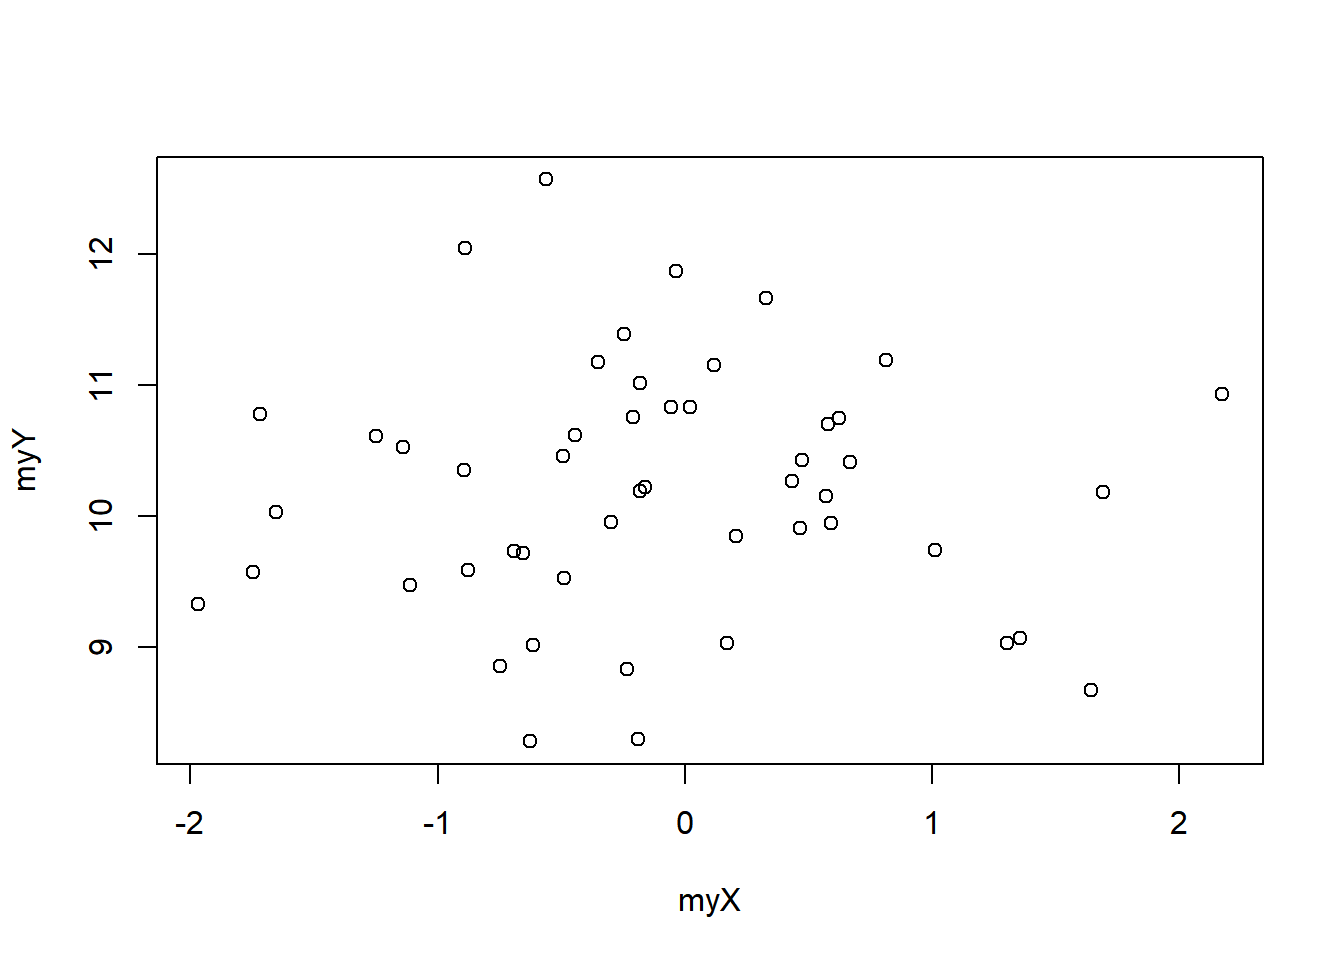
\includegraphics{myRBook_FR_files/figure-latex/unnamed-chunk-221-1.pdf}

Comme pour tous les types de graphiques, nous pouvons ajouter une légende sur l'axe des x et des y.

\begin{Shaded}
\begin{Highlighting}[]
\KeywordTok{plot}\NormalTok{(}\DataTypeTok{x =}\NormalTok{ myX, }\DataTypeTok{y =}\NormalTok{ myY, }
  \DataTypeTok{xlab =} \StringTok{"X"}\NormalTok{, }\DataTypeTok{ylab =} \StringTok{"Y"}\NormalTok{)}
\end{Highlighting}
\end{Shaded}

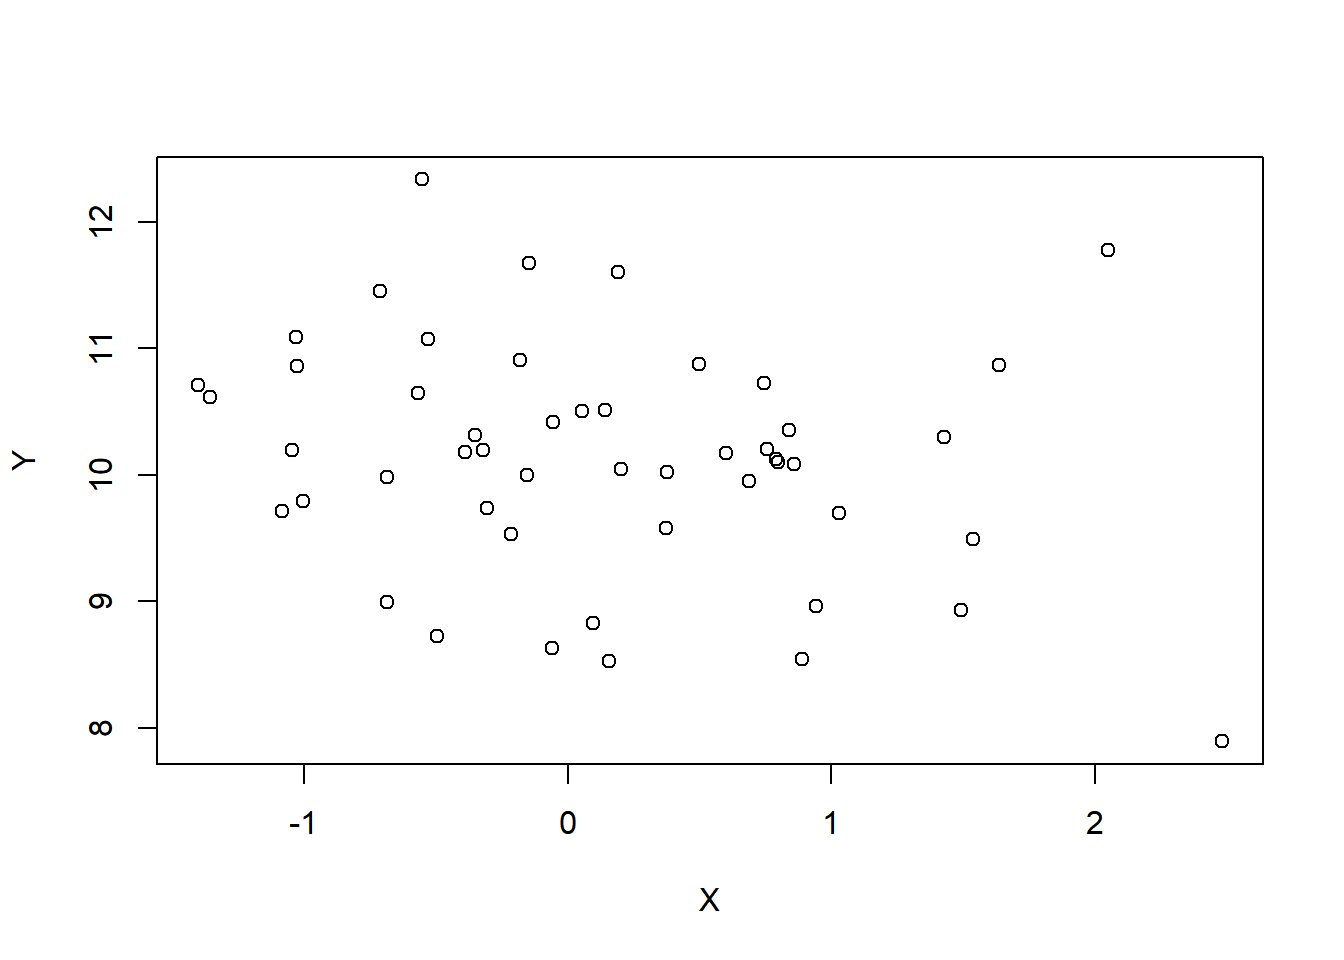
\includegraphics{myRBook_FR_files/figure-latex/unnamed-chunk-222-1.pdf}

Nous pouvons aussi définir les limites des axes en X et en Y.

\begin{Shaded}
\begin{Highlighting}[]
\KeywordTok{plot}\NormalTok{(}\DataTypeTok{x =}\NormalTok{ myX, }\DataTypeTok{y =}\NormalTok{ myY, }
  \DataTypeTok{xlab =} \StringTok{"X"}\NormalTok{, }\DataTypeTok{ylab =} \StringTok{"Y"}\NormalTok{, }
  \DataTypeTok{xlim =} \KeywordTok{c}\NormalTok{(}\OperatorTok{-}\DecValTok{3}\NormalTok{, }\DecValTok{3}\NormalTok{), }\DataTypeTok{ylim =} \KeywordTok{c}\NormalTok{(}\DecValTok{7}\NormalTok{, }\DecValTok{13}\NormalTok{))}
\end{Highlighting}
\end{Shaded}

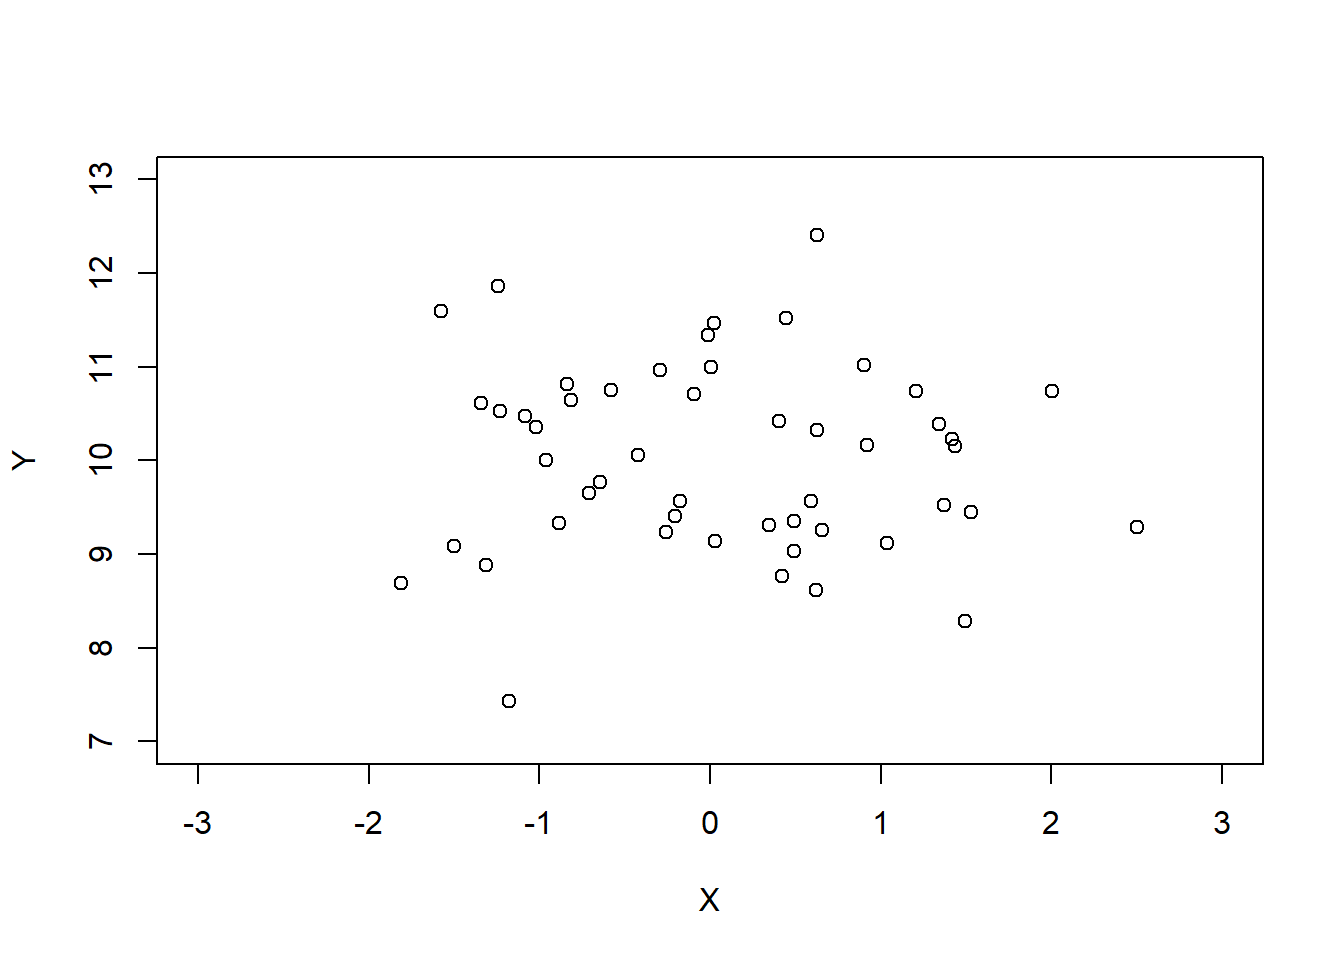
\includegraphics{myRBook_FR_files/figure-latex/unnamed-chunk-223-1.pdf}

Le type de point peut être défini avec l'argument \texttt{pch} qui peut prendre un caractère ou un chiffre de 1 à 25.

\begin{Shaded}
\begin{Highlighting}[]
\KeywordTok{plot}\NormalTok{(}\DataTypeTok{x =} \KeywordTok{rep}\NormalTok{(}\KeywordTok{seq}\NormalTok{(}\DecValTok{1}\OperatorTok{:}\DecValTok{5}\NormalTok{), }\DecValTok{5}\NormalTok{), }\DataTypeTok{y =} \KeywordTok{rep}\NormalTok{(}\KeywordTok{seq}\NormalTok{(}\DecValTok{1}\OperatorTok{:}\DecValTok{5}\NormalTok{), }\DataTypeTok{each =} \DecValTok{5}\NormalTok{),}
  \DataTypeTok{pch =} \DecValTok{1}\OperatorTok{:}\DecValTok{25}\NormalTok{)}
\end{Highlighting}
\end{Shaded}

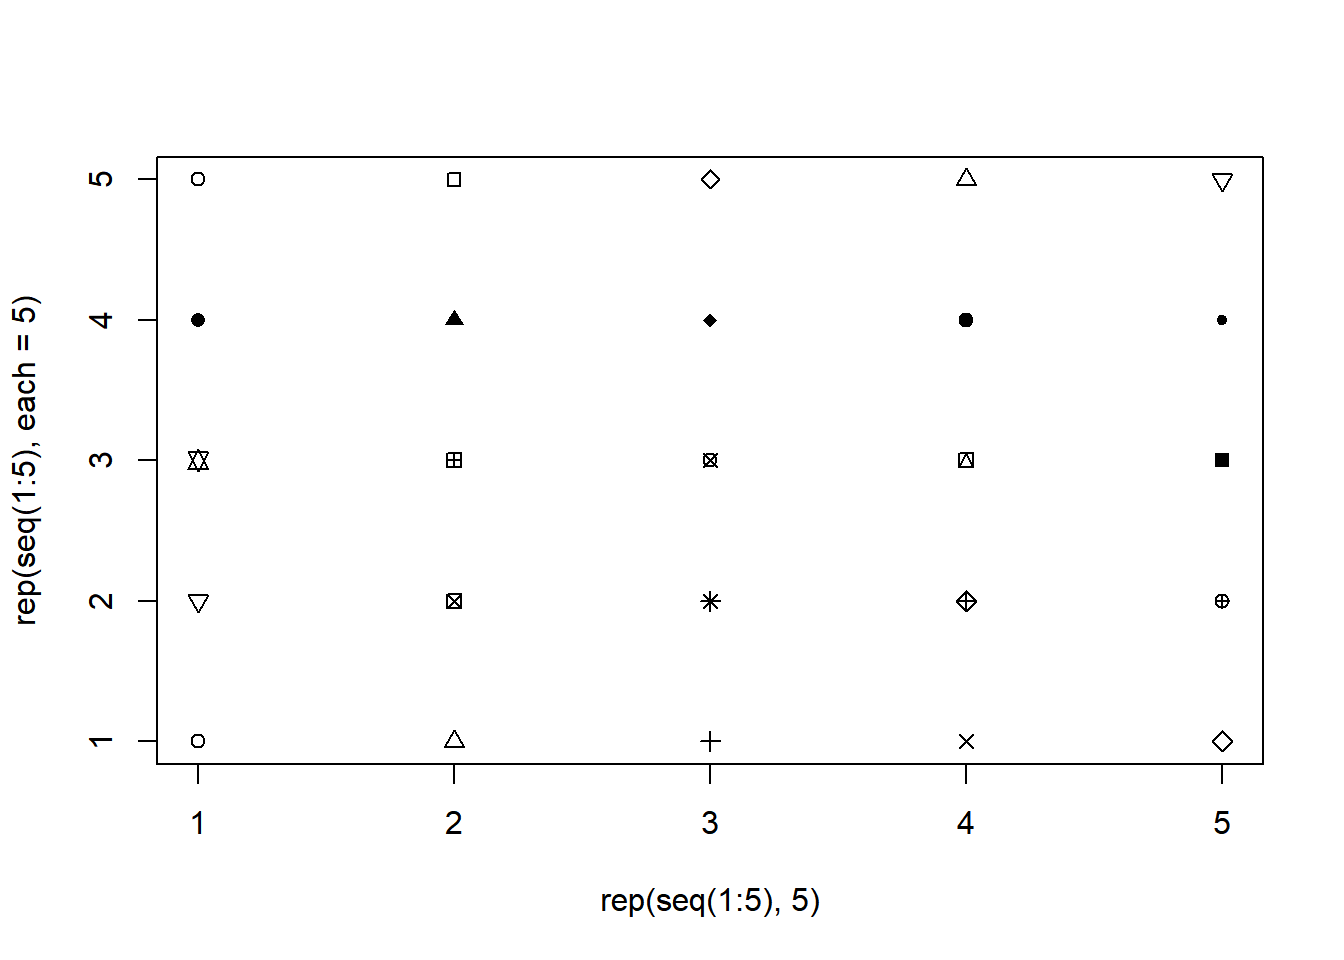
\includegraphics{myRBook_FR_files/figure-latex/unnamed-chunk-224-1.pdf}

\begin{Shaded}
\begin{Highlighting}[]
\KeywordTok{plot}\NormalTok{(}\DataTypeTok{x =}\NormalTok{ myX, }\DataTypeTok{y =}\NormalTok{ myY, }
  \DataTypeTok{pch =} \KeywordTok{c}\NormalTok{(}\StringTok{"a"}\NormalTok{, }\StringTok{"@"}\NormalTok{, }\StringTok{"#"}\NormalTok{, }\StringTok{"1"}\NormalTok{, }\StringTok{"="}\NormalTok{, }\StringTok{"-"}\NormalTok{, }\StringTok{"_"}\NormalTok{, }\StringTok{"o"}\NormalTok{, }\StringTok{"O"}\NormalTok{, }\StringTok{"0"}\NormalTok{, letters[}\DecValTok{1}\OperatorTok{:}\DecValTok{15}\NormalTok{]))}
\end{Highlighting}
\end{Shaded}

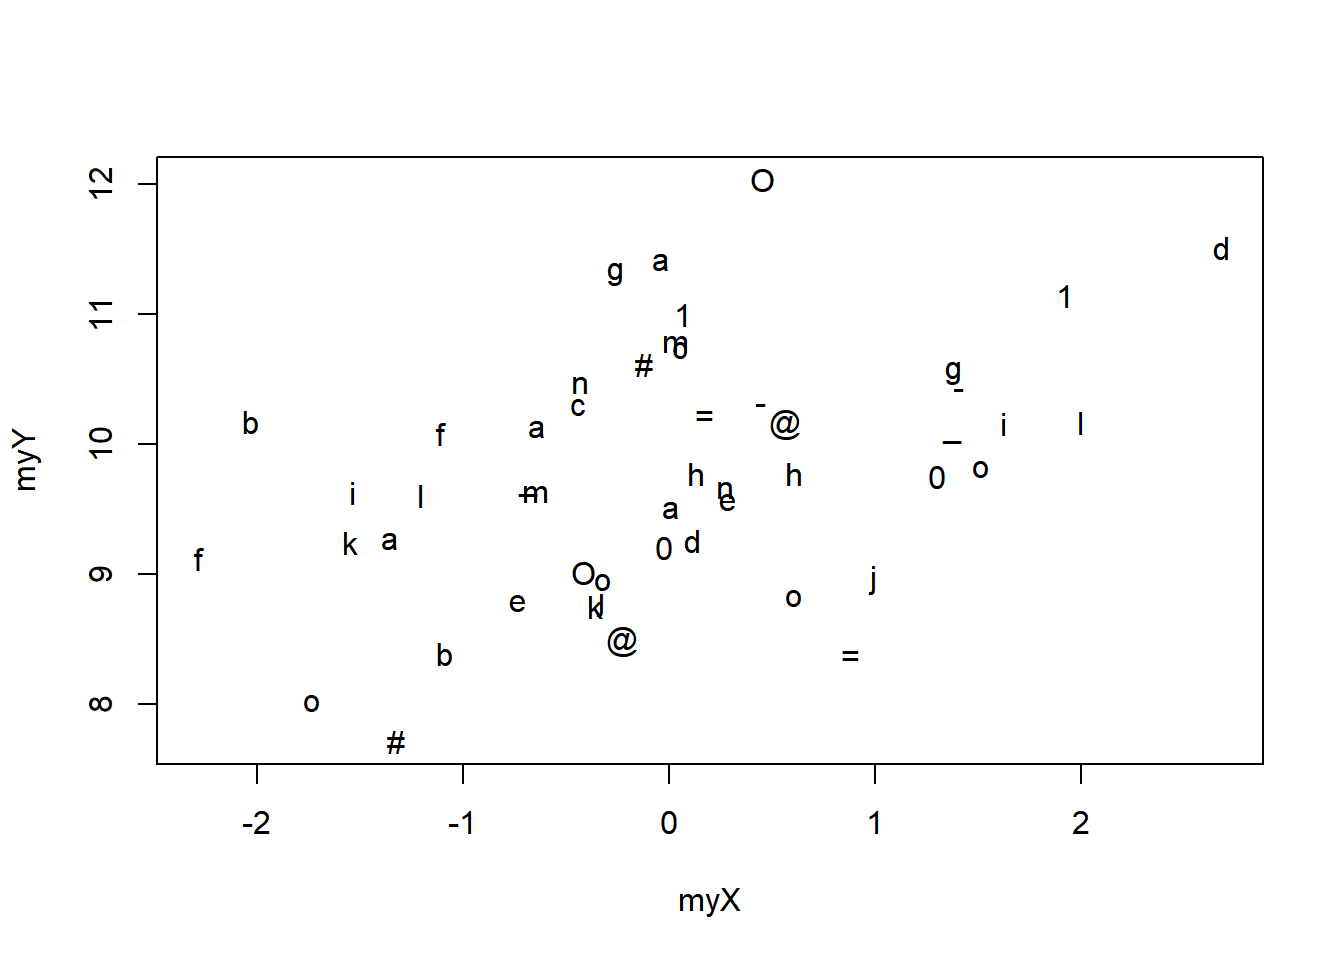
\includegraphics{myRBook_FR_files/figure-latex/unnamed-chunk-224-2.pdf}

La taille des points peut se définir avec l'argument \texttt{cex}.

\begin{Shaded}
\begin{Highlighting}[]
\KeywordTok{plot}\NormalTok{(}\DataTypeTok{x =}\NormalTok{ myX, }\DataTypeTok{y =}\NormalTok{ myY, }
  \DataTypeTok{cex =} \KeywordTok{seq}\NormalTok{(}\DataTypeTok{from =} \FloatTok{0.5}\NormalTok{, }\DataTypeTok{to =} \DecValTok{3}\NormalTok{, }\DataTypeTok{length.out =} \DecValTok{50}\NormalTok{))}
\end{Highlighting}
\end{Shaded}

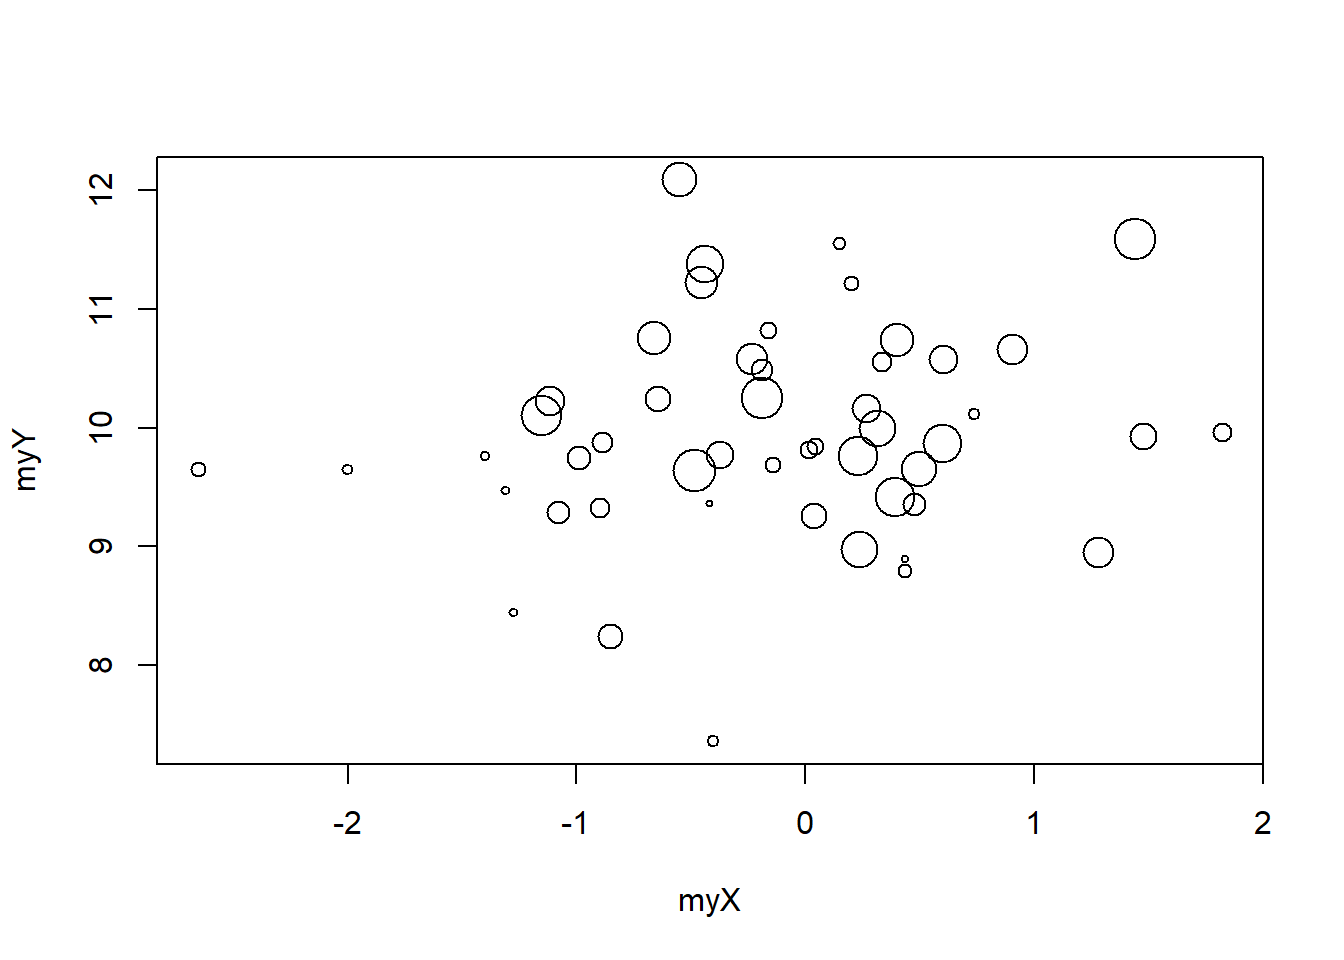
\includegraphics{myRBook_FR_files/figure-latex/unnamed-chunk-225-1.pdf}

La couleur des points peut se définir avec l'argument \texttt{col}. Nous reviendrons sur les couleurs dans un prochain chapitre.

\begin{Shaded}
\begin{Highlighting}[]
\NormalTok{myX <-}\StringTok{ }\KeywordTok{rnorm}\NormalTok{(}\DecValTok{100}\NormalTok{, }\DataTypeTok{mean =} \DecValTok{0}\NormalTok{, }\DataTypeTok{sd =} \DecValTok{1}\NormalTok{)}
\NormalTok{myY <-}\StringTok{ }\KeywordTok{rnorm}\NormalTok{(}\DecValTok{100}\NormalTok{, }\DataTypeTok{mean =} \DecValTok{10}\NormalTok{, }\DataTypeTok{sd =} \DecValTok{1}\NormalTok{)}
\KeywordTok{plot}\NormalTok{(}\DataTypeTok{x =}\NormalTok{ myX, }\DataTypeTok{y =}\NormalTok{ myY, }
  \DataTypeTok{cex =} \KeywordTok{seq}\NormalTok{(}\DataTypeTok{from =} \FloatTok{0.5}\NormalTok{, }\DataTypeTok{to =} \DecValTok{3}\NormalTok{, }\DataTypeTok{length.out =} \DecValTok{100}\NormalTok{),}
  \DataTypeTok{pch =} \DecValTok{16}\NormalTok{,}
  \DataTypeTok{col =} \KeywordTok{sample}\NormalTok{(}\KeywordTok{colors}\NormalTok{(), }\DecValTok{100}\NormalTok{))}
\end{Highlighting}
\end{Shaded}

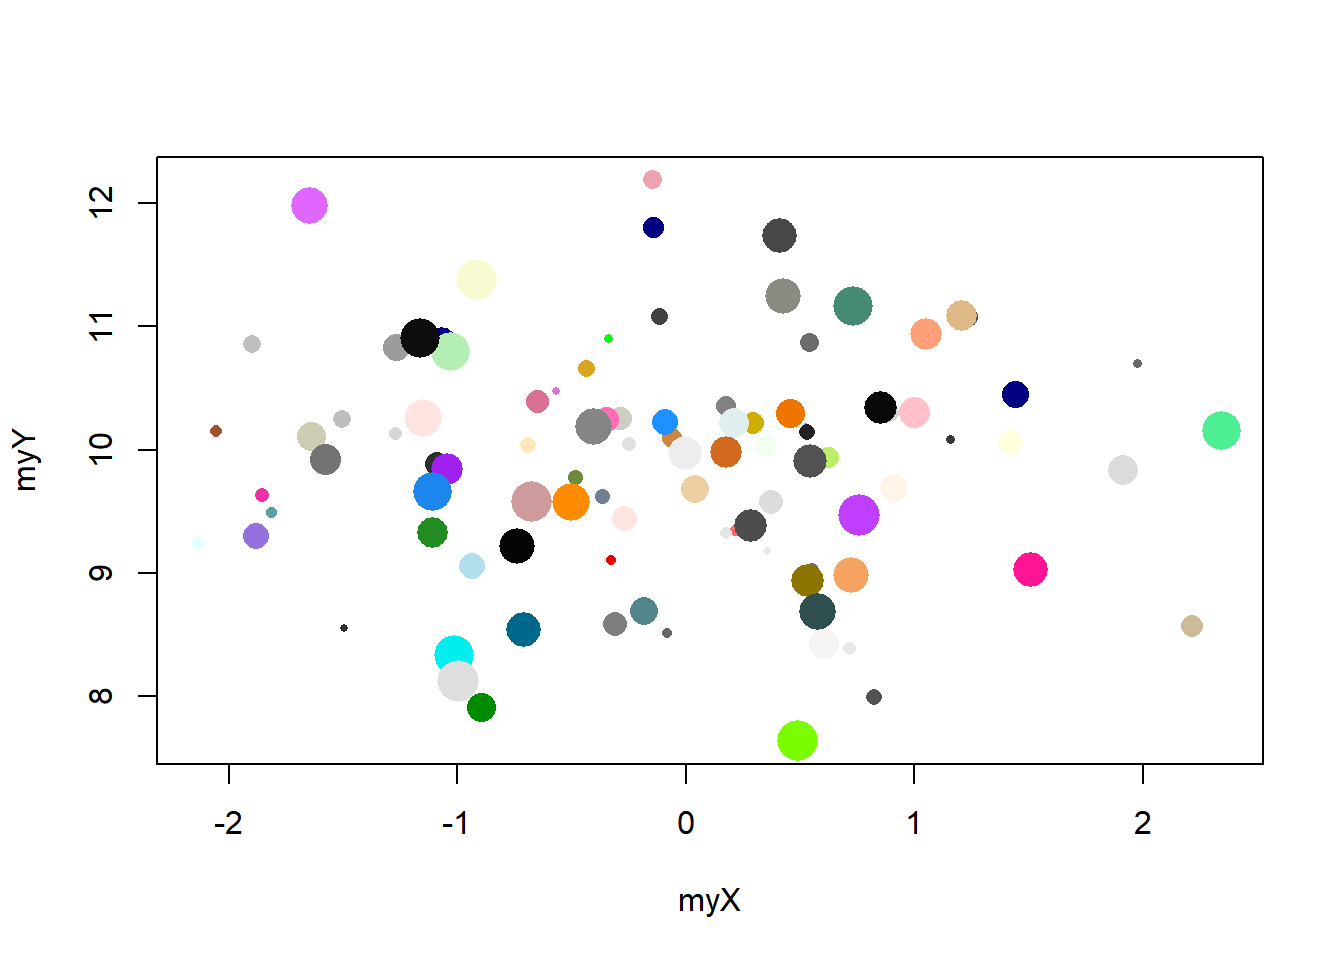
\includegraphics{myRBook_FR_files/figure-latex/unnamed-chunk-226-1.pdf}

Pour représenter nos points la couleur et la taille des points peuvent représenter des informations complémentaires. Ici nous allons représenter par un gradient de taille la variable \texttt{myY} et par un gradient de couleur la variable \texttt{myX}.

\begin{Shaded}
\begin{Highlighting}[]
\NormalTok{myX <-}\StringTok{ }\KeywordTok{rnorm}\NormalTok{(}\DecValTok{100}\NormalTok{)}
\NormalTok{myY <-}\StringTok{ }\KeywordTok{rnorm}\NormalTok{(}\DecValTok{100}\NormalTok{)}
\NormalTok{dfGraph <-}\StringTok{ }\KeywordTok{data.frame}\NormalTok{(myX, myY)}
\NormalTok{dfGraph <-}\StringTok{ }\NormalTok{dfGraph[}\KeywordTok{order}\NormalTok{(dfGraph}\OperatorTok{$}\NormalTok{myX),]}
\NormalTok{dfGraph}\OperatorTok{$}\NormalTok{myCol <-}\StringTok{ }\KeywordTok{colorRampPalette}\NormalTok{(}\KeywordTok{c}\NormalTok{(}\StringTok{"blue"}\NormalTok{, }\StringTok{"red"}\NormalTok{))(}\DecValTok{100}\NormalTok{)}
\NormalTok{dfGraph <-}\StringTok{ }\NormalTok{dfGraph[}\KeywordTok{order}\NormalTok{(dfGraph}\OperatorTok{$}\NormalTok{myY),]}
\NormalTok{dfGraph}\OperatorTok{$}\NormalTok{myCex <-}\StringTok{ }\KeywordTok{seq}\NormalTok{(}\DataTypeTok{from =} \FloatTok{0.5}\NormalTok{, }\DataTypeTok{to =} \DecValTok{3}\NormalTok{, }\DataTypeTok{length.out =} \DecValTok{100}\NormalTok{)}
\KeywordTok{plot}\NormalTok{(}\DataTypeTok{x =}\NormalTok{ dfGraph}\OperatorTok{$}\NormalTok{myX, }\DataTypeTok{y =}\NormalTok{ dfGraph}\OperatorTok{$}\NormalTok{myY, }
  \DataTypeTok{cex =}\NormalTok{ dfGraph}\OperatorTok{$}\NormalTok{myCex, }\DataTypeTok{pch =} \DecValTok{16}\NormalTok{, }\DataTypeTok{col =}\NormalTok{ dfGraph}\OperatorTok{$}\NormalTok{myCol, }
  \DataTypeTok{xlab =} \StringTok{""}\NormalTok{, }\DataTypeTok{ylab =} \StringTok{""}\NormalTok{)}
\end{Highlighting}
\end{Shaded}

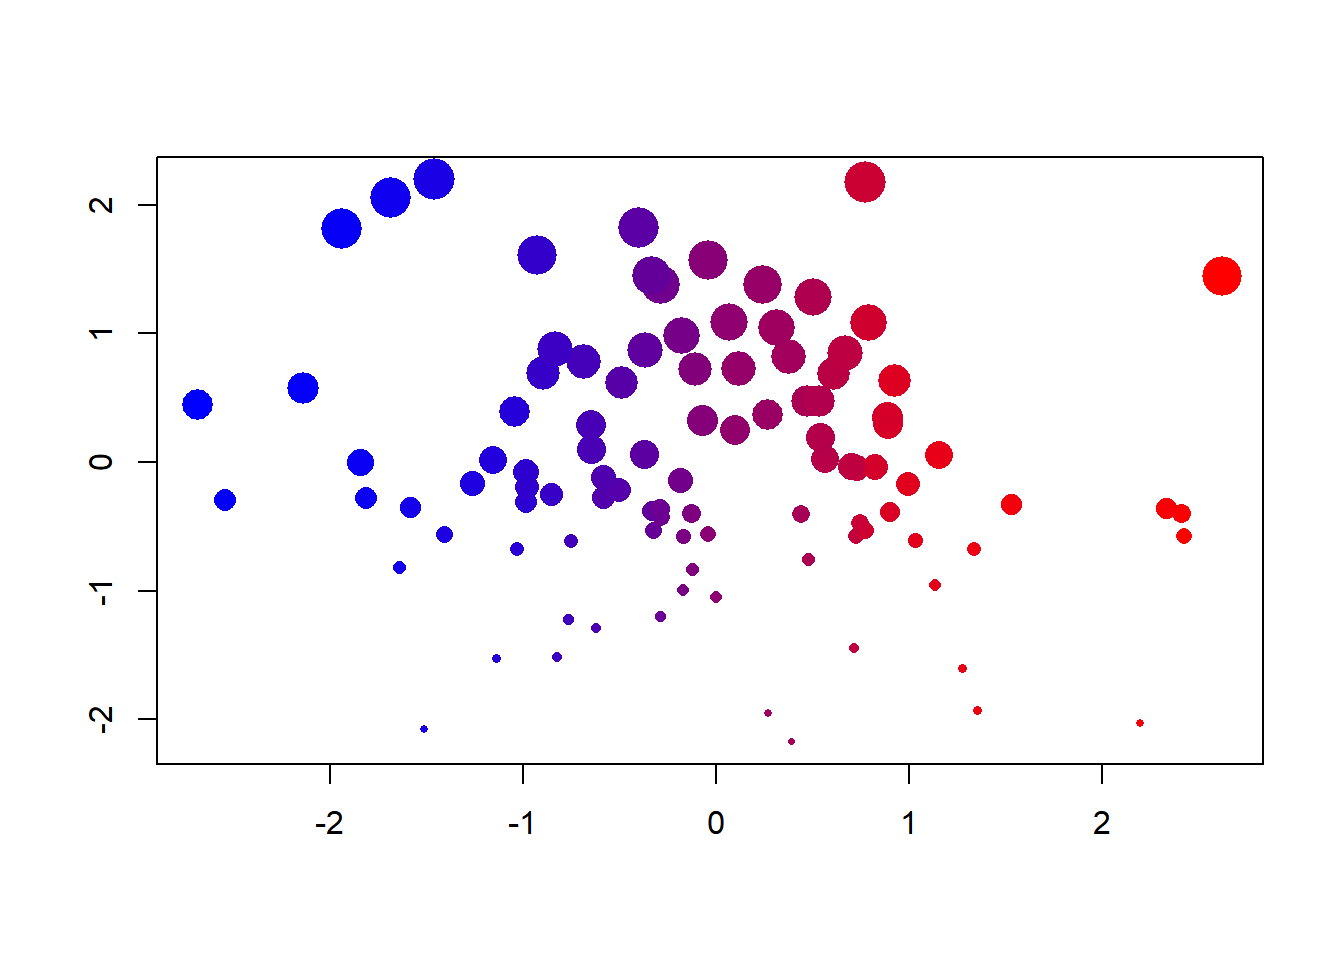
\includegraphics{myRBook_FR_files/figure-latex/unnamed-chunk-227-1.pdf}

R offre la possibilité de relier les points des nuages de points de différentes façons. Les différentes options sont disponibles dans l'aide de la fonction \texttt{plot()} et \texttt{plot.default()}.

\begin{Shaded}
\begin{Highlighting}[]
\NormalTok{myX <-}\StringTok{ }\DecValTok{1}\OperatorTok{:}\DecValTok{20}
\NormalTok{myY <-}\StringTok{ }\KeywordTok{rnorm}\NormalTok{(}\DecValTok{20}\NormalTok{, }\DataTypeTok{mean =} \DecValTok{10}\NormalTok{, }\DataTypeTok{sd =} \DecValTok{1}\NormalTok{)}
\KeywordTok{plot}\NormalTok{(}\DataTypeTok{x =}\NormalTok{ myX, }\DataTypeTok{y =}\NormalTok{ myY, }
  \DataTypeTok{type =} \StringTok{'b'}\NormalTok{) }\CommentTok{# 'p', 'l', 'b', 'c', 'o', 'h', 's', 'S', 'n'}
\end{Highlighting}
\end{Shaded}

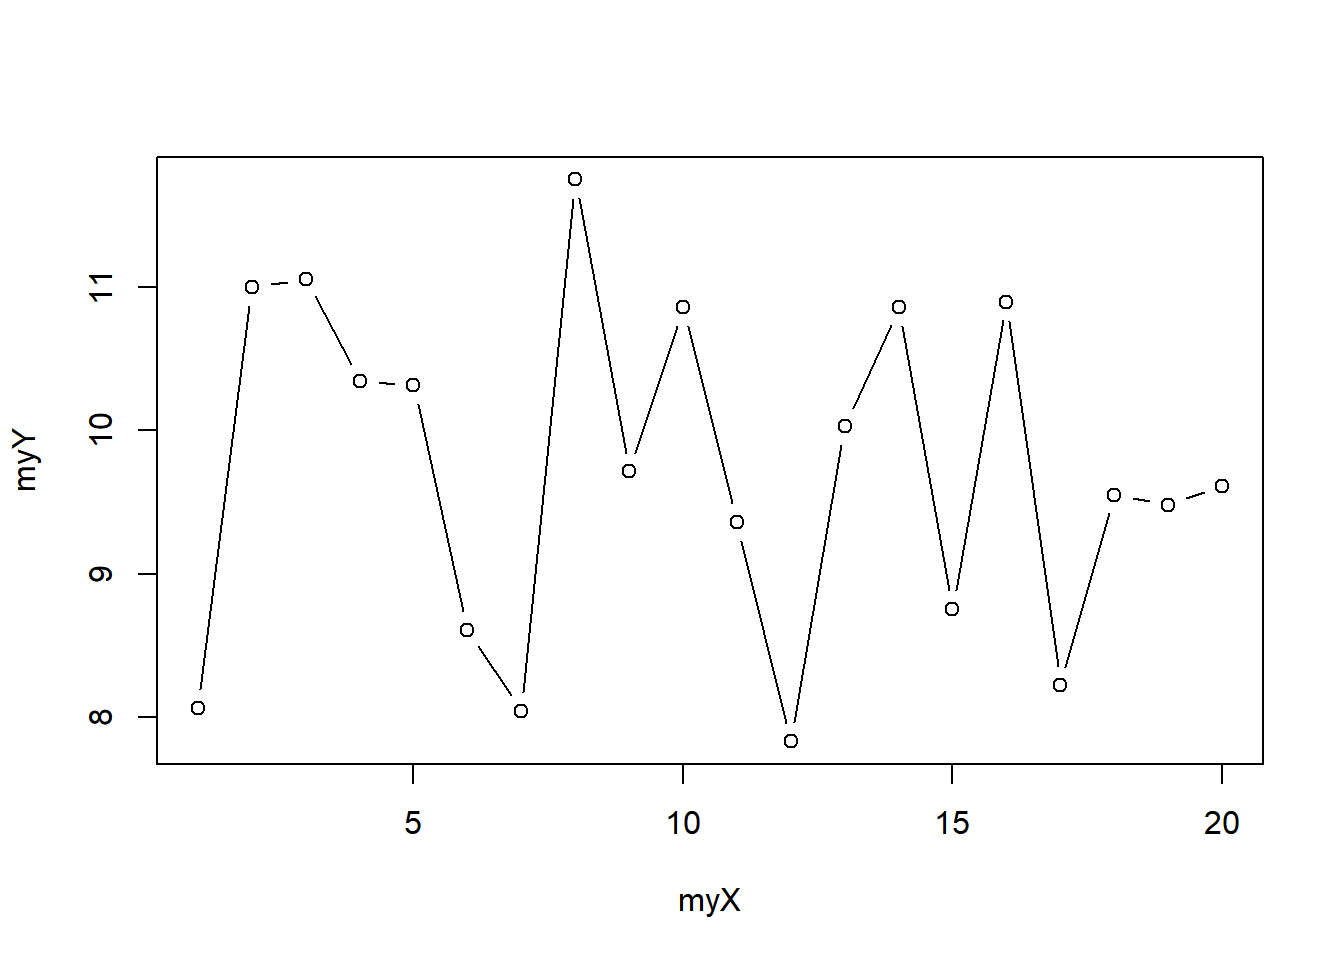
\includegraphics{myRBook_FR_files/figure-latex/unnamed-chunk-228-1.pdf}

Une dernière option très utile est l'argument \texttt{panel.first} qui permet de réaliser une opération graphique sur une couche située en dessous de notre graphique. Voici un exemple illustratif avec une grille réalisée avec et sans \texttt{panel.first}. La grille se fait grâce à la fonction \texttt{grid()}. Pour mettre les graphiques côte à côte nous allons utiliser \texttt{mfrow}.

\begin{Shaded}
\begin{Highlighting}[]
\KeywordTok{par}\NormalTok{(}\DataTypeTok{mfrow =} \KeywordTok{c}\NormalTok{(}\DecValTok{1}\NormalTok{, }\DecValTok{2}\NormalTok{))}
\KeywordTok{plot}\NormalTok{(}\DataTypeTok{x =}\NormalTok{ myX, }\DataTypeTok{y =}\NormalTok{ myY, }
  \DataTypeTok{type =} \StringTok{'b'}\NormalTok{, }\DataTypeTok{pch =} \DecValTok{16}\NormalTok{, }\DataTypeTok{cex =} \DecValTok{3}\NormalTok{) }
\KeywordTok{grid}\NormalTok{(}\DataTypeTok{lwd =} \DecValTok{3}\NormalTok{, }\DataTypeTok{lty =} \DecValTok{1}\NormalTok{)}
\KeywordTok{plot}\NormalTok{(}\DataTypeTok{x =}\NormalTok{ myX, }\DataTypeTok{y =}\NormalTok{ myY, }
  \DataTypeTok{type =} \StringTok{'b'}\NormalTok{, }\DataTypeTok{pch =} \DecValTok{16}\NormalTok{, }\DataTypeTok{cex =} \DecValTok{3}\NormalTok{, }
  \DataTypeTok{panel.first =} \KeywordTok{grid}\NormalTok{(}\DataTypeTok{lwd =} \DecValTok{3}\NormalTok{, }\DataTypeTok{lty =} \DecValTok{1}\NormalTok{)) }
\end{Highlighting}
\end{Shaded}

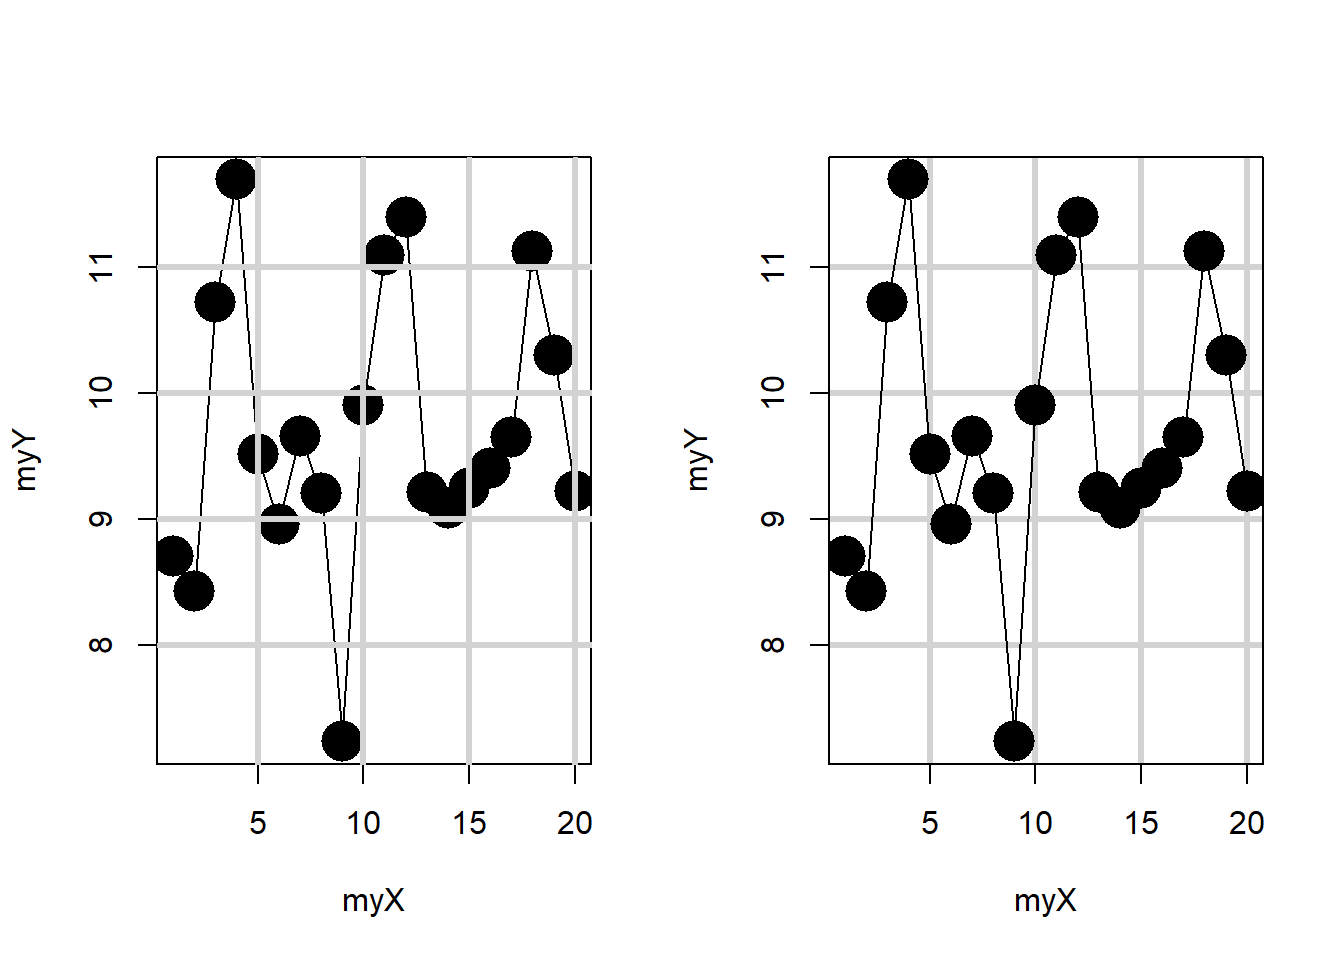
\includegraphics{myRBook_FR_files/figure-latex/unnamed-chunk-229-1.pdf}

\begin{Shaded}
\begin{Highlighting}[]
\KeywordTok{par}\NormalTok{(}\DataTypeTok{mfrow =} \KeywordTok{c}\NormalTok{(}\DecValTok{1}\NormalTok{, }\DecValTok{1}\NormalTok{))}
\end{Highlighting}
\end{Shaded}

La fonction \texttt{par()} permet d'accéder aux paramètres graphiques. Parmi ces paramètres il y a \texttt{mfrow} qui permet de diviser l'espace graphique comme une matrice. \texttt{mfrow} prend comme arguments un vecteur numérique de taille 2 : le premier élément correspond au nombre de lignes et le deuxième élément au nombre de colonnes. Le paramètre \texttt{mar} permet de contrôler les marges en bas, à gauche, en haut et à droite, respectivement, au moyen d'un vecteur numérique de taille 4. Après avoir modifié les paramètres graphiques par défaut il est recommandé de les réinitialiser pour que cela n'affecte pas les graphiques à venir. Les valeurs par défaut de \texttt{mfrow} sont \texttt{c(1,\ 1)} et \texttt{mar\ =\ c(4,\ 4,\ 4,\ 4)}. Nous pouvons remettre ces valeurs par défaut comme ci-dessus en redéfinissant chacun des paramètres. Nous pouvons également enregistrer au préalable les valeurs courantes (dans un objet \texttt{op}), puis les modifier pour les besoins de nos graphiques, puis ensuite rappeler les valeurs contenues dans l'objet \texttt{op}. Ici nous utilisons \texttt{lapply} pour réaliser rapidement quatre graphiques.

\begin{Shaded}
\begin{Highlighting}[]
\NormalTok{op <-}\StringTok{ }\KeywordTok{par}\NormalTok{(}\DataTypeTok{no.readonly =} \OtherTok{TRUE}\NormalTok{)}
\KeywordTok{par}\NormalTok{(}\DataTypeTok{mfrow =} \KeywordTok{c}\NormalTok{(}\DecValTok{2}\NormalTok{, }\DecValTok{2}\NormalTok{), }\DataTypeTok{mar =} \KeywordTok{c}\NormalTok{(}\DecValTok{2}\NormalTok{, }\DecValTok{2}\NormalTok{, }\DecValTok{1}\NormalTok{, }\DecValTok{1}\NormalTok{))}
\NormalTok{graph4 <-}\StringTok{ }\KeywordTok{lapply}\NormalTok{(}\DecValTok{1}\OperatorTok{:}\DecValTok{4}\NormalTok{, }\ControlFlowTok{function}\NormalTok{(i)\{}
  \KeywordTok{plot}\NormalTok{(}\DataTypeTok{x =} \KeywordTok{rnorm}\NormalTok{(}\DecValTok{100}\NormalTok{), }
    \DataTypeTok{y =} \KeywordTok{rnorm}\NormalTok{(}\DecValTok{100}\NormalTok{), }
    \DataTypeTok{col =}\NormalTok{ i, }\DataTypeTok{pch =} \DecValTok{16}\NormalTok{)}
\NormalTok{\})}
\end{Highlighting}
\end{Shaded}

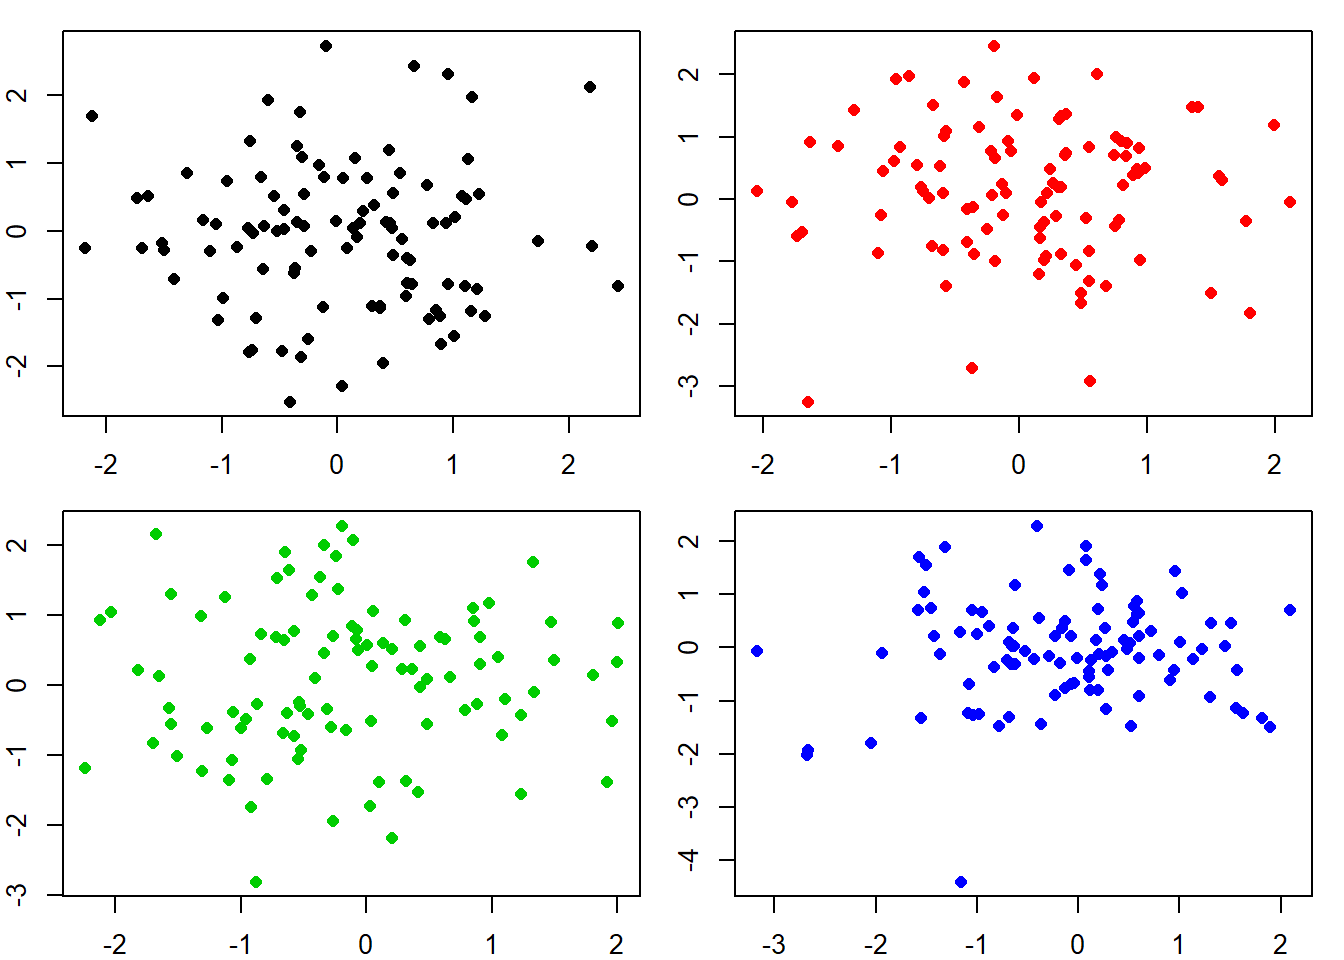
\includegraphics{myRBook_FR_files/figure-latex/unnamed-chunk-230-1.pdf}

\begin{Shaded}
\begin{Highlighting}[]
\KeywordTok{par}\NormalTok{(op)}
\end{Highlighting}
\end{Shaded}

Il est souvent utile de faire figurer des lignes verticales ou horizontales pour représenter des valeurs particulières. Ces lignes peuvent être ajoutées avec la fonction \texttt{abline()}.

\begin{Shaded}
\begin{Highlighting}[]
\NormalTok{myX <-}\StringTok{ }\KeywordTok{rnorm}\NormalTok{(}\DecValTok{100}\NormalTok{)}
\NormalTok{myY <-}\StringTok{ }\KeywordTok{rnorm}\NormalTok{(}\DecValTok{100}\NormalTok{)}
\KeywordTok{plot}\NormalTok{(}\DataTypeTok{x =}\NormalTok{ myX, }\DataTypeTok{y =}\NormalTok{ myY, }
  \DataTypeTok{xlim =} \KeywordTok{c}\NormalTok{(}\OperatorTok{-}\DecValTok{4}\NormalTok{, }\DecValTok{4}\NormalTok{), }\DataTypeTok{ylim =} \KeywordTok{c}\NormalTok{(}\OperatorTok{-}\DecValTok{4}\NormalTok{, }\DecValTok{4}\NormalTok{),   }
  \DataTypeTok{pch =} \DecValTok{16}\NormalTok{, }\DataTypeTok{cex =} \FloatTok{1.5}\NormalTok{, }
  \DataTypeTok{col =} \KeywordTok{sample}\NormalTok{(}\KeywordTok{colors}\NormalTok{(), }\DataTypeTok{size =} \DecValTok{100}\NormalTok{),}
  \DataTypeTok{panel.first =}\NormalTok{ \{}
    \KeywordTok{grid}\NormalTok{()}
    \KeywordTok{abline}\NormalTok{(}\DataTypeTok{v =} \KeywordTok{c}\NormalTok{(}\KeywordTok{min}\NormalTok{(myX), }\KeywordTok{max}\NormalTok{(myX)), }\DataTypeTok{lty =} \DecValTok{2}\NormalTok{)}
    \KeywordTok{abline}\NormalTok{(}\DataTypeTok{h =} \KeywordTok{c}\NormalTok{(}\KeywordTok{min}\NormalTok{(myY), }\KeywordTok{max}\NormalTok{(myY)), }\DataTypeTok{lty =} \DecValTok{2}\NormalTok{)}
    \KeywordTok{abline}\NormalTok{(}\DataTypeTok{v =} \KeywordTok{mean}\NormalTok{(myX), }\DataTypeTok{lty =} \DecValTok{1}\NormalTok{)}
    \KeywordTok{abline}\NormalTok{(}\DataTypeTok{h =} \KeywordTok{mean}\NormalTok{(myY), }\DataTypeTok{lty =} \DecValTok{1}\NormalTok{)}
\NormalTok{\})}
\end{Highlighting}
\end{Shaded}

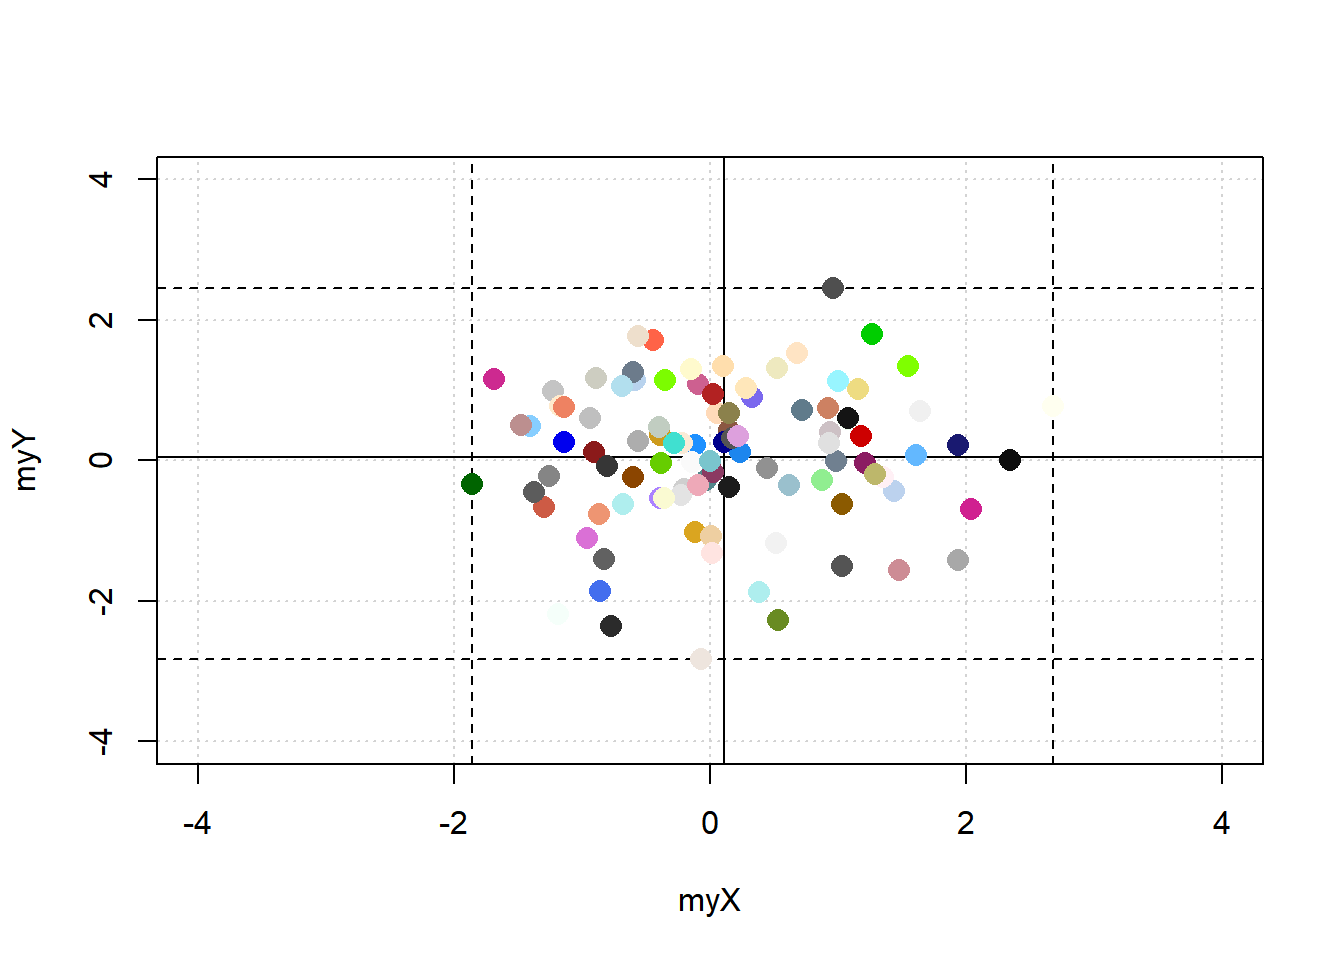
\includegraphics{myRBook_FR_files/figure-latex/unnamed-chunk-231-1.pdf}

\hypertarget{graph1hist}{%
\section{\texorpdfstring{\texttt{hist}}{hist}}\label{graph1hist}}

Pour faire un histogramme nous utilisons la fonction \texttt{hist()}. C'est une fonction graphique utile pour visualiser rapidement la distribution d'un jeu de données.

\begin{Shaded}
\begin{Highlighting}[]
\NormalTok{op <-}\StringTok{ }\KeywordTok{par}\NormalTok{(}\DataTypeTok{no.readonly =} \OtherTok{TRUE}\NormalTok{)}
\KeywordTok{par}\NormalTok{(}\DataTypeTok{mfrow =} \KeywordTok{c}\NormalTok{(}\DecValTok{2}\NormalTok{, }\DecValTok{2}\NormalTok{), }\DataTypeTok{mar =} \KeywordTok{c}\NormalTok{(}\DecValTok{2}\NormalTok{, }\DecValTok{2}\NormalTok{, }\DecValTok{1}\NormalTok{, }\DecValTok{1}\NormalTok{))}
\NormalTok{myX <-}\StringTok{ }\KeywordTok{list}\NormalTok{(}
  \KeywordTok{rnorm}\NormalTok{(}\DecValTok{1000}\NormalTok{),}
  \KeywordTok{rgamma}\NormalTok{(}\DecValTok{1000}\NormalTok{, }\DataTypeTok{shape =} \DecValTok{1}\NormalTok{),}
  \KeywordTok{sample}\NormalTok{(}\DecValTok{1}\OperatorTok{:}\DecValTok{100}\NormalTok{, }\DataTypeTok{size =} \DecValTok{1000}\NormalTok{, }\DataTypeTok{replace =} \OtherTok{TRUE}\NormalTok{),}
  \KeywordTok{rbeta}\NormalTok{(}\DecValTok{1000}\NormalTok{, }\DataTypeTok{shape1 =} \DecValTok{1}\NormalTok{, }\DataTypeTok{shape2 =} \DecValTok{2}\NormalTok{)}
\NormalTok{)}
\NormalTok{myTitle <-}\StringTok{ }\KeywordTok{c}\NormalTok{(}\StringTok{"Normal"}\NormalTok{, }\StringTok{"Gamma"}\NormalTok{, }\StringTok{"Uniform"}\NormalTok{, }\StringTok{"Beta"}\NormalTok{)}
\NormalTok{tr <-}\StringTok{ }\KeywordTok{lapply}\NormalTok{(}\DecValTok{1}\OperatorTok{:}\DecValTok{4}\NormalTok{, }\ControlFlowTok{function}\NormalTok{(i)\{}
  \KeywordTok{hist}\NormalTok{(myX[[i]], }
    \DataTypeTok{col =} \KeywordTok{heat.colors}\NormalTok{(}\DecValTok{15}\NormalTok{), }
    \DataTypeTok{main =}\NormalTok{ myTitle[i]}
\NormalTok{  )}
\NormalTok{\})}
\end{Highlighting}
\end{Shaded}

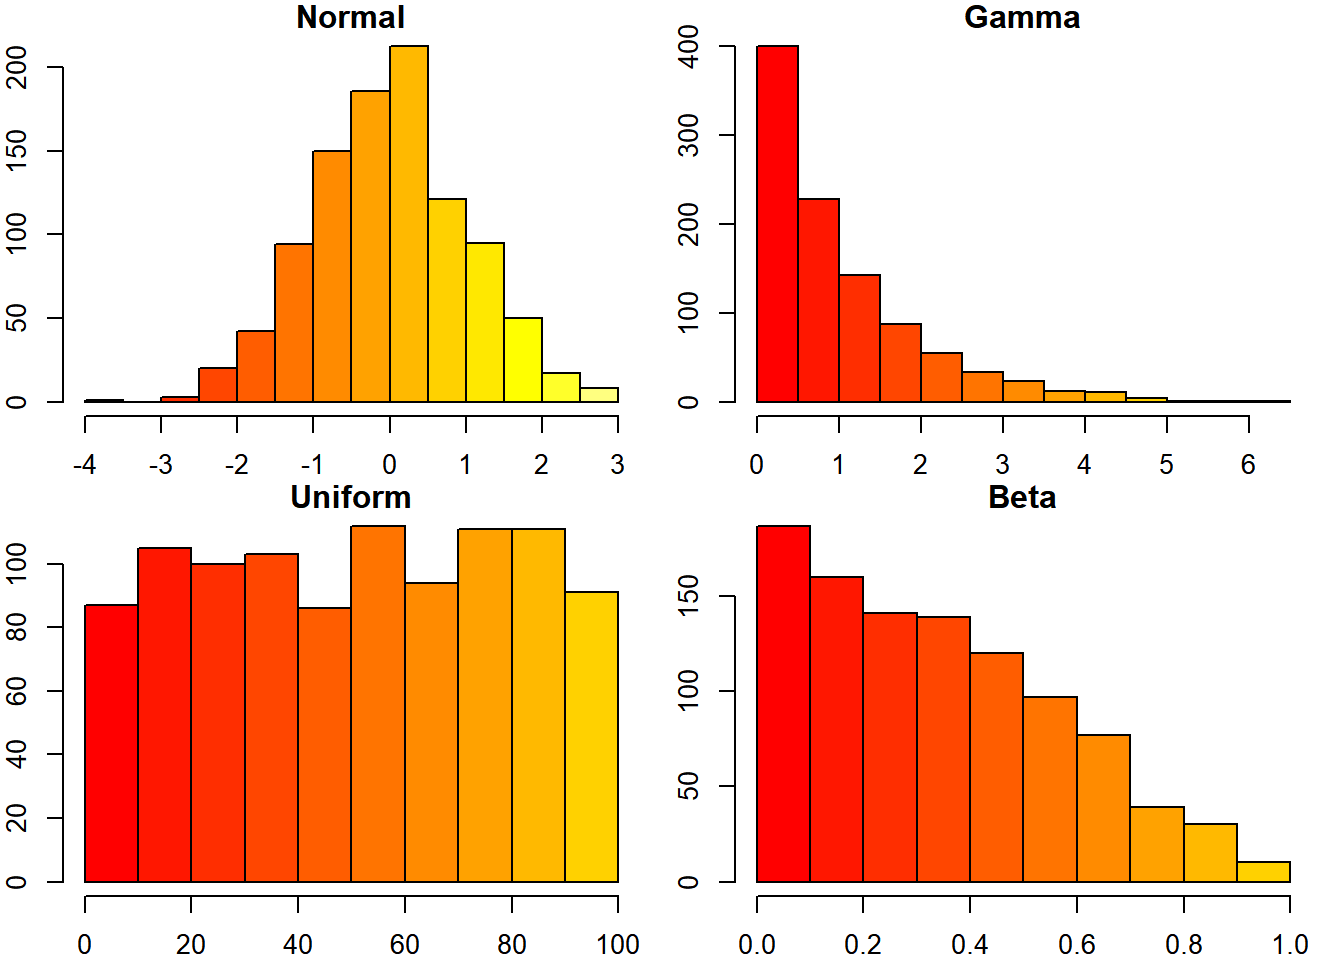
\includegraphics{myRBook_FR_files/figure-latex/unnamed-chunk-232-1.pdf}

\begin{Shaded}
\begin{Highlighting}[]
\KeywordTok{par}\NormalTok{(op)}
\end{Highlighting}
\end{Shaded}

\hypertarget{graph1barplot}{%
\section{\texorpdfstring{\texttt{barplot}}{barplot}}\label{graph1barplot}}

Le graphique en barres se fait au moyen de la fonction \texttt{barplot()}.

\begin{Shaded}
\begin{Highlighting}[]
\NormalTok{myX <-}\StringTok{ }\KeywordTok{c}\NormalTok{(}\DecValTok{4}\NormalTok{, }\DecValTok{5}\NormalTok{, }\DecValTok{8}\NormalTok{)}
\KeywordTok{barplot}\NormalTok{(myX, }\DataTypeTok{names.arg =} \KeywordTok{c}\NormalTok{(}\StringTok{"A"}\NormalTok{, }\StringTok{"B"}\NormalTok{, }\StringTok{"C"}\NormalTok{))}
\end{Highlighting}
\end{Shaded}

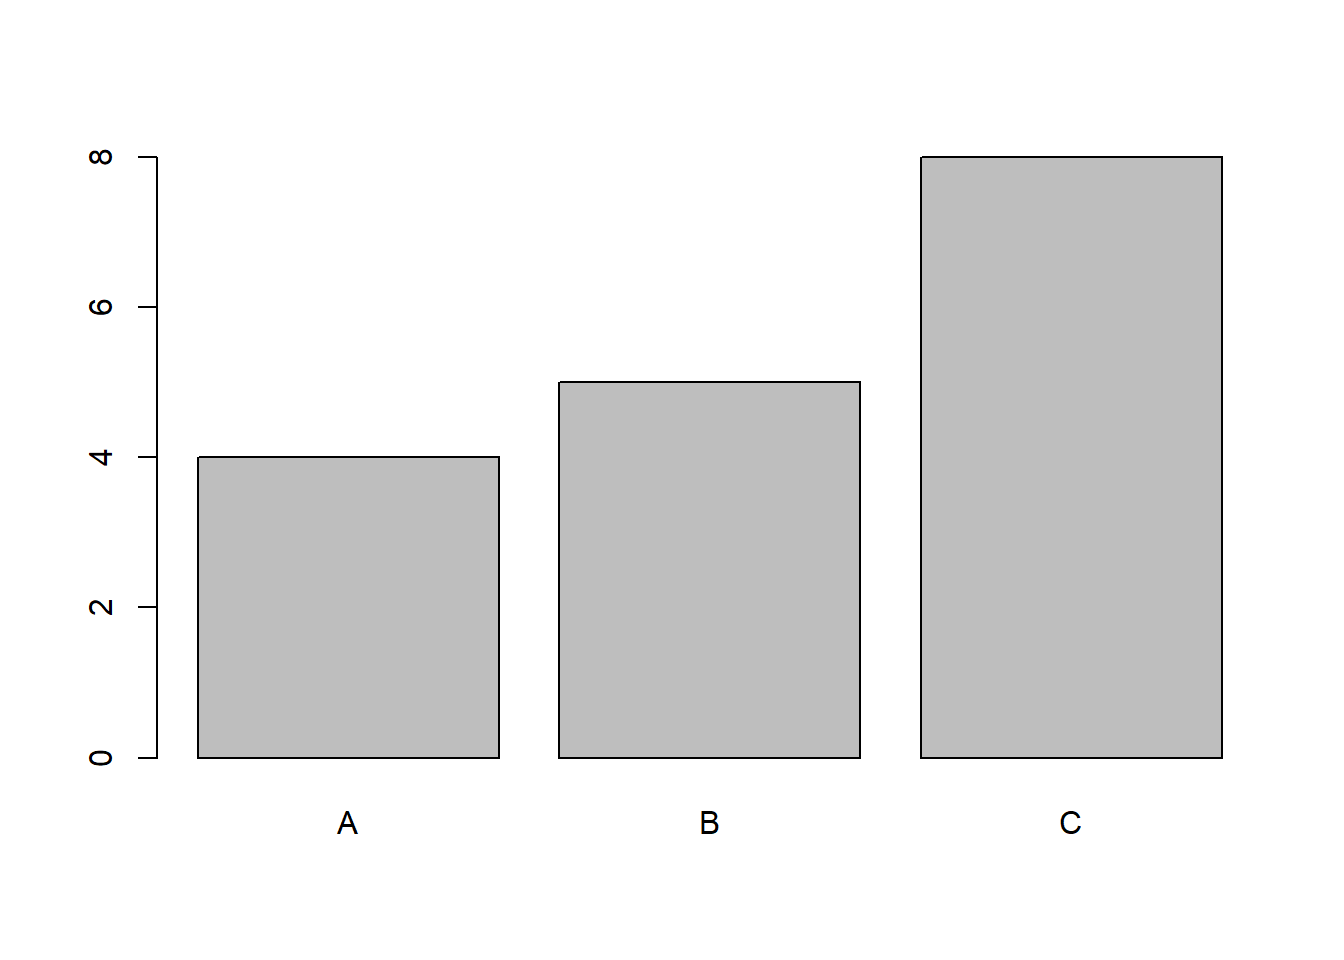
\includegraphics{myRBook_FR_files/figure-latex/unnamed-chunk-233-1.pdf}

Quand l'objet envoyé à cette fonction est un \texttt{vector} alors la fonction \texttt{barplot()} renvoie un graphique en barres simples. Quand c'est une \texttt{matrix} alors les barres sont multiples.

\begin{Shaded}
\begin{Highlighting}[]
\NormalTok{op <-}\StringTok{ }\KeywordTok{par}\NormalTok{(}\DataTypeTok{no.readonly =} \OtherTok{TRUE}\NormalTok{)}
\KeywordTok{par}\NormalTok{(}\DataTypeTok{mfrow =} \KeywordTok{c}\NormalTok{(}\DecValTok{1}\NormalTok{, }\DecValTok{2}\NormalTok{), }\DataTypeTok{mar =} \KeywordTok{c}\NormalTok{(}\DecValTok{2}\NormalTok{, }\DecValTok{2}\NormalTok{, }\DecValTok{1}\NormalTok{, }\DecValTok{1}\NormalTok{))}
\NormalTok{myX <-}\StringTok{ }\KeywordTok{matrix}\NormalTok{(}\KeywordTok{c}\NormalTok{(}\DecValTok{4}\NormalTok{, }\DecValTok{5}\NormalTok{, }\DecValTok{8}\NormalTok{, }\DecValTok{4}\NormalTok{, }\DecValTok{6}\NormalTok{, }\DecValTok{2}\NormalTok{), }\DataTypeTok{nrow =} \DecValTok{2}\NormalTok{)}
\KeywordTok{barplot}\NormalTok{(myX, }\DataTypeTok{names.arg =} \KeywordTok{c}\NormalTok{(}\StringTok{"A"}\NormalTok{, }\StringTok{"B"}\NormalTok{, }\StringTok{"C"}\NormalTok{))}
\NormalTok{myX <-}\StringTok{ }\KeywordTok{matrix}\NormalTok{(}\KeywordTok{c}\NormalTok{(}\DecValTok{4}\NormalTok{, }\DecValTok{5}\NormalTok{, }\DecValTok{8}\NormalTok{, }\DecValTok{4}\NormalTok{, }\DecValTok{6}\NormalTok{, }\DecValTok{2}\NormalTok{, }\DecValTok{3}\NormalTok{, }\DecValTok{4}\NormalTok{, }\DecValTok{5}\NormalTok{), }\DataTypeTok{nrow =} \DecValTok{3}\NormalTok{)}
\KeywordTok{barplot}\NormalTok{(myX, }\DataTypeTok{names.arg =} \KeywordTok{c}\NormalTok{(}\StringTok{"A"}\NormalTok{, }\StringTok{"B"}\NormalTok{, }\StringTok{"C"}\NormalTok{))}
\end{Highlighting}
\end{Shaded}

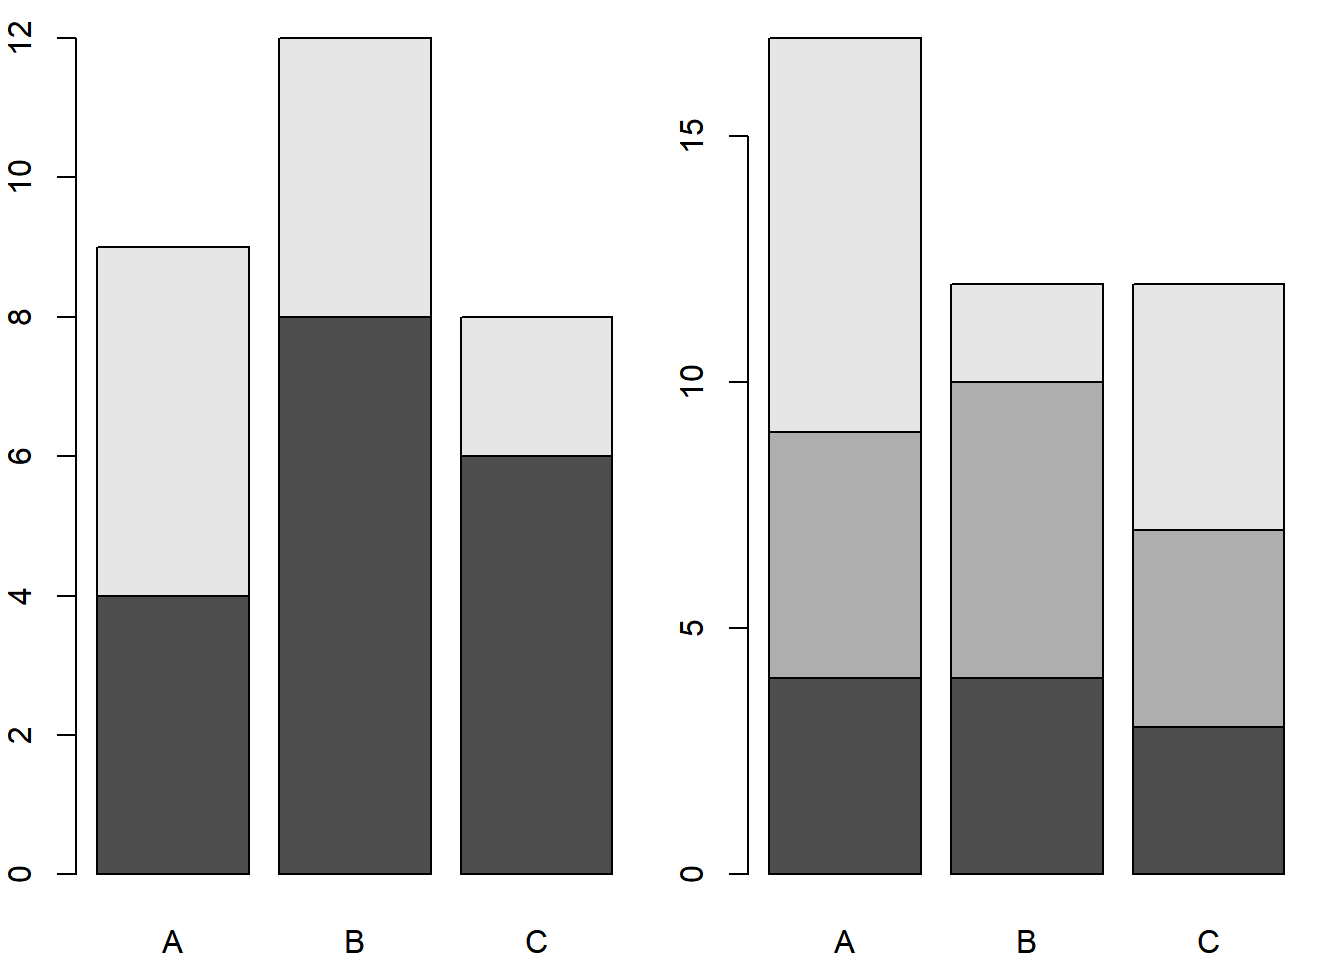
\includegraphics{myRBook_FR_files/figure-latex/unnamed-chunk-234-1.pdf}

\begin{Shaded}
\begin{Highlighting}[]
\KeywordTok{par}\NormalTok{(op)}
\end{Highlighting}
\end{Shaded}

La fonction \texttt{barplot()} peut aussi être utilisée pour représenter l'équivalent d'un histogramme. Cela peut être utile pour représenter la distribution d'une variable en fonction de l'axe des abscisses et l'axe des ordonnées. Dans l'exemple qui suit nous avons \texttt{n} points tirés au hasard dans une loi normale de paramètres \texttt{mean\ =\ 0} et \texttt{sd\ =\ 1} (\texttt{myX\ \textless{}-\ rnorm(n)}). Ces points sont soit représentés en bleu, soit représentés en rouge (la couleur bleue est codée avec la valeur 4 et la couleur rouge avec la valeur 2, nous en reparlerons dans un prochain chapitre). Le tirage au hasard de la couleur se fait avec la fonction \texttt{sample()} (\texttt{myCol\ \textless{}-\ sample(c(4,\ 2),\ size\ =\ n,\ replace\ =\ TRUE)}). Ici nous voulons représenter un nuage de points avec les points en rouge ou en bleu, puis pour l'axe des abscisses et l'axe des ordonnées, des histogrammes pour voir la répartition des points et un gradient de couleur du bleu au rouge en fonction de la proportion des points de couleur dans chaque catégorie. Le gradient de couleur avec 100 valeurs entre bleu et rouge se réalise avec la fonction \texttt{colorRampPalette()} (\texttt{myColors\ \textless{}-\ colorRampPalette(c("blue",\ "red"))(100)}).

Pour faire l'histogramme nous allons découper les données avec la fonction \texttt{cut()} en spécifiant que nous souhaitons des séparations faites entre -4 et 4 par pas de 1 (\texttt{myYCut\ \textless{}-\ cut(myY,\ breaks\ =\ -4:4)}). Pour avoir le compte du nombre de points dans chacune des catégories et pour chaque couleur il nous suffit d'utiliser la fonction \texttt{table()} (\texttt{myYCutCol\ \textless{}-\ table(myCol,\ myYCut)}). Dans cette table la première ligne correspond à la première couleur rencontrée dans le jeu de données et la deuxième ligne à l'autre couleur. C'est pourquoi il nous faut modifier le tirage aléatoire des couleurs pour que la première ligne corresponde toujours au bleu et la deuxième ligne au rouge : \texttt{myCol\ \textless{}-\ c(2,\ sample(c(4,\ 2),\ size\ =\ (n\ -\ 1),\ replace\ =\ TRUE))}.

Ensuite nous pouvons calculer la proportion de rouge en divisant la première ligne par la somme des deux lignes que nous allons représenter en pourcentage en multipliant par 100 : \texttt{myXCutCol{[}1,{]}\ /\ (myXCutCol{[}1,{]}\ +\ myXCutCol{[}2,{]})\ *\ 100}. Pour que ce chiffre corresponde à une couleur nous n'allons conserver que sa partie entière avec la fonction \texttt{round()}. Si le pourcentage est de zéro ou si le résultat n'est pas possible du fait d'une division par zéro alors il nous faut le remplacer par 1 afin que cela corresponde à une couleur dans notre gradient qui va de 1 à 100 (\texttt{xCol{[}is.na(xCol)\ \textbar{}\ xCol\ ==\ 0{]}\ \textless{}-\ 1}).

Il ne nous reste plus qu'à organiser l'espace graphique avec la fonction \texttt{layout()} qui prend comme argument une matrice dont les valeurs et leur position vont correspondre à l'agencement des différents graphiques que nous souhaitons réaliser. Le graphique 1 correspond au barplot du haut, le graphique 2 au nuage de points et le graphique 3 au barplot de droite.

\begin{Shaded}
\begin{Highlighting}[]
\NormalTok{n <-}\StringTok{ }\DecValTok{50}
\NormalTok{myX <-}\StringTok{ }\KeywordTok{rnorm}\NormalTok{(n)}
\NormalTok{myY <-}\StringTok{ }\KeywordTok{rnorm}\NormalTok{(n)}
\NormalTok{myCol <-}\StringTok{ }\KeywordTok{c}\NormalTok{(}\DecValTok{2}\NormalTok{, }\KeywordTok{sample}\NormalTok{(}\KeywordTok{c}\NormalTok{(}\DecValTok{4}\NormalTok{, }\DecValTok{2}\NormalTok{), }\DataTypeTok{size =}\NormalTok{ (n }\OperatorTok{-}\StringTok{ }\DecValTok{1}\NormalTok{), }\DataTypeTok{replace =} \OtherTok{TRUE}\NormalTok{))}
\NormalTok{myColors <-}\StringTok{ }\KeywordTok{colorRampPalette}\NormalTok{(}\KeywordTok{c}\NormalTok{(}\StringTok{"blue"}\NormalTok{, }\StringTok{"red"}\NormalTok{))(}\DecValTok{100}\NormalTok{)}
\NormalTok{myYCut <-}\StringTok{ }\KeywordTok{cut}\NormalTok{(myY, }\DataTypeTok{breaks =} \DecValTok{-4}\OperatorTok{:}\DecValTok{4}\NormalTok{)}
\NormalTok{myXCut <-}\StringTok{ }\KeywordTok{cut}\NormalTok{(myX, }\DataTypeTok{breaks =} \DecValTok{-4}\OperatorTok{:}\DecValTok{4}\NormalTok{)}
\NormalTok{myYCutCol <-}\StringTok{ }\KeywordTok{table}\NormalTok{(myCol, myYCut)}
\NormalTok{myXCutCol <-}\StringTok{ }\KeywordTok{table}\NormalTok{(myCol, myXCut)}
\NormalTok{xCol <-}\StringTok{ }\KeywordTok{round}\NormalTok{(}
\NormalTok{  myXCutCol[}\DecValTok{1}\NormalTok{,] }\OperatorTok{/}\StringTok{ }\NormalTok{(myXCutCol[}\DecValTok{1}\NormalTok{,] }\OperatorTok{+}\StringTok{ }\NormalTok{myXCutCol[}\DecValTok{2}\NormalTok{,]) }\OperatorTok{*}\StringTok{ }\DecValTok{100}
\NormalTok{)}
\NormalTok{xCol[}\KeywordTok{is.na}\NormalTok{(xCol) }\OperatorTok{|}\StringTok{ }\NormalTok{xCol }\OperatorTok{==}\StringTok{ }\DecValTok{0}\NormalTok{] <-}\StringTok{ }\DecValTok{1}
\NormalTok{yCol <-}\StringTok{ }\KeywordTok{round}\NormalTok{(}
\NormalTok{  myYCutCol[}\DecValTok{1}\NormalTok{,] }\OperatorTok{/}\StringTok{ }\NormalTok{(myYCutCol[}\DecValTok{1}\NormalTok{,] }\OperatorTok{+}\StringTok{ }\NormalTok{myYCutCol[}\DecValTok{2}\NormalTok{,]) }\OperatorTok{*}\StringTok{ }\DecValTok{100}
\NormalTok{)}
\NormalTok{yCol[}\KeywordTok{is.na}\NormalTok{(yCol) }\OperatorTok{|}\StringTok{ }\NormalTok{yCol }\OperatorTok{==}\StringTok{ }\DecValTok{0}\NormalTok{] <-}\StringTok{ }\DecValTok{1}
\NormalTok{op <-}\StringTok{ }\KeywordTok{par}\NormalTok{(}\DataTypeTok{no.readonly =} \OtherTok{TRUE}\NormalTok{)}
\KeywordTok{par}\NormalTok{(}\DataTypeTok{mar =} \KeywordTok{c}\NormalTok{(}\DecValTok{2}\NormalTok{, }\DecValTok{3}\NormalTok{, }\DecValTok{1}\NormalTok{, }\DecValTok{1}\NormalTok{))}
\KeywordTok{layout}\NormalTok{(}\KeywordTok{matrix}\NormalTok{(}\KeywordTok{c}\NormalTok{(}\DecValTok{1}\NormalTok{, }\DecValTok{1}\NormalTok{, }\DecValTok{0}\NormalTok{, }
                \DecValTok{2}\NormalTok{, }\DecValTok{2}\NormalTok{, }\DecValTok{3}\NormalTok{, }
                \DecValTok{2}\NormalTok{, }\DecValTok{2}\NormalTok{, }\DecValTok{3}\NormalTok{), }\DataTypeTok{ncol =} \DecValTok{3}\NormalTok{, }\DataTypeTok{byrow =} \OtherTok{TRUE}\NormalTok{))}
\KeywordTok{barplot}\NormalTok{(}\KeywordTok{table}\NormalTok{(myXCut), }\DataTypeTok{las =} \DecValTok{1}\NormalTok{, }\DataTypeTok{col =}\NormalTok{ myColors[xCol])}
\KeywordTok{plot}\NormalTok{(}\DataTypeTok{x =}\NormalTok{ myX, }\DataTypeTok{y =}\NormalTok{ myY, }\DataTypeTok{col =}\NormalTok{ myCol, }\DataTypeTok{pch =} \DecValTok{16}\NormalTok{, }
  \DataTypeTok{xlim =} \KeywordTok{c}\NormalTok{(}\OperatorTok{-}\DecValTok{4}\NormalTok{, }\DecValTok{4}\NormalTok{), }\DataTypeTok{ylim =} \KeywordTok{c}\NormalTok{(}\OperatorTok{-}\DecValTok{4}\NormalTok{, }\DecValTok{4}\NormalTok{), }\DataTypeTok{cex =} \FloatTok{1.5}\NormalTok{, }
  \DataTypeTok{panel.first =} \KeywordTok{grid}\NormalTok{())}
\KeywordTok{barplot}\NormalTok{(}\KeywordTok{table}\NormalTok{(myYCut), }\DataTypeTok{las =} \DecValTok{1}\NormalTok{, }\DataTypeTok{horiz =} \OtherTok{TRUE}\NormalTok{, }\DataTypeTok{col =}\NormalTok{ myColors[yCol])}
\end{Highlighting}
\end{Shaded}

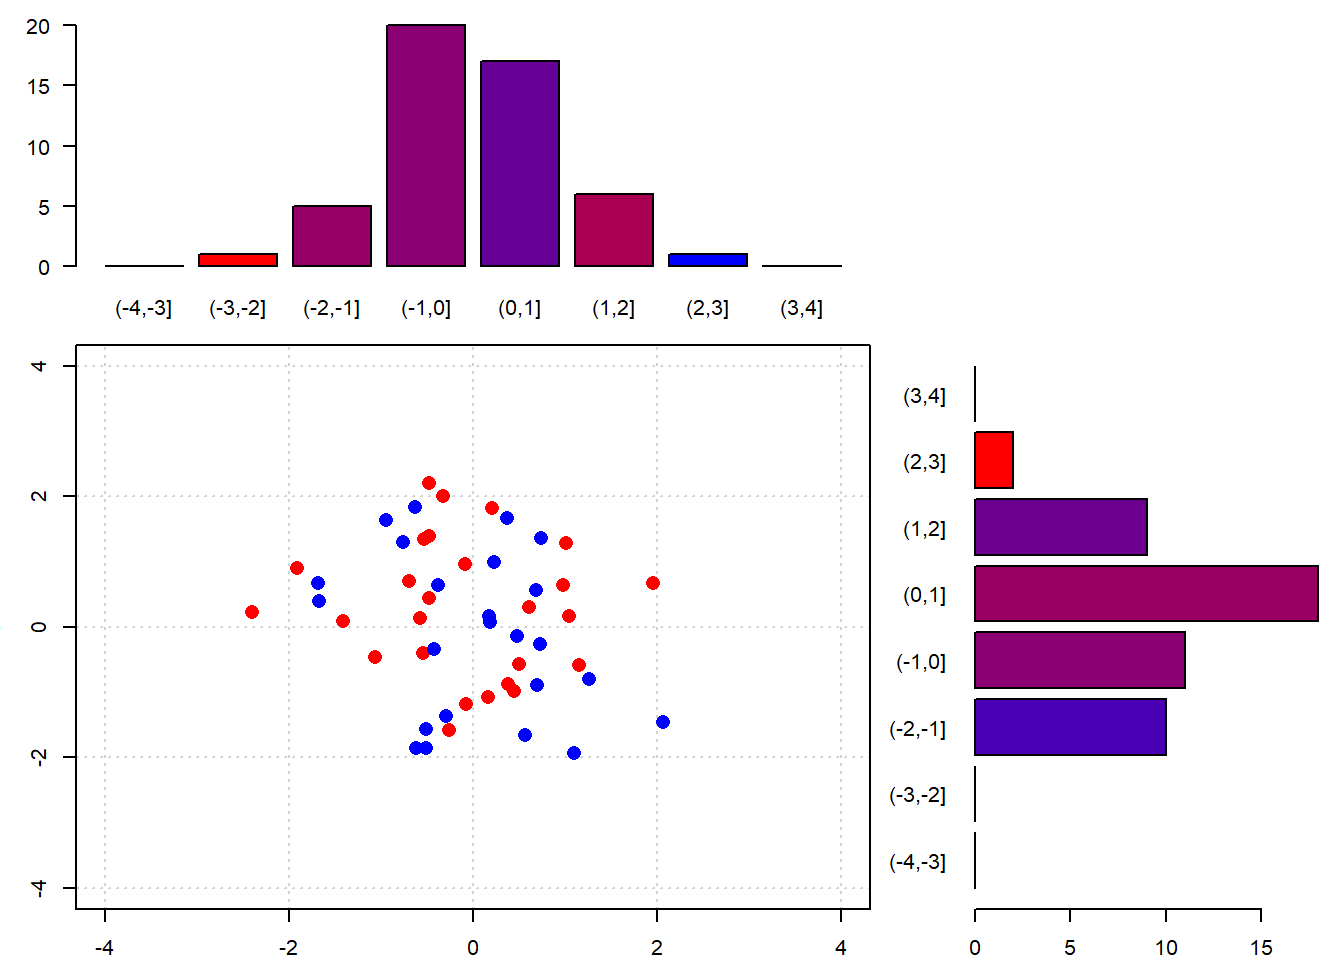
\includegraphics{myRBook_FR_files/figure-latex/unnamed-chunk-235-1.pdf}

\begin{Shaded}
\begin{Highlighting}[]
\KeywordTok{par}\NormalTok{(op)}
\end{Highlighting}
\end{Shaded}

Nous pouvons ensuite intégrer ce script dans une fonction pour par exemple étudier l'effet de la variable \texttt{n}.

\begin{Shaded}
\begin{Highlighting}[]
\NormalTok{graphBarplotCol <-}\StringTok{ }\ControlFlowTok{function}\NormalTok{(n)\{}
\NormalTok{  myX <-}\StringTok{ }\KeywordTok{rnorm}\NormalTok{(n)}
\NormalTok{  myY <-}\StringTok{ }\KeywordTok{rnorm}\NormalTok{(n)}
\NormalTok{  myCol <-}\StringTok{ }\KeywordTok{c}\NormalTok{(}\DecValTok{2}\NormalTok{, }\KeywordTok{sample}\NormalTok{(}\KeywordTok{c}\NormalTok{(}\DecValTok{4}\NormalTok{, }\DecValTok{2}\NormalTok{), }\DataTypeTok{size =}\NormalTok{ (n }\OperatorTok{-}\StringTok{ }\DecValTok{1}\NormalTok{), }\DataTypeTok{replace =} \OtherTok{TRUE}\NormalTok{))}
\NormalTok{  myColors <-}\StringTok{ }\KeywordTok{colorRampPalette}\NormalTok{(}\KeywordTok{c}\NormalTok{(}\StringTok{"blue"}\NormalTok{, }\StringTok{"red"}\NormalTok{))(}\DecValTok{100}\NormalTok{)}
\NormalTok{  myYCut <-}\StringTok{ }\KeywordTok{cut}\NormalTok{(myY, }\DataTypeTok{breaks =} \DecValTok{-4}\OperatorTok{:}\DecValTok{4}\NormalTok{)}
\NormalTok{  myXCut <-}\StringTok{ }\KeywordTok{cut}\NormalTok{(myX, }\DataTypeTok{breaks =} \DecValTok{-4}\OperatorTok{:}\DecValTok{4}\NormalTok{)}
\NormalTok{  myYCutCol <-}\StringTok{ }\KeywordTok{table}\NormalTok{(myCol, myYCut)}
\NormalTok{  myXCutCol <-}\StringTok{ }\KeywordTok{table}\NormalTok{(myCol, myXCut)}
\NormalTok{  xCol <-}\StringTok{ }\KeywordTok{round}\NormalTok{(}
\NormalTok{    myXCutCol[}\DecValTok{1}\NormalTok{,] }\OperatorTok{/}\StringTok{ }\NormalTok{(myXCutCol[}\DecValTok{1}\NormalTok{,] }\OperatorTok{+}\StringTok{ }\NormalTok{myXCutCol[}\DecValTok{2}\NormalTok{,]) }\OperatorTok{*}\StringTok{ }\DecValTok{100}
\NormalTok{  )}
\NormalTok{  xCol[}\KeywordTok{is.na}\NormalTok{(xCol) }\OperatorTok{|}\StringTok{ }\NormalTok{xCol }\OperatorTok{==}\StringTok{ }\DecValTok{0}\NormalTok{] <-}\StringTok{ }\DecValTok{1}
\NormalTok{  yCol <-}\StringTok{ }\KeywordTok{round}\NormalTok{(}
\NormalTok{    myYCutCol[}\DecValTok{1}\NormalTok{,] }\OperatorTok{/}\StringTok{ }\NormalTok{(myYCutCol[}\DecValTok{1}\NormalTok{,] }\OperatorTok{+}\StringTok{ }\NormalTok{myYCutCol[}\DecValTok{2}\NormalTok{,]) }\OperatorTok{*}\StringTok{ }\DecValTok{100}
\NormalTok{  )}
\NormalTok{  yCol[}\KeywordTok{is.na}\NormalTok{(yCol) }\OperatorTok{|}\StringTok{ }\NormalTok{yCol }\OperatorTok{==}\StringTok{ }\DecValTok{0}\NormalTok{] <-}\StringTok{ }\DecValTok{1}
\NormalTok{  op <-}\StringTok{ }\KeywordTok{par}\NormalTok{(}\DataTypeTok{no.readonly =} \OtherTok{TRUE}\NormalTok{)}
  \KeywordTok{par}\NormalTok{(}\DataTypeTok{mar =} \KeywordTok{c}\NormalTok{(}\DecValTok{2}\NormalTok{, }\DecValTok{3}\NormalTok{, }\DecValTok{1}\NormalTok{, }\DecValTok{1}\NormalTok{))}
  \KeywordTok{layout}\NormalTok{(}\KeywordTok{matrix}\NormalTok{(}\KeywordTok{c}\NormalTok{(}\DecValTok{1}\NormalTok{, }\DecValTok{1}\NormalTok{, }\DecValTok{0}\NormalTok{, }
                  \DecValTok{2}\NormalTok{, }\DecValTok{2}\NormalTok{, }\DecValTok{3}\NormalTok{, }
                  \DecValTok{2}\NormalTok{, }\DecValTok{2}\NormalTok{, }\DecValTok{3}\NormalTok{), }\DataTypeTok{ncol =} \DecValTok{3}\NormalTok{, }\DataTypeTok{byrow =} \OtherTok{TRUE}\NormalTok{))}
  \KeywordTok{barplot}\NormalTok{(}\KeywordTok{table}\NormalTok{(myXCut), }\DataTypeTok{las =} \DecValTok{1}\NormalTok{, }\DataTypeTok{col =}\NormalTok{ myColors[xCol])}
  \KeywordTok{plot}\NormalTok{(}\DataTypeTok{x =}\NormalTok{ myX, }\DataTypeTok{y =}\NormalTok{ myY, }\DataTypeTok{col =}\NormalTok{ myCol, }\DataTypeTok{pch =} \DecValTok{16}\NormalTok{, }
    \DataTypeTok{xlim =} \KeywordTok{c}\NormalTok{(}\OperatorTok{-}\DecValTok{4}\NormalTok{, }\DecValTok{4}\NormalTok{), }\DataTypeTok{ylim =} \KeywordTok{c}\NormalTok{(}\OperatorTok{-}\DecValTok{4}\NormalTok{, }\DecValTok{4}\NormalTok{), }\DataTypeTok{cex =} \FloatTok{1.5}\NormalTok{, }
    \DataTypeTok{panel.first =} \KeywordTok{grid}\NormalTok{())}
  \KeywordTok{barplot}\NormalTok{(}\KeywordTok{table}\NormalTok{(myYCut), }\DataTypeTok{las =} \DecValTok{1}\NormalTok{, }\DataTypeTok{horiz =} \OtherTok{TRUE}\NormalTok{, }\DataTypeTok{col =}\NormalTok{ myColors[yCol])}
  \KeywordTok{par}\NormalTok{(op)}
\NormalTok{\}}
\KeywordTok{graphBarplotCol}\NormalTok{(}\DataTypeTok{n =} \DecValTok{1000}\NormalTok{)}
\end{Highlighting}
\end{Shaded}

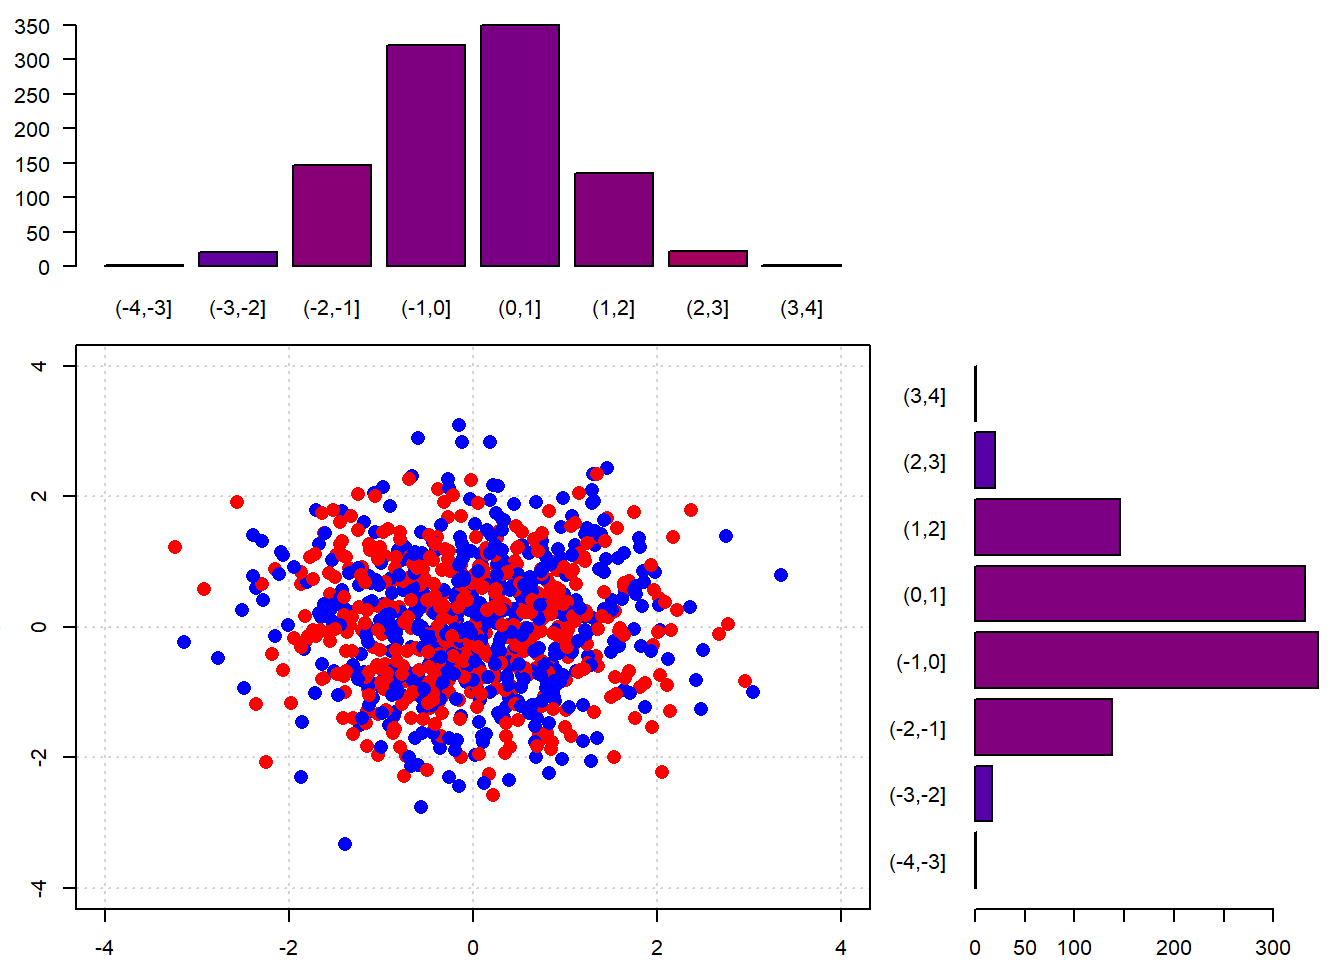
\includegraphics{myRBook_FR_files/figure-latex/unnamed-chunk-236-1.pdf}

Un \texttt{barplot} peut bien sûr prendre des valeurs positives ou négatives.

\begin{Shaded}
\begin{Highlighting}[]
\KeywordTok{barplot}\NormalTok{(}\KeywordTok{rnorm}\NormalTok{(}\DecValTok{20}\NormalTok{), }\DataTypeTok{horiz =} \OtherTok{TRUE}\NormalTok{, }\DataTypeTok{col =} \KeywordTok{rainbow}\NormalTok{(}\DecValTok{20}\NormalTok{))}
\end{Highlighting}
\end{Shaded}

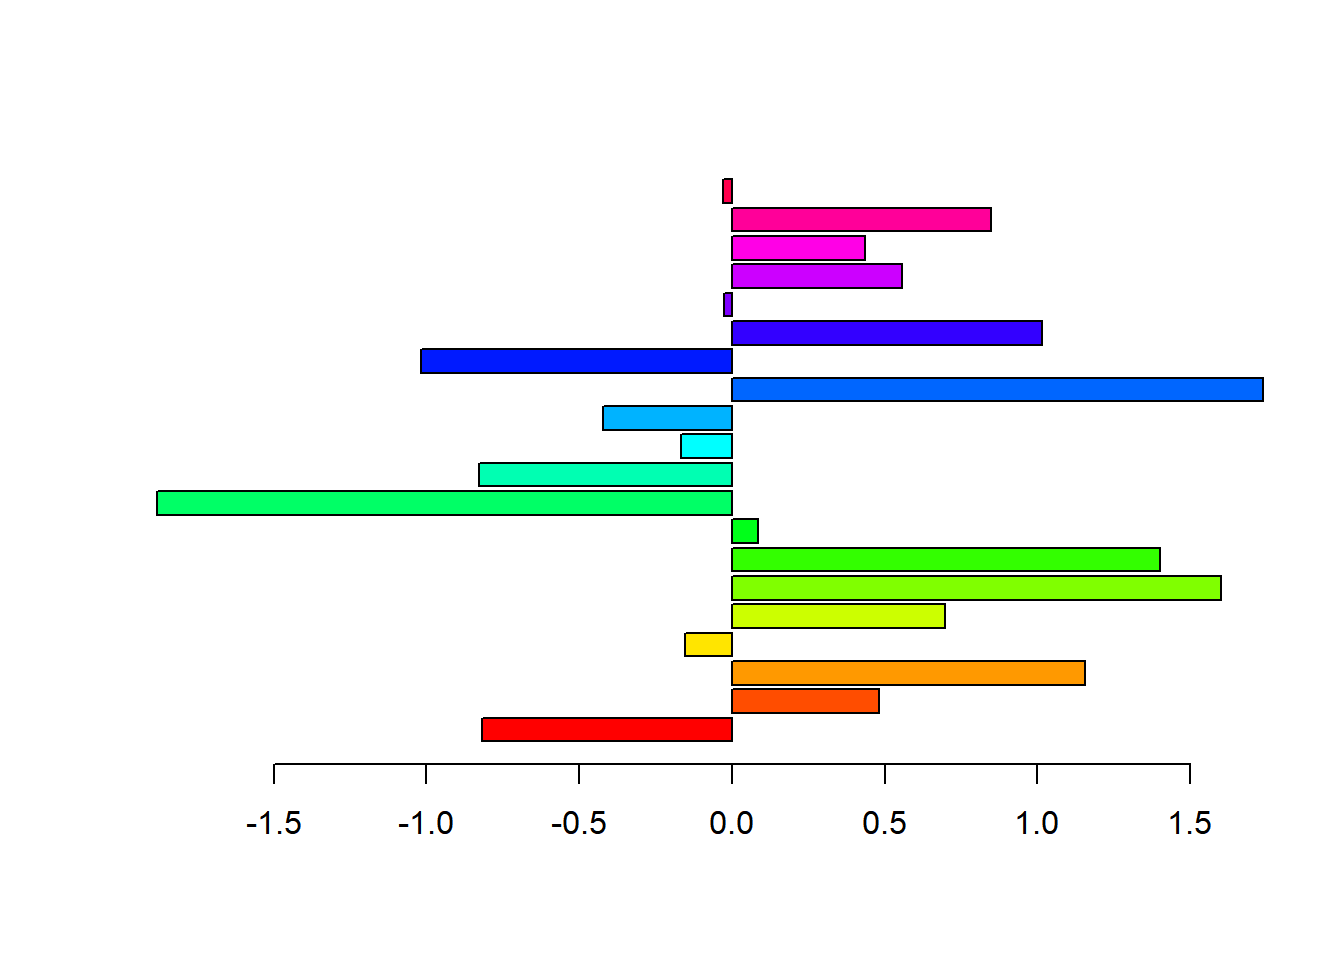
\includegraphics{myRBook_FR_files/figure-latex/unnamed-chunk-237-1.pdf}

Le \texttt{barplot} peut aussi être utilisé pour faire une pyramide des âges (il existe des fonctions pour réaliser des pyramides des âges, ici l'objectif est pédagogique).

\begin{Shaded}
\begin{Highlighting}[]
\NormalTok{gender <-}\StringTok{ }\KeywordTok{data.frame}\NormalTok{(}
  \DataTypeTok{m =} \KeywordTok{cut}\NormalTok{(}\KeywordTok{sample}\NormalTok{(}\DecValTok{1}\OperatorTok{:}\DecValTok{75}\NormalTok{, }\DecValTok{1000}\NormalTok{, }\DataTypeTok{replace =} \OtherTok{TRUE}\NormalTok{), }
    \DataTypeTok{breaks =} \KeywordTok{seq}\NormalTok{(}\DataTypeTok{from =} \DecValTok{0}\NormalTok{, }\DataTypeTok{to =} \DecValTok{80}\NormalTok{, }\DataTypeTok{by =} \DecValTok{10}\NormalTok{)), }
  \DataTypeTok{f =} \KeywordTok{cut}\NormalTok{(}\KeywordTok{sample}\NormalTok{(}\DecValTok{1}\OperatorTok{:}\DecValTok{75}\NormalTok{, }\DecValTok{1000}\NormalTok{, }\DataTypeTok{replace =} \OtherTok{TRUE}\NormalTok{), }
    \DataTypeTok{breaks =} \KeywordTok{seq}\NormalTok{(}\DataTypeTok{from =} \DecValTok{0}\NormalTok{, }\DataTypeTok{to =} \DecValTok{80}\NormalTok{, }\DataTypeTok{by =} \DecValTok{10}\NormalTok{))}
\NormalTok{)}
\NormalTok{op <-}\StringTok{ }\KeywordTok{par}\NormalTok{(}\DataTypeTok{no.readonly =} \OtherTok{TRUE}\NormalTok{)}
\KeywordTok{par}\NormalTok{(}\DataTypeTok{mfrow =} \KeywordTok{c}\NormalTok{(}\DecValTok{1}\NormalTok{, }\DecValTok{2}\NormalTok{), }\DataTypeTok{mar =} \KeywordTok{c}\NormalTok{(}\DecValTok{2}\NormalTok{, }\DecValTok{1}\NormalTok{, }\DecValTok{2}\NormalTok{, }\DecValTok{1}\NormalTok{))}
\KeywordTok{barplot}\NormalTok{(}\OperatorTok{-}\KeywordTok{table}\NormalTok{(gender}\OperatorTok{$}\NormalTok{f), }\DataTypeTok{horiz =} \OtherTok{TRUE}\NormalTok{, }\DataTypeTok{col =} \StringTok{"salmon"}\NormalTok{)}
\KeywordTok{barplot}\NormalTok{(}\KeywordTok{table}\NormalTok{(gender}\OperatorTok{$}\NormalTok{m), }\DataTypeTok{horiz =} \OtherTok{TRUE}\NormalTok{, }\DataTypeTok{col =} \StringTok{"lightblue"}\NormalTok{)}
\end{Highlighting}
\end{Shaded}

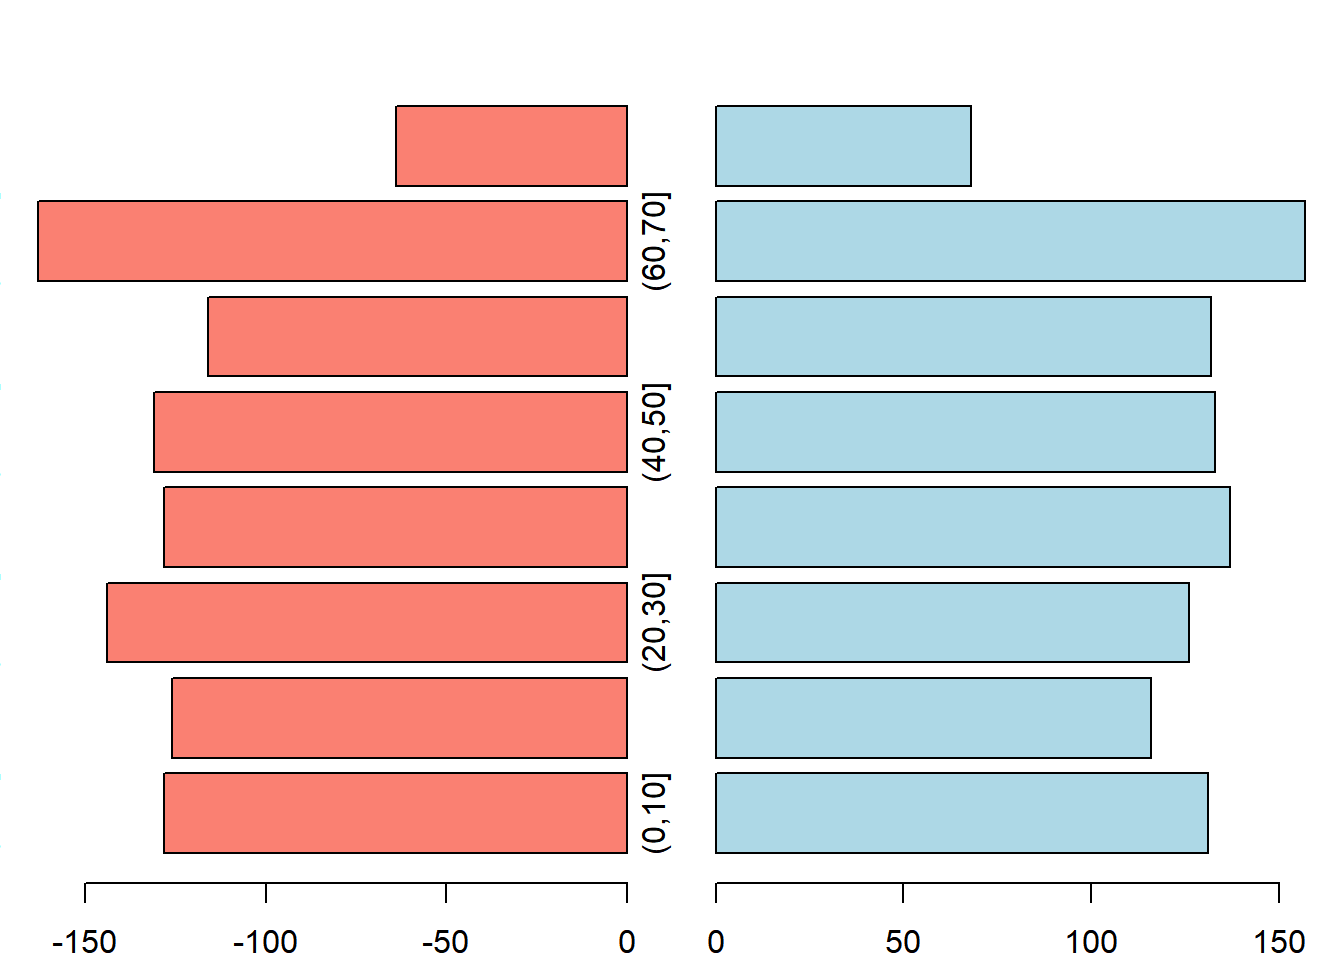
\includegraphics{myRBook_FR_files/figure-latex/unnamed-chunk-238-1.pdf}

\begin{Shaded}
\begin{Highlighting}[]
\KeywordTok{par}\NormalTok{(op)}
\end{Highlighting}
\end{Shaded}

\hypertarget{graph1boxplot}{%
\section{\texorpdfstring{\texttt{boxplot}}{boxplot}}\label{graph1boxplot}}

Les \texttt{boxplot} ou boîtes à moustache sont des graphiques très courant avec R car ils donnent un bon apperçu d'un jeu de données en représentant les valeurs extrèmes (``outliers''), la médiane, les quartiles, les minimums et les maximums.

La fonction \texttt{boxplot()} s'applique à un ou plusieurs \texttt{vector}.

\begin{Shaded}
\begin{Highlighting}[]
\NormalTok{df <-}\StringTok{ }\KeywordTok{data.frame}\NormalTok{(}
  \DataTypeTok{box1 =} \KeywordTok{rnorm}\NormalTok{(}\DecValTok{1000}\NormalTok{), }
  \DataTypeTok{box2 =} \KeywordTok{rgamma}\NormalTok{(}\DecValTok{1000}\NormalTok{, }\DataTypeTok{shape =} \DecValTok{1}\NormalTok{), }
  \DataTypeTok{box3 =} \KeywordTok{sample}\NormalTok{(}\OperatorTok{-}\DecValTok{3}\OperatorTok{:}\DecValTok{3}\NormalTok{, }\DataTypeTok{size =} \DecValTok{1000}\NormalTok{, }\DataTypeTok{replace =} \OtherTok{TRUE}\NormalTok{),}
  \DataTypeTok{box4 =} \KeywordTok{rbeta}\NormalTok{(}\DecValTok{1000}\NormalTok{, }\DataTypeTok{shape1 =} \DecValTok{1}\NormalTok{, }\DataTypeTok{shape2 =} \DecValTok{2}\NormalTok{)}
\NormalTok{)}
\KeywordTok{boxplot}\NormalTok{(df, }\DataTypeTok{col =} \KeywordTok{c}\NormalTok{(}\KeywordTok{rgb}\NormalTok{(}\DecValTok{0}\NormalTok{, }\DecValTok{94}\NormalTok{, }\DecValTok{255}\NormalTok{, }\DataTypeTok{maxColorValue =} \DecValTok{255}\NormalTok{),  }
  \KeywordTok{rgb}\NormalTok{(}\DecValTok{255}\NormalTok{, }\DecValTok{0}\NormalTok{, }\DecValTok{174}\NormalTok{, }\DataTypeTok{maxColorValue =} \DecValTok{255}\NormalTok{),  }
  \KeywordTok{rgb}\NormalTok{(}\DecValTok{255}\NormalTok{, }\DecValTok{136}\NormalTok{, }\DecValTok{0}\NormalTok{, }\DataTypeTok{maxColorValue =} \DecValTok{255}\NormalTok{),  }
  \KeywordTok{rgb}\NormalTok{(}\DecValTok{119}\NormalTok{, }\DecValTok{255}\NormalTok{, }\DecValTok{0}\NormalTok{, }\DataTypeTok{maxColorValue =} \DecValTok{255}\NormalTok{)))}
\end{Highlighting}
\end{Shaded}

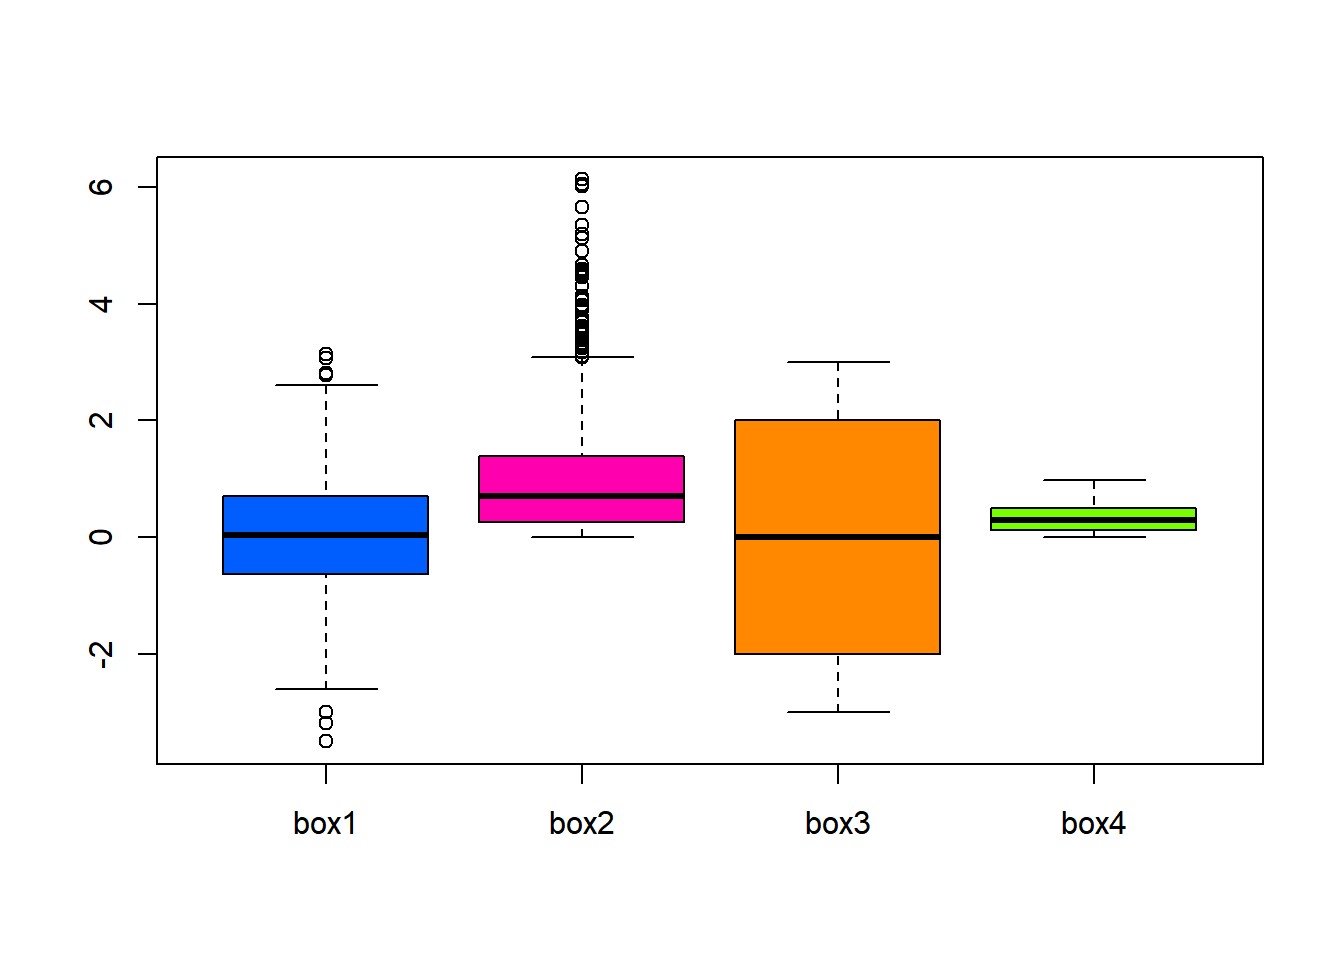
\includegraphics{myRBook_FR_files/figure-latex/unnamed-chunk-239-1.pdf}

Si une variable est de type \texttt{factor}, la fonction \texttt{boxplot()} permet facilement de représenter chaque catégorie. Cela fonctionne aussi avec les variables numériques mais il faut veiller à ne pas avoir trop de valeurs différentes pour que le graphique reste lisible.

\begin{Shaded}
\begin{Highlighting}[]
\NormalTok{df}\OperatorTok{$}\NormalTok{cat <-}\StringTok{ }\KeywordTok{sample}\NormalTok{(}\KeywordTok{c}\NormalTok{(}\StringTok{"w"}\NormalTok{, }\StringTok{"x"}\NormalTok{, }\StringTok{"y"}\NormalTok{, }\StringTok{"z"}\NormalTok{), }\DataTypeTok{size =} \DecValTok{1000}\NormalTok{, }\DataTypeTok{replace =} \OtherTok{TRUE}\NormalTok{)}
\KeywordTok{boxplot}\NormalTok{(df}\OperatorTok{$}\NormalTok{box3 }\OperatorTok{~}\StringTok{ }\NormalTok{df}\OperatorTok{$}\NormalTok{cat, }\DataTypeTok{col =} \KeywordTok{c}\NormalTok{(}\KeywordTok{rgb}\NormalTok{(}\DecValTok{0}\NormalTok{, }\DecValTok{94}\NormalTok{, }\DecValTok{255}\NormalTok{, }\DataTypeTok{maxColorValue =} \DecValTok{255}\NormalTok{),  }
  \KeywordTok{rgb}\NormalTok{(}\DecValTok{255}\NormalTok{, }\DecValTok{0}\NormalTok{, }\DecValTok{174}\NormalTok{, }\DataTypeTok{maxColorValue =} \DecValTok{255}\NormalTok{),  }
  \KeywordTok{rgb}\NormalTok{(}\DecValTok{255}\NormalTok{, }\DecValTok{136}\NormalTok{, }\DecValTok{0}\NormalTok{, }\DataTypeTok{maxColorValue =} \DecValTok{255}\NormalTok{),  }
  \KeywordTok{rgb}\NormalTok{(}\DecValTok{119}\NormalTok{, }\DecValTok{255}\NormalTok{, }\DecValTok{0}\NormalTok{, }\DataTypeTok{maxColorValue =} \DecValTok{255}\NormalTok{)), }\DataTypeTok{ylab =} \StringTok{"Box3"}\NormalTok{)}
\end{Highlighting}
\end{Shaded}

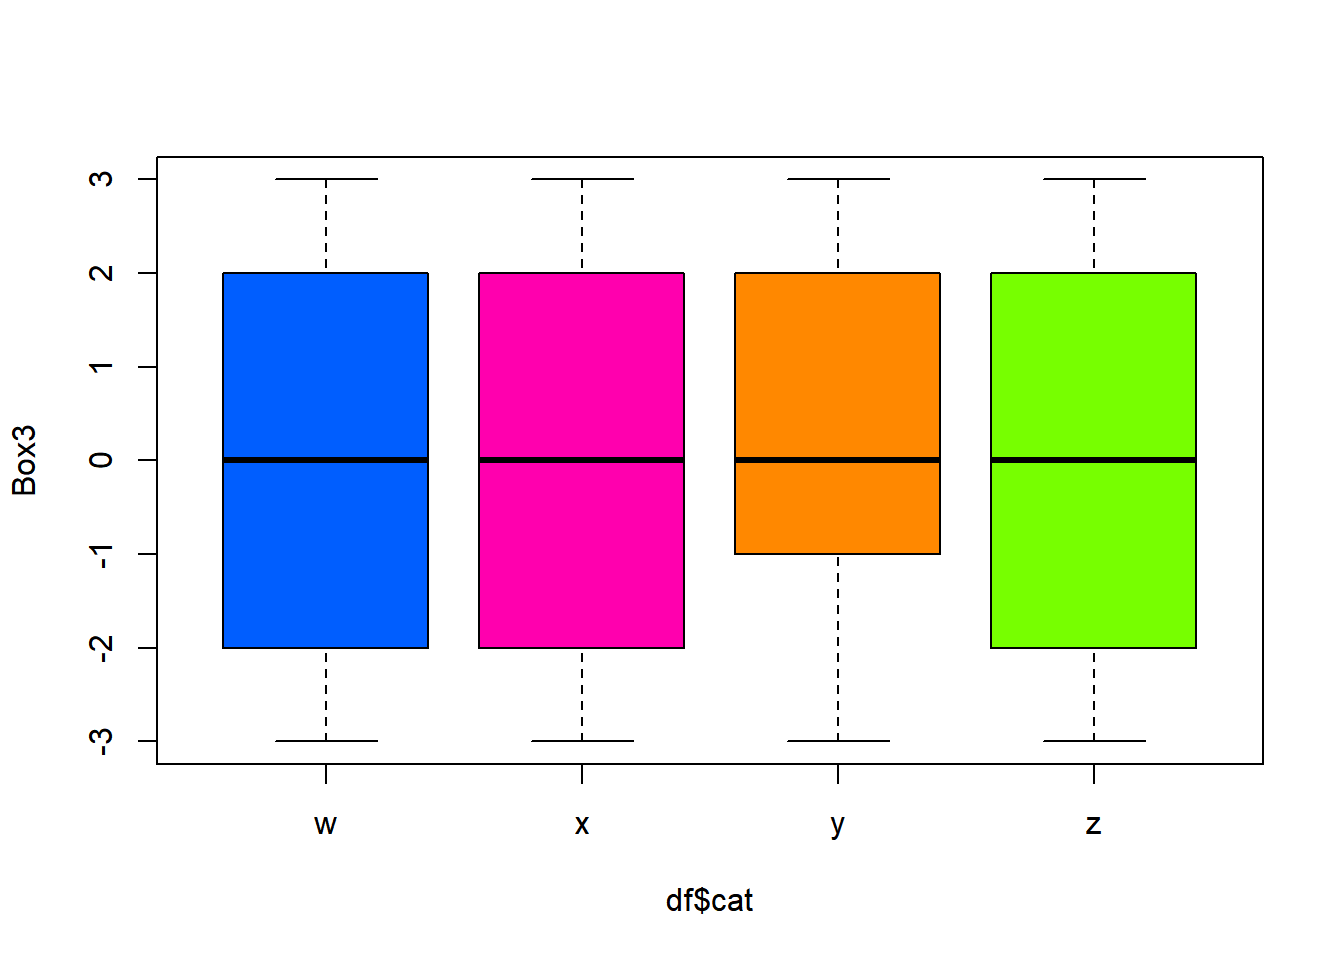
\includegraphics{myRBook_FR_files/figure-latex/unnamed-chunk-240-1.pdf}

\begin{Shaded}
\begin{Highlighting}[]
\NormalTok{df}\OperatorTok{$}\NormalTok{cat2 <-}\StringTok{ }\KeywordTok{sample}\NormalTok{(}\DecValTok{1}\OperatorTok{:}\DecValTok{3}\NormalTok{, }\DataTypeTok{size =} \DecValTok{1000}\NormalTok{, }\DataTypeTok{replace =} \OtherTok{TRUE}\NormalTok{)}
\KeywordTok{boxplot}\NormalTok{(df}\OperatorTok{$}\NormalTok{box4 }\OperatorTok{~}\StringTok{ }\NormalTok{df}\OperatorTok{$}\NormalTok{cat}\OperatorTok{*}\NormalTok{df}\OperatorTok{$}\NormalTok{cat2, }\DataTypeTok{col =} \KeywordTok{c}\NormalTok{(}
  \KeywordTok{rgb}\NormalTok{(}\DecValTok{0}\NormalTok{, }\DecValTok{94}\NormalTok{, }\DecValTok{255}\NormalTok{, }\DataTypeTok{maxColorValue =} \DecValTok{255}\NormalTok{),  }
  \KeywordTok{rgb}\NormalTok{(}\DecValTok{255}\NormalTok{, }\DecValTok{0}\NormalTok{, }\DecValTok{174}\NormalTok{, }\DataTypeTok{maxColorValue =} \DecValTok{255}\NormalTok{),  }
  \KeywordTok{rgb}\NormalTok{(}\DecValTok{255}\NormalTok{, }\DecValTok{136}\NormalTok{, }\DecValTok{0}\NormalTok{, }\DataTypeTok{maxColorValue =} \DecValTok{255}\NormalTok{),  }
  \KeywordTok{rgb}\NormalTok{(}\DecValTok{119}\NormalTok{, }\DecValTok{255}\NormalTok{, }\DecValTok{0}\NormalTok{, }\DataTypeTok{maxColorValue =} \DecValTok{255}\NormalTok{)), }\DataTypeTok{ylab =} \StringTok{"Box4"}\NormalTok{)}
\end{Highlighting}
\end{Shaded}

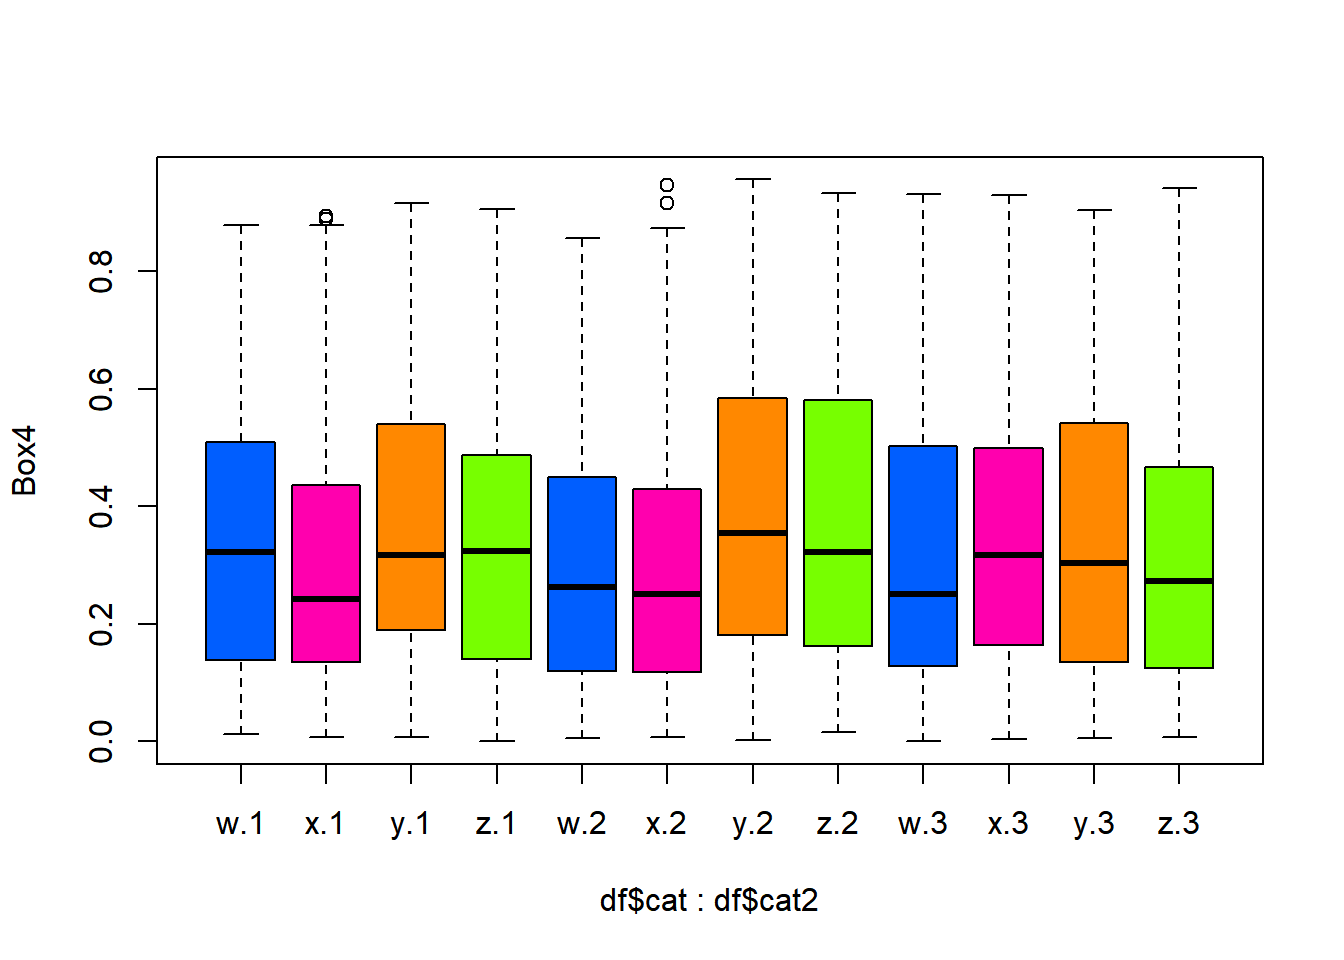
\includegraphics{myRBook_FR_files/figure-latex/unnamed-chunk-240-2.pdf}

Le \texttt{boxplot} peut être représenté horizontalement ou verticalement.

\begin{Shaded}
\begin{Highlighting}[]
\NormalTok{df}\OperatorTok{$}\NormalTok{cat <-}\StringTok{ }\KeywordTok{sample}\NormalTok{(}\KeywordTok{c}\NormalTok{(}\StringTok{"w"}\NormalTok{, }\StringTok{"x"}\NormalTok{, }\StringTok{"y"}\NormalTok{, }\StringTok{"z"}\NormalTok{), }\DataTypeTok{size =} \DecValTok{1000}\NormalTok{, }\DataTypeTok{replace =} \OtherTok{TRUE}\NormalTok{)}
\KeywordTok{boxplot}\NormalTok{(df}\OperatorTok{$}\NormalTok{box2 }\OperatorTok{~}\StringTok{ }\NormalTok{df}\OperatorTok{$}\NormalTok{cat, }\DataTypeTok{horizontal =} \OtherTok{TRUE}\NormalTok{, }
  \DataTypeTok{col =} \KeywordTok{c}\NormalTok{(}\KeywordTok{rgb}\NormalTok{(}\DecValTok{255}\NormalTok{, }\DecValTok{110}\NormalTok{, }\DecValTok{0}\NormalTok{, }\DataTypeTok{maxColorValue =} \DecValTok{255}\NormalTok{),  }
  \KeywordTok{rgb}\NormalTok{(}\DecValTok{230}\NormalTok{, }\DecValTok{255}\NormalTok{, }\DecValTok{0}\NormalTok{, }\DataTypeTok{maxColorValue =} \DecValTok{255}\NormalTok{),  }
  \KeywordTok{rgb}\NormalTok{(}\DecValTok{0}\NormalTok{, }\DecValTok{178}\NormalTok{, }\DecValTok{255}\NormalTok{, }\DataTypeTok{maxColorValue =} \DecValTok{255}\NormalTok{),  }
  \KeywordTok{rgb}\NormalTok{(}\DecValTok{166}\NormalTok{, }\DecValTok{0}\NormalTok{, }\DecValTok{255}\NormalTok{, }\DataTypeTok{maxColorValue =} \DecValTok{255}\NormalTok{)), }\DataTypeTok{xlab =} \StringTok{"Box2"}\NormalTok{)}
\end{Highlighting}
\end{Shaded}

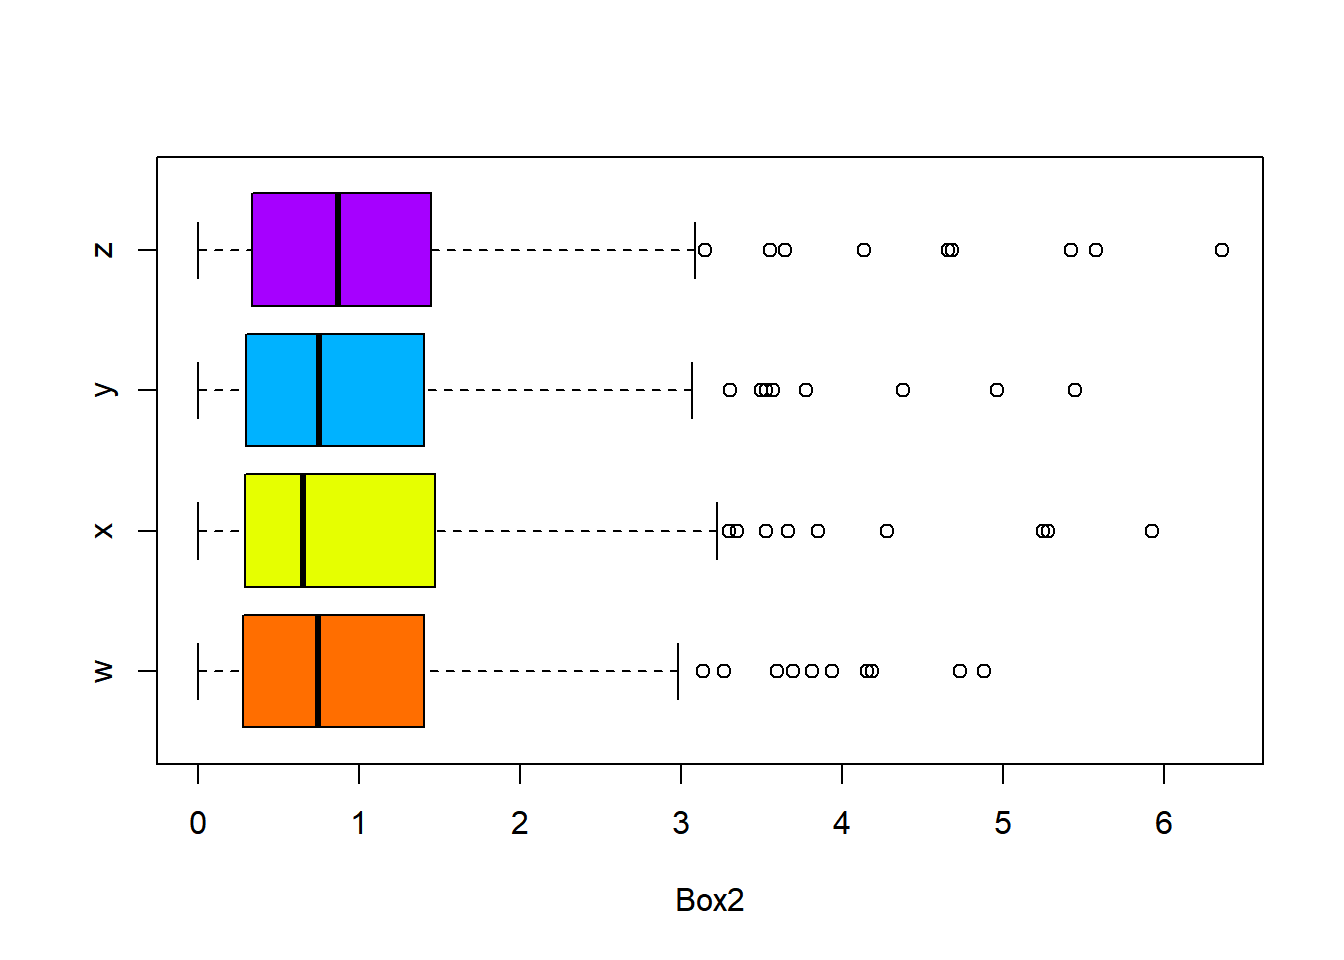
\includegraphics{myRBook_FR_files/figure-latex/unnamed-chunk-241-1.pdf}

\hypertarget{autres-graphiques}{%
\section{Autres graphiques}\label{autres-graphiques}}

Il existe de nombreux autres graphiques mais ceux que nous venons de voir constituent la base. Pour plus d'information et d'idées pour représenter vos données nous pouvons consulter le très beau site \url{https://www.data-to-viz.com/} ou encore la gallerie de graphiques R \url{https://www.r-graph-gallery.com/} (en anglais ; la plupart des graphiques sont réalisés avec le package ggplot2 que nous verrons plus tard). Pour plus d'idées vous pouvez aussi utiliser la demonstration du package \texttt{graphics} en utilisant la commande \texttt{demo("graphics")} (la touche ``Entrée'' permet d'afficher les graphiques).

\hypertarget{conclusion-8}{%
\section{Conclusion}\label{conclusion-8}}

Félicitations, nous sommes arrivés à la fin de ce chapitre sur les graphiques simples ! Nous savons désormais réaliser les principaux graphiques \texttt{plot()}, \texttt{hist()}, \texttt{barplot()}, et \texttt{boxplot()}. Tout au long de ce chapitre nous avons utilisé différentes couleurs et différentes façons de représenter les couleurs : il est temps de formaliser l'utilisation et la gestion des couleurs. C'est le sujet du prochain chapitre !

\hypertarget{graph2}{%
\chapter{La gestion des couleurs}\label{graph2}}

Nous avons vu différentes manières d'utiliser les couleurs : avec leur nom (e.g., \texttt{"salmon"}), avec un numéro de 1 à 8, avec la fonction \texttt{rgb()} (pour ``red'', ``green'', ``blue''), et avec la fonction \texttt{colors()}. Il en existe d'autres mais celles-ci sont les principales.

L'utilisation des numéros de 1 à 8 correspond au noir, rouge, vert, bleu, cyan, magenta, jaune et gris. Cette utilisation est pratique pour visualiser rapidement nos résultats mais donne globalement des graphiques visuellement moyens. Ces couleurs sont plutôt à éviter pour communiquer nos graphiques.

\begin{Shaded}
\begin{Highlighting}[]
\KeywordTok{barplot}\NormalTok{(}\KeywordTok{sample}\NormalTok{(}\DecValTok{10}\OperatorTok{:}\DecValTok{15}\NormalTok{, }\DecValTok{8}\NormalTok{, }\DataTypeTok{replace =} \OtherTok{TRUE}\NormalTok{), }\DataTypeTok{col =} \DecValTok{1}\OperatorTok{:}\DecValTok{8}\NormalTok{, }\DataTypeTok{names.arg =} \DecValTok{1}\OperatorTok{:}\DecValTok{8}\NormalTok{)}
\end{Highlighting}
\end{Shaded}

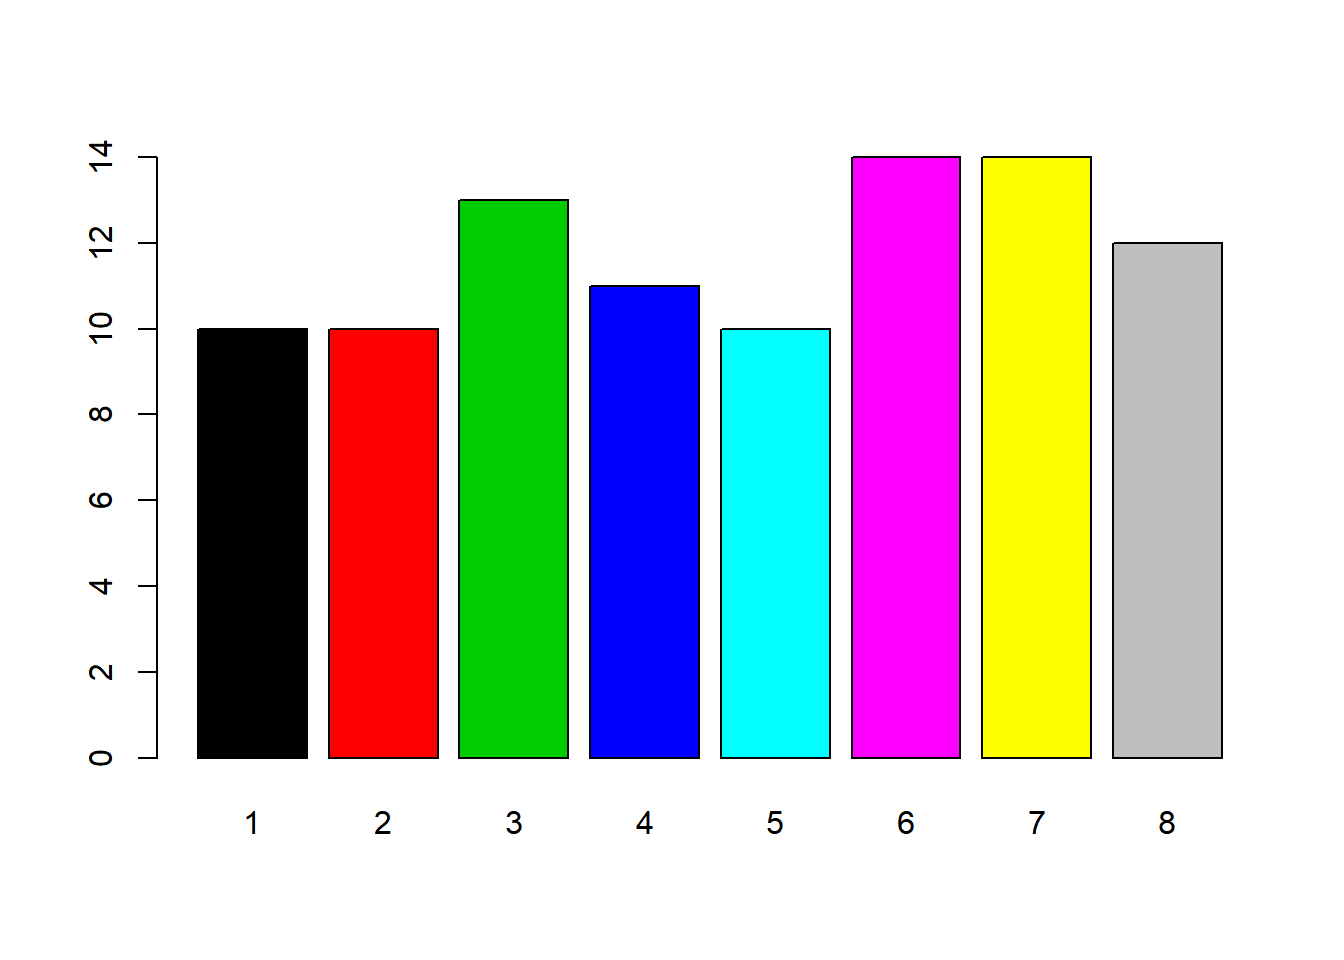
\includegraphics{myRBook_FR_files/figure-latex/unnamed-chunk-242-1.pdf}

\hypertarget{colors}{%
\section{\texorpdfstring{\texttt{colors()}}{colors()}}\label{colors}}

Pour choisir des couleurs plus agréables et mettant plus en avant nos résultats, une option consiste à les choisir dans la liste des couleurs pré-enregistrées dans R. Nous pouvons accéder à la liste des couleurs avec la fonction \texttt{colors()}

\begin{Shaded}
\begin{Highlighting}[]
\KeywordTok{head}\NormalTok{(}\KeywordTok{colors}\NormalTok{(), }\DataTypeTok{n =} \DecValTok{20}\NormalTok{)}
\end{Highlighting}
\end{Shaded}

\begin{verbatim}
##  [1] "white"         "aliceblue"     "antiquewhite"  "antiquewhite1"
##  [5] "antiquewhite2" "antiquewhite3" "antiquewhite4" "aquamarine"   
##  [9] "aquamarine1"   "aquamarine2"   "aquamarine3"   "aquamarine4"  
## [13] "azure"         "azure1"        "azure2"        "azure3"       
## [17] "azure4"        "beige"         "bisque"        "bisque1"
\end{verbatim}

Nous pouvons utiliser ces couleurs avec leur nom (e.g., ``white'', ``azure3''), ou alors avec leur numéro (e.g., ``white'' = \texttt{colors(){[}1{]}}, ``azure3'' = \texttt{colors(){[}16{]}}).

\begin{Shaded}
\begin{Highlighting}[]
\CommentTok{# adapted from http://www.r-graph-gallery.com/42-colors-names/}
\NormalTok{op <-}\StringTok{ }\KeywordTok{par}\NormalTok{(}\DataTypeTok{no.readonly =} \OtherTok{TRUE}\NormalTok{)}
\KeywordTok{par}\NormalTok{(}\DataTypeTok{mar =} \KeywordTok{c}\NormalTok{(}\DecValTok{0}\NormalTok{, }\DecValTok{0}\NormalTok{, }\DecValTok{0}\NormalTok{, }\DecValTok{0}\NormalTok{))}
\KeywordTok{plot}\NormalTok{(}\DecValTok{0}\NormalTok{, }\DataTypeTok{type =} \StringTok{"n"}\NormalTok{, }\DataTypeTok{xlim =} \KeywordTok{c}\NormalTok{(}\DecValTok{0}\NormalTok{, }\DecValTok{1}\NormalTok{), }\DataTypeTok{ylim =} \KeywordTok{c}\NormalTok{(}\DecValTok{0}\NormalTok{, }\DecValTok{1}\NormalTok{), }
  \DataTypeTok{axes =} \OtherTok{FALSE}\NormalTok{, }\DataTypeTok{xlab =} \StringTok{""}\NormalTok{, }\DataTypeTok{ylab =} \StringTok{""}\NormalTok{)}
\NormalTok{numRow <-}\StringTok{ }\DecValTok{26}
\NormalTok{numCol <-}\StringTok{ }\DecValTok{26}
\KeywordTok{rect}\NormalTok{(}
  \DataTypeTok{xleft =} \KeywordTok{rep}\NormalTok{((}\DecValTok{0}\OperatorTok{:}\NormalTok{(numCol }\OperatorTok{-}\StringTok{ }\DecValTok{1}\NormalTok{)}\OperatorTok{/}\NormalTok{numCol), numRow),  }
  \DataTypeTok{ybottom =} \KeywordTok{sort}\NormalTok{(}\KeywordTok{rep}\NormalTok{((}\DecValTok{0}\OperatorTok{:}\NormalTok{(numRow }\OperatorTok{-}\StringTok{ }\DecValTok{1}\NormalTok{)}\OperatorTok{/}\NormalTok{numRow),numCol), }\DataTypeTok{decreasing =} \OtherTok{TRUE}\NormalTok{),}
  \DataTypeTok{xright =} \KeywordTok{rep}\NormalTok{((}\DecValTok{1}\OperatorTok{:}\NormalTok{numCol}\OperatorTok{/}\NormalTok{numCol), numRow),}
  \DataTypeTok{ytop =} \KeywordTok{sort}\NormalTok{(}\KeywordTok{rep}\NormalTok{((}\DecValTok{1}\OperatorTok{:}\NormalTok{numRow}\OperatorTok{/}\NormalTok{numRow), numCol), }\DataTypeTok{decreasing =} \OtherTok{TRUE}\NormalTok{),}
  \DataTypeTok{border =} \KeywordTok{grey}\NormalTok{(}\FloatTok{0.5}\NormalTok{), }
  \DataTypeTok{col =} \KeywordTok{colors}\NormalTok{()[}\KeywordTok{seq}\NormalTok{(}\DecValTok{1}\NormalTok{, numRow}\OperatorTok{*}\NormalTok{numCol)])}
\NormalTok{myLabels <-}\StringTok{ }\KeywordTok{c}\NormalTok{(}\KeywordTok{as.character}\NormalTok{(}\DecValTok{1}\OperatorTok{:}\DecValTok{657}\NormalTok{), }\KeywordTok{rep}\NormalTok{(}\StringTok{""}\NormalTok{, numRow}\OperatorTok{*}\NormalTok{numCol }\OperatorTok{-}\StringTok{ }\DecValTok{657}\NormalTok{))}
\KeywordTok{text}\NormalTok{(}
  \DataTypeTok{x =} \KeywordTok{rep}\NormalTok{((}\DecValTok{0}\OperatorTok{:}\NormalTok{(numCol }\OperatorTok{-}\StringTok{ }\DecValTok{1}\NormalTok{)}\OperatorTok{/}\NormalTok{numCol), numRow) }\OperatorTok{+}\StringTok{ }\FloatTok{0.02}\NormalTok{,}
  \DataTypeTok{y =} \KeywordTok{sort}\NormalTok{(}\KeywordTok{rep}\NormalTok{((}\DecValTok{0}\OperatorTok{:}\NormalTok{(numRow }\OperatorTok{-}\StringTok{ }\DecValTok{1}\NormalTok{)}\OperatorTok{/}\NormalTok{numRow), numCol), }\DataTypeTok{decreasing =} \OtherTok{TRUE}\NormalTok{) }\OperatorTok{+}\StringTok{ }\FloatTok{0.02}\NormalTok{,}
  \DataTypeTok{labels =}\NormalTok{ myLabels, }
  \DataTypeTok{cex =} \FloatTok{0.6}\NormalTok{)}
\end{Highlighting}
\end{Shaded}

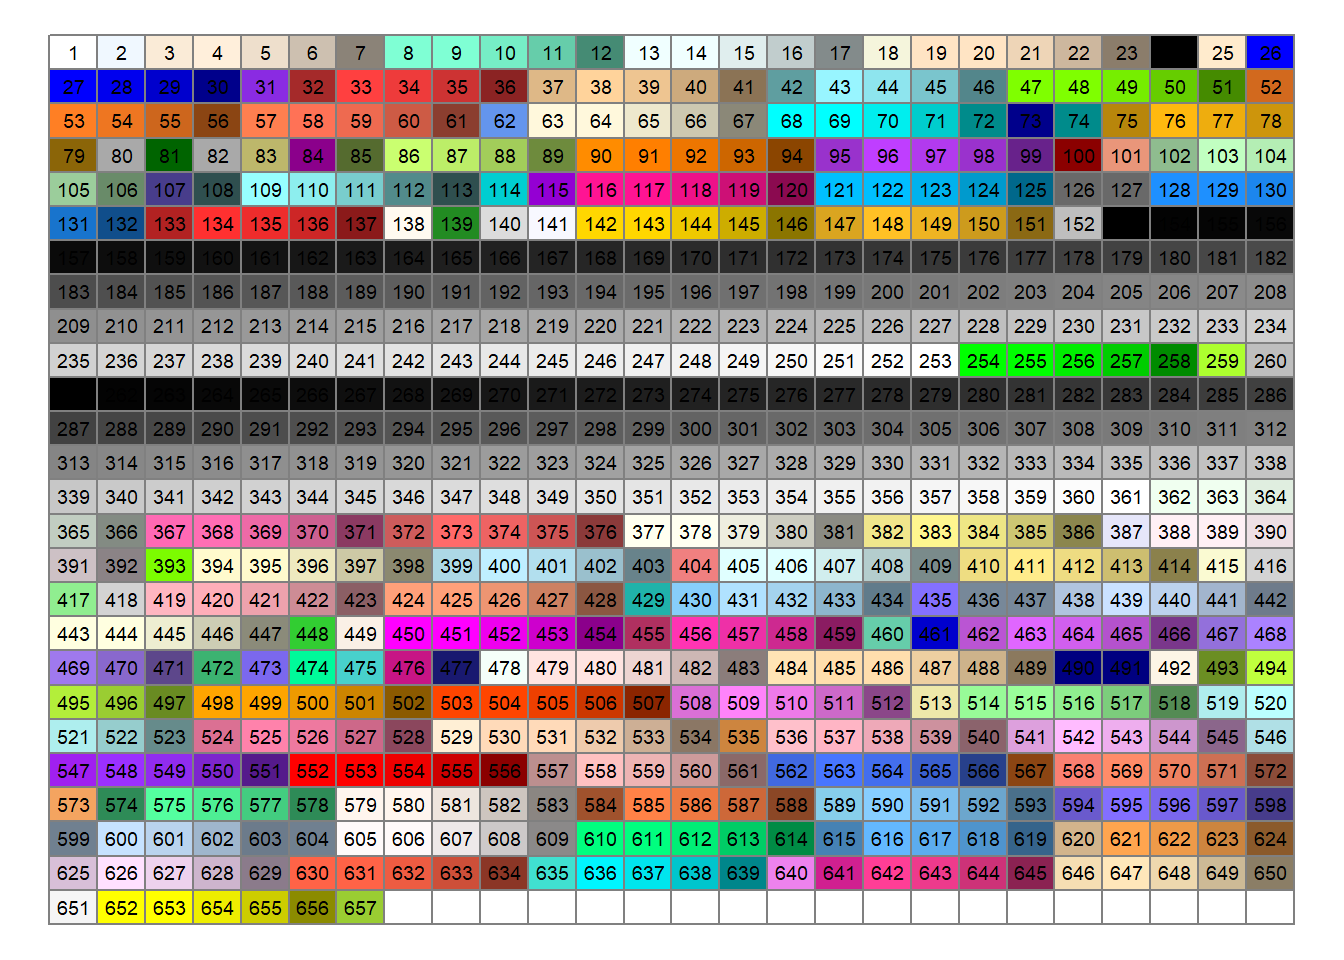
\includegraphics{myRBook_FR_files/figure-latex/unnamed-chunk-244-1.pdf}

\begin{Shaded}
\begin{Highlighting}[]
\KeywordTok{par}\NormalTok{(op)}
\end{Highlighting}
\end{Shaded}

\hypertarget{rgb}{%
\section{\texorpdfstring{\texttt{rgb()}}{rgb()}}\label{rgb}}

Une autre option consiste à construire ses propres couleurs ave la fonction \texttt{rgb()} qui prend comme argument la quantité de rouge, de de vert, et de bleu. Par défaut ces valeurs sont comprises entre 0 et 1. Ce réglage par défaut peut être modifié avec l'arguement \texttt{maxColorValue} pour par exemple avoir des valeurs entre 0 et 255 (\texttt{maxColorValue\ =\ 255} ; norme pour la représentation des couleurs RGB).

Nous allons reprendre notre fonction permettant de représenter la distribution de points dans un nuage de points au moyen de \texttt{barplot} avec cette fois trois couleurs de points (rouge, vert, bleu), et des \texttt{barplot} dont la couleur correspondra à la quantité de chaque couleur avec la fonction \texttt{rgb()}.

\begin{Shaded}
\begin{Highlighting}[]
\NormalTok{graphBarplotCol <-}\StringTok{ }\ControlFlowTok{function}\NormalTok{(n)\{}
\NormalTok{  myX <-}\StringTok{ }\KeywordTok{rnorm}\NormalTok{(n)}
\NormalTok{  myY <-}\StringTok{ }\KeywordTok{rnorm}\NormalTok{(n)}
\NormalTok{  myCol <-}\StringTok{ }\KeywordTok{c}\NormalTok{(}\DecValTok{2}\NormalTok{, }\DecValTok{3}\NormalTok{, }\DecValTok{4}\NormalTok{, }\KeywordTok{sample}\NormalTok{(}\DecValTok{2}\OperatorTok{:}\DecValTok{4}\NormalTok{, }\DataTypeTok{size =}\NormalTok{ (n }\OperatorTok{-}\StringTok{ }\DecValTok{3}\NormalTok{), }\DataTypeTok{replace =} \OtherTok{TRUE}\NormalTok{))}
\NormalTok{  myYCut <-}\StringTok{ }\KeywordTok{cut}\NormalTok{(myY, }\DataTypeTok{breaks =} \DecValTok{-4}\OperatorTok{:}\DecValTok{4}\NormalTok{)}
\NormalTok{  myXCut <-}\StringTok{ }\KeywordTok{cut}\NormalTok{(myX, }\DataTypeTok{breaks =} \DecValTok{-4}\OperatorTok{:}\DecValTok{4}\NormalTok{)}
\NormalTok{  myYCutCol <-}\StringTok{ }\KeywordTok{table}\NormalTok{(myCol, myYCut)}
\NormalTok{  myXCutCol <-}\StringTok{ }\KeywordTok{table}\NormalTok{(myCol, myXCut)}
\NormalTok{  rColX <-}\StringTok{ }\NormalTok{myXCutCol[}\DecValTok{1}\NormalTok{,] }\OperatorTok{/}\StringTok{ }\NormalTok{(myXCutCol[}\DecValTok{1}\NormalTok{,] }\OperatorTok{+}\StringTok{ }\NormalTok{myXCutCol[}\DecValTok{2}\NormalTok{,] }\OperatorTok{+}\StringTok{ }
\StringTok{    }\NormalTok{myXCutCol[}\DecValTok{3}\NormalTok{,])}
\NormalTok{  gColX <-}\StringTok{ }\NormalTok{myXCutCol[}\DecValTok{2}\NormalTok{,] }\OperatorTok{/}\StringTok{ }\NormalTok{(myXCutCol[}\DecValTok{1}\NormalTok{,] }\OperatorTok{+}\StringTok{ }\NormalTok{myXCutCol[}\DecValTok{2}\NormalTok{,] }\OperatorTok{+}\StringTok{ }
\StringTok{    }\NormalTok{myXCutCol[}\DecValTok{3}\NormalTok{,])}
\NormalTok{  bColX <-}\StringTok{ }\NormalTok{myXCutCol[}\DecValTok{3}\NormalTok{,] }\OperatorTok{/}\StringTok{ }\NormalTok{(myXCutCol[}\DecValTok{1}\NormalTok{,] }\OperatorTok{+}\StringTok{ }\NormalTok{myXCutCol[}\DecValTok{2}\NormalTok{,] }\OperatorTok{+}\StringTok{ }
\StringTok{    }\NormalTok{myXCutCol[}\DecValTok{3}\NormalTok{,])}
\NormalTok{  rColX[}\KeywordTok{is.na}\NormalTok{(rColX)] <-}\StringTok{ }\DecValTok{0}
\NormalTok{  gColX[}\KeywordTok{is.na}\NormalTok{(gColX)] <-}\StringTok{ }\DecValTok{0}
\NormalTok{  bColX[}\KeywordTok{is.na}\NormalTok{(bColX)] <-}\StringTok{ }\DecValTok{0}
\NormalTok{  rColY <-}\StringTok{ }\NormalTok{myYCutCol[}\DecValTok{1}\NormalTok{,] }\OperatorTok{/}\StringTok{ }\NormalTok{(myYCutCol[}\DecValTok{1}\NormalTok{,] }\OperatorTok{+}\StringTok{ }\NormalTok{myYCutCol[}\DecValTok{2}\NormalTok{,] }\OperatorTok{+}\StringTok{ }
\StringTok{    }\NormalTok{myYCutCol[}\DecValTok{3}\NormalTok{,])}
\NormalTok{  gColY <-}\StringTok{ }\NormalTok{myYCutCol[}\DecValTok{2}\NormalTok{,] }\OperatorTok{/}\StringTok{ }\NormalTok{(myYCutCol[}\DecValTok{1}\NormalTok{,] }\OperatorTok{+}\StringTok{ }\NormalTok{myYCutCol[}\DecValTok{2}\NormalTok{,] }\OperatorTok{+}\StringTok{ }
\StringTok{    }\NormalTok{myYCutCol[}\DecValTok{3}\NormalTok{,])}
\NormalTok{  bColY <-}\StringTok{ }\NormalTok{myYCutCol[}\DecValTok{3}\NormalTok{,] }\OperatorTok{/}\StringTok{ }\NormalTok{(myYCutCol[}\DecValTok{1}\NormalTok{,] }\OperatorTok{+}\StringTok{ }\NormalTok{myYCutCol[}\DecValTok{2}\NormalTok{,] }\OperatorTok{+}\StringTok{ }
\StringTok{    }\NormalTok{myYCutCol[}\DecValTok{3}\NormalTok{,])}
\NormalTok{  rColY[}\KeywordTok{is.na}\NormalTok{(rColY)] <-}\StringTok{ }\DecValTok{0}
\NormalTok{  gColY[}\KeywordTok{is.na}\NormalTok{(gColY)] <-}\StringTok{ }\DecValTok{0}
\NormalTok{  bColY[}\KeywordTok{is.na}\NormalTok{(bColY)] <-}\StringTok{ }\DecValTok{0}
\NormalTok{  op <-}\StringTok{ }\KeywordTok{par}\NormalTok{(}\DataTypeTok{no.readonly =} \OtherTok{TRUE}\NormalTok{)}
  \KeywordTok{par}\NormalTok{(}\DataTypeTok{mar =} \KeywordTok{c}\NormalTok{(}\DecValTok{2}\NormalTok{, }\DecValTok{3}\NormalTok{, }\DecValTok{1}\NormalTok{, }\DecValTok{1}\NormalTok{))}
  \KeywordTok{layout}\NormalTok{(}\KeywordTok{matrix}\NormalTok{(}\KeywordTok{c}\NormalTok{(}\DecValTok{1}\NormalTok{, }\DecValTok{1}\NormalTok{, }\DecValTok{0}\NormalTok{, }
                  \DecValTok{2}\NormalTok{, }\DecValTok{2}\NormalTok{, }\DecValTok{3}\NormalTok{, }
                  \DecValTok{2}\NormalTok{, }\DecValTok{2}\NormalTok{, }\DecValTok{3}\NormalTok{), }\DataTypeTok{ncol =} \DecValTok{3}\NormalTok{, }\DataTypeTok{byrow =} \OtherTok{TRUE}\NormalTok{))}
  \KeywordTok{barplot}\NormalTok{(}\KeywordTok{table}\NormalTok{(myXCut), }\DataTypeTok{las =} \DecValTok{1}\NormalTok{, }\DataTypeTok{col =} \KeywordTok{rgb}\NormalTok{(rColX, gColX, bColX))}
  \KeywordTok{plot}\NormalTok{(}\DataTypeTok{x =}\NormalTok{ myX, }\DataTypeTok{y =}\NormalTok{ myY, }\DataTypeTok{col =}\NormalTok{ myCol, }\DataTypeTok{pch =} \DecValTok{16}\NormalTok{, }
    \DataTypeTok{xlim =} \KeywordTok{c}\NormalTok{(}\OperatorTok{-}\DecValTok{4}\NormalTok{, }\DecValTok{4}\NormalTok{), }\DataTypeTok{ylim =} \KeywordTok{c}\NormalTok{(}\OperatorTok{-}\DecValTok{4}\NormalTok{, }\DecValTok{4}\NormalTok{), }\DataTypeTok{cex =} \FloatTok{1.5}\NormalTok{, }
    \DataTypeTok{panel.first =} \KeywordTok{grid}\NormalTok{())}
  \KeywordTok{barplot}\NormalTok{(}\KeywordTok{table}\NormalTok{(myYCut), }\DataTypeTok{las =} \DecValTok{1}\NormalTok{, }\DataTypeTok{horiz =} \OtherTok{TRUE}\NormalTok{, }
    \DataTypeTok{col =} \KeywordTok{rgb}\NormalTok{(rColY, gColY, bColY))}
  \KeywordTok{par}\NormalTok{(op)}
\NormalTok{\}}
\KeywordTok{graphBarplotCol}\NormalTok{(}\DataTypeTok{n =} \DecValTok{50}\NormalTok{)}
\end{Highlighting}
\end{Shaded}

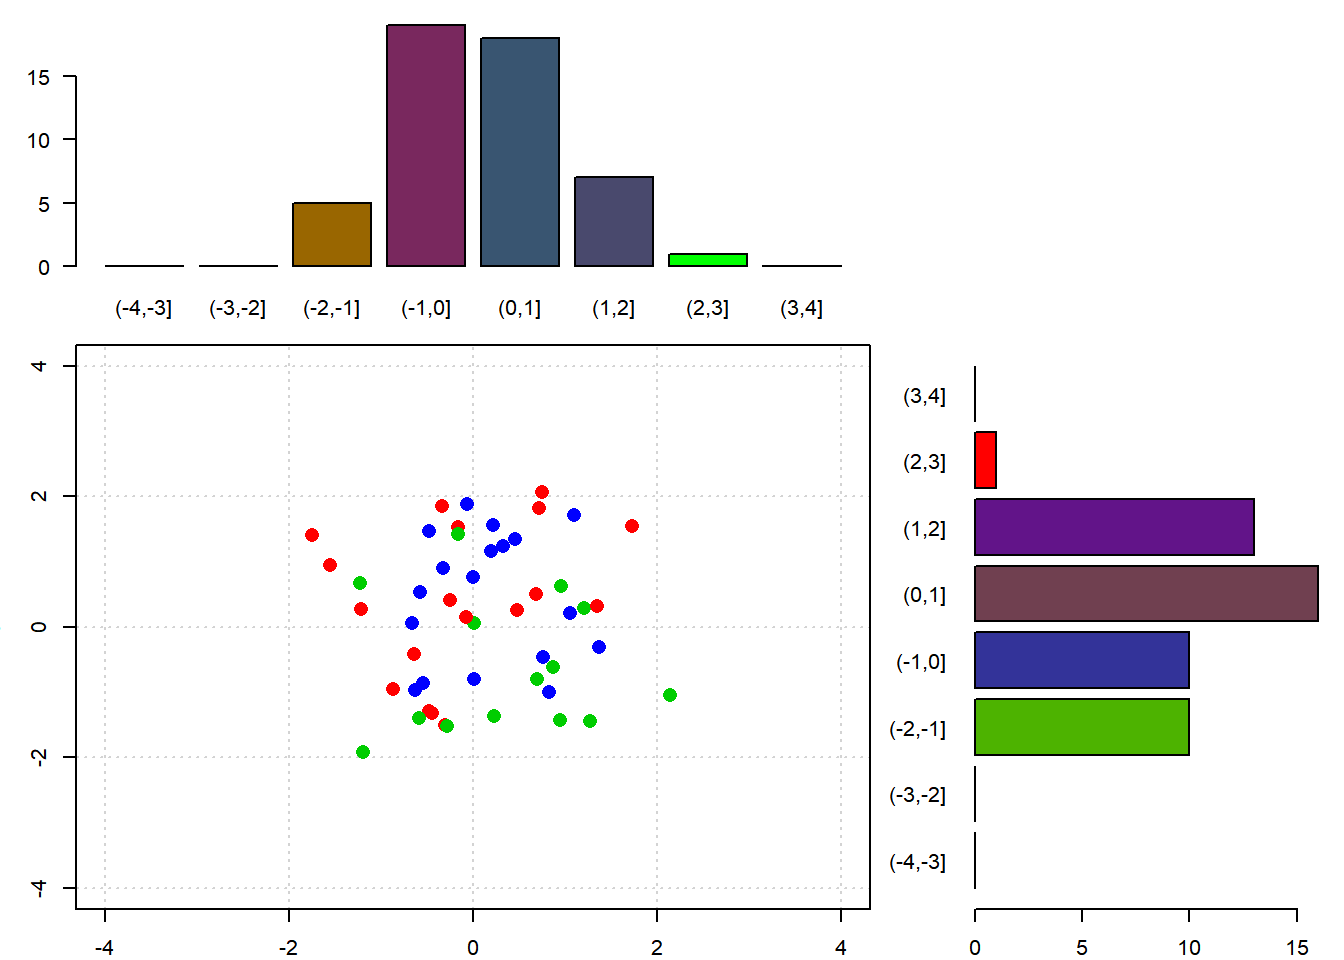
\includegraphics{myRBook_FR_files/figure-latex/unnamed-chunk-245-1.pdf}

Avec la fonction \texttt{rgb()} nous pouvons donc représenter \texttt{256\^{}3} couleurs, soit 167 777 216 couleurs différentes. Notre objectif reste cependant de faire des graphiques agréables à lire et qui mettent bien en valeurs nos résultats scientifiques. Il faut donc choisir les couleurs adéquates au regard de notre objectif. C'est pour cela que nous allons utiliser des palettes.

\hypertarget{palettes}{%
\section{Palettes}\label{palettes}}

Les palettes sont des jeux de couleurs représentées sous forme d'un \texttt{vector} avec les couleurs au format hexadécimal (valeur renvoyée par la fonction \texttt{rgb()} par exemple).

\begin{Shaded}
\begin{Highlighting}[]
\NormalTok{myPal <-}\StringTok{ }\KeywordTok{c}\NormalTok{(}
  \KeywordTok{rgb}\NormalTok{(}\DecValTok{0}\NormalTok{, }\DecValTok{94}\NormalTok{, }\DecValTok{255}\NormalTok{, }\DataTypeTok{maxColorValue =} \DecValTok{255}\NormalTok{),  }
  \KeywordTok{rgb}\NormalTok{(}\DecValTok{255}\NormalTok{, }\DecValTok{0}\NormalTok{, }\DecValTok{174}\NormalTok{, }\DataTypeTok{maxColorValue =} \DecValTok{255}\NormalTok{),  }
  \KeywordTok{rgb}\NormalTok{(}\DecValTok{255}\NormalTok{, }\DecValTok{136}\NormalTok{, }\DecValTok{0}\NormalTok{, }\DataTypeTok{maxColorValue =} \DecValTok{255}\NormalTok{),  }
  \KeywordTok{rgb}\NormalTok{(}\DecValTok{119}\NormalTok{, }\DecValTok{255}\NormalTok{, }\DecValTok{0}\NormalTok{, }\DataTypeTok{maxColorValue =} \DecValTok{255}\NormalTok{))}
\KeywordTok{print}\NormalTok{(myPal)}
\end{Highlighting}
\end{Shaded}

\begin{verbatim}
## [1] "#005EFF" "#FF00AE" "#FF8800" "#77FF00"
\end{verbatim}

\begin{Shaded}
\begin{Highlighting}[]
\KeywordTok{boxplot}\NormalTok{(}\KeywordTok{matrix}\NormalTok{(}\KeywordTok{rnorm}\NormalTok{(}\DecValTok{100}\NormalTok{), }\DataTypeTok{ncol =} \DecValTok{5}\NormalTok{), }\DataTypeTok{col =}\NormalTok{ myPal, }\DataTypeTok{axes =} \OtherTok{FALSE}\NormalTok{)}
\KeywordTok{axis}\NormalTok{(}\DecValTok{1}\NormalTok{)}
\KeywordTok{axis}\NormalTok{(}\DecValTok{2}\NormalTok{)}
\end{Highlighting}
\end{Shaded}

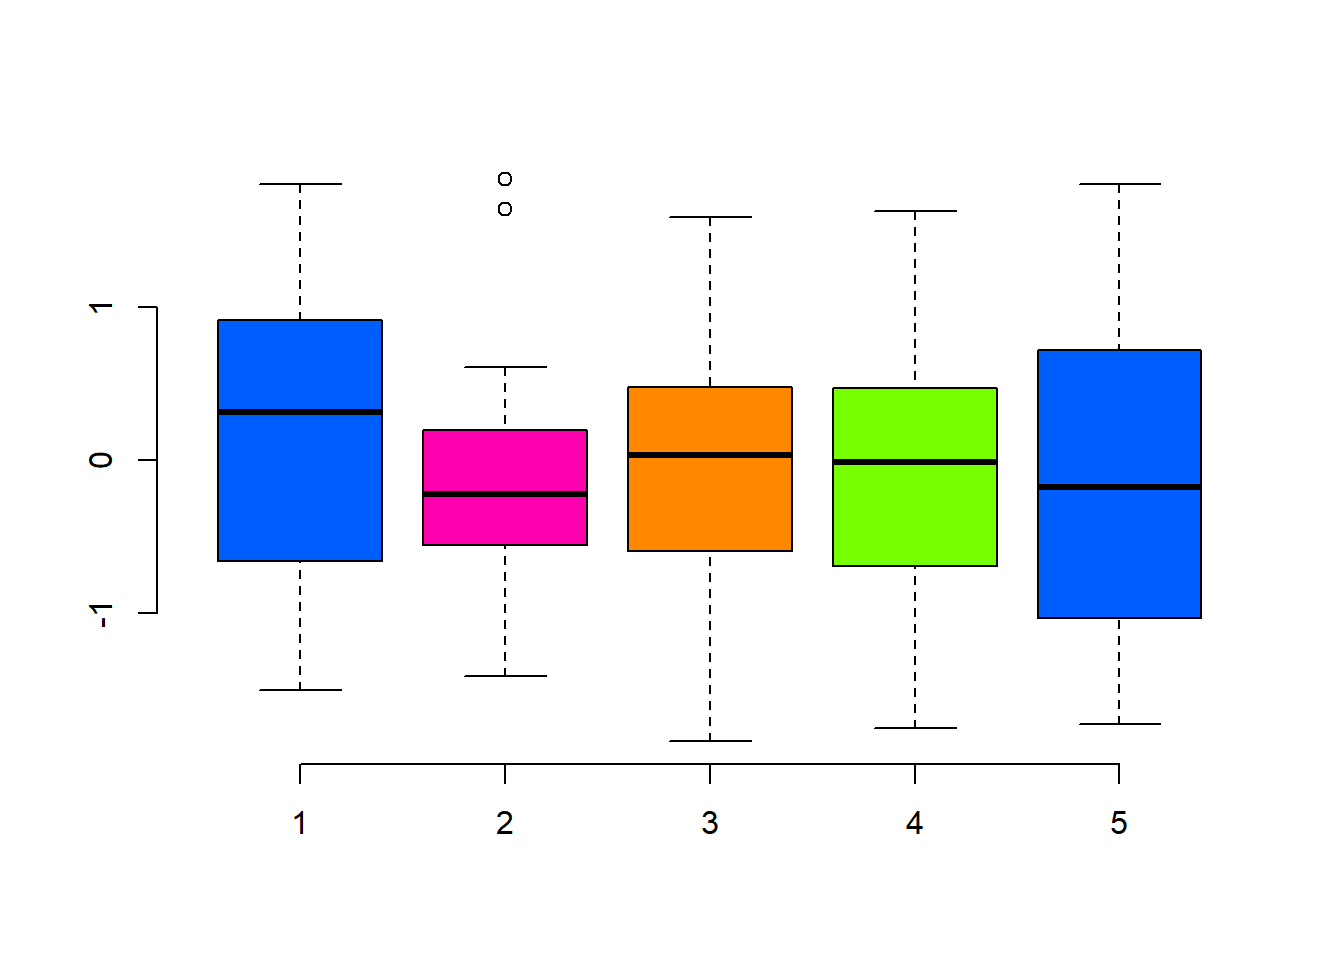
\includegraphics{myRBook_FR_files/figure-latex/unnamed-chunk-246-1.pdf}

Il existe des palettes inclues dans R : \texttt{terrain.colors()}, \texttt{heat.colors()}, \texttt{topo.colors()},
\texttt{cm.colors()}, \texttt{rainbow()}.

\begin{Shaded}
\begin{Highlighting}[]
\NormalTok{op <-}\StringTok{ }\KeywordTok{par}\NormalTok{(}\DataTypeTok{no.readonly =} \OtherTok{TRUE}\NormalTok{)}
\KeywordTok{par}\NormalTok{(}\DataTypeTok{mfrow =} \KeywordTok{c}\NormalTok{(}\DecValTok{2}\NormalTok{, }\DecValTok{3}\NormalTok{), }\DataTypeTok{mar =} \KeywordTok{c}\NormalTok{(}\DecValTok{0}\NormalTok{, }\DecValTok{0}\NormalTok{, }\DecValTok{2}\NormalTok{, }\DecValTok{0}\NormalTok{))}
\KeywordTok{boxplot}\NormalTok{(}\KeywordTok{matrix}\NormalTok{(}\KeywordTok{rnorm}\NormalTok{(}\DecValTok{1000}\NormalTok{), }\DataTypeTok{ncol =} \DecValTok{10}\NormalTok{), }\DataTypeTok{main =} \StringTok{"terrain.colors()"}\NormalTok{, }
  \DataTypeTok{col =} \KeywordTok{terrain.colors}\NormalTok{(}\DecValTok{10}\NormalTok{), }\DataTypeTok{axes =} \OtherTok{FALSE}\NormalTok{)}
\KeywordTok{boxplot}\NormalTok{(}\KeywordTok{matrix}\NormalTok{(}\KeywordTok{rnorm}\NormalTok{(}\DecValTok{1000}\NormalTok{), }\DataTypeTok{ncol =} \DecValTok{10}\NormalTok{), }\DataTypeTok{main =} \StringTok{"heat.colors()"}\NormalTok{, }
  \DataTypeTok{col =} \KeywordTok{heat.colors}\NormalTok{(}\DecValTok{10}\NormalTok{), }\DataTypeTok{axes =} \OtherTok{FALSE}\NormalTok{)}
\KeywordTok{boxplot}\NormalTok{(}\KeywordTok{matrix}\NormalTok{(}\KeywordTok{rnorm}\NormalTok{(}\DecValTok{1000}\NormalTok{), }\DataTypeTok{ncol =} \DecValTok{10}\NormalTok{), }\DataTypeTok{main =} \StringTok{"topo.colors()"}\NormalTok{, }
  \DataTypeTok{col =} \KeywordTok{topo.colors}\NormalTok{(}\DecValTok{10}\NormalTok{), }\DataTypeTok{axes =} \OtherTok{FALSE}\NormalTok{)}
\KeywordTok{boxplot}\NormalTok{(}\KeywordTok{matrix}\NormalTok{(}\KeywordTok{rnorm}\NormalTok{(}\DecValTok{1000}\NormalTok{), }\DataTypeTok{ncol =} \DecValTok{10}\NormalTok{), }\DataTypeTok{main =} \StringTok{"cm.colors()"}\NormalTok{, }
  \DataTypeTok{col =} \KeywordTok{cm.colors}\NormalTok{(}\DecValTok{10}\NormalTok{), }\DataTypeTok{axes =} \OtherTok{FALSE}\NormalTok{)}
\KeywordTok{boxplot}\NormalTok{(}\KeywordTok{matrix}\NormalTok{(}\KeywordTok{rnorm}\NormalTok{(}\DecValTok{1000}\NormalTok{), }\DataTypeTok{ncol =} \DecValTok{10}\NormalTok{), }\DataTypeTok{main =} \StringTok{"rainbow()"}\NormalTok{, }
  \DataTypeTok{col =} \KeywordTok{rainbow}\NormalTok{(}\DecValTok{10}\NormalTok{), }\DataTypeTok{axes =} \OtherTok{FALSE}\NormalTok{)}
\KeywordTok{par}\NormalTok{(op)}
\end{Highlighting}
\end{Shaded}

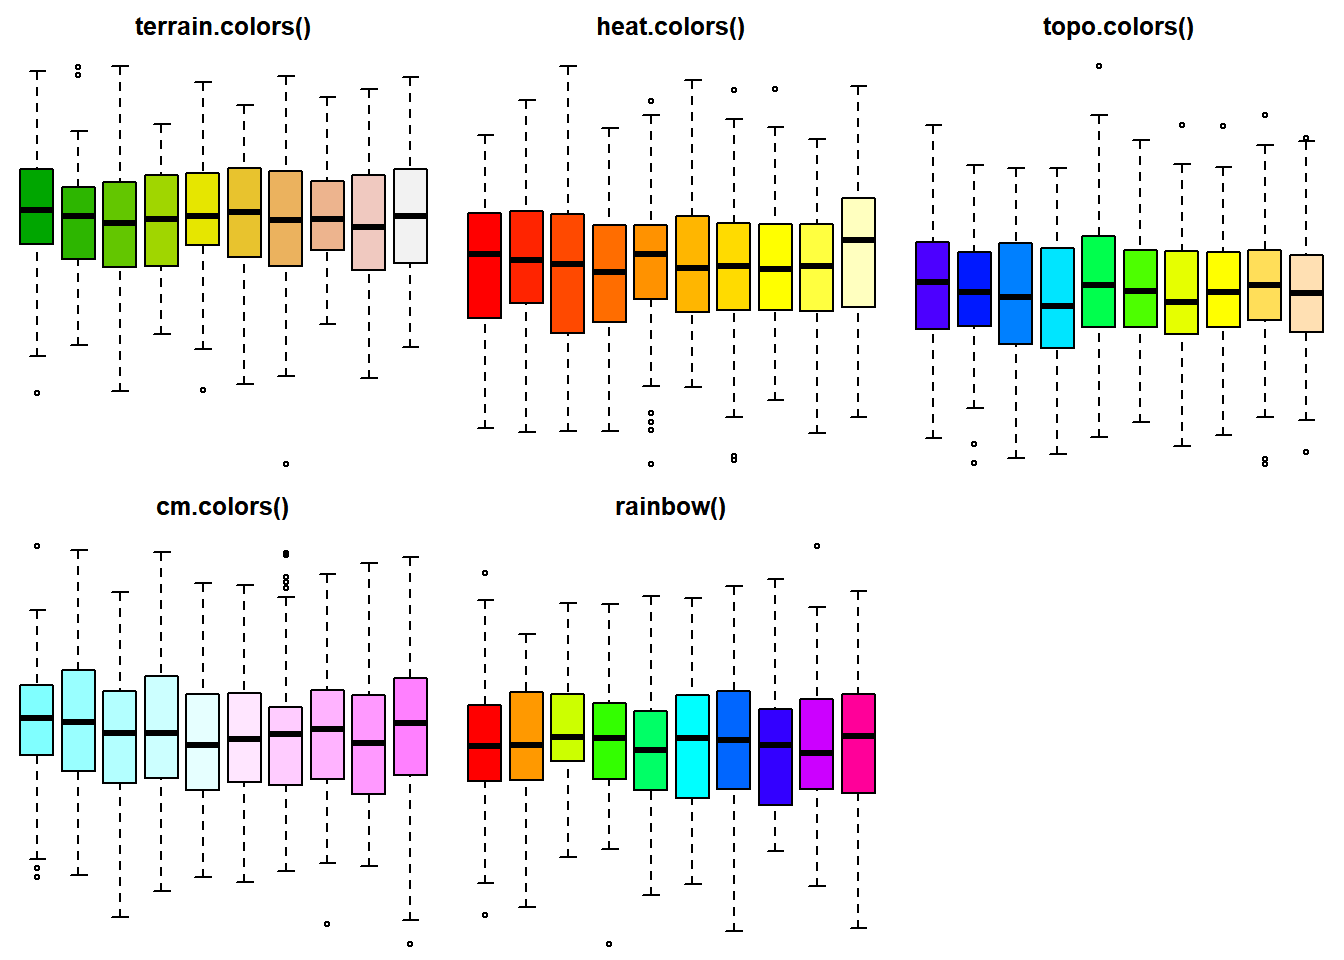
\includegraphics{myRBook_FR_files/figure-latex/unnamed-chunk-247-1.pdf}

Il existe aussi une fonction \texttt{colorRampPalette()} qui permet de créer un dégradé de couleur.

\begin{Shaded}
\begin{Highlighting}[]
\NormalTok{op <-}\StringTok{ }\KeywordTok{par}\NormalTok{(}\DataTypeTok{no.readonly =} \OtherTok{TRUE}\NormalTok{)}
\KeywordTok{par}\NormalTok{(}\DataTypeTok{mfrow =} \KeywordTok{c}\NormalTok{(}\DecValTok{3}\NormalTok{, }\DecValTok{1}\NormalTok{), }\DataTypeTok{mar =} \KeywordTok{c}\NormalTok{(}\DecValTok{0}\NormalTok{, }\DecValTok{0}\NormalTok{, }\DecValTok{0}\NormalTok{, }\DecValTok{0}\NormalTok{))}
\KeywordTok{boxplot}\NormalTok{(}\KeywordTok{matrix}\NormalTok{(}\KeywordTok{rnorm}\NormalTok{(}\DecValTok{2500}\NormalTok{), }\DataTypeTok{ncol =} \DecValTok{25}\NormalTok{), }
  \DataTypeTok{col =} \KeywordTok{colorRampPalette}\NormalTok{(}\KeywordTok{c}\NormalTok{(}\StringTok{'blue'}\NormalTok{, }\StringTok{'red'}\NormalTok{))(}\DecValTok{25}\NormalTok{), }\DataTypeTok{axes =} \OtherTok{FALSE}\NormalTok{)}
\KeywordTok{boxplot}\NormalTok{(}\KeywordTok{matrix}\NormalTok{(}\KeywordTok{rnorm}\NormalTok{(}\DecValTok{2500}\NormalTok{), }\DataTypeTok{ncol =} \DecValTok{25}\NormalTok{), }
  \DataTypeTok{col =} \KeywordTok{colorRampPalette}\NormalTok{(}\KeywordTok{c}\NormalTok{(}\StringTok{'blue'}\NormalTok{, }\StringTok{'white'}\NormalTok{, }\StringTok{'red'}\NormalTok{))(}\DecValTok{25}\NormalTok{), }\DataTypeTok{axes =} \OtherTok{FALSE}\NormalTok{)}
\KeywordTok{boxplot}\NormalTok{(}\KeywordTok{matrix}\NormalTok{(}\KeywordTok{rnorm}\NormalTok{(}\DecValTok{2500}\NormalTok{), }\DataTypeTok{ncol =} \DecValTok{25}\NormalTok{), }
  \DataTypeTok{col =}  \KeywordTok{colorRampPalette}\NormalTok{(}\KeywordTok{c}\NormalTok{(}\KeywordTok{rgb}\NormalTok{(}\DecValTok{255}\NormalTok{, }\DecValTok{136}\NormalTok{, }\DecValTok{0}\NormalTok{, }\DataTypeTok{maxColorValue =} \DecValTok{255}\NormalTok{),  }
  \KeywordTok{rgb}\NormalTok{(}\DecValTok{0}\NormalTok{, }\DecValTok{94}\NormalTok{, }\DecValTok{255}\NormalTok{, }\DataTypeTok{maxColorValue =} \DecValTok{255}\NormalTok{)))(}\DecValTok{25}\NormalTok{), }\DataTypeTok{axes =} \OtherTok{FALSE}\NormalTok{)}
\end{Highlighting}
\end{Shaded}

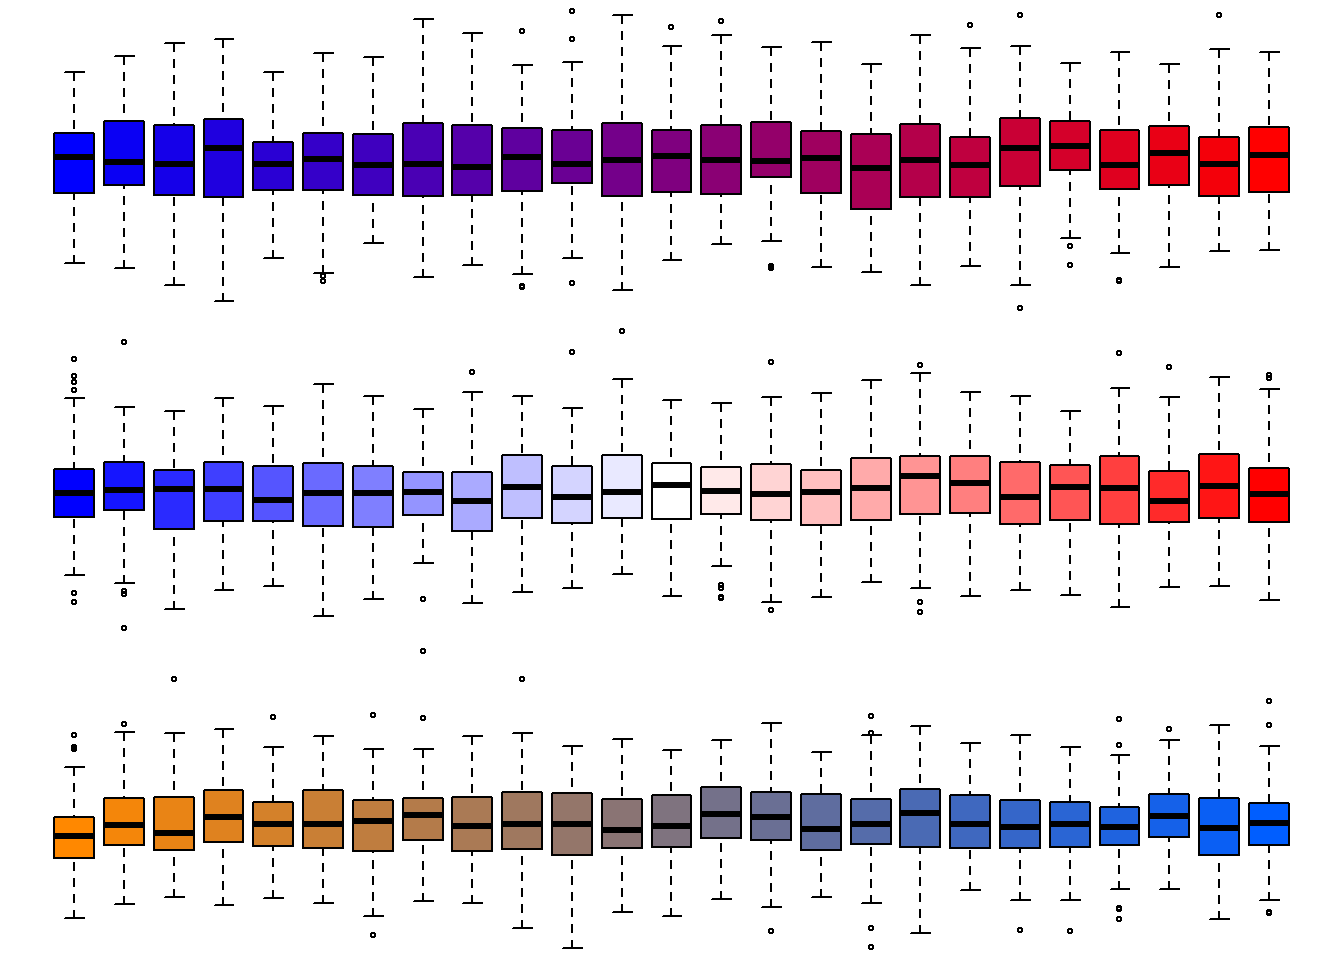
\includegraphics{myRBook_FR_files/figure-latex/unnamed-chunk-248-1.pdf}

\begin{Shaded}
\begin{Highlighting}[]
\KeywordTok{par}\NormalTok{(op)}
\end{Highlighting}
\end{Shaded}

Nous pouvons aussi créer nos propres palettes en utilisant des sites web dédiés à la sélection des couleurs comme \url{http://paletton.com/} ou \url{https://coolors.co/} (il en existe bien d'autres), puis les utiliser dans R en recopiant dans un vecteur les valeurs héxadécimales ou rgb.

R est un language de programmation très puissant. Nous pouvons imaginer de nombreuses façons de créer automatiquement des palettes en fonction de critères variés. Par exemple nous pouvons importer une image dont les teintes nous semblent pertinentes, puis extraire les informations de chacun des points pour ensuite sélectionner les couleurs dominantes via un regroupement par cluster. C'est ce que fait la fonction suivante.

Tout d'abord nous allons charger les packages \texttt{raster}, \texttt{rgdal} et \texttt{jpeg} qui vont nous servir à manipuler notre image sous R.

\begin{Shaded}
\begin{Highlighting}[]
\NormalTok{pkgCheck <-}\StringTok{ }\ControlFlowTok{function}\NormalTok{(x)\{ }
    \ControlFlowTok{if}\NormalTok{ (}\OperatorTok{!}\KeywordTok{require}\NormalTok{(x, }\DataTypeTok{character.only =} \OtherTok{TRUE}\NormalTok{))\{}
        \KeywordTok{install.packages}\NormalTok{(x, }\DataTypeTok{dependencies =} \OtherTok{TRUE}\NormalTok{)}
        \ControlFlowTok{if}\NormalTok{(}\OperatorTok{!}\KeywordTok{require}\NormalTok{(x, }\DataTypeTok{character.only =} \OtherTok{TRUE}\NormalTok{)) \{}
            \KeywordTok{stop}\NormalTok{()}
\NormalTok{        \}}
\NormalTok{    \}}
\NormalTok{\}}
\KeywordTok{pkgCheck}\NormalTok{(}\StringTok{"raster"}\NormalTok{)}
\KeywordTok{pkgCheck}\NormalTok{(}\StringTok{"rgdal"}\NormalTok{)}
\KeywordTok{pkgCheck}\NormalTok{(}\StringTok{"jpeg"}\NormalTok{)}
\end{Highlighting}
\end{Shaded}

Ensuite nous allons utiliser la fonction \texttt{kmeans()} pour effectuer des groupes de couleurs en utilisant les valeurs RGB de chacun des points de notre image. Ici nous avons deux méthodes possibles, la première utilise la fonction \texttt{kmeans()} pour les trois valeurs RGB, et la seconde utilise la fonction \texttt{kmeans()} pour chaque valeur RGB individuellement (cette seconde fonction donne une palette qui pourra être assez éloignée des couleurs de l'image de départ).

\begin{Shaded}
\begin{Highlighting}[]
\NormalTok{createPal <-}\StringTok{ }\ControlFlowTok{function}\NormalTok{(photo, }\DataTypeTok{met =} \DecValTok{1}\NormalTok{, }\DataTypeTok{graph =} \OtherTok{TRUE}\NormalTok{, }\DataTypeTok{k =} \DecValTok{9}\NormalTok{)\{}
    \ControlFlowTok{if}\NormalTok{(met }\OperatorTok{==}\StringTok{ }\DecValTok{1}\NormalTok{)\{}
\NormalTok{        colR <-}\StringTok{ }\KeywordTok{getValues}\NormalTok{(}\KeywordTok{raster}\NormalTok{(photo, }\DataTypeTok{band =} \DecValTok{1}\NormalTok{))}
\NormalTok{        colG <-}\StringTok{ }\KeywordTok{getValues}\NormalTok{(}\KeywordTok{raster}\NormalTok{(photo, }\DataTypeTok{band =} \DecValTok{2}\NormalTok{))}
\NormalTok{        colB <-}\StringTok{ }\KeywordTok{getValues}\NormalTok{(}\KeywordTok{raster}\NormalTok{(photo, }\DataTypeTok{band =} \DecValTok{3}\NormalTok{))}
\NormalTok{        kMeans <-}\StringTok{ }\KeywordTok{kmeans}\NormalTok{(}\KeywordTok{data.frame}\NormalTok{(colR, colG, colB), }\DataTypeTok{centers =}\NormalTok{ k)}
\NormalTok{        kCol <-}\StringTok{ }\KeywordTok{rgb}\NormalTok{(kMeans}\OperatorTok{$}\NormalTok{centers, }\DataTypeTok{maxColorValue =} \DecValTok{255}\NormalTok{)[}\KeywordTok{order}\NormalTok{(}\KeywordTok{table}\NormalTok{(}
\NormalTok{            kMeans}\OperatorTok{$}\NormalTok{cluster), }\DataTypeTok{decreasing =} \OtherTok{TRUE}\NormalTok{)]}
        \ControlFlowTok{if}\NormalTok{(graph }\OperatorTok{==}\StringTok{ }\OtherTok{TRUE}\NormalTok{)\{}
\NormalTok{          op <-}\StringTok{ }\KeywordTok{par}\NormalTok{(}\DataTypeTok{no.readonly =} \OtherTok{TRUE}\NormalTok{)}
          \KeywordTok{par}\NormalTok{(}\DataTypeTok{mfrow =} \KeywordTok{c}\NormalTok{ (}\DecValTok{1}\NormalTok{, }\DecValTok{2}\NormalTok{), }\DataTypeTok{mar =} \KeywordTok{c}\NormalTok{(}\DecValTok{0}\NormalTok{, }\DecValTok{2}\NormalTok{, }\DecValTok{2}\NormalTok{, }\DecValTok{0}\NormalTok{))}
\NormalTok{          myJpg <-}\StringTok{ }\KeywordTok{readJPEG}\NormalTok{(}\StringTok{"./myFiles/photoKmeans.jpg"}\NormalTok{, }\DataTypeTok{native =} \OtherTok{TRUE}\NormalTok{)}
          \KeywordTok{plot}\NormalTok{(}\DecValTok{0}\OperatorTok{:}\DecValTok{1}\NormalTok{, }\DecValTok{0}\OperatorTok{:}\DecValTok{1}\NormalTok{, }\DataTypeTok{type =} \StringTok{"n"}\NormalTok{, }\DataTypeTok{ann =} \OtherTok{FALSE}\NormalTok{, }\DataTypeTok{axes =} \OtherTok{FALSE}\NormalTok{)}
          \KeywordTok{rasterImage}\NormalTok{(myJpg, }\DecValTok{0}\NormalTok{, }\DecValTok{0}\NormalTok{, }\DecValTok{1}\NormalTok{, }\DecValTok{1}\NormalTok{)}
          \KeywordTok{barplot}\NormalTok{(}\KeywordTok{table}\NormalTok{(kMeans}\OperatorTok{$}\NormalTok{cluster)[}\KeywordTok{order}\NormalTok{(}\KeywordTok{table}\NormalTok{(kMeans}\OperatorTok{$}\NormalTok{cluster), }
            \DataTypeTok{decreasing =} \OtherTok{TRUE}\NormalTok{)], }\DataTypeTok{col =}\NormalTok{ kCol, }\DataTypeTok{names.arg =} \OtherTok{NA}\NormalTok{)}
          \KeywordTok{par}\NormalTok{(op)}
\NormalTok{        \}}
        \KeywordTok{return}\NormalTok{(kCol)}
\NormalTok{    \} }\ControlFlowTok{else}\NormalTok{ \{}
        \ControlFlowTok{if}\NormalTok{(met }\OperatorTok{==}\StringTok{ }\DecValTok{2}\NormalTok{)\{}
\NormalTok{            kColR <-}\StringTok{ }\KeywordTok{kmeans}\NormalTok{(}\DataTypeTok{x =} \KeywordTok{getValues}\NormalTok{(}\KeywordTok{raster}\NormalTok{(photo, }\DataTypeTok{band =} \DecValTok{1}\NormalTok{)), }
                \DataTypeTok{centers =}\NormalTok{ k)}
\NormalTok{            kColG <-}\StringTok{ }\KeywordTok{kmeans}\NormalTok{(}\DataTypeTok{x =} \KeywordTok{getValues}\NormalTok{(}\KeywordTok{raster}\NormalTok{(photo, }\DataTypeTok{band =} \DecValTok{2}\NormalTok{)), }
                \DataTypeTok{centers =}\NormalTok{ k)}
\NormalTok{            kColB <-}\StringTok{ }\KeywordTok{kmeans}\NormalTok{(}\DataTypeTok{x =} \KeywordTok{getValues}\NormalTok{(}\KeywordTok{raster}\NormalTok{(photo, }\DataTypeTok{band =} \DecValTok{3}\NormalTok{)), }
                \DataTypeTok{centers =}\NormalTok{ k)}
\NormalTok{            kCol <-}\StringTok{ }\NormalTok{(}\KeywordTok{rgb}\NormalTok{(kColR}\OperatorTok{$}\NormalTok{centers, kColG}\OperatorTok{$}\NormalTok{centers, kColB}\OperatorTok{$}\NormalTok{centers,}
                \DataTypeTok{maxColorValue =} \DecValTok{255}\NormalTok{))}
            \ControlFlowTok{if}\NormalTok{(graph }\OperatorTok{==}\StringTok{ }\OtherTok{TRUE}\NormalTok{)\{}
\NormalTok{                op <-}\StringTok{ }\KeywordTok{par}\NormalTok{(}\DataTypeTok{no.readonly =} \OtherTok{TRUE}\NormalTok{)}
                \KeywordTok{par}\NormalTok{(}\DataTypeTok{mfrow =} \KeywordTok{c}\NormalTok{ (}\DecValTok{1}\NormalTok{, }\DecValTok{2}\NormalTok{), }\DataTypeTok{mar =} \KeywordTok{c}\NormalTok{(}\DecValTok{0}\NormalTok{, }\DecValTok{2}\NormalTok{, }\DecValTok{2}\NormalTok{, }\DecValTok{0}\NormalTok{))}
\NormalTok{                myJpg <-}\StringTok{ }\KeywordTok{readJPEG}\NormalTok{(}\StringTok{"./myFiles/photoKmeans.jpg"}\NormalTok{, }\DataTypeTok{native =} \OtherTok{TRUE}\NormalTok{)}
                \KeywordTok{plot}\NormalTok{(}\DecValTok{0}\OperatorTok{:}\DecValTok{1}\NormalTok{, }\DecValTok{0}\OperatorTok{:}\DecValTok{1}\NormalTok{, }\DataTypeTok{type =} \StringTok{"n"}\NormalTok{, }\DataTypeTok{ann =} \OtherTok{FALSE}\NormalTok{, }\DataTypeTok{axes =} \OtherTok{FALSE}\NormalTok{)}
                \KeywordTok{rasterImage}\NormalTok{(myJpg, }\DecValTok{0}\NormalTok{, }\DecValTok{0}\NormalTok{, }\DecValTok{1}\NormalTok{, }\DecValTok{1}\NormalTok{)}
                \CommentTok{# par(mar = c(0, 0, 0, 0))}
                \KeywordTok{plot}\NormalTok{(}\DataTypeTok{x =} \DecValTok{1}\OperatorTok{:}\NormalTok{k, }\DataTypeTok{y =} \KeywordTok{rep}\NormalTok{(}\DecValTok{1}\NormalTok{, k), }\DataTypeTok{ylim =} \KeywordTok{c}\NormalTok{(}\DecValTok{0}\NormalTok{, }\DecValTok{1}\NormalTok{), }
                    \DataTypeTok{xlim =} \KeywordTok{c}\NormalTok{(}\DecValTok{0}\NormalTok{, k), }\DataTypeTok{axes =} \OtherTok{FALSE}\NormalTok{, }\DataTypeTok{xlab =} \StringTok{""}\NormalTok{, }
                    \DataTypeTok{ylab =} \StringTok{""}\NormalTok{, }\DataTypeTok{type =} \StringTok{"n"}\NormalTok{)}
                \ControlFlowTok{for}\NormalTok{(i }\ControlFlowTok{in} \DecValTok{1}\OperatorTok{:}\NormalTok{k)\{}
                    \KeywordTok{polygon}\NormalTok{(}\DataTypeTok{x =} \KeywordTok{c}\NormalTok{(i}\DecValTok{-1}\NormalTok{, i, i, i}\DecValTok{-1}\NormalTok{), }\DataTypeTok{y =} \KeywordTok{c}\NormalTok{(}\DecValTok{0}\NormalTok{, }\DecValTok{0}\NormalTok{, }\DecValTok{1}\NormalTok{, }\DecValTok{1}\NormalTok{), }
                        \DataTypeTok{col =}\NormalTok{ kCol[i])}
                    \KeywordTok{text}\NormalTok{(}\DataTypeTok{x =}\NormalTok{ i }\OperatorTok{-}\StringTok{ }\FloatTok{0.5}\NormalTok{, }\DataTypeTok{y =} \FloatTok{0.5}\NormalTok{, }
                        \DataTypeTok{labels =} \KeywordTok{as.character}\NormalTok{(kCol[i]), }\DataTypeTok{srt =} \DecValTok{90}\NormalTok{)}
\NormalTok{                \}}
                \KeywordTok{par}\NormalTok{(op)}
\NormalTok{            \}}
            \KeywordTok{return}\NormalTok{(kCol)}
\NormalTok{        \} }\ControlFlowTok{else}\NormalTok{ \{}
            \KeywordTok{print}\NormalTok{(}\KeywordTok{paste0}\NormalTok{(}\StringTok{"No method "}\NormalTok{, met, }\StringTok{"."}\NormalTok{))}
            \KeywordTok{return}\NormalTok{(}\KeywordTok{rgb}\NormalTok{(}\DecValTok{0}\NormalTok{, }\DecValTok{0}\NormalTok{, }\DecValTok{0}\NormalTok{))}
\NormalTok{        \}}
\NormalTok{    \}}
\NormalTok{\}}

\NormalTok{myPalMet1 <-}\StringTok{ }\KeywordTok{createPal}\NormalTok{(}\DataTypeTok{photo =} \StringTok{"./myFiles/photoKmeans.jpg"}\NormalTok{, }
  \DataTypeTok{met =} \DecValTok{1}\NormalTok{, }\DataTypeTok{graph =} \OtherTok{TRUE}\NormalTok{, }\DataTypeTok{k =} \DecValTok{5}\NormalTok{)}
\end{Highlighting}
\end{Shaded}

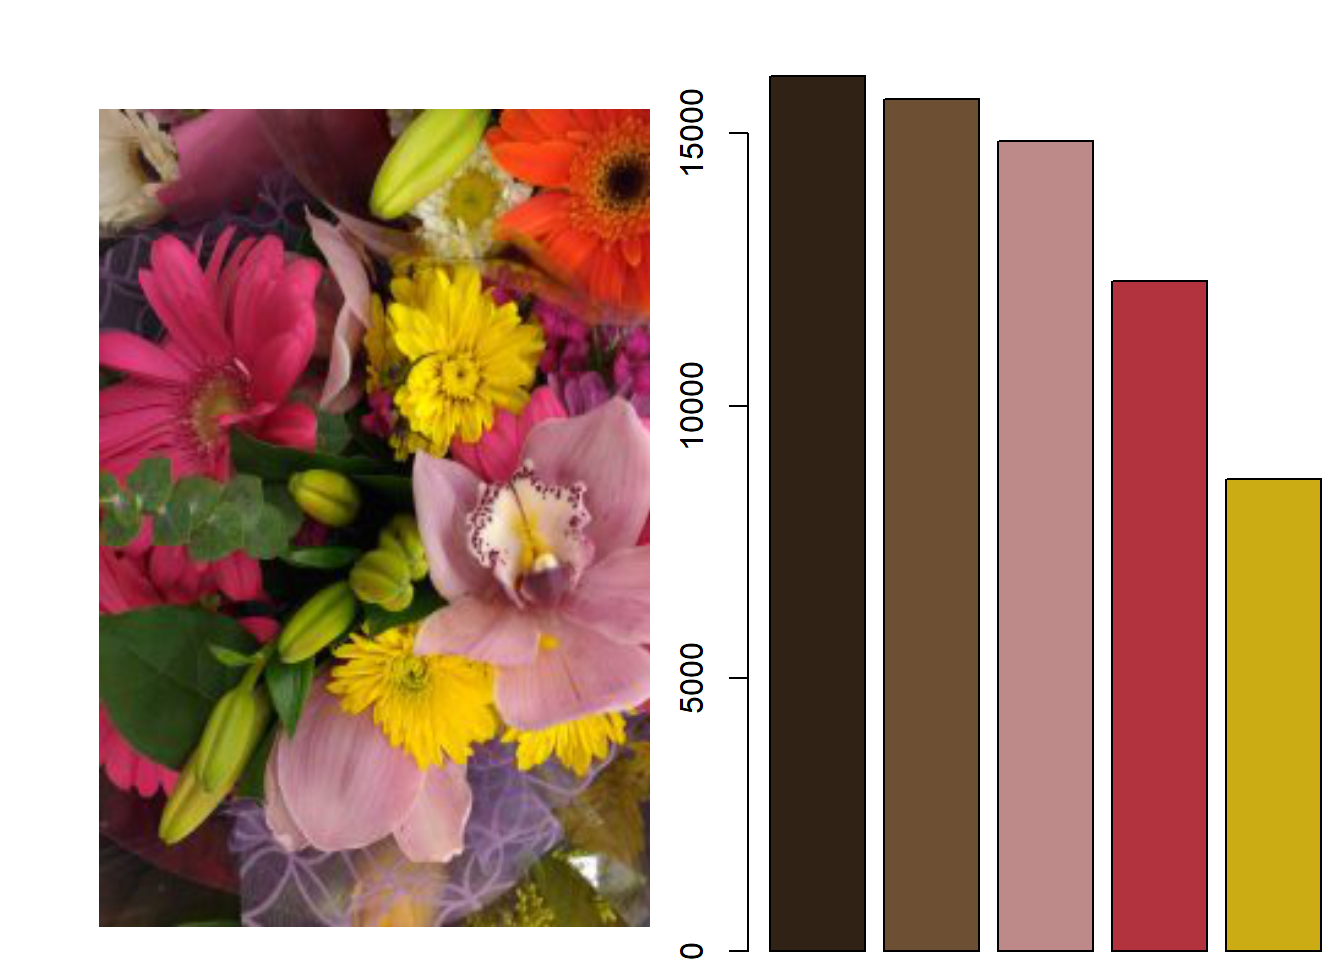
\includegraphics{myRBook_FR_files/figure-latex/unnamed-chunk-250-1.pdf}

\begin{Shaded}
\begin{Highlighting}[]
\NormalTok{myPalMet2 <-}\StringTok{ }\KeywordTok{createPal}\NormalTok{(}\DataTypeTok{photo =} \StringTok{"./myFiles/photoKmeans.jpg"}\NormalTok{, }
  \DataTypeTok{met =} \DecValTok{2}\NormalTok{, }\DataTypeTok{graph =} \OtherTok{TRUE}\NormalTok{, }\DataTypeTok{k =} \DecValTok{5}\NormalTok{)}
\end{Highlighting}
\end{Shaded}

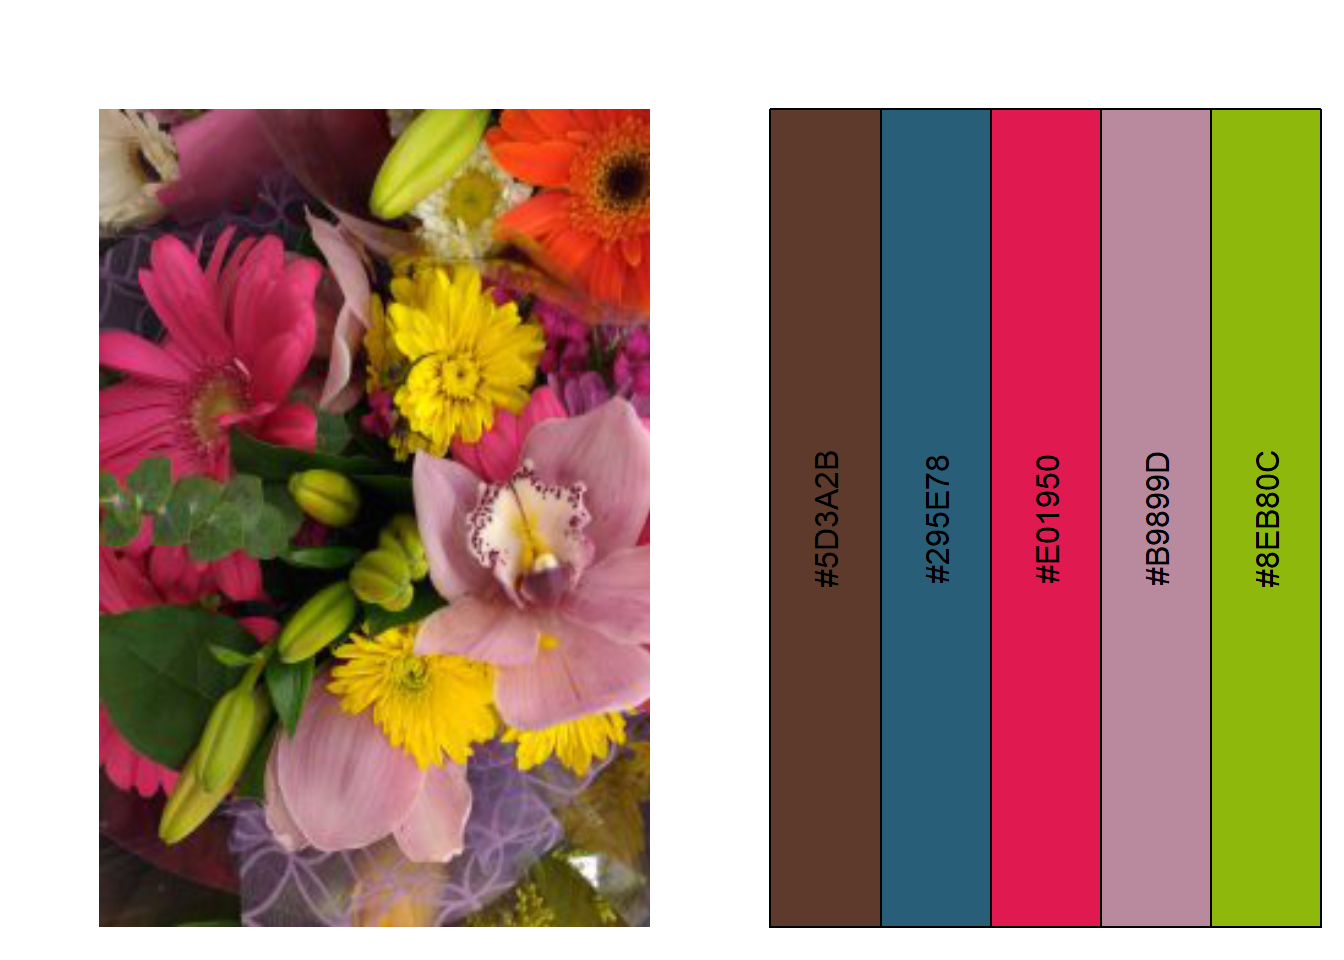
\includegraphics{myRBook_FR_files/figure-latex/unnamed-chunk-250-2.pdf}

La fonction nous renvoie les couleurs de la palette avec un graphique en barres représentant le nombre de points de l'image dans chacun des groupes de couleurs. Nous pouvons désormais utiliser notre nouvelle palette pour réaliser nos graphiques.

\begin{Shaded}
\begin{Highlighting}[]
\NormalTok{makeImpact <-}\StringTok{ }\ControlFlowTok{function}\NormalTok{(myPal, }\DataTypeTok{numP =} \DecValTok{300}\NormalTok{, }\DataTypeTok{impact =} \FloatTok{0.33}\NormalTok{, }\DataTypeTok{multCex =} \DecValTok{3}\NormalTok{)\{}
\NormalTok{    myX <-}\StringTok{ }\KeywordTok{sample}\NormalTok{(}\DecValTok{0}\OperatorTok{:}\DecValTok{1000}\NormalTok{, }\DataTypeTok{size =}\NormalTok{ numP, }\DataTypeTok{replace =} \OtherTok{TRUE}\NormalTok{)}\OperatorTok{/}\DecValTok{1000}
\NormalTok{    myY <-}\StringTok{ }\KeywordTok{sample}\NormalTok{(}\DecValTok{0}\OperatorTok{:}\DecValTok{1000}\NormalTok{, }\DataTypeTok{size =}\NormalTok{ numP, }\DataTypeTok{replace =} \OtherTok{TRUE}\NormalTok{)}\OperatorTok{/}\DecValTok{1000}
\NormalTok{    distImpact <-}\StringTok{ }\KeywordTok{sqrt}\NormalTok{((myX }\OperatorTok{-}\StringTok{ }\NormalTok{impact)}\OperatorTok{^}\DecValTok{2} \OperatorTok{+}\StringTok{ }\NormalTok{(myY }\OperatorTok{-}\StringTok{ }\NormalTok{impact)}\OperatorTok{^}\DecValTok{2}\NormalTok{)}
\NormalTok{    dfXY <-}\StringTok{ }\KeywordTok{data.frame}\NormalTok{(myX, myY, distImpact)}
    \KeywordTok{plot}\NormalTok{(}\DataTypeTok{x =}\NormalTok{ dfXY}\OperatorTok{$}\NormalTok{myX, }\DataTypeTok{y =}\NormalTok{ dfXY}\OperatorTok{$}\NormalTok{myY, }\DataTypeTok{axes =} \OtherTok{FALSE}\NormalTok{, }
        \DataTypeTok{xlab =} \StringTok{""}\NormalTok{, }\DataTypeTok{ylab =} \StringTok{""}\NormalTok{, }\DataTypeTok{cex =}\NormalTok{ dfXY}\OperatorTok{$}\NormalTok{distImpact}\OperatorTok{*}\NormalTok{multCex, }
        \DataTypeTok{col =}\NormalTok{ myPal, }\DataTypeTok{pch =} \DecValTok{16}\NormalTok{)}
\NormalTok{\}}

\NormalTok{op <-}\StringTok{ }\KeywordTok{par}\NormalTok{(}\DataTypeTok{no.readonly =} \OtherTok{TRUE}\NormalTok{)}
\KeywordTok{par}\NormalTok{(}\DataTypeTok{mfrow =} \KeywordTok{c}\NormalTok{ (}\DecValTok{1}\NormalTok{, }\DecValTok{2}\NormalTok{), }\DataTypeTok{mar =} \KeywordTok{c}\NormalTok{(}\DecValTok{0}\NormalTok{, }\DecValTok{0}\NormalTok{, }\DecValTok{0}\NormalTok{, }\DecValTok{0}\NormalTok{))}
\KeywordTok{makeImpact}\NormalTok{(}\DataTypeTok{myPal =}\NormalTok{ myPalMet1, }\DataTypeTok{numP =} \DecValTok{3000}\NormalTok{, }\DataTypeTok{impact =} \FloatTok{0.33}\NormalTok{)}
\KeywordTok{makeImpact}\NormalTok{(}\DataTypeTok{myPal =}\NormalTok{ myPalMet2, }\DataTypeTok{numP =} \DecValTok{3000}\NormalTok{, }\DataTypeTok{impact =} \FloatTok{0.66}\NormalTok{)}
\end{Highlighting}
\end{Shaded}

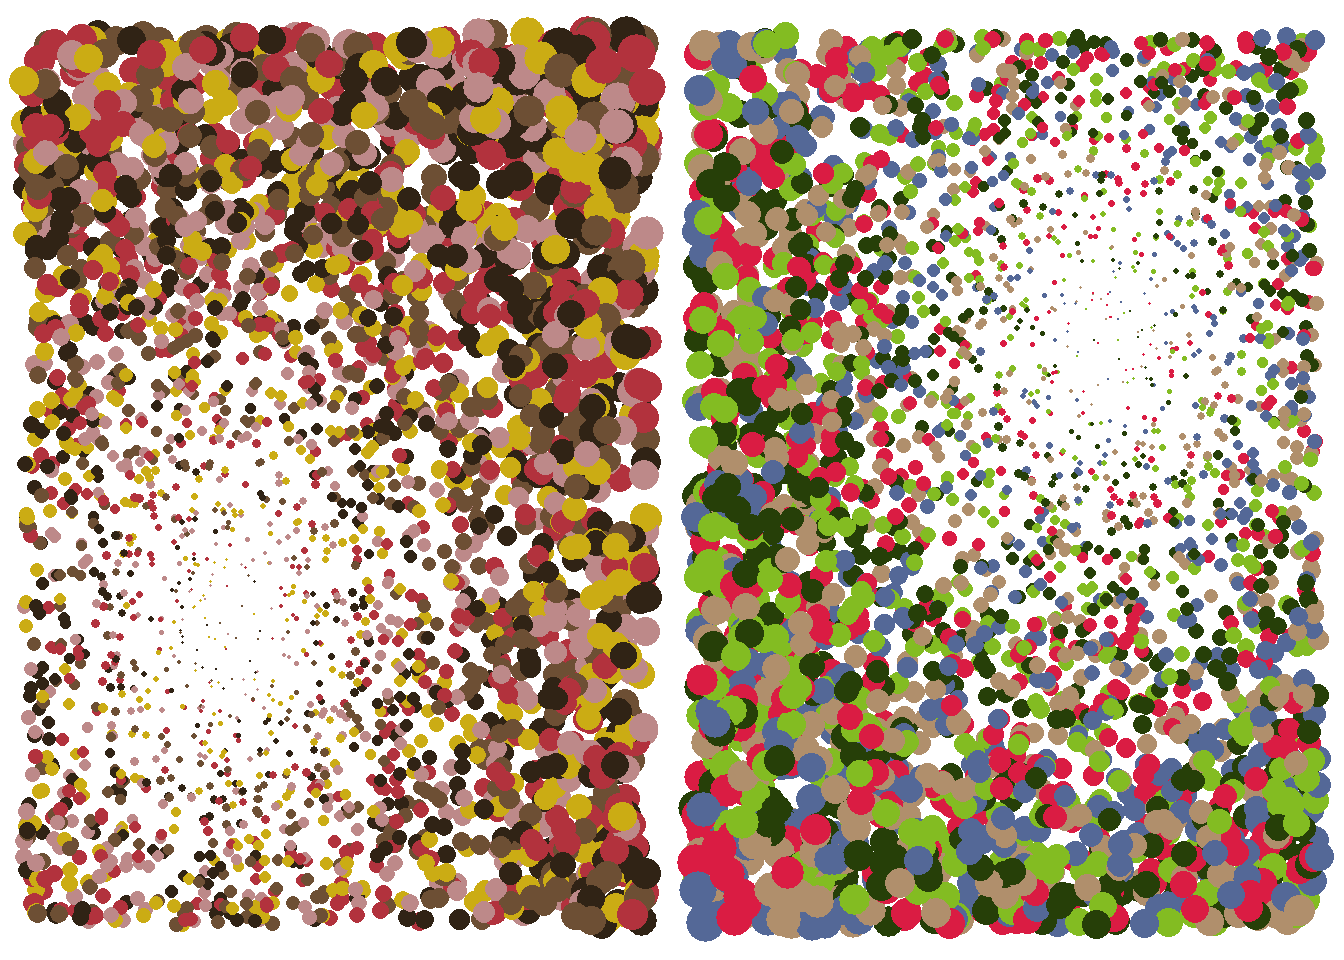
\includegraphics{myRBook_FR_files/figure-latex/unnamed-chunk-251-1.pdf}

\begin{Shaded}
\begin{Highlighting}[]
\KeywordTok{par}\NormalTok{(op)}
\end{Highlighting}
\end{Shaded}

\hypertarget{conclusion-9}{%
\section{Conclusion}\label{conclusion-9}}

Félicitations ! C'est la fin de ce chapitre sur la gestion des couleurs. Nous savons désormais comment utiliser les couleurs et les palettes, et comment guider le choix des couleurs pour mettre en valeur nos résultats. Dans le prochain chapitre nous allons voir quelques exemples de packages graphiques et les dernières tendances comme les graphiques dynamiques.

\hypertarget{graph3}{%
\chapter{Les packages graphiques}\label{graph3}}

\hypertarget{les-packages-de-palettes}{%
\section{les packages de palettes}\label{les-packages-de-palettes}}

\hypertarget{rcolorbrewer}{%
\subsection{\texorpdfstring{\texttt{RColorBrewer}}{RColorBrewer}}\label{rcolorbrewer}}

Le package \texttt{RColorBrewer} est un package populaire qui contient des palettes complémentaires à celle disponibles dans la version de base de R. Une fois le package installé, il suffit d'appeler les palettes pour les utiliser. Voici les palettes disponibles et un exemple d'utilisation.

\begin{Shaded}
\begin{Highlighting}[]
\NormalTok{pkgCheck <-}\StringTok{ }\ControlFlowTok{function}\NormalTok{(x)\{ }
    \ControlFlowTok{if}\NormalTok{ (}\OperatorTok{!}\KeywordTok{require}\NormalTok{(x, }\DataTypeTok{character.only =} \OtherTok{TRUE}\NormalTok{))\{}
        \KeywordTok{install.packages}\NormalTok{(x, }\DataTypeTok{dependencies =} \OtherTok{TRUE}\NormalTok{)}
        \ControlFlowTok{if}\NormalTok{(}\OperatorTok{!}\KeywordTok{require}\NormalTok{(x, }\DataTypeTok{character.only =} \OtherTok{TRUE}\NormalTok{)) \{}
            \KeywordTok{stop}\NormalTok{()}
\NormalTok{        \}}
\NormalTok{    \}}
\NormalTok{\}}
\KeywordTok{pkgCheck}\NormalTok{(}\StringTok{"RColorBrewer"}\NormalTok{)}
\KeywordTok{display.brewer.all}\NormalTok{()}
\end{Highlighting}
\end{Shaded}

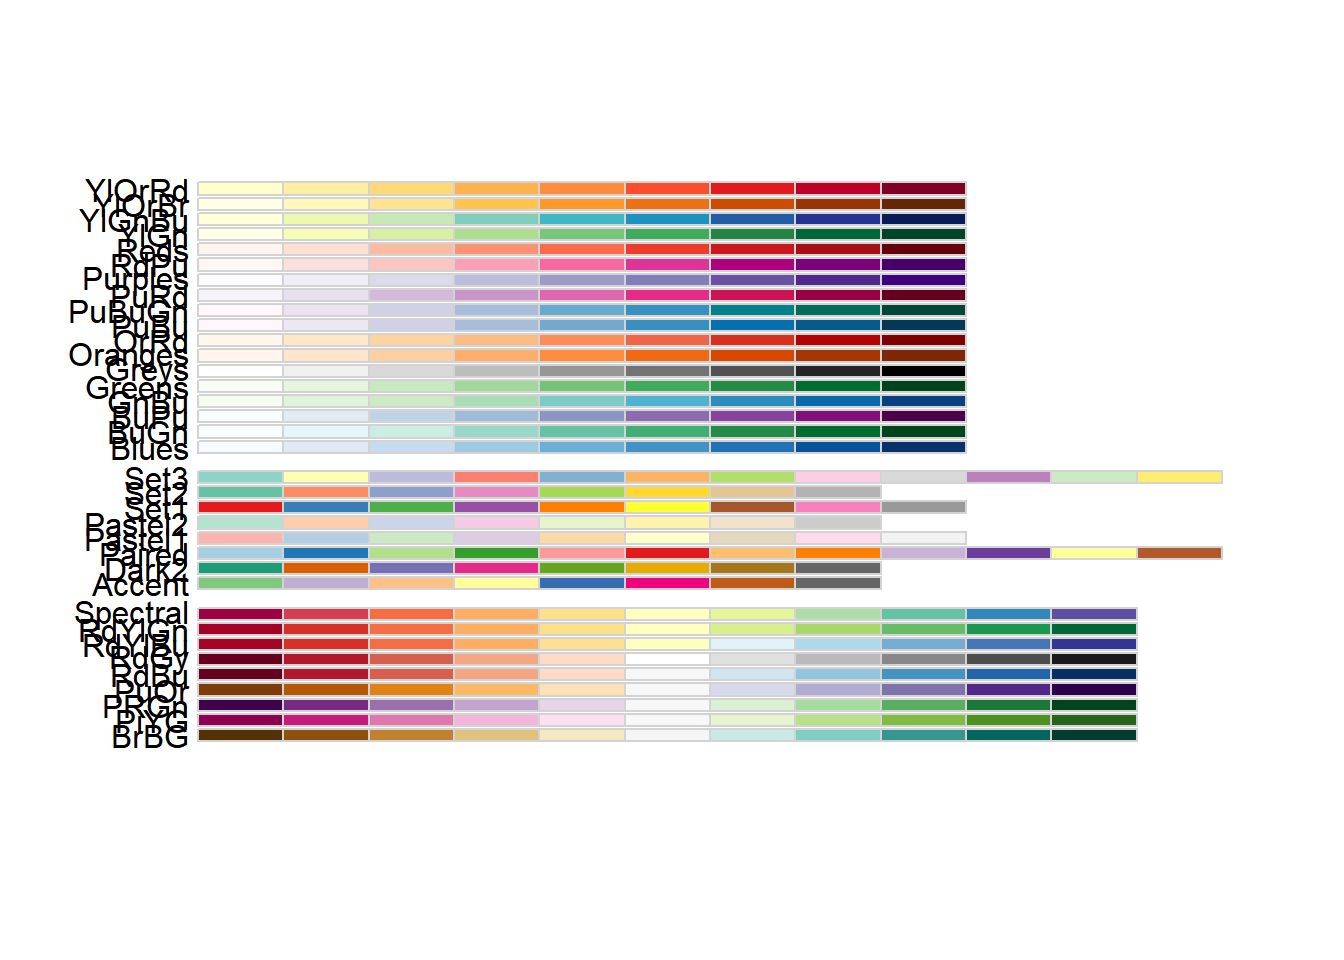
\includegraphics{myRBook_FR_files/figure-latex/unnamed-chunk-252-1.pdf}

\begin{Shaded}
\begin{Highlighting}[]
\KeywordTok{boxplot}\NormalTok{(}\KeywordTok{matrix}\NormalTok{(}\KeywordTok{rnorm}\NormalTok{(}\DecValTok{1000}\NormalTok{), }\DataTypeTok{ncol =} \DecValTok{10}\NormalTok{), }
  \DataTypeTok{col =} \KeywordTok{brewer.pal}\NormalTok{(}\DecValTok{10}\NormalTok{, }\StringTok{"Paired"}\NormalTok{), }\DataTypeTok{axes =} \OtherTok{FALSE}\NormalTok{)}
\end{Highlighting}
\end{Shaded}

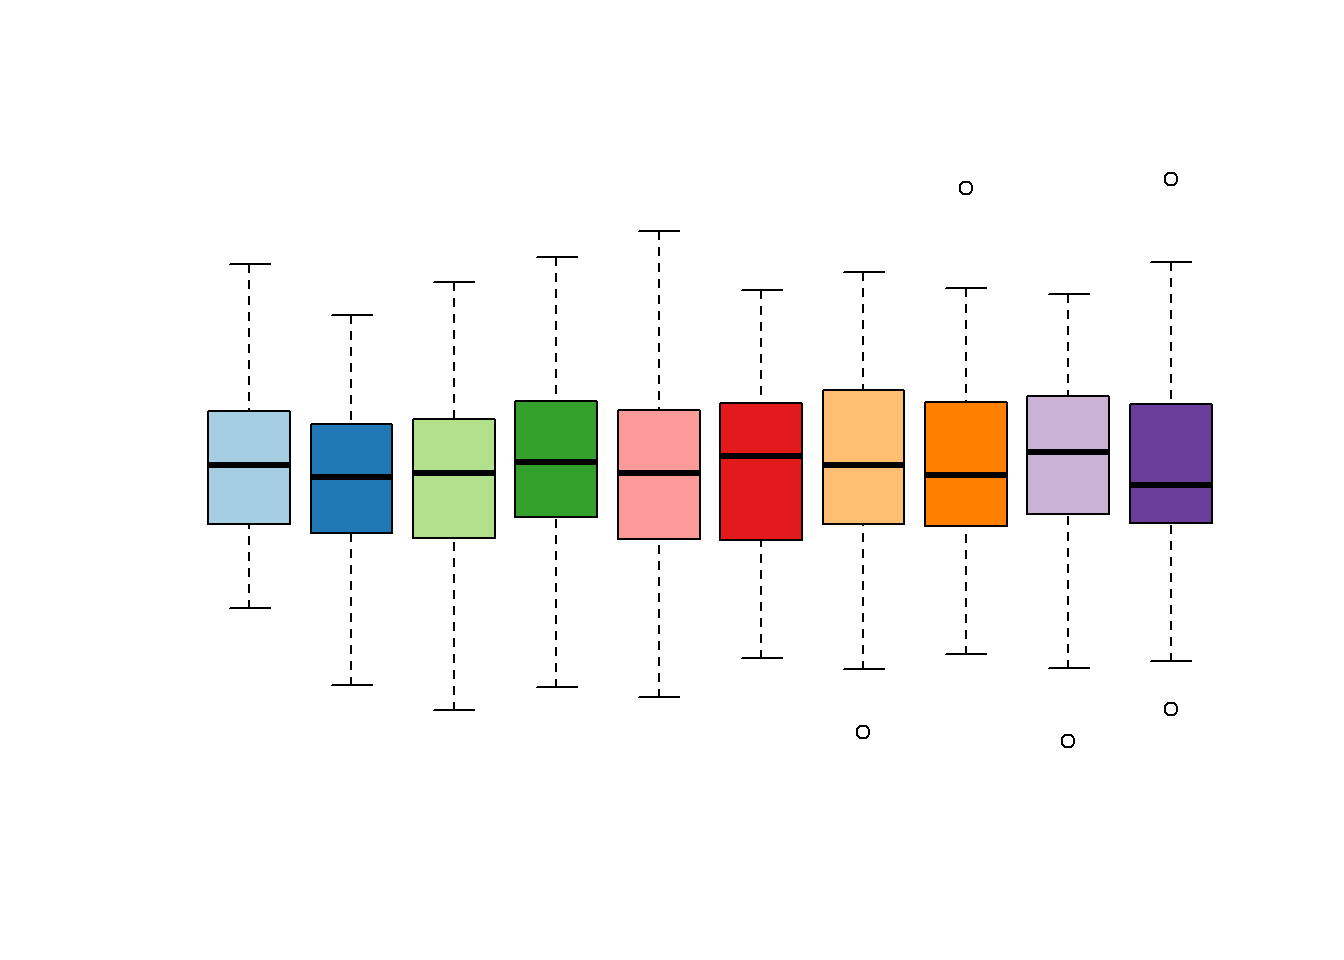
\includegraphics{myRBook_FR_files/figure-latex/unnamed-chunk-252-2.pdf}

\hypertarget{palettesforr}{%
\subsection{\texorpdfstring{\texttt{palettesForR}}{palettesForR}}\label{palettesforr}}

Le package \texttt{palettesForR} est un autre package contenant des palettes prêtes à l'emploi, issues des projets `Gimp' et `Inkscape'. Comme pour \texttt{RColorBrewer}, il suffit d'appeler les palettes pour les utiliser. Les nombreuses palettes disponibles sont listées dans l'aide du package. Voici un exemple d'utilisation.

\begin{Shaded}
\begin{Highlighting}[]
\NormalTok{pkgCheck <-}\StringTok{ }\ControlFlowTok{function}\NormalTok{(x)\{ }
    \ControlFlowTok{if}\NormalTok{ (}\OperatorTok{!}\KeywordTok{require}\NormalTok{(x, }\DataTypeTok{character.only =} \OtherTok{TRUE}\NormalTok{))\{}
        \KeywordTok{install.packages}\NormalTok{(x, }\DataTypeTok{dependencies =} \OtherTok{TRUE}\NormalTok{)}
        \ControlFlowTok{if}\NormalTok{(}\OperatorTok{!}\KeywordTok{require}\NormalTok{(x, }\DataTypeTok{character.only =} \OtherTok{TRUE}\NormalTok{)) \{}
            \KeywordTok{stop}\NormalTok{()}
\NormalTok{        \}}
\NormalTok{    \}}
\NormalTok{\}}
\KeywordTok{pkgCheck}\NormalTok{(}\StringTok{"palettesForR"}\NormalTok{)}
\KeywordTok{showPalette}\NormalTok{(Echo_gpl)}
\end{Highlighting}
\end{Shaded}

\includegraphics{myRBook_FR_files/figure-latex/unnamed-chunk-253-1.pdf}

\begin{Shaded}
\begin{Highlighting}[]
\NormalTok{groupTest <-}\StringTok{ }\KeywordTok{sample}\NormalTok{(}\DecValTok{1}\OperatorTok{:}\DecValTok{3}\NormalTok{, }\DataTypeTok{size =} \DecValTok{100}\NormalTok{, }\DataTypeTok{replace =} \OtherTok{TRUE}\NormalTok{) }
\NormalTok{valueTest <-}\StringTok{ }\KeywordTok{sample}\NormalTok{(}\DecValTok{1}\OperatorTok{:}\DecValTok{7}\NormalTok{, }\DataTypeTok{size =} \DecValTok{100}\NormalTok{, }\DataTypeTok{replace =} \OtherTok{TRUE}\NormalTok{)}
\NormalTok{tableTest <-}\StringTok{ }\KeywordTok{table}\NormalTok{(groupTest, valueTest)}
\KeywordTok{barplot}\NormalTok{(tableTest, }
  \DataTypeTok{col =}\NormalTok{ Echo_gpl, }\DataTypeTok{axes =} \OtherTok{FALSE}\NormalTok{, }\DataTypeTok{beside =} \OtherTok{TRUE}\NormalTok{)}
\end{Highlighting}
\end{Shaded}

\includegraphics{myRBook_FR_files/figure-latex/unnamed-chunk-253-2.pdf}

\begin{Shaded}
\begin{Highlighting}[]
\NormalTok{groupTest <-}\StringTok{ }\KeywordTok{sample}\NormalTok{(}\DecValTok{1}\OperatorTok{:}\DecValTok{3}\NormalTok{, }\DataTypeTok{size =} \DecValTok{100}\NormalTok{, }\DataTypeTok{replace =} \OtherTok{TRUE}\NormalTok{) }
\NormalTok{valueTest <-}\StringTok{ }\KeywordTok{sample}\NormalTok{(}\DecValTok{1}\OperatorTok{:}\DecValTok{7}\NormalTok{, }\DataTypeTok{size =} \DecValTok{100}\NormalTok{, }\DataTypeTok{replace =} \OtherTok{TRUE}\NormalTok{)}
\NormalTok{tableTest <-}\StringTok{ }\KeywordTok{table}\NormalTok{(groupTest, valueTest)}
\KeywordTok{barplot}\NormalTok{(tableTest, }
  \DataTypeTok{col =}\NormalTok{ Tango_gpl, }\DataTypeTok{axes =} \OtherTok{FALSE}\NormalTok{, }\DataTypeTok{beside =} \OtherTok{TRUE}\NormalTok{)}
\end{Highlighting}
\end{Shaded}

\includegraphics{myRBook_FR_files/figure-latex/unnamed-chunk-253-3.pdf}

\hypertarget{les-autres-packages}{%
\subsection{Les autres packages}\label{les-autres-packages}}

Il existe de très nombreux packages contenant des palettes. Par exemple :

\begin{itemize}
\tightlist
\item
  \texttt{viridis} (\url{https://CRAN.R-project.org/package=viridis})
\item
  \texttt{jcolors} (\url{https://CRAN.R-project.org/package=jcolors})
\item
  \texttt{scico} (\url{https://CRAN.R-project.org/package=scico})
\item
  \ldots{}
\end{itemize}

\hypertarget{ggplot2-package}{%
\section{ggplot2 package}\label{ggplot2-package}}

Le package \texttt{ggplot2} est une alternative aux fonctions de base de R pour réaliser des graphiques. Il repose sur ``La Grammaire des Graphiques'' de Leland Wilkinson et permet de réaliser des graphiques sous forme de couches, avec en général un rendu esthétique supérieur aux graphiques réalisés avec les fonctions R de base. Est-ce qu'il faut pour autant oublier ce qui a été vu jusqu'à présent et se concentrer sur l'utilisation de \texttt{ggplot2} ? Heureusement que non ! Si pour explorer un jeu de données et en sortir les tendances principales \texttt{ggplot2} s'avère parfois plus puissant, nos graphiques ne viennent jamais seuls et sont accompagnés d'analyses statistiques rendant nécessaire un travail souvent poussé sur la gestion des données. Une fois nos hypothèses de travail testées statistiquement, il devient facile de réaliser nos graphiques quel que soit leur niveau de complexité (avec les fonctions de base ou avec \texttt{ggplot2}). Par ailleurs nous verrons dans le chapitre suivant que depuis le graphique jusqu'à la figure dans l'article scientifique, il y a une série de traitements à effectuer et la manipulation des paramètres esthétiques peut se faire indépendamment de R. Donc \texttt{ggplot2} est un package intéressant car il apporte une alternative avec une autre philosophie dans la construction des graphiques, mais il ne se substitue pas à ce que nous venons d'apprendre jusqu'à présent. Dans la pratique nous pourrons utiliser l'un ou l'autre en fonction des données et des manipulations que nous souhaitons en faire.

Pour revenir à \texttt{ggplot2}, commençons par un exemple avec les données \texttt{iris}.

\begin{Shaded}
\begin{Highlighting}[]
\NormalTok{pkgCheck <-}\StringTok{ }\ControlFlowTok{function}\NormalTok{(x)\{ }
    \ControlFlowTok{if}\NormalTok{ (}\OperatorTok{!}\KeywordTok{require}\NormalTok{(x, }\DataTypeTok{character.only =} \OtherTok{TRUE}\NormalTok{))\{}
        \KeywordTok{install.packages}\NormalTok{(x, }\DataTypeTok{dependencies =} \OtherTok{TRUE}\NormalTok{)}
        \ControlFlowTok{if}\NormalTok{(}\OperatorTok{!}\KeywordTok{require}\NormalTok{(x, }\DataTypeTok{character.only =} \OtherTok{TRUE}\NormalTok{)) \{}
            \KeywordTok{stop}\NormalTok{()}
\NormalTok{        \}}
\NormalTok{    \}}
\NormalTok{\}}
\KeywordTok{pkgCheck}\NormalTok{(}\StringTok{"ggplot2"}\NormalTok{)}
\KeywordTok{data}\NormalTok{(iris)}
\CommentTok{# ggplot2}
\NormalTok{p <-}\StringTok{ }\KeywordTok{ggplot}\NormalTok{(}\DataTypeTok{data =}\NormalTok{ iris, }\KeywordTok{aes}\NormalTok{(}\DataTypeTok{x =}\NormalTok{ Sepal.Length, }\DataTypeTok{y =}\NormalTok{ Sepal.Width))}
\NormalTok{p }\OperatorTok{+}\StringTok{ }\KeywordTok{geom_point}\NormalTok{() }\OperatorTok{+}\StringTok{ }\KeywordTok{ggtitle}\NormalTok{(}\StringTok{"ggplot2"}\NormalTok{)}
\end{Highlighting}
\end{Shaded}

\includegraphics{myRBook_FR_files/figure-latex/unnamed-chunk-254-1.pdf}

\begin{Shaded}
\begin{Highlighting}[]
\CommentTok{# base}
\KeywordTok{plot}\NormalTok{(}\DataTypeTok{x =}\NormalTok{ iris}\OperatorTok{$}\NormalTok{Sepal.Length, }\DataTypeTok{y =}\NormalTok{ iris}\OperatorTok{$}\NormalTok{Sepal.Width, }
  \DataTypeTok{main =} \StringTok{"base"}\NormalTok{, }\DataTypeTok{pch =} \DecValTok{16}\NormalTok{)}
\end{Highlighting}
\end{Shaded}

\includegraphics{myRBook_FR_files/figure-latex/unnamed-chunk-254-2.pdf}

Maintenant séparons l'information en fonction de l'espèce de fleur.

\begin{Shaded}
\begin{Highlighting}[]
\CommentTok{# ggplot2}
\NormalTok{p <-}\StringTok{ }\KeywordTok{ggplot}\NormalTok{(}\DataTypeTok{data =}\NormalTok{ iris, }\KeywordTok{aes}\NormalTok{(}\DataTypeTok{x =}\NormalTok{ Sepal.Length, }\DataTypeTok{y =}\NormalTok{ Sepal.Width, }\DataTypeTok{colour =}\NormalTok{ Species))}
\NormalTok{p }\OperatorTok{+}\StringTok{ }\KeywordTok{geom_point}\NormalTok{() }\OperatorTok{+}\StringTok{ }\KeywordTok{ggtitle}\NormalTok{(}\StringTok{"ggplot2"}\NormalTok{)}
\end{Highlighting}
\end{Shaded}

\includegraphics{myRBook_FR_files/figure-latex/unnamed-chunk-255-1.pdf}

\begin{Shaded}
\begin{Highlighting}[]
\CommentTok{# base}
\KeywordTok{plot}\NormalTok{(}\DataTypeTok{x =}\NormalTok{ iris}\OperatorTok{$}\NormalTok{Sepal.Length, }\DataTypeTok{y =}\NormalTok{ iris}\OperatorTok{$}\NormalTok{Sepal.Width, }
  \DataTypeTok{main =} \StringTok{"base"}\NormalTok{, }\DataTypeTok{pch =} \DecValTok{16}\NormalTok{, }\DataTypeTok{col =}\NormalTok{ iris}\OperatorTok{$}\NormalTok{Species)}
\end{Highlighting}
\end{Shaded}

\includegraphics{myRBook_FR_files/figure-latex/unnamed-chunk-255-2.pdf}

Il semble y avoir une relation entre largeur et longueur des sépales par espèces.

\begin{Shaded}
\begin{Highlighting}[]
\CommentTok{# linear regressions}
\NormalTok{lmFits <-}\StringTok{ }\KeywordTok{lapply}\NormalTok{(}\DecValTok{1}\OperatorTok{:}\DecValTok{3}\NormalTok{, }\ControlFlowTok{function}\NormalTok{(i)\{}
\NormalTok{  fitSp1 <-}\StringTok{ }\KeywordTok{lm}\NormalTok{(iris}\OperatorTok{$}\NormalTok{Sepal.Width[}\KeywordTok{as.numeric}\NormalTok{(iris}\OperatorTok{$}\NormalTok{Species) }\OperatorTok{==}\StringTok{ }\NormalTok{i] }\OperatorTok{~}\StringTok{ }
\StringTok{    }\NormalTok{iris}\OperatorTok{$}\NormalTok{Sepal.Length[}\KeywordTok{as.numeric}\NormalTok{(iris}\OperatorTok{$}\NormalTok{Species) }\OperatorTok{==}\StringTok{ }\NormalTok{i])}
\NormalTok{  fStat1 <-}\StringTok{ }\KeywordTok{summary}\NormalTok{(fitSp1)}\OperatorTok{$}\NormalTok{fstatistic}
\NormalTok{  rSq1 <-}\StringTok{ }\KeywordTok{summary}\NormalTok{(fitSp1)}\OperatorTok{$}\NormalTok{r.squared}
\NormalTok{  pVal1 <-}\StringTok{ }\KeywordTok{summary}\NormalTok{(fitSp1)}\OperatorTok{$}\NormalTok{coefficients[}\DecValTok{2}\NormalTok{, }\DecValTok{4}\NormalTok{]}
\NormalTok{  stat1 <-}\StringTok{ }\KeywordTok{paste0}\NormalTok{(}\StringTok{"F="}\NormalTok{, }\KeywordTok{round}\NormalTok{(fStat1[}\DecValTok{1}\NormalTok{], }\DataTypeTok{digits =} \DecValTok{2}\NormalTok{), }
    \StringTok{"; DF="}\NormalTok{, fStat1[}\DecValTok{2}\NormalTok{], }\StringTok{"/"}\NormalTok{, fStat1[}\DecValTok{3}\NormalTok{], }\StringTok{"; r-sq="}\NormalTok{, }\KeywordTok{round}\NormalTok{(rSq1, }\DataTypeTok{digits =} \DecValTok{2}\NormalTok{), }
    \StringTok{"; p-val="}\NormalTok{, }\KeywordTok{round}\NormalTok{(pVal1, }\DataTypeTok{digits =} \DecValTok{6}\NormalTok{))}
  \KeywordTok{return}\NormalTok{(}\KeywordTok{list}\NormalTok{(fitSp1, stat1))}
\NormalTok{\})}
\CommentTok{# ggplot2}
\NormalTok{p <-}\StringTok{ }\KeywordTok{ggplot}\NormalTok{(}\DataTypeTok{data =}\NormalTok{ iris, }\KeywordTok{aes}\NormalTok{(}\DataTypeTok{x =}\NormalTok{ Sepal.Length, }\DataTypeTok{y =}\NormalTok{ Sepal.Width, }\DataTypeTok{colour =}\NormalTok{ Species))}
\NormalTok{p <-}\StringTok{ }\NormalTok{p }\OperatorTok{+}\StringTok{ }\KeywordTok{geom_point}\NormalTok{() }\OperatorTok{+}\StringTok{ }\KeywordTok{ggtitle}\NormalTok{(}\StringTok{"ggplot2"}\NormalTok{) }\OperatorTok{+}\StringTok{ }\KeywordTok{stat_smooth}\NormalTok{(}\DataTypeTok{method =} \StringTok{"lm"}\NormalTok{, }\DataTypeTok{se =} \OtherTok{FALSE}\NormalTok{)}
\NormalTok{p <-}\StringTok{ }\NormalTok{p }\OperatorTok{+}\StringTok{ }\KeywordTok{annotate}\NormalTok{(}\DataTypeTok{geom =} \StringTok{"text"}\NormalTok{, }\DataTypeTok{x =} \DecValTok{6}\NormalTok{, }\DataTypeTok{y =} \FloatTok{2.250}\NormalTok{, }\DataTypeTok{label =}\NormalTok{ lmFits[[}\DecValTok{1}\NormalTok{]][[}\DecValTok{2}\NormalTok{]], }\DataTypeTok{colour =} \DecValTok{2}\NormalTok{)}
\NormalTok{p <-}\StringTok{ }\NormalTok{p }\OperatorTok{+}\StringTok{ }\KeywordTok{annotate}\NormalTok{(}\DataTypeTok{geom =} \StringTok{"text"}\NormalTok{, }\DataTypeTok{x =} \DecValTok{6}\NormalTok{, }\DataTypeTok{y =} \FloatTok{2.125}\NormalTok{, }\DataTypeTok{label =}\NormalTok{ lmFits[[}\DecValTok{2}\NormalTok{]][[}\DecValTok{2}\NormalTok{]], }\DataTypeTok{colour =} \DecValTok{3}\NormalTok{)}
\NormalTok{p <-}\StringTok{ }\NormalTok{p }\OperatorTok{+}\StringTok{ }\KeywordTok{annotate}\NormalTok{(}\DataTypeTok{geom =} \StringTok{"text"}\NormalTok{, }\DataTypeTok{x =} \DecValTok{6}\NormalTok{, }\DataTypeTok{y =} \FloatTok{2.000}\NormalTok{, }\DataTypeTok{label =}\NormalTok{ lmFits[[}\DecValTok{3}\NormalTok{]][[}\DecValTok{2}\NormalTok{]], }\DataTypeTok{colour =} \DecValTok{4}\NormalTok{)}
\NormalTok{p}
\end{Highlighting}
\end{Shaded}

\includegraphics{myRBook_FR_files/figure-latex/unnamed-chunk-256-1.pdf}

\begin{Shaded}
\begin{Highlighting}[]
\CommentTok{# base}
\KeywordTok{plot}\NormalTok{(}\DataTypeTok{x =}\NormalTok{ iris}\OperatorTok{$}\NormalTok{Sepal.Length, }\DataTypeTok{y =}\NormalTok{ iris}\OperatorTok{$}\NormalTok{Sepal.Width, }
  \DataTypeTok{main =} \StringTok{"base"}\NormalTok{, }\DataTypeTok{pch =} \DecValTok{16}\NormalTok{, }\DataTypeTok{col =}\NormalTok{ iris}\OperatorTok{$}\NormalTok{Species)}
\KeywordTok{abline}\NormalTok{(lmFits[[}\DecValTok{1}\NormalTok{]][[}\DecValTok{1}\NormalTok{]], }\DataTypeTok{col =} \DecValTok{1}\NormalTok{)}
\KeywordTok{abline}\NormalTok{(lmFits[[}\DecValTok{2}\NormalTok{]][[}\DecValTok{1}\NormalTok{]], }\DataTypeTok{col =} \DecValTok{2}\NormalTok{)}
\KeywordTok{abline}\NormalTok{(lmFits[[}\DecValTok{3}\NormalTok{]][[}\DecValTok{1}\NormalTok{]], }\DataTypeTok{col =} \DecValTok{3}\NormalTok{)}
\KeywordTok{text}\NormalTok{(}\DataTypeTok{x =} \FloatTok{5.5}\NormalTok{, }\DataTypeTok{y =} \FloatTok{2.2}\NormalTok{, }\DataTypeTok{labels =}\NormalTok{ lmFits[[}\DecValTok{1}\NormalTok{]][[}\DecValTok{2}\NormalTok{]], }\DataTypeTok{pos =} \DecValTok{4}\NormalTok{)}
\KeywordTok{text}\NormalTok{(}\DataTypeTok{x =} \FloatTok{5.5}\NormalTok{, }\DataTypeTok{y =} \FloatTok{2.1}\NormalTok{, }\DataTypeTok{labels =}\NormalTok{ lmFits[[}\DecValTok{2}\NormalTok{]][[}\DecValTok{2}\NormalTok{]], }\DataTypeTok{pos =} \DecValTok{4}\NormalTok{, }\DataTypeTok{col =} \DecValTok{2}\NormalTok{)}
\KeywordTok{text}\NormalTok{(}\DataTypeTok{x =} \FloatTok{5.5}\NormalTok{, }\DataTypeTok{y =} \FloatTok{2.0}\NormalTok{, }\DataTypeTok{labels =}\NormalTok{ lmFits[[}\DecValTok{3}\NormalTok{]][[}\DecValTok{2}\NormalTok{]], }\DataTypeTok{pos =} \DecValTok{4}\NormalTok{, }\DataTypeTok{col =} \DecValTok{3}\NormalTok{)}
\end{Highlighting}
\end{Shaded}

\includegraphics{myRBook_FR_files/figure-latex/unnamed-chunk-256-2.pdf}

Nous pouvons voir sur ces exemples que les graphiques avec \texttt{ggplot2} commencent par un appel de la fonction \texttt{ggplot()}, dans laquelle le premier argument \texttt{data} correspond à nos données (typiquement une \texttt{data.frame}), et le deuxième argument \texttt{aes()} correspond aux informations que nous souhaitons utiliser. Par convention cette information est stockée dans un objet \texttt{p}. Nous allons ensuite ajouter des couches supplémentaires en utilisant \texttt{+}.

Dans les couches nous pouvons ajouter des aspects géométriques (le type de graphique, par exemple \texttt{geom\_point()}), des statistiques (par exemple \texttt{stat\_smooth()}), des annotations (par exemple \texttt{annotate()}), et bien d'autres choses liées aux axes, aux couleurs, \ldots{} La documentation complète (en anglais) peut être consultée à l'adresse \url{https://ggplot2.tidyverse.org/} (fiche de résumé : \url{https://github.com/rstudio/cheatsheets/blob/master/data-visualization-2.1.pdf}). De nombreuses extensions à \texttt{ggplot2} sont disponibles à l'adresse \url{http://www.ggplot2-exts.org/gallery/}.

\hypertarget{les-graphiques-interactifs-et-dynamiques-avec-plotly}{%
\section{\texorpdfstring{Les graphiques interactifs et dynamiques avec \texttt{Plotly}}{Les graphiques interactifs et dynamiques avec Plotly}}\label{les-graphiques-interactifs-et-dynamiques-avec-plotly}}

\texttt{Plotly} est un package permettant de réaliser des graphiques interactifs et dynamiques. Cela peut être particulièrement utile pour les résultats ayant vocation à être diffusées sur Internet. Le package s'installe comme tous les autres avec \texttt{install.packages("plotly")}. Le package est gratuit et open source.

Cet exemple a été copié depuis le livre de Carson Sievert (\url{https://plotly-book.cpsievert.me}). Le code qui a permis de faire ce graphique est sous licence Creative Commons Attribution-NonCommercial-NoDerivs 3.0 United States License (Carson Sievert ; \url{https://creativecommons.org/licenses/by-nc-nd/3.0/us/}).

\includegraphics{myRBook_FR_files/figure-latex/unnamed-chunk-257-1.pdf}

\hypertarget{conclusion-10}{%
\section{Conclusion}\label{conclusion-10}}

Ce chapitre nous a permis de survoler d'autres options graphiques et en particulier les packages \texttt{ggplot2} et \texttt{plotly}. Des livres spécifiques (en anglais) couvrent tous les aspects de ces packages, ici l'objectif est de savoir que ces options existent pour y avoir recours si besoin. Les sites web ``Data to Viz'' et ``r-graph gallery'' (\url{https://www.data-to-viz.com} ; \url{https://www.r-graph-gallery.com/}) permettront de se faire une idée des possibilités offertes par R quant aux représentations graphiques. Le chapitre suivant traite des processus nécessaires pour transformer un graphique R en une figure publiable dans un article scientifique. A très bientôt !

\hypertarget{graph4}{%
\chapter{Du graphique à la figure dans un article scientifique}\label{graph4}}

Une fois nos résultats obtenus, il est primordial de les publier. Ce n'est qu'en publiant nos résultats que nous participons à la science. Cela peut se faire via des communications dans des congrès, via des posters, ou encore (et c'est le plus fréquent), via des articles scientifiques.

Dans les articles scientifiques, les résultats graphiques prennent la forme de \emph{figures} qui sont souvent le fruit de un ou plusieurs graphiques. Ces figures suivent des critères bien précis dictés par la revue. Prenons cet exemple adapté et traduit du guide de la revue PLoS :

\emph{Les fichiers doivent être au format TIFF (avec compression LZW et une seule couche), ou EPS. Les dimensions doivent être de 789 à 2250 pixels et une hauteur maximum de 2625 pixels pour une résolution de 300 dpi (entre 6.68 et 19.05 cm de large - maximum 13.2 cm pour un alignement sur une colonne - et maximum 22.23 cm de haut). La police doit être Arial, Times, ou Symbol et d'une taille entre 8 et 12 points.}

Il est difficile de respecter toutes ces contraintes avec R. C'est pourquoi nous allons utiliser des logiciels tiers pour transformer nos graphiques en figures. Nous allons utiliser Inkscape pour la mise en page et Gimp pour la transformation dans les formats requis.

Quant on prend une photo, chaque pixel prend une valeur qui va définir la couleur du pixel, donc en zoomant sur une photo on va voir apparaître les pixels (nous perdons en netteté). C'est une image \emph{matricielle}. Dans une image \emph{vectorielle}, les éléments sont codés sous forme de segments, nous ne perdons pas en qualité car chaque élément conserve ses coordonées (Figure \ref{fig:matVec}). L'avantage des images vectorielles est que l'on peut modifier les éléments de l'image sans perdre en qualité. C'est ce que nous allons faire avec Inkscape. L'avantage des images matricielles est que l'on peut choisir entre de très nombreux formats (dont TIFF). C'est ce que nous allons faire avec Gimp.

\begin{figure}
\includegraphics[width=4.85in]{myFigures/matVec} \caption{Image matricielle et vectorielle.\label{fig:matVec}}\label{fig:matVec}
\end{figure}

\hypertarget{inkscape}{%
\section{Inkscape}\label{inkscape}}

\begin{figure}
\includegraphics[width=4.17in]{myLogos/logoInkscape} \caption{Logo Inkscape (https://inkscape.org).\label{fig:logoInkscape}}\label{fig:logoInkscape}
\end{figure}

Inkscape est un logiciel de dessin vectoriel disponible sous Windows, Mac OS X et GNU/Linux. C'est un logiciel libre et open source sous licence GPL. Nous pouvons le télécharger à l'adresse suivante \url{https://inkscape.org}. Inksacpe est déjà installé par défaut sur de nombreuses distributions de Linux.

XXX

\hypertarget{the-gimp}{%
\section{The Gimp}\label{the-gimp}}

\begin{figure}
\includegraphics[width=4.17in]{myLogos/logoGimp} \caption{Logo Gimp (https://www.gimp.org/).\label{fig:logoGimp}}\label{fig:logoGimp}
\end{figure}

Gimp est un logiciel de dessin matriciel disponible sous Windows, Mac OS X et GNU/Linux. C'est un logiciel libre et open source sous licence GPL. Nous pouvons le télécharger à l'adresse suivante \url{https://www.gimp.org/}. Gimp signifie ``GNU Image Manipulation Program''. Gimp est déjà installé par défaut sur de nombreuses distributions de Linux.

XXX

\hypertarget{table-de-reference}{%
\section{Table de référence}\label{table-de-reference}}

XXX \ref{tab:tabRefPub}

\begin{table}[t]

\caption{\label{tab:tabRefPub}Table de référence pour la construction des figures.\label{tab:tabRefPub}}
\centering
\begin{tabular}{l|l|l|l|l|l|l}
\hline
Revue & Largeur & Hauteur & Format & Resolution & Police & Taille\\
\hline
PLoS & 6.68-19.05 & max 22.23 & TIFF, EPS & 300-600 dpi & Arial, Times, Symbol & 9-12\\
\hline
PNAS & 8.7; 11.4; 17.8 & max 22.5 & TIF, EPS & 300 dpi & Arial, Helvetica, Times, Symbol, Mathematical Pi, European Pi & min 6-8\\
\hline
Science & 9; 12.7; 18.4 & NA & AI, EPS, PDF, TIF, JPEG & 300 dpi & Helvetica & panel 10, axis 6-9, font 5\\
\hline
\end{tabular}
\end{table}

\hypertarget{part-etude-de-cas}{%
\part{Etude de cas}\label{part-etude-de-cas}}

\hypertarget{studyCase001}{%
\chapter{Analyser des données de datalogger de température}\label{studyCase001}}

Dans les études de biologie, d'écologie ou d'agronomie, nous utilisons fréquemment des données de température provenant de dataloggers. Dans cette étude de cas, nous verrons comment analyser ces données en utilisant les données de température de l'altiplano bolivien près de la ville de El Alto. La première étape consiste à transformer les données du datalogger en un format facile à lire pour R. Nous utiliserons un fichier CSV et la fonction \protect\hyperlink{import}{\texttt{read.table()}}. Le fichier peut être téléchargé à partir du site Web du livre sur GitHub (\url{https://github.com/frareb/myRBook_FR/blob/master/myFiles/E05C13.csv}), ou alors lu directement par R depuis sa source (\url{https://raw.githubusercontent.com/frareb/myRBook_FR/master/myFiles/E05C13.csv}).

\begin{Shaded}
\begin{Highlighting}[]
\CommentTok{# Lecture du fichier en local après téléchargement : }
\NormalTok{bdd <-}\StringTok{ }\KeywordTok{read.table}\NormalTok{(}\StringTok{"myFiles/E05C13.csv"}\NormalTok{, }\DataTypeTok{skip =} \DecValTok{1}\NormalTok{, }\DataTypeTok{header =} \OtherTok{TRUE}\NormalTok{, }
  \DataTypeTok{sep =} \StringTok{","}\NormalTok{, }\DataTypeTok{dec =} \StringTok{"."}\NormalTok{, }\DataTypeTok{stringsAsFactors =} \OtherTok{FALSE}\NormalTok{)}
\CommentTok{# Lecture du fichier depuis GitHub : }
\CommentTok{# bdd <- read.table("https://raw.githubusercontent.com/frareb/myRBook_FR/master/myFiles/E05C13.csv", }
\CommentTok{#   skip = 1, header = TRUE, sep = ",", dec = ".", stringsAsFactors = FALSE)}
\KeywordTok{colnames}\NormalTok{(bdd) <-}\StringTok{ }\KeywordTok{c}\NormalTok{(}\StringTok{"id"}\NormalTok{, }\StringTok{"date"}\NormalTok{, }\StringTok{"temp"}\NormalTok{)}
\KeywordTok{head}\NormalTok{(bdd)}
\end{Highlighting}
\end{Shaded}

\begin{verbatim}
##   id              date  temp
## 1  1 11/12/15 23:00:00 4.973
## 2  2 11/12/15 23:30:00 4.766
## 3  3 11/13/15 00:00:00 4.844
## 4  4 11/13/15 00:30:00 4.844
## 5  5 11/13/15 01:00:00 5.076
## 6  6 11/13/15 01:30:00 5.282
\end{verbatim}

\begin{Shaded}
\begin{Highlighting}[]
\KeywordTok{tail}\NormalTok{(bdd)}
\end{Highlighting}
\end{Shaded}

\begin{verbatim}
##          id              date  temp
## 32781 32781 09/25/17 21:00:00 7.091
## 32782 32782 09/25/17 21:30:00 6.914
## 32783 32783 09/25/17 22:00:00 6.813
## 32784 32784 09/25/17 22:30:00 6.611
## 32785 32785 09/25/17 23:00:00 6.331
## 32786 32786 09/25/17 23:30:00 5.385
\end{verbatim}

\begin{Shaded}
\begin{Highlighting}[]
\KeywordTok{str}\NormalTok{(bdd)}
\end{Highlighting}
\end{Shaded}

\begin{verbatim}
## 'data.frame':    32786 obs. of  3 variables:
##  $ id  : int  1 2 3 4 5 6 7 8 9 10 ...
##  $ date: chr  "11/12/15 23:00:00" "11/12/15 23:30:00" "11/13/15 00:00:00" "11/13/15 00:30:00" ...
##  $ temp: num  4.97 4.77 4.84 4.84 5.08 ...
\end{verbatim}

Nous pouvons voir que la date est au format \texttt{character} et qu'elle contient la date avec le mois, le jour et l'année séparés par \texttt{/}, puis vient un espace et l'heure avec des heures de 0 à 24, minutes et secondes, séparés par \texttt{:} (exemple: \texttt{11/12/15\ 23:00:00} pour le 12 novembre 2015 à 11 heures du soir). Nous allons séparer les informations en plusieurs objets. Séparons d'abord la date de l'heure. Pour cela, nous utiliserons la fonction \texttt{strsplit()} en utilisant l'espace entre la date et l'heure comme séparateur.

\begin{Shaded}
\begin{Highlighting}[]
\KeywordTok{strsplit}\NormalTok{(}\StringTok{"11/12/15 23:00:00"}\NormalTok{, }\DataTypeTok{split =} \StringTok{" "}\NormalTok{)}
\end{Highlighting}
\end{Shaded}

\begin{verbatim}
## [[1]]
## [1] "11/12/15" "23:00:00"
\end{verbatim}

Comme l'indiquent les doubles crochets, la fonction \texttt{strsplit()} renvoie un objet au format \texttt{list}. Nous voulons le vecteur qui correspond au premier élément de la liste, donc nous allons ajouter \texttt{{[}{[}1{]}{]}}.

\begin{Shaded}
\begin{Highlighting}[]
\KeywordTok{strsplit}\NormalTok{(}\StringTok{"11/12/15 23:00:00"}\NormalTok{, }\DataTypeTok{split =} \StringTok{" "}\NormalTok{)[[}\DecValTok{1}\NormalTok{]]}
\end{Highlighting}
\end{Shaded}

\begin{verbatim}
## [1] "11/12/15" "23:00:00"
\end{verbatim}

Le premier élément du \texttt{vector} est la date. Pour avoir toutes les dates, nous allons faire une boucle avec la fonction \texttt{sapply()}.

\begin{Shaded}
\begin{Highlighting}[]
\NormalTok{bddDay <-}\StringTok{ }\KeywordTok{sapply}\NormalTok{(}\KeywordTok{strsplit}\NormalTok{(bdd[, }\DecValTok{2}\NormalTok{], }\DataTypeTok{split =} \StringTok{" "}\NormalTok{), }\StringTok{"[["}\NormalTok{, }\DecValTok{1}\NormalTok{)}
\KeywordTok{head}\NormalTok{(bddDay)}
\end{Highlighting}
\end{Shaded}

\begin{verbatim}
## [1] "11/12/15" "11/12/15" "11/13/15" "11/13/15" "11/13/15" "11/13/15"
\end{verbatim}

Ensuite, nous aurons besoin des dates dans le format \texttt{Date}. pour cela nous allons transformer l'objet au format \texttt{Date} avec la fonction \texttt{as.Date()}.

\begin{Shaded}
\begin{Highlighting}[]
\NormalTok{bddDay <-}\StringTok{ }\KeywordTok{as.Date}\NormalTok{(}\KeywordTok{sapply}\NormalTok{(}\KeywordTok{strsplit}\NormalTok{(bdd[, }\DecValTok{2}\NormalTok{], }\DataTypeTok{split =} \StringTok{" "}\NormalTok{), }\StringTok{"[["}\NormalTok{, }\DecValTok{1}\NormalTok{), }\DataTypeTok{format =} \StringTok{"%m/%d/%y"}\NormalTok{)}
\KeywordTok{head}\NormalTok{(bddDay)}
\end{Highlighting}
\end{Shaded}

\begin{verbatim}
## [1] "2015-11-12" "2015-11-12" "2015-11-13" "2015-11-13" "2015-11-13"
## [6] "2015-11-13"
\end{verbatim}

Nous allons maintenant ajouter l'objet \texttt{bddDay} à notre \texttt{data.frame} \texttt{bdd}. Ensuite, nous allons vérifier que cette nouvelle colonne dans notre \texttt{data.frame} est bien au format \texttt{Date} avec la fonction \texttt{str()}

\begin{Shaded}
\begin{Highlighting}[]
\NormalTok{bdd}\OperatorTok{$}\NormalTok{day <-}\StringTok{ }\NormalTok{bddDay}
\KeywordTok{str}\NormalTok{(bdd)}
\end{Highlighting}
\end{Shaded}

\begin{verbatim}
## 'data.frame':    32786 obs. of  4 variables:
##  $ id  : int  1 2 3 4 5 6 7 8 9 10 ...
##  $ date: chr  "11/12/15 23:00:00" "11/12/15 23:30:00" "11/13/15 00:00:00" "11/13/15 00:30:00" ...
##  $ temp: num  4.97 4.77 4.84 4.84 5.08 ...
##  $ day : Date, format: "2015-11-12" "2015-11-12" ...
\end{verbatim}

Si l'information concernant la date n'est pas suffisante, nous pouvons ajouter l'heure. Dans ce cas c'est le format \texttt{POSIX} qu'il faudra utiliser avec la fonction \texttt{as.POSIXct()}. De la même manière nous allons ajouter l'information dans notre objet \texttt{bdd} et vérifier le format avec la fonction \texttt{str()}.

\begin{Shaded}
\begin{Highlighting}[]
\NormalTok{bddPosix <-}\StringTok{ }\KeywordTok{as.POSIXct}\NormalTok{(bdd}\OperatorTok{$}\NormalTok{date, }\DataTypeTok{format =} \StringTok{"%m/%d/%y %H:%M:%S"}\NormalTok{)}
\KeywordTok{head}\NormalTok{(bddPosix)}
\end{Highlighting}
\end{Shaded}

\begin{verbatim}
## [1] "2015-11-12 23:00:00 CET" "2015-11-12 23:30:00 CET"
## [3] "2015-11-13 00:00:00 CET" "2015-11-13 00:30:00 CET"
## [5] "2015-11-13 01:00:00 CET" "2015-11-13 01:30:00 CET"
\end{verbatim}

\begin{Shaded}
\begin{Highlighting}[]
\NormalTok{bdd}\OperatorTok{$}\NormalTok{posix <-}\StringTok{ }\NormalTok{bddPosix}
\KeywordTok{str}\NormalTok{(bdd)}
\end{Highlighting}
\end{Shaded}

\begin{verbatim}
## 'data.frame':    32786 obs. of  5 variables:
##  $ id   : int  1 2 3 4 5 6 7 8 9 10 ...
##  $ date : chr  "11/12/15 23:00:00" "11/12/15 23:30:00" "11/13/15 00:00:00" "11/13/15 00:30:00" ...
##  $ temp : num  4.97 4.77 4.84 4.84 5.08 ...
##  $ day  : Date, format: "2015-11-12" "2015-11-12" ...
##  $ posix: POSIXct, format: "2015-11-12 23:00:00" "2015-11-12 23:30:00" ...
\end{verbatim}

Dans les fonctions \texttt{as.Date()} et \texttt{as.POSIXct()}, nous avons utilisé l'argument \texttt{format} qui correspond au format dans lequel l'information sur la date est codée. Voici les éléments les plus courants pour le formatage de la date :

\begin{longtable}[]{@{}ll@{}}
\toprule
code & Valeur\tabularnewline
\midrule
\endhead
\%a & jour de la semaine (abréviation)\tabularnewline
\%A & jour de la semaine\tabularnewline
\%b & mois (abréviation)\tabularnewline
\%B & mois\tabularnewline
\%d & jour du mois (decimal)\tabularnewline
\%j & jour de l'année (decimal)\tabularnewline
\%m & mois (decimal)\tabularnewline
\%y & année avec deux chiffres\tabularnewline
\%Y & année\tabularnewline
\%U & semaine de l'année en commençant par dimanche (decimal)\tabularnewline
\%W & semaine de l'année en commençant par lundi (decimal)\tabularnewline
\%H & heure 24\tabularnewline
\%I & heure 12\tabularnewline
\%M & minute\tabularnewline
\%S & seconde\tabularnewline
\bottomrule
\end{longtable}

Nous pouvons visualiser les données avec la fonction \texttt{plot()}.

\begin{Shaded}
\begin{Highlighting}[]
\KeywordTok{plot}\NormalTok{(}\DataTypeTok{x =}\NormalTok{ bdd}\OperatorTok{$}\NormalTok{day, }\DataTypeTok{y =}\NormalTok{ bdd}\OperatorTok{$}\NormalTok{temp, }
    \DataTypeTok{type =} \StringTok{'l'}\NormalTok{, }\DataTypeTok{ylim =} \KeywordTok{c}\NormalTok{(}\OperatorTok{-}\DecValTok{15}\NormalTok{, }\DecValTok{40}\NormalTok{), }
    \DataTypeTok{xlab =} \StringTok{"Temps"}\NormalTok{, }\DataTypeTok{ylab =} \StringTok{"Température (°C)"}\NormalTok{)}
\end{Highlighting}
\end{Shaded}

\includegraphics{myRBook_FR_files/figure-latex/unnamed-chunk-265-1.pdf}

Nous pouvons simplifier les informations en ne calculant que les températures minimales, moyennes et maximales avec la fonction \texttt{tapply()}.

\begin{Shaded}
\begin{Highlighting}[]
\NormalTok{tempDayMean <-}\StringTok{ }\KeywordTok{tapply}\NormalTok{(bdd}\OperatorTok{$}\NormalTok{temp, }\DataTypeTok{INDEX =}\NormalTok{ bdd}\OperatorTok{$}\NormalTok{day, }\DataTypeTok{FUN =}\NormalTok{ mean)}
\NormalTok{tempDayMin <-}\StringTok{ }\KeywordTok{tapply}\NormalTok{(bdd}\OperatorTok{$}\NormalTok{temp, }\DataTypeTok{INDEX =}\NormalTok{ bdd}\OperatorTok{$}\NormalTok{day, }\DataTypeTok{FUN =}\NormalTok{ min)}
\NormalTok{tempDayMax <-}\StringTok{ }\KeywordTok{tapply}\NormalTok{(bdd}\OperatorTok{$}\NormalTok{temp, }\DataTypeTok{INDEX =}\NormalTok{ bdd}\OperatorTok{$}\NormalTok{day, }\DataTypeTok{FUN =}\NormalTok{ max)}
\KeywordTok{plot}\NormalTok{(}\DataTypeTok{x =} \KeywordTok{as.Date}\NormalTok{(}\KeywordTok{names}\NormalTok{(tempDayMean), }\DataTypeTok{format =} \StringTok{"%Y-%m-%d"}\NormalTok{), }
    \DataTypeTok{y =}\NormalTok{ tempDayMean, }\DataTypeTok{type =} \StringTok{'l'}\NormalTok{, }\DataTypeTok{ylim =} \KeywordTok{c}\NormalTok{(}\OperatorTok{-}\DecValTok{15}\NormalTok{, }\DecValTok{40}\NormalTok{), }
    \DataTypeTok{xlab =} \StringTok{"Temps"}\NormalTok{, }\DataTypeTok{ylab =} \StringTok{"Température (°C)"}\NormalTok{)}
\KeywordTok{points}\NormalTok{(}\KeywordTok{as.Date}\NormalTok{(}\KeywordTok{names}\NormalTok{(tempDayMin), }\DataTypeTok{format =} \StringTok{"%Y-%m-%d"}\NormalTok{), }
    \DataTypeTok{y =}\NormalTok{ tempDayMin, }\DataTypeTok{type =} \StringTok{'l'}\NormalTok{, }\DataTypeTok{col =} \DecValTok{4}\NormalTok{)}
\KeywordTok{points}\NormalTok{(}\KeywordTok{as.Date}\NormalTok{(}\KeywordTok{names}\NormalTok{(tempDayMax), }\DataTypeTok{format =} \StringTok{"%Y-%m-%d"}\NormalTok{), }
    \DataTypeTok{y =}\NormalTok{ tempDayMax, }\DataTypeTok{type =} \StringTok{'l'}\NormalTok{, }\DataTypeTok{col =} \DecValTok{2}\NormalTok{)}
\KeywordTok{legend}\NormalTok{(}\StringTok{"topright"}\NormalTok{, }\DataTypeTok{legend =} \KeywordTok{c}\NormalTok{(}\StringTok{"min"}\NormalTok{, }\StringTok{"max"}\NormalTok{, }\StringTok{"mean"}\NormalTok{), }
  \DataTypeTok{lty =} \DecValTok{1}\NormalTok{, }\DataTypeTok{lwd =} \DecValTok{2}\NormalTok{, }\DataTypeTok{col =} \KeywordTok{c}\NormalTok{(}\DecValTok{4}\NormalTok{, }\DecValTok{2}\NormalTok{, }\DecValTok{1}\NormalTok{))}
\end{Highlighting}
\end{Shaded}

\includegraphics{myRBook_FR_files/figure-latex/unnamed-chunk-266-1.pdf}

Nous pouvons très facilement représenter le même information par semaine. Il suffit de changer l'argument \texttt{INDEX} pour une date en semaine. Voici un exemple de format par semaine :

\begin{Shaded}
\begin{Highlighting}[]
\NormalTok{anoSem <-}\StringTok{ }\KeywordTok{format}\NormalTok{(bdd}\OperatorTok{$}\NormalTok{posix, }\DataTypeTok{format =} \StringTok{"%Y-%W"}\NormalTok{)}
\KeywordTok{head}\NormalTok{(anoSem)}
\end{Highlighting}
\end{Shaded}

\begin{verbatim}
## [1] "2015-45" "2015-45" "2015-45" "2015-45" "2015-45" "2015-45"
\end{verbatim}

Et voici le graphique par semaine :

\begin{Shaded}
\begin{Highlighting}[]
\NormalTok{tempWeekMean <-}\StringTok{ }\KeywordTok{tapply}\NormalTok{(bdd}\OperatorTok{$}\NormalTok{temp, }
  \DataTypeTok{INDEX =} \KeywordTok{format}\NormalTok{(bdd}\OperatorTok{$}\NormalTok{posix, }\DataTypeTok{format =} \StringTok{"%Y-%W-1"}\NormalTok{), }\DataTypeTok{FUN =}\NormalTok{ mean)}
\NormalTok{tempWeekMin <-}\StringTok{ }\KeywordTok{tapply}\NormalTok{(bdd}\OperatorTok{$}\NormalTok{temp, }
  \DataTypeTok{INDEX =} \KeywordTok{format}\NormalTok{(bdd}\OperatorTok{$}\NormalTok{posix, }\DataTypeTok{format =} \StringTok{"%Y-%W-1"}\NormalTok{), }\DataTypeTok{FUN =}\NormalTok{ min)}
\NormalTok{tempWeekMax <-}\StringTok{ }\KeywordTok{tapply}\NormalTok{(bdd}\OperatorTok{$}\NormalTok{temp, }
  \DataTypeTok{INDEX =} \KeywordTok{format}\NormalTok{(bdd}\OperatorTok{$}\NormalTok{posix, }\DataTypeTok{format =} \StringTok{"%Y-%W-1"}\NormalTok{), }\DataTypeTok{FUN =}\NormalTok{ max)}
\KeywordTok{plot}\NormalTok{(}\DataTypeTok{x =} \KeywordTok{as.Date}\NormalTok{(}\KeywordTok{names}\NormalTok{(tempWeekMean), }\DataTypeTok{format =} \StringTok{"%Y-%W-%u"}\NormalTok{), }
    \DataTypeTok{y =}\NormalTok{ tempWeekMean, }\DataTypeTok{type =} \StringTok{'l'}\NormalTok{, }\DataTypeTok{ylim =} \KeywordTok{c}\NormalTok{(}\OperatorTok{-}\DecValTok{15}\NormalTok{, }\DecValTok{40}\NormalTok{), }
    \DataTypeTok{xlab =} \StringTok{"Fecha"}\NormalTok{, }\DataTypeTok{ylab =} \StringTok{"Temperatura (°C)"}\NormalTok{)}
\KeywordTok{points}\NormalTok{(}\DataTypeTok{x =} \KeywordTok{as.Date}\NormalTok{(}\KeywordTok{names}\NormalTok{(tempWeekMin), }\DataTypeTok{format =} \StringTok{"%Y-%W-%u"}\NormalTok{), }
    \DataTypeTok{y =}\NormalTok{ tempWeekMin, }\DataTypeTok{type =} \StringTok{'l'}\NormalTok{, }\DataTypeTok{col =} \DecValTok{4}\NormalTok{)}
\KeywordTok{points}\NormalTok{(}\DataTypeTok{x =} \KeywordTok{as.Date}\NormalTok{(}\KeywordTok{names}\NormalTok{(tempWeekMax), }\DataTypeTok{format =} \StringTok{"%Y-%W-%u"}\NormalTok{), }
    \DataTypeTok{y =}\NormalTok{ tempWeekMax, }\DataTypeTok{type =} \StringTok{'l'}\NormalTok{, }\DataTypeTok{col =} \DecValTok{2}\NormalTok{)}
\KeywordTok{legend}\NormalTok{(}\StringTok{"topright"}\NormalTok{, }\DataTypeTok{legend =} \KeywordTok{c}\NormalTok{(}\StringTok{"min"}\NormalTok{, }\StringTok{"max"}\NormalTok{, }\StringTok{"promedio"}\NormalTok{), }
  \DataTypeTok{lty =} \DecValTok{1}\NormalTok{, }\DataTypeTok{lwd =} \DecValTok{2}\NormalTok{, }\DataTypeTok{col =} \KeywordTok{c}\NormalTok{(}\DecValTok{4}\NormalTok{, }\DecValTok{2}\NormalTok{, }\DecValTok{1}\NormalTok{))}
\end{Highlighting}
\end{Shaded}

\includegraphics{myRBook_FR_files/figure-latex/unnamed-chunk-268-1.pdf}

Dans ce type de représentation nous perdons l'information sur la variabilité des températures par semaine. En focntion des objectifs il pourra être intéressant de préférer une représentation sous forme de \texttt{boxplot} (ici un boxplot par mois en formattant la date avec \texttt{"\%Y-\%m"}).

\begin{Shaded}
\begin{Highlighting}[]
\KeywordTok{boxplot}\NormalTok{(bdd}\OperatorTok{$}\NormalTok{temp }\OperatorTok{~}\StringTok{ }\KeywordTok{format}\NormalTok{(bdd}\OperatorTok{$}\NormalTok{posix, }\DataTypeTok{format =} \StringTok{"%Y-%m"}\NormalTok{), }\DataTypeTok{las =} \DecValTok{3}\NormalTok{,}
  \DataTypeTok{xlab =} \StringTok{""}\NormalTok{, }\DataTypeTok{ylab =} \StringTok{"Température (°C)"}\NormalTok{)}
\end{Highlighting}
\end{Shaded}

\includegraphics{myRBook_FR_files/figure-latex/unnamed-chunk-269-1.pdf}

Pour comparer les différentes valeurs de température, il peut être utile d'attribuer une couleur à chaque boxplot. Par exemple, nous pouvons utiliser un gradient de couleur du bleu au rouge en utilisant la valeur de la température moyenne.

\begin{Shaded}
\begin{Highlighting}[]
\NormalTok{tempMonthMean <-}\StringTok{ }\KeywordTok{tapply}\NormalTok{(bdd}\OperatorTok{$}\NormalTok{temp, }
  \DataTypeTok{INDEX =} \KeywordTok{format}\NormalTok{(bdd}\OperatorTok{$}\NormalTok{posix, }\DataTypeTok{format =} \StringTok{"%Y-%m"}\NormalTok{), }\DataTypeTok{FUN =}\NormalTok{ mean)}
\NormalTok{myCol <-}\StringTok{ }\KeywordTok{colorRampPalette}\NormalTok{(}\KeywordTok{c}\NormalTok{(}\StringTok{"blue"}\NormalTok{, }\StringTok{"red"}\NormalTok{))(}\DecValTok{101}\NormalTok{)}
\NormalTok{tempMeanDayPos <-}\StringTok{ }\KeywordTok{round}\NormalTok{(}
\NormalTok{  (tempMonthMean }\OperatorTok{-}\StringTok{ }\KeywordTok{min}\NormalTok{(tempMonthMean)) }\OperatorTok{/}\StringTok{ }
\StringTok{    }\NormalTok{(}\KeywordTok{max}\NormalTok{(tempMonthMean) }\OperatorTok{-}\StringTok{ }\KeywordTok{min}\NormalTok{(tempMonthMean))}\OperatorTok{*}\DecValTok{100}\NormalTok{) }\OperatorTok{+}\StringTok{ }\DecValTok{1}
\KeywordTok{boxplot}\NormalTok{(bdd}\OperatorTok{$}\NormalTok{temp }\OperatorTok{~}\StringTok{ }\KeywordTok{format}\NormalTok{(bdd}\OperatorTok{$}\NormalTok{posix, }\DataTypeTok{format =} \StringTok{"%Y-%m"}\NormalTok{), }\DataTypeTok{las =} \DecValTok{3}\NormalTok{, }
  \DataTypeTok{col =}\NormalTok{ myCol[tempMeanDayPos],}
  \DataTypeTok{xlab =} \StringTok{""}\NormalTok{, }\DataTypeTok{ylab =} \StringTok{"Température (°C)"}\NormalTok{)}
\end{Highlighting}
\end{Shaded}

\includegraphics{myRBook_FR_files/figure-latex/unnamed-chunk-270-1.pdf}

Et pour celles et ceux qui utilisent \texttt{ggplot2} :

\begin{Shaded}
\begin{Highlighting}[]
\NormalTok{pkgCheck <-}\StringTok{ }\ControlFlowTok{function}\NormalTok{(x)\{ }
    \ControlFlowTok{if}\NormalTok{ (}\OperatorTok{!}\KeywordTok{require}\NormalTok{(x, }\DataTypeTok{character.only =} \OtherTok{TRUE}\NormalTok{))\{}
        \KeywordTok{install.packages}\NormalTok{(x, }\DataTypeTok{dependencies =} \OtherTok{TRUE}\NormalTok{)}
        \ControlFlowTok{if}\NormalTok{(}\OperatorTok{!}\KeywordTok{require}\NormalTok{(x, }\DataTypeTok{character.only =} \OtherTok{TRUE}\NormalTok{)) \{}
            \KeywordTok{stop}\NormalTok{()}
\NormalTok{        \}}
\NormalTok{    \}}
\NormalTok{\}}
\KeywordTok{pkgCheck}\NormalTok{(}\StringTok{"ggplot2"}\NormalTok{)}

\NormalTok{tempMonthMean <-}\StringTok{ }\KeywordTok{tapply}\NormalTok{(bdd}\OperatorTok{$}\NormalTok{temp, }
  \DataTypeTok{INDEX =} \KeywordTok{format}\NormalTok{(bdd}\OperatorTok{$}\NormalTok{posix, }\DataTypeTok{format =} \StringTok{"%Y-%m"}\NormalTok{), }\DataTypeTok{FUN =}\NormalTok{ mean)}
\NormalTok{myCol <-}\StringTok{ }\KeywordTok{colorRampPalette}\NormalTok{(}\KeywordTok{c}\NormalTok{(}\StringTok{"blue"}\NormalTok{, }\StringTok{"red"}\NormalTok{))(}\DecValTok{101}\NormalTok{)}
\NormalTok{tempMeanDayPos <-}\StringTok{ }\KeywordTok{round}\NormalTok{(}
\NormalTok{  (tempMonthMean }\OperatorTok{-}\StringTok{ }\KeywordTok{min}\NormalTok{(tempMonthMean)) }\OperatorTok{/}\StringTok{ }
\StringTok{    }\NormalTok{(}\KeywordTok{max}\NormalTok{(tempMonthMean) }\OperatorTok{-}\StringTok{ }\KeywordTok{min}\NormalTok{(tempMonthMean))}\OperatorTok{*}\DecValTok{100}\NormalTok{) }\OperatorTok{+}\StringTok{ }\DecValTok{1}
\NormalTok{p01 <-}\StringTok{ }\KeywordTok{ggplot}\NormalTok{(}\DataTypeTok{data =}\NormalTok{ bdd, }
  \KeywordTok{aes}\NormalTok{(}
    \DataTypeTok{x =}\NormalTok{ posix, }
    \DataTypeTok{y =}\NormalTok{ temp, }
    \DataTypeTok{group =} \KeywordTok{format}\NormalTok{(bdd}\OperatorTok{$}\NormalTok{posix, }\DataTypeTok{format =} \StringTok{"%Y-%m"}\NormalTok{))) }\OperatorTok{+}\StringTok{ }
\StringTok{    }\KeywordTok{geom_boxplot}\NormalTok{(}\DataTypeTok{outlier.colour =} \StringTok{"black"}\NormalTok{, }\DataTypeTok{fill =}\NormalTok{ myCol[tempMeanDayPos])}
\NormalTok{p01}
\end{Highlighting}
\end{Shaded}

\begin{verbatim}
## Warning: Removed 4 rows containing missing values (stat_boxplot).
\end{verbatim}

\includegraphics{myRBook_FR_files/figure-latex/unnamed-chunk-271-1.pdf}

Nous pouvons également calculer la différence entre la température maximale et la température minimale (variation de la température diurne).

\begin{Shaded}
\begin{Highlighting}[]
\NormalTok{tempDayTR <-}\StringTok{ }\NormalTok{tempDayMax }\OperatorTok{-}\StringTok{ }\NormalTok{tempDayMin}
\KeywordTok{plot}\NormalTok{(}\DataTypeTok{x =} \KeywordTok{as.Date}\NormalTok{(}\KeywordTok{names}\NormalTok{(tempDayMean), }\DataTypeTok{format =} \StringTok{"%Y-%m-%d"}\NormalTok{), }
    \DataTypeTok{y =}\NormalTok{ tempDayTR, }\DataTypeTok{type =} \StringTok{'l'}\NormalTok{, }\DataTypeTok{ylim =} \KeywordTok{c}\NormalTok{(}\DecValTok{5}\NormalTok{, }\DecValTok{45}\NormalTok{), }
    \DataTypeTok{xlab =} \StringTok{"Fecha"}\NormalTok{, }\DataTypeTok{ylab =} \StringTok{"Variation de température diurne (°C)"}\NormalTok{)}
\end{Highlighting}
\end{Shaded}

\includegraphics{myRBook_FR_files/figure-latex/unnamed-chunk-272-1.pdf}

Une autre possibilité est de regrouper les données pour avoir la température moyenne des heures de la journée avec la fonction \texttt{aggregate()}.

\begin{Shaded}
\begin{Highlighting}[]
\NormalTok{tempHourMean <-}\StringTok{ }\KeywordTok{aggregate}\NormalTok{(}\DataTypeTok{x =}\NormalTok{ bdd}\OperatorTok{$}\NormalTok{temp, }
  \DataTypeTok{by =} \KeywordTok{list}\NormalTok{(}\KeywordTok{format}\NormalTok{(bdd}\OperatorTok{$}\NormalTok{posix, }\DataTypeTok{format =} \StringTok{"%H:%M"}\NormalTok{)), }\DataTypeTok{FUN =}\NormalTok{ mean)}
\NormalTok{tempHourMin <-}\StringTok{ }\KeywordTok{aggregate}\NormalTok{(}\DataTypeTok{x =}\NormalTok{ bdd}\OperatorTok{$}\NormalTok{temp, }
  \DataTypeTok{by =} \KeywordTok{list}\NormalTok{(}\KeywordTok{format}\NormalTok{(bdd}\OperatorTok{$}\NormalTok{posix, }\DataTypeTok{format =} \StringTok{"%H:%M"}\NormalTok{)), }\DataTypeTok{FUN =}\NormalTok{ min)}
\NormalTok{tempHourMax <-}\StringTok{ }\KeywordTok{aggregate}\NormalTok{(}\DataTypeTok{x =}\NormalTok{ bdd}\OperatorTok{$}\NormalTok{temp, }
  \DataTypeTok{by =} \KeywordTok{list}\NormalTok{(}\KeywordTok{format}\NormalTok{(bdd}\OperatorTok{$}\NormalTok{posix, }\DataTypeTok{format =} \StringTok{"%H:%M"}\NormalTok{)), }\DataTypeTok{FUN =}\NormalTok{ max)}
\NormalTok{hours <-}\StringTok{ }\KeywordTok{seq}\NormalTok{(}\DataTypeTok{from =} \DecValTok{0}\NormalTok{, }\DataTypeTok{to =} \FloatTok{23.5}\NormalTok{, }\DataTypeTok{by =} \FloatTok{0.5}\NormalTok{)}
\KeywordTok{plot}\NormalTok{(}\DataTypeTok{x =}\NormalTok{ hours, }
    \DataTypeTok{y =}\NormalTok{ tempHourMean[, }\DecValTok{2}\NormalTok{], }\DataTypeTok{type =} \StringTok{'l'}\NormalTok{, }\DataTypeTok{ylim =} \KeywordTok{c}\NormalTok{(}\OperatorTok{-}\DecValTok{15}\NormalTok{, }\DecValTok{40}\NormalTok{), }
    \DataTypeTok{xlab =} \StringTok{""}\NormalTok{, }\DataTypeTok{ylab =} \StringTok{"Température (°C)"}\NormalTok{, }\DataTypeTok{lwd =} \DecValTok{2}\NormalTok{, }
    \DataTypeTok{xaxt =} \StringTok{"n"}\NormalTok{, }\DataTypeTok{panel.first =}\NormalTok{ \{}
        \KeywordTok{abline}\NormalTok{(}\DataTypeTok{v =}\NormalTok{ hours, }\DataTypeTok{col =} \StringTok{"gray"}\NormalTok{, }\DataTypeTok{lty =} \DecValTok{2}\NormalTok{)}
        \KeywordTok{abline}\NormalTok{(}\DataTypeTok{h =} \DecValTok{0}\NormalTok{, }\DataTypeTok{lty =} \DecValTok{2}\NormalTok{)  }
\NormalTok{    \})}
\KeywordTok{axis}\NormalTok{(}\DataTypeTok{side =} \DecValTok{1}\NormalTok{, }\DataTypeTok{at =}\NormalTok{ hours, }\DataTypeTok{labels =}\NormalTok{ tempHourMean[, }\DecValTok{1}\NormalTok{], }\DataTypeTok{las =} \DecValTok{2}\NormalTok{)}
\KeywordTok{points}\NormalTok{(}\DataTypeTok{x =}\NormalTok{ hours, }\DataTypeTok{y =}\NormalTok{ tempHourMin[, }\DecValTok{2}\NormalTok{], }\DataTypeTok{type =} \StringTok{'l'}\NormalTok{, }\DataTypeTok{col =} \DecValTok{4}\NormalTok{, }\DataTypeTok{lwd =} \DecValTok{2}\NormalTok{)}
\KeywordTok{points}\NormalTok{(}\DataTypeTok{x =}\NormalTok{ hours, }\DataTypeTok{y =}\NormalTok{ tempHourMax[, }\DecValTok{2}\NormalTok{], }\DataTypeTok{type =} \StringTok{'l'}\NormalTok{, }\DataTypeTok{col =} \DecValTok{2}\NormalTok{, }\DataTypeTok{lwd =} \DecValTok{2}\NormalTok{)}
\end{Highlighting}
\end{Shaded}

\includegraphics{myRBook_FR_files/figure-latex/unnamed-chunk-273-1.pdf}

Nous pouvons également calculer les températures des heures de la journée pour chaque mois.

\begin{Shaded}
\begin{Highlighting}[]
\NormalTok{meses <-}\StringTok{ }\KeywordTok{c}\NormalTok{(}\StringTok{"Janvier"}\NormalTok{, }\StringTok{"Février"}\NormalTok{, }\StringTok{"Mars"}\NormalTok{, }\StringTok{"Avril"}\NormalTok{, }\StringTok{"Mai"}\NormalTok{, }\StringTok{"Juin"}\NormalTok{, }
    \StringTok{"Juillet"}\NormalTok{, }\StringTok{"Août"}\NormalTok{, }\StringTok{"Septembre"}\NormalTok{, }\StringTok{"Octobre"}\NormalTok{, }\StringTok{"Novembre"}\NormalTok{, }\StringTok{"Décembre"}\NormalTok{)}
\NormalTok{hours <-}\StringTok{ }\KeywordTok{seq}\NormalTok{(}\DataTypeTok{from =} \DecValTok{0}\NormalTok{, }\DataTypeTok{to =} \FloatTok{23.5}\NormalTok{, }\DataTypeTok{by =} \FloatTok{0.5}\NormalTok{)}
\NormalTok{bddMonth <-}\StringTok{ }\KeywordTok{format}\NormalTok{(bdd}\OperatorTok{$}\NormalTok{day, }\DataTypeTok{format =} \StringTok{"%m"}\NormalTok{)}
\NormalTok{tempDayEachMonth <-}\StringTok{ }\KeywordTok{lapply}\NormalTok{(}\KeywordTok{sort}\NormalTok{(}\KeywordTok{unique}\NormalTok{(bddMonth)), }\ControlFlowTok{function}\NormalTok{(myMonth)\{}
\NormalTok{    bddX <-}\StringTok{ }\NormalTok{bdd[bddMonth }\OperatorTok{==}\StringTok{ }\NormalTok{myMonth, ]}
\NormalTok{    tempHourMean <-}\StringTok{ }\KeywordTok{aggregate}\NormalTok{(}\DataTypeTok{x =}\NormalTok{ bddX}\OperatorTok{$}\NormalTok{temp, }\DataTypeTok{by =} \KeywordTok{list}\NormalTok{(}\KeywordTok{format}\NormalTok{(bddX}\OperatorTok{$}\NormalTok{posix, }\DataTypeTok{format =} \StringTok{"%H:%M"}\NormalTok{)), }\DataTypeTok{FUN =}\NormalTok{ mean)}
\NormalTok{    tempHourMin <-}\StringTok{ }\KeywordTok{aggregate}\NormalTok{(}\DataTypeTok{x =}\NormalTok{ bddX}\OperatorTok{$}\NormalTok{temp, }\DataTypeTok{by =} \KeywordTok{list}\NormalTok{(}\KeywordTok{format}\NormalTok{(bddX}\OperatorTok{$}\NormalTok{posix, }\DataTypeTok{format =} \StringTok{"%H:%M"}\NormalTok{)), }\DataTypeTok{FUN =}\NormalTok{ min)}
\NormalTok{    tempHourMax <-}\StringTok{ }\KeywordTok{aggregate}\NormalTok{(}\DataTypeTok{x =}\NormalTok{ bddX}\OperatorTok{$}\NormalTok{temp, }\DataTypeTok{by =} \KeywordTok{list}\NormalTok{(}\KeywordTok{format}\NormalTok{(bddX}\OperatorTok{$}\NormalTok{posix, }\DataTypeTok{format =} \StringTok{"%H:%M"}\NormalTok{)), }\DataTypeTok{FUN =}\NormalTok{ max)}
    \KeywordTok{return}\NormalTok{(}\KeywordTok{data.frame}\NormalTok{(tempHourMean, tempHourMin, tempHourMax))}
\NormalTok{\})}

\CommentTok{# for (i in seq_along(tempDayEachMonth))\{ # para todos los meses}
\ControlFlowTok{for}\NormalTok{ (i }\ControlFlowTok{in} \DecValTok{1}\OperatorTok{:}\DecValTok{2}\NormalTok{)\{ }\CommentTok{# solo para Enero y Febrero }
    \KeywordTok{plot}\NormalTok{(}\DataTypeTok{x =}\NormalTok{ hours, }\DataTypeTok{y =}\NormalTok{ tempDayEachMonth[[i]][, }\DecValTok{2}\NormalTok{], }
        \DataTypeTok{type =} \StringTok{'l'}\NormalTok{, }\DataTypeTok{ylim =} \KeywordTok{c}\NormalTok{(}\OperatorTok{-}\DecValTok{15}\NormalTok{, }\DecValTok{40}\NormalTok{), }
        \DataTypeTok{xlab =} \StringTok{""}\NormalTok{, }\DataTypeTok{ylab =} \StringTok{"Température (°C)"}\NormalTok{, }\DataTypeTok{lwd =} \DecValTok{2}\NormalTok{, }
        \DataTypeTok{main =}\NormalTok{ meses[i],}
        \DataTypeTok{xaxt =} \StringTok{"n"}\NormalTok{, }\DataTypeTok{panel.first =}\NormalTok{ \{}
            \KeywordTok{abline}\NormalTok{(}\DataTypeTok{v =}\NormalTok{ hours, }\DataTypeTok{col =} \StringTok{"gray"}\NormalTok{, }\DataTypeTok{lty =} \DecValTok{2}\NormalTok{)}
            \KeywordTok{abline}\NormalTok{(}\DataTypeTok{h =} \DecValTok{0}\NormalTok{, }\DataTypeTok{lty =} \DecValTok{2}\NormalTok{)  }
\NormalTok{        \})}
    \KeywordTok{axis}\NormalTok{(}\DataTypeTok{side =} \DecValTok{1}\NormalTok{, }\DataTypeTok{at =}\NormalTok{ hours, }\DataTypeTok{labels =}\NormalTok{ tempHourMean[, }\DecValTok{1}\NormalTok{], }\DataTypeTok{las =} \DecValTok{2}\NormalTok{)}
    \KeywordTok{points}\NormalTok{(}\DataTypeTok{x =}\NormalTok{ hours, }\DataTypeTok{y =}\NormalTok{ tempDayEachMonth[[i]][, }\DecValTok{4}\NormalTok{], }
        \DataTypeTok{type =} \StringTok{'l'}\NormalTok{, }\DataTypeTok{col =} \DecValTok{4}\NormalTok{, }\DataTypeTok{lwd =} \DecValTok{2}\NormalTok{)}
    \KeywordTok{points}\NormalTok{(}\DataTypeTok{x =}\NormalTok{ hours, }\DataTypeTok{y =}\NormalTok{ tempDayEachMonth[[i]][, }\DecValTok{6}\NormalTok{], }
        \DataTypeTok{type =} \StringTok{'l'}\NormalTok{, }\DataTypeTok{col =} \DecValTok{2}\NormalTok{, }\DataTypeTok{lwd =} \DecValTok{2}\NormalTok{)}
\NormalTok{\}}
\end{Highlighting}
\end{Shaded}

\includegraphics{myRBook_FR_files/figure-latex/unnamed-chunk-274-1.pdf} \includegraphics{myRBook_FR_files/figure-latex/unnamed-chunk-274-2.pdf}

Ou les regrouper dans un même graphique, ainsi que la variation diurne des températures pour chaque mois.

\begin{Shaded}
\begin{Highlighting}[]
\KeywordTok{plot}\NormalTok{(}\DataTypeTok{x =}\NormalTok{ hours, }\DataTypeTok{y =}\NormalTok{ tempDayEachMonth[[}\DecValTok{1}\NormalTok{]][, }\DecValTok{2}\NormalTok{], }\DataTypeTok{type =} \StringTok{'n'}\NormalTok{, }\DataTypeTok{ylim =} \KeywordTok{c}\NormalTok{(}\OperatorTok{-}\DecValTok{10}\NormalTok{, }\DecValTok{35}\NormalTok{),}
    \DataTypeTok{xlab =} \StringTok{""}\NormalTok{, }\DataTypeTok{ylab =} \StringTok{"Température moyenne (°C)"}\NormalTok{,}
    \DataTypeTok{xaxt =} \StringTok{"n"}\NormalTok{, }
    \DataTypeTok{panel.first =}\NormalTok{ \{}
        \KeywordTok{abline}\NormalTok{(}\DataTypeTok{v =}\NormalTok{ hours, }\DataTypeTok{col =} \StringTok{"gray"}\NormalTok{, }\DataTypeTok{lty =} \DecValTok{2}\NormalTok{)}
        \KeywordTok{abline}\NormalTok{(}\DataTypeTok{h =} \DecValTok{0}\NormalTok{, }\DataTypeTok{lty =} \DecValTok{2}\NormalTok{)  }
\NormalTok{    \})}
\KeywordTok{axis}\NormalTok{(}\DataTypeTok{side =} \DecValTok{1}\NormalTok{, }\DataTypeTok{at =}\NormalTok{ hours, }\DataTypeTok{labels =}\NormalTok{ tempHourMean[, }\DecValTok{1}\NormalTok{], }\DataTypeTok{las =} \DecValTok{2}\NormalTok{)}
\NormalTok{myColors <-}\StringTok{ }\KeywordTok{c}\NormalTok{(}\StringTok{"#A6CEE3"}\NormalTok{, }\StringTok{"#1F78B4"}\NormalTok{, }\StringTok{"#B2DF8A"}\NormalTok{, }\StringTok{"#33A02C"}\NormalTok{, }\StringTok{"#FB9A99"}\NormalTok{, }
    \StringTok{"#E31A1C"}\NormalTok{, }\StringTok{"#FDBF6F"}\NormalTok{, }\StringTok{"#FF7F00"}\NormalTok{, }\StringTok{"#CAB2D6"}\NormalTok{, }\StringTok{"#6A3D9A"}\NormalTok{, }\StringTok{"#FFFF99"}\NormalTok{, }
    \StringTok{"#B15928"}\NormalTok{)}
\ControlFlowTok{for}\NormalTok{ (i }\ControlFlowTok{in} \KeywordTok{seq_along}\NormalTok{(tempDayEachMonth))\{}
    \KeywordTok{points}\NormalTok{(}\DataTypeTok{x =}\NormalTok{ hours, }
        \DataTypeTok{y =}\NormalTok{ tempDayEachMonth[[i]][, }\DecValTok{2}\NormalTok{], }
        \DataTypeTok{type =} \StringTok{'l'}\NormalTok{, }\DataTypeTok{col =}\NormalTok{ myColors[i], }\DataTypeTok{lwd =} \DecValTok{2}\NormalTok{)}
\NormalTok{\}}
\KeywordTok{legend}\NormalTok{(}\StringTok{"topright"}\NormalTok{, }\DataTypeTok{ncol =} \DecValTok{4}\NormalTok{, }\DataTypeTok{legend =}\NormalTok{ meses, }\DataTypeTok{col =}\NormalTok{ myColors, }
    \DataTypeTok{lty =} \DecValTok{1}\NormalTok{, }\DataTypeTok{lwd =} \DecValTok{2}\NormalTok{, }\DataTypeTok{cex =} \FloatTok{0.8}\NormalTok{)}
\end{Highlighting}
\end{Shaded}

\includegraphics{myRBook_FR_files/figure-latex/unnamed-chunk-275-1.pdf}

\begin{Shaded}
\begin{Highlighting}[]
\KeywordTok{plot}\NormalTok{(}\DataTypeTok{x =}\NormalTok{ hours, }\DataTypeTok{y =}\NormalTok{ tempDayEachMonth[[}\DecValTok{1}\NormalTok{]][, }\DecValTok{2}\NormalTok{], }\DataTypeTok{type =} \StringTok{'n'}\NormalTok{, }\DataTypeTok{ylim =} \KeywordTok{c}\NormalTok{(}\DecValTok{0}\NormalTok{, }\DecValTok{30}\NormalTok{),}
    \DataTypeTok{xlab =} \StringTok{""}\NormalTok{, }\DataTypeTok{ylab =} \StringTok{"Variation de température diurne (°C)"}\NormalTok{,}
    \DataTypeTok{xaxt =} \StringTok{"n"}\NormalTok{, }
    \DataTypeTok{panel.first =}\NormalTok{ \{}
        \KeywordTok{abline}\NormalTok{(}\DataTypeTok{v =}\NormalTok{ hours, }\DataTypeTok{col =} \StringTok{"gray"}\NormalTok{, }\DataTypeTok{lty =} \DecValTok{2}\NormalTok{)}
        \KeywordTok{abline}\NormalTok{(}\DataTypeTok{h =} \DecValTok{0}\NormalTok{, }\DataTypeTok{lty =} \DecValTok{2}\NormalTok{)  }
\NormalTok{    \})}
\KeywordTok{axis}\NormalTok{(}\DataTypeTok{side =} \DecValTok{1}\NormalTok{, }\DataTypeTok{at =}\NormalTok{ hours, }\DataTypeTok{labels =}\NormalTok{ tempHourMean[, }\DecValTok{1}\NormalTok{], }\DataTypeTok{las =} \DecValTok{2}\NormalTok{)}
\NormalTok{myColors <-}\StringTok{ }\KeywordTok{c}\NormalTok{(}\StringTok{"#A6CEE3"}\NormalTok{, }\StringTok{"#1F78B4"}\NormalTok{, }\StringTok{"#B2DF8A"}\NormalTok{, }\StringTok{"#33A02C"}\NormalTok{, }\StringTok{"#FB9A99"}\NormalTok{, }
    \StringTok{"#E31A1C"}\NormalTok{, }\StringTok{"#FDBF6F"}\NormalTok{, }\StringTok{"#FF7F00"}\NormalTok{, }\StringTok{"#CAB2D6"}\NormalTok{, }\StringTok{"#6A3D9A"}\NormalTok{, }\StringTok{"#FFFF99"}\NormalTok{, }
    \StringTok{"#B15928"}\NormalTok{)}
\ControlFlowTok{for}\NormalTok{ (i }\ControlFlowTok{in} \KeywordTok{seq_along}\NormalTok{(tempDayEachMonth))\{}
    \KeywordTok{points}\NormalTok{(}\DataTypeTok{x =}\NormalTok{ hours, }
        \DataTypeTok{y =}\NormalTok{ tempDayEachMonth[[i]][, }\DecValTok{6}\NormalTok{] }\OperatorTok{-}\StringTok{ }\NormalTok{tempDayEachMonth[[i]][, }\DecValTok{4}\NormalTok{], }
        \DataTypeTok{type =} \StringTok{'l'}\NormalTok{, }\DataTypeTok{col =}\NormalTok{ myColors[i], }\DataTypeTok{lwd =} \DecValTok{2}\NormalTok{)}
\NormalTok{\}}
\KeywordTok{legend}\NormalTok{(}\StringTok{"topright"}\NormalTok{, }\DataTypeTok{ncol =} \DecValTok{4}\NormalTok{, }\DataTypeTok{legend =}\NormalTok{ meses, }\DataTypeTok{col =}\NormalTok{ myColors, }
    \DataTypeTok{lty =} \DecValTok{1}\NormalTok{, }\DataTypeTok{lwd =} \DecValTok{2}\NormalTok{, }\DataTypeTok{cex =} \FloatTok{0.8}\NormalTok{)}
\end{Highlighting}
\end{Shaded}

\includegraphics{myRBook_FR_files/figure-latex/unnamed-chunk-275-2.pdf}

Nous pouvons aussi représenter les températures journalières avec des graphiques de type ``ridgeline'' et le package \texttt{ggplot2} (\url{https://www.data-to-viz.com/graph/ridgeline.html}).

\begin{Shaded}
\begin{Highlighting}[]
\NormalTok{pkgCheck <-}\StringTok{ }\ControlFlowTok{function}\NormalTok{(x)\{ }
    \ControlFlowTok{if}\NormalTok{ (}\OperatorTok{!}\KeywordTok{require}\NormalTok{(x, }\DataTypeTok{character.only =} \OtherTok{TRUE}\NormalTok{))\{}
        \KeywordTok{install.packages}\NormalTok{(x, }\DataTypeTok{dependencies =} \OtherTok{TRUE}\NormalTok{)}
        \ControlFlowTok{if}\NormalTok{(}\OperatorTok{!}\KeywordTok{require}\NormalTok{(x, }\DataTypeTok{character.only =} \OtherTok{TRUE}\NormalTok{)) \{}
            \KeywordTok{stop}\NormalTok{()}
\NormalTok{        \}}
\NormalTok{    \}}
\NormalTok{\}}
\KeywordTok{pkgCheck}\NormalTok{(}\StringTok{"ggplot2"}\NormalTok{)}
\KeywordTok{pkgCheck}\NormalTok{(}\StringTok{"ggridges"}\NormalTok{)}
\KeywordTok{pkgCheck}\NormalTok{(}\StringTok{"viridis"}\NormalTok{)}
\NormalTok{meanTemps <-}\StringTok{ }\KeywordTok{unlist}\NormalTok{(}\KeywordTok{lapply}\NormalTok{(tempDayEachMonth, }\StringTok{"[["}\NormalTok{, }\DecValTok{2}\NormalTok{))}
\NormalTok{labelMonth <-}\StringTok{ }\KeywordTok{rep}\NormalTok{(meses, }\DataTypeTok{each =} \DecValTok{48}\NormalTok{)}
\NormalTok{dfTemps <-}\StringTok{ }\KeywordTok{data.frame}\NormalTok{(}\DataTypeTok{month =}\NormalTok{ labelMonth, }\DataTypeTok{value =}\NormalTok{ meanTemps, }
  \DataTypeTok{stringsAsFactors =} \OtherTok{FALSE}\NormalTok{)}
\NormalTok{dfTemps}\OperatorTok{$}\NormalTok{month <-}\StringTok{ }\KeywordTok{factor}\NormalTok{(dfTemps}\OperatorTok{$}\NormalTok{month, }\DataTypeTok{levels =} \KeywordTok{rev}\NormalTok{(meses))}
\NormalTok{p <-}\StringTok{ }\KeywordTok{ggplot}\NormalTok{(}\DataTypeTok{data =}\NormalTok{ dfTemps, }\KeywordTok{aes}\NormalTok{(}\DataTypeTok{y =}\NormalTok{ month, }\DataTypeTok{x =}\NormalTok{ value,  }\DataTypeTok{fill =}\NormalTok{ ..x..))}
\NormalTok{p <-}\StringTok{ }\NormalTok{p }\OperatorTok{+}\StringTok{ }\KeywordTok{geom_density_ridges_gradient}\NormalTok{(}\DataTypeTok{stat=}\StringTok{"binline"}\NormalTok{)}
\NormalTok{p <-}\StringTok{ }\NormalTok{p }\OperatorTok{+}\StringTok{ }\KeywordTok{scale_fill_viridis}\NormalTok{(}\DataTypeTok{name =} \StringTok{"Temp. [°C]"}\NormalTok{, }\DataTypeTok{option =} \StringTok{"C"}\NormalTok{)}
\NormalTok{p <-}\StringTok{ }\NormalTok{p }\OperatorTok{+}\StringTok{ }\KeywordTok{xlab}\NormalTok{(}\StringTok{"Temperature"}\NormalTok{) }\OperatorTok{+}\StringTok{ }\KeywordTok{ylab}\NormalTok{(}\StringTok{""}\NormalTok{) }\OperatorTok{+}
\StringTok{    }\KeywordTok{theme}\NormalTok{(}
      \DataTypeTok{legend.position=}\StringTok{"none"}\NormalTok{,}
      \DataTypeTok{panel.spacing =} \KeywordTok{unit}\NormalTok{(}\FloatTok{0.1}\NormalTok{, }\StringTok{"lines"}\NormalTok{),}
      \DataTypeTok{strip.text.x =} \KeywordTok{element_text}\NormalTok{(}\DataTypeTok{size =} \DecValTok{8}\NormalTok{)}
\NormalTok{    ) }
\NormalTok{p}
\end{Highlighting}
\end{Shaded}

\begin{verbatim}
## `stat_binline()` using `bins = 30`. Pick better value with `binwidth`.
\end{verbatim}

\includegraphics{myRBook_FR_files/figure-latex/unnamed-chunk-276-1.pdf}

\hypertarget{studyCase002}{%
\chapter{Obtenir le numéro WOS d'un article scientifique à partir de son numéro DOI}\label{studyCase002}}

Il peut être intéressant d'obtenir le numéro WOS d'un article scientifique. Ce numéro est cependant fastidieux à obtenir, d'autant plus si nous souhaitons le récupérer pour une liste d'articles ! Par chance \emph{The Kitchin Research Group} dans leur blog de juin 2015 (\url{http://kitchingroup.cheme.cmu.edu/blog/2015/06/08/Getting-a-WOS-Accession-number-from-a-DOI/}) propose une méthode pour récupérer le numéro WOS à partir du numéro DOI. C'est cette méthode que nous allons utiliser avec R et le package \texttt{httr}. En bref, cette méthode consite à interroger le site web du WOS à partir du numéro DOI. Le site web du WOS va répondre en spécifiant qu'il faut se connecter pour accéder à l'article. Il y a pour cela une redirection vers une page web dont l'URL contient le numéro WOS. Il suffit alors d'extraire le numéro WOS de l'URL de la page web. \textbf{Si nous utilisons un proxy pour accéder au site web du WOS, il faut donc le désactiver pour que la méthode fonctionne}.

Tout d'abord si cela n'est pas déjà fait il faut installer le package \texttt{httr} avec \texttt{install.packages("httr")}, puis le charger avec \texttt{library("httr")}. Une autre solution consiste à utiliser la fonction suivante qui va vérifier si le package est installé puis le charger (il existe de nombreuses déclinaisons de cette fonction sur internet, il s'agit ici d'un mélange de multiples sources).

\begin{Shaded}
\begin{Highlighting}[]
\NormalTok{pkgCheck <-}\StringTok{ }\ControlFlowTok{function}\NormalTok{(packages)\{}
    \ControlFlowTok{for}\NormalTok{(x }\ControlFlowTok{in}\NormalTok{ packages)\{}
        \KeywordTok{try}\NormalTok{(}\ControlFlowTok{if}\NormalTok{ (}\OperatorTok{!}\KeywordTok{require}\NormalTok{(x, }\DataTypeTok{character.only =} \OtherTok{TRUE}\NormalTok{))\{}
            \KeywordTok{install.packages}\NormalTok{(x, }\DataTypeTok{dependencies =} \OtherTok{TRUE}\NormalTok{)}
            \ControlFlowTok{if}\NormalTok{(}\OperatorTok{!}\KeywordTok{require}\NormalTok{(x, }\DataTypeTok{character.only =} \OtherTok{TRUE}\NormalTok{)) \{}
                \KeywordTok{stop}\NormalTok{()}
\NormalTok{            \}}
\NormalTok{        \})}
\NormalTok{    \}}
\NormalTok{\}}
\KeywordTok{pkgCheck}\NormalTok{(}\StringTok{"httr"}\NormalTok{)}
\end{Highlighting}
\end{Shaded}

La liste des numéros DOI est la suivante (contenu dans un \texttt{vector}) :

\begin{Shaded}
\begin{Highlighting}[]
\NormalTok{myDOIs <-}\StringTok{ }\KeywordTok{c}\NormalTok{(}\StringTok{"10.1111/2041-210X.12935"}\NormalTok{, }\StringTok{"10.1007/s13355-017-0480-5"}\NormalTok{)}
\KeywordTok{print}\NormalTok{(myDOIs)}
\end{Highlighting}
\end{Shaded}

\begin{verbatim}
## [1] "10.1111/2041-210X.12935"   "10.1007/s13355-017-0480-5"
\end{verbatim}

Pour chaque DOI, nous allons interroger le site web du WOS, récupérer l'URL de redirection, puis récupérer le numéro WOS. Nous allons donc faire une boucle sur notre \texttt{vector} contenant les DOI. Nous utilisons la fonction \texttt{seq\_along()} qui va prendre comme valeurs les éléments d'une séquence de 1 à la taille de l'objet \texttt{myDOIs}, soit : \texttt{i\ =\ 1}, puis \texttt{i\ =\ 2}.

\begin{Shaded}
\begin{Highlighting}[]
\ControlFlowTok{for}\NormalTok{(i }\ControlFlowTok{in} \KeywordTok{seq_along}\NormalTok{(myDOIs))\{}
  \CommentTok{# ...}
\NormalTok{\}}
\end{Highlighting}
\end{Shaded}

Dans la boucle, le DOI que nous allons traiter est donc \texttt{myDOIs{[}i{]}} que nous allons appeler \texttt{myDOI}. La page d'interrogation du WOS correspond à la concaténation de l'URL du WOS avec le numéro WOS (l'URL est présentée sur plusieurs lignes pour respecter la largeur de page de ce livre).

\begin{Shaded}
\begin{Highlighting}[]
\ControlFlowTok{for}\NormalTok{(i }\ControlFlowTok{in} \KeywordTok{seq_along}\NormalTok{(myDOIs))\{}
\NormalTok{  myDOI <-}\StringTok{ }\NormalTok{myDOIs[i]}
\NormalTok{  myWebPage <-}\StringTok{ }\KeywordTok{paste0}\NormalTok{(}
    \StringTok{"http://ws.isiknowledge.com/"}\NormalTok{, }
    \StringTok{"cps/openurl/service?url_ver=Z39.88-2004"}\NormalTok{, }
    \StringTok{"&rft_id=info:doi/"}\NormalTok{, myDOI)}
\NormalTok{\}}
\end{Highlighting}
\end{Shaded}

Maintenant nous allons utiliser la fonction \texttt{GET()} du package \texttt{httr} pour récupérer l'URL.

\begin{Shaded}
\begin{Highlighting}[]
\ControlFlowTok{for}\NormalTok{(i }\ControlFlowTok{in} \KeywordTok{seq_along}\NormalTok{(myDOIs))\{}
\NormalTok{  myDOI <-}\StringTok{ }\NormalTok{myDOIs[i]}
\NormalTok{  myWebPage <-}\StringTok{ }\KeywordTok{paste0}\NormalTok{(}
    \StringTok{"http://ws.isiknowledge.com/"}\NormalTok{, }
    \StringTok{"cps/openurl/service?url_ver=Z39.88-2004"}\NormalTok{, }
    \StringTok{"&rft_id=info:doi/"}\NormalTok{, myDOI)}
\NormalTok{  r <-}\StringTok{ }\KeywordTok{GET}\NormalTok{(myWebPage)}
\NormalTok{  urlWOS <-}\StringTok{ }\NormalTok{r[[}\DecValTok{1}\NormalTok{]]}
\NormalTok{\}}
\end{Highlighting}
\end{Shaded}

Il se peut que pour un article, il n'y ait pas de numéro WOS correspondant. Pour que notre script ne soit pas arrêté en cas d'erreur il faut donc \textbf{gérer cette exception}. Nous allons créer un objet \texttt{tryExtract} qui va prendre comme valeur une chaîne de caractères vide \texttt{""}. Ensuite nous allons essayer avec la fonction \texttt{try()} d'extraire le numéro WOS avec la fonction \texttt{substr()}. Le numéro WOS se situe depuis le caractère numéro 117 jusqu'au caractère numéro 131 de l'URL.

\begin{Shaded}
\begin{Highlighting}[]
\ControlFlowTok{for}\NormalTok{(i }\ControlFlowTok{in} \KeywordTok{seq_along}\NormalTok{(myDOIs))\{}
\NormalTok{  myDOI <-}\StringTok{ }\NormalTok{myDOIs[i]}
\NormalTok{  myWebPage <-}\StringTok{ }\KeywordTok{paste0}\NormalTok{(}
    \StringTok{"http://ws.isiknowledge.com/"}\NormalTok{, }
    \StringTok{"cps/openurl/service?url_ver=Z39.88-2004"}\NormalTok{, }
    \StringTok{"&rft_id=info:doi/"}\NormalTok{, myDOI)}
\NormalTok{  r <-}\StringTok{ }\KeywordTok{GET}\NormalTok{(myWebPage)}
\NormalTok{  urlWOS <-}\StringTok{ }\NormalTok{r[[}\DecValTok{1}\NormalTok{]]}
\NormalTok{  tryExtract <-}\StringTok{ ""}
  \KeywordTok{try}\NormalTok{(tryExtract <-}\StringTok{ }\KeywordTok{substr}\NormalTok{(}\DataTypeTok{x =}\NormalTok{ urlWOS, }\DataTypeTok{start =} \DecValTok{117}\NormalTok{, }\DataTypeTok{stop =} \DecValTok{131}\NormalTok{), }\DataTypeTok{silent =} \OtherTok{TRUE}\NormalTok{)}
\NormalTok{\}}
\end{Highlighting}
\end{Shaded}

Nous pouvons ensuite vérifier que l'extraction correspond bien à un numéro en utilisant une \textbf{expression régulière}. Ici nous allons simplement vérifier que l'extraction ne contient que des chiffres. Dans le cas contraire \texttt{tryExtract} reprendra sa valeur initiale \texttt{""}.

\begin{Shaded}
\begin{Highlighting}[]
\ControlFlowTok{for}\NormalTok{(i }\ControlFlowTok{in} \KeywordTok{seq_along}\NormalTok{(myDOIs))\{}
\NormalTok{  myDOI <-}\StringTok{ }\NormalTok{myDOIs[i]}
\NormalTok{  myWebPage <-}\StringTok{ }\KeywordTok{paste0}\NormalTok{(}
    \StringTok{"http://ws.isiknowledge.com/"}\NormalTok{, }
    \StringTok{"cps/openurl/service?url_ver=Z39.88-2004"}\NormalTok{, }
    \StringTok{"&rft_id=info:doi/"}\NormalTok{, myDOI)}
\NormalTok{  r <-}\StringTok{ }\KeywordTok{GET}\NormalTok{(myWebPage)}
\NormalTok{  urlWOS <-}\StringTok{ }\NormalTok{r[[}\DecValTok{1}\NormalTok{]]}
\NormalTok{  tryExtract <-}\StringTok{ ""}
  \KeywordTok{try}\NormalTok{(tryExtract <-}\StringTok{ }\KeywordTok{substr}\NormalTok{(}\DataTypeTok{x =}\NormalTok{ urlWOS, }\DataTypeTok{start =} \DecValTok{117}\NormalTok{, }\DataTypeTok{stop =} \DecValTok{131}\NormalTok{), }\DataTypeTok{silent =} \OtherTok{TRUE}\NormalTok{)}
  \ControlFlowTok{if}\NormalTok{(}\OperatorTok{!}\KeywordTok{grepl}\NormalTok{(}\DataTypeTok{pattern =} \StringTok{'^[0-9]*$'}\NormalTok{, }\DataTypeTok{x =}\NormalTok{ tryExtract))\{tryExtract <-}\StringTok{ ""}\NormalTok{\}}
\NormalTok{\}}
\end{Highlighting}
\end{Shaded}

Le résultat est ensuite stocké dans un \texttt{vector} créé au préalable et appelé \texttt{vecWOS}.

\begin{Shaded}
\begin{Highlighting}[]
\NormalTok{vecWOS <-}\StringTok{ }\KeywordTok{vector}\NormalTok{()}
\ControlFlowTok{for}\NormalTok{(i }\ControlFlowTok{in} \KeywordTok{seq_along}\NormalTok{(myDOIs))\{}
\NormalTok{  myDOI <-}\StringTok{ }\NormalTok{myDOIs[i]}
\NormalTok{  myWebPage <-}\StringTok{ }\KeywordTok{paste0}\NormalTok{(}
    \StringTok{"http://ws.isiknowledge.com/"}\NormalTok{, }
    \StringTok{"cps/openurl/service?url_ver=Z39.88-2004"}\NormalTok{, }
    \StringTok{"&rft_id=info:doi/"}\NormalTok{, myDOI)}
\NormalTok{  r <-}\StringTok{ }\KeywordTok{GET}\NormalTok{(myWebPage)}
\NormalTok{  urlWOS <-}\StringTok{ }\NormalTok{r[[}\DecValTok{1}\NormalTok{]]}
\NormalTok{  tryExtract <-}\StringTok{ ""}
  \KeywordTok{try}\NormalTok{(tryExtract <-}\StringTok{ }\KeywordTok{substr}\NormalTok{(}\DataTypeTok{x =}\NormalTok{ urlWOS, }\DataTypeTok{start =} \DecValTok{117}\NormalTok{, }\DataTypeTok{stop =} \DecValTok{131}\NormalTok{), }\DataTypeTok{silent =} \OtherTok{TRUE}\NormalTok{)}
  \ControlFlowTok{if}\NormalTok{(}\OperatorTok{!}\KeywordTok{grepl}\NormalTok{(}\DataTypeTok{pattern =} \StringTok{'^[0-9]*$'}\NormalTok{, }\DataTypeTok{x =}\NormalTok{ tryExtract))\{tryExtract <-}\StringTok{ ""}\NormalTok{\}}
\NormalTok{  vecWOS <-}\StringTok{ }\KeywordTok{append}\NormalTok{(vecWOS, tryExtract)}
\NormalTok{\}}
\end{Highlighting}
\end{Shaded}

Nous pouvons alors créer un objet de type \texttt{data.frame} qui va contenir les numéros DOI et les numéros WOS, et éventuellement l'exporter dans un fichier CSV.

\begin{Shaded}
\begin{Highlighting}[]
\NormalTok{dfDOIWOS <-}\StringTok{ }\KeywordTok{data.frame}\NormalTok{(}\DataTypeTok{DOI =}\NormalTok{ myDOIs, }\DataTypeTok{WOS =}\NormalTok{ vecWOS)}
\KeywordTok{write.csv}\NormalTok{(dfDOIWOS, }\DataTypeTok{file =} \StringTok{"dfDOIWOS.csv"}\NormalTok{, }\DataTypeTok{row.names =} \OtherTok{FALSE}\NormalTok{)}
\end{Highlighting}
\end{Shaded}

Le résultat est le suivant (non exécuté car la procédure d'interrogation avec la fonction \texttt{GET()} est très lente : \textbf{si nous souhaitons travailler sur un liste de plusieurs dizaines ou centaines d'articles, plusieurs heures seront nécessaires} avant d'obtenir le résultat).

\begin{Shaded}
\begin{Highlighting}[]
\CommentTok{#                         DOI             WOS}
\CommentTok{# 1   10.1111/2041-210X.12935 000429421800031}
\CommentTok{# 2 10.1007/s13355-017-0480-5 000400381400016}
\end{Highlighting}
\end{Shaded}

Voici le code complet :

\begin{Shaded}
\begin{Highlighting}[]
\NormalTok{pkgCheck <-}\StringTok{ }\ControlFlowTok{function}\NormalTok{(packages)\{}
    \ControlFlowTok{for}\NormalTok{(x }\ControlFlowTok{in}\NormalTok{ packages)\{}
        \KeywordTok{try}\NormalTok{(}\ControlFlowTok{if}\NormalTok{ (}\OperatorTok{!}\KeywordTok{require}\NormalTok{(x, }\DataTypeTok{character.only =} \OtherTok{TRUE}\NormalTok{))\{}
            \KeywordTok{install.packages}\NormalTok{(x, }\DataTypeTok{dependencies =} \OtherTok{TRUE}\NormalTok{)}
            \ControlFlowTok{if}\NormalTok{(}\OperatorTok{!}\KeywordTok{require}\NormalTok{(x, }\DataTypeTok{character.only =} \OtherTok{TRUE}\NormalTok{)) \{}
                \KeywordTok{stop}\NormalTok{()}
\NormalTok{            \}}
\NormalTok{        \})}
\NormalTok{    \}}
\NormalTok{\}}
\KeywordTok{pkgCheck}\NormalTok{(}\StringTok{"httr"}\NormalTok{)}

\NormalTok{myDOIs <-}\StringTok{ }\KeywordTok{c}\NormalTok{(}\StringTok{"10.1111/2041-210X.12935"}\NormalTok{, }\StringTok{"10.1007/s13355-017-0480-5"}\NormalTok{)}

\NormalTok{vecWOS <-}\StringTok{ }\KeywordTok{vector}\NormalTok{()}
\ControlFlowTok{for}\NormalTok{(i }\ControlFlowTok{in} \KeywordTok{seq_along}\NormalTok{(myDOIs))\{}
\NormalTok{  myDOI <-}\StringTok{ }\NormalTok{myDOIs[i]}
\NormalTok{  myWebPage <-}\StringTok{ }\KeywordTok{paste0}\NormalTok{(}
    \StringTok{"http://ws.isiknowledge.com/"}\NormalTok{, }
    \StringTok{"cps/openurl/service?url_ver=Z39.88-2004"}\NormalTok{, }
    \StringTok{"&rft_id=info:doi/"}\NormalTok{, myDOI)}
\NormalTok{  r <-}\StringTok{ }\KeywordTok{GET}\NormalTok{(myWebPage)}
\NormalTok{  urlWOS <-}\StringTok{ }\NormalTok{r[[}\DecValTok{1}\NormalTok{]]}
\NormalTok{  tryExtract <-}\StringTok{ ""}
  \KeywordTok{try}\NormalTok{(tryExtract <-}\StringTok{ }\KeywordTok{substr}\NormalTok{(}\DataTypeTok{x =}\NormalTok{ urlWOS, }\DataTypeTok{start =} \DecValTok{117}\NormalTok{, }\DataTypeTok{stop =} \DecValTok{131}\NormalTok{), }\DataTypeTok{silent =} \OtherTok{TRUE}\NormalTok{)}
  \ControlFlowTok{if}\NormalTok{(}\OperatorTok{!}\KeywordTok{grepl}\NormalTok{(}\DataTypeTok{pattern =} \StringTok{'^[0-9]*$'}\NormalTok{, }\DataTypeTok{x =}\NormalTok{ tryExtract))\{tryExtract <-}\StringTok{ ""}\NormalTok{\}}
\NormalTok{  vecWOS <-}\StringTok{ }\KeywordTok{append}\NormalTok{(vecWOS, tryExtract)}
\NormalTok{\}}

\NormalTok{dfDOIWOS <-}\StringTok{ }\KeywordTok{data.frame}\NormalTok{(}\DataTypeTok{DOI =}\NormalTok{ myDOIs, }\DataTypeTok{WOS =}\NormalTok{ vecWOS)}
\KeywordTok{write.csv}\NormalTok{(dfDOIWOS, }\DataTypeTok{file =} \StringTok{"dfDOIWOS.csv"}\NormalTok{, }\DataTypeTok{row.names =} \OtherTok{FALSE}\NormalTok{)}
\end{Highlighting}
\end{Shaded}

La boucle \texttt{for()} pourrait être remplacée par une boucle \texttt{sapply()} pour gagner en temps d'exécution. Un gain serait également possible en effectuant une parallélisation sur cette boucle. Pour information, voici un exemple de temps d'exécution renvoyé par la fonction \texttt{system.time()} et \texttt{microbenchmark::microbenchmark()} :

\begin{Shaded}
\begin{Highlighting}[]
\CommentTok{# system.time()}
\CommentTok{#   user  system elapsed}
\CommentTok{#   0.10    0.01   35.00}

\CommentTok{# microbenchmark()}
\CommentTok{# Unit: seconds}
\CommentTok{#     expr      min       lq     mean   median       uq      max neval}
\CommentTok{#  myFun() 36.58966 36.58966 36.58966 36.58966 36.58966 36.58966     1}
\end{Highlighting}
\end{Shaded}

Nous venons de faire un script qui permet à partir d'une liste de numéros DOI d'obtenir automatiquement les numéros WOS.


\end{document}
